%%%%%%%%%%%%%%%%%%%%%%%%%%%%%%%%%%%%%%%%%
% The Legrand Orange Book
% LaTeX Template
% Version 2.3 (8/8/17)
%
% This template has been downloaded from:
% http://www.LaTeXTemplates.com
%
% Original author:
% Mathias Legrand (legrand.mathias@gmail.com) with modifications by:
% Vel (vel@latextemplates.com)
%
% License:
% CC BY-NC-SA 3.0 (http://creativecommons.org/licenses/by-nc-sa/3.0/)
%
% Compiling this template:
% This template uses biber for its bibliography and makeindex for its index.
% When you first open the template, compile it from the command line with the 
% commands below to make sure your LaTeX distribution is configured correctly:
%
% 1) pdflatex main
% 2) makeindex main.idx -s StyleInd.ist
% 3) biber main
% 4) pdflatex main x 2
%
% After this, when you wish to update the bibliography/index use the appropriate
% command above and make sure to compile with pdflatex several times 
% afterwards to propagate your changes to the document.
%
% This template also uses a number of packages which may need to be
% updated to the newest versions for the template to compile. It is strongly
% recommended you update your LaTeX distribution if you have any
% compilation errors.
%
% Important note:
% Chapter heading images should have a 2:1 width:height ratio,
% e.g. 920px width and 460px height.
%
%%%%%%%%%%%%%%%%%%%%%%%%%%%%%%%%%%%%%%%%%

%%----------------------------------------------------------------------------------------
%	PACKAGES AND OTHER DOCUMENT CONFIGURATIONS
%%----------------------------------------------------------------------------------------
\documentclass[11pt,fleqn]{book} % Default font size and left-justified equations
%----------------------------------------------------------------------------------------
%%%%%%%%%%%%%%%%%%%%%%%%%%%%%%%%%%%%%%%%%
% The Legrand Orange Book
% Structural Definitions File
% Version 2.0 (9/2/15)
%
% Original author:
% Mathias Legrand (legrand.mathias@gmail.com) with modifications by:
% Vel (vel@latextemplates.com)
% 
% This file has been downloaded from:
% http://www.LaTeXTemplates.com
%
% License:
% CC BY-NC-SA 3.0 (http://creativecommons.org/licenses/by-nc-sa/3.0/)
%
%%%%%%%%%%%%%%%%%%%%%%%%%%%%%%%%%%%%%%%%%

%%----------------------------------------------------------------------------------------
%	VARIOUS REQUIRED PACKAGES AND CONFIGURATIONS
%%----------------------------------------------------------------------------------------
\usepackage[top=3cm,bottom=3cm,left=3cm,right=3cm,headsep=10pt,a4paper]{geometry} % Page margins
\usepackage{graphicx} % Required for including pictures
\graphicspath{{Resources/Media/Pictures/}{Resources/Media/Figures/}{Resources/Media/Pictures/ChapterHeadings/}} % Specifies the directory where pictures are stored
\usepackage{lipsum} % Inserts dummy text
\usepackage{tikz} % Required for drawing custom shapes
\usepackage[english]{babel} % English language/hyphenation
\usepackage{enumitem} % Customize lists
\usepackage{dcolumn} % I ADDED
\usepackage{datatool} % I ADDED (for reading csv's)
\setlist{nolistsep} % Reduce spacing between bullet points and numbered lists
\usepackage{booktabs} % Required for nicer horizontal rules in tables
\usepackage{xcolor} % Required for specifying colors by name
%% Colors from original templates
\definecolor{ocre}{RGB}{243,102,25} % Define the orange color used for highlighting throughout the book
\definecolor{carolinablue}{RGB}{168,192,252}
%% Virginia Tech Color Palette
%  https://vt.edu/brand.html
\definecolor{VTchicagoMaroon}{RGB}{134,31,65}
\definecolor{VTburntOrange}{RGB}{232,119,34}
\definecolor{VTyardlineWhite}{RGB}{255,255,255}
\definecolor{VThokieStone}{RGB}{117,120,123}
\definecolor{VTpylonPurple}{RGB}{100,38,103}
\definecolor{VTboundlessPink}{RGB}{206,0,88}
\definecolor{VTvirginiaSunset}{RGB}{237,139,0}
\definecolor{VTtriumphantYellow}{RGB}{247,234,72}
\definecolor{VTsustainableTeal}{RGB}{80,133,144}
\definecolor{VTvibrantTurquoise}{RGB}{44,213,196}
\definecolor{VTlandgrantGrey}{RGB}{215,210,203}
\definecolor{VTskipperSmoke}{RGB}{229,225,230}
\definecolor{VTburntOrangeWEB}{RGB}{197,69,20}
\definecolor{VTcadetBlue}{RGB}{11,61,110}
% team color codes
% https://teamcolorcodes.com/virginia-tech-hokies-color-codes/
\definecolor{VTchicagoMaroonTEAM}{RGB}{106,44,62}
\definecolor{VTburntOrangeTEAM}{RGB}{207,69,32}
%%----------------------------------------------------------------------------------------
%	FONTS
%%----------------------------------------------------------------------------------------
\usepackage{draftwatermark}
\SetWatermarkText{DRAFT}
\SetWatermarkScale{1}
\usepackage{avant} % Use the Avantgarde font for headings
%\usepackage{times} % Use the Times font for headings
\usepackage{mathptmx} % Use the Adobe Times Roman as the default text font together with math symbols from the Symbol, Chancery and Computer Modern fonts
\usepackage{microtype} % Slightly tweak font spacing for aesthetics
\usepackage[utf8]{inputenc} % Required for including letters with accents
\usepackage[T1]{fontenc} % Use 8-bit encoding that has 256 glyphs
\usepackage{dirtytalk} % I ADDED
\newcommand{\RomanNumeralCaps}[1]
    {\MakeUppercase{\romannumeral #1}} % I ADDED 
%%----------------------------------------------------------------------------------------
%	BIBLIOGRAPHY AND INDEX
%%----------------------------------------------------------------------------------------
\usepackage{csquotes} % I ADDED, recommended 
\usepackage[title]{appendix} % I ADDED, for appendix labelling
\usepackage[style=numeric,citestyle=numeric,sorting=nyt,sortcites=true,autopunct=true,autolang=hyphen,hyperref=true,abbreviate=false,backend=biber]{biblatex} % I removed backref=true
\addbibresource{bibliography.bib} % BibTeX bibliography file
\defbibheading{bibempty}{}
\usepackage{calc} % For simpler calculation - used for spacing the index letter headings correctly
\usepackage{makeidx} % Required to make an index
\makeindex % Tells LaTeX to create the files required for indexing
%%----------------------------------------------------------------------------------------
%	MAIN TABLE OF CONTENTS
%%----------------------------------------------------------------------------------------
\usepackage{titletoc} % Required for manipulating the table of contents
\contentsmargin{0cm} % Removes the default margin
% Part text styling
\titlecontents{part}[0cm]
{\addvspace{20pt}\centering\large\bfseries}
{}
{}
{}
% Chapter text styling
\titlecontents{chapter}[1.25cm] % Indentation
{\addvspace{12pt}\large\sffamily\bfseries} % Spacing and font options for chapters
{\color{carolinablue!60}\contentslabel[\Large\thecontentslabel]{1.25cm}\color{carolinablue}} % Chapter number
{\color{carolinablue}}  
{\color{carolinablue!60}\normalsize\;\titlerule*[.5pc]{.}\;\thecontentspage} % Page number
% Section text styling
\titlecontents{section}[1.25cm] % Indentation
{\addvspace{3pt}\sffamily\bfseries} % Spacing and font options for sections
{\contentslabel[\thecontentslabel]{1.25cm}} % Section number
{}
{\hfill\color{black}\thecontentspage} % Page number
[]
% Subsection text styling
\titlecontents{subsection}[1.25cm] % Indentation
{\addvspace{1pt}\sffamily\small} % Spacing and font options for subsections
{\contentslabel[\thecontentslabel]{1.25cm}} % Subsection number
{}
{\ \titlerule*[.5pc]{.}\;\thecontentspage} % Page number
[]
% List of figures
\titlecontents{figure}[0em]
{\addvspace{-5pt}\sffamily}
{\thecontentslabel\hspace*{1em}}
{}
{\ \titlerule*[.5pc]{.}\;\thecontentspage}
[]
% List of tables
\titlecontents{table}[0em]
{\addvspace{-5pt}\sffamily}
{\thecontentslabel\hspace*{1em}}
{}
{\ \titlerule*[.5pc]{.}\;\thecontentspage}
[]
%#----------------------------------------------------------------------------------------
%	MINI TABLE OF CONTENTS IN PART HEADS
%#----------------------------------------------------------------------------------------
% Chapter text styling
\titlecontents{lchapter}[-7em] % Indenting
{\addvspace{15pt}\large\sffamily\bfseries} % Spacing and font options for chapters
{\color{carolinablue}\contentslabel[\Large\thecontentslabel]{1.25cm}\color{carolinablue}} % Chapter number
{}  
{\color{carolinablue}\normalsize\sffamily\bfseries\titlerule*[1pc]{.}\thecontentspage} % Page number
% Section text styling
\titlecontents{lsection}[-7em] % Indenting
{\sffamily\small} % Spacing and font options for sections
{\contentslabel[\thecontentslabel]{1.25cm}} % Section number
{}
{}
% Subsection text styling
\titlecontents{lsubsection}[.5em] % Indentation
{\normalfont\footnotesize\sffamily} % Font settings
{}
{}
{}
%%----------------------------------------------------------------------------------------
%	PAGE HEADERS
%%----------------------------------------------------------------------------------------
\usepackage{fancyhdr} % Required for header and footer configuration
\pagestyle{fancy}
\renewcommand{\chaptermark}[1]{\markboth{\sffamily\normalsize\bfseries\chaptername\ \thechapter.\ #1}{}} % Chapter text font settings
\renewcommand{\sectionmark}[1]{\markright{\sffamily\normalsize\thesection\hspace{5pt}#1}{}} % Section text font settings
\fancyhf{} \fancyhead[LE,RO]{\sffamily\normalsize\thepage} % Font setting for the page number in the header
\fancyhead[LO]{\rightmark} % Print the nearest section name on the left side of odd pages
\fancyhead[RE]{\leftmark} % Print the current chapter name on the right side of even pages
\renewcommand{\headrulewidth}{0.5pt} % Width of the rule under the header
\addtolength{\headheight}{2.5pt} % Increase the spacing around the header slightly
\renewcommand{\footrulewidth}{0pt} % Removes the rule in the footer
\fancypagestyle{plain}{\fancyhead{}\renewcommand{\headrulewidth}{0pt}} % Style for when a plain pagestyle is specified
% Removes the header from odd empty pages at the end of chapters
\makeatletter
\renewcommand{\cleardoublepage}{
%\clearpage\ifodd\c@page\else % I COMMENTED OUT
\hbox{}
\vspace*{\fill}
\thispagestyle{empty}
\newpage
%\fi % I COMMENTED OUT
}
%%----------------------------------------------------------------------------------------
%	THEOREM STYLES
%%----------------------------------------------------------------------------------------
\usepackage{amsmath,amsfonts,amssymb,amsthm} % For math equations, theorems, symbols, etc
\newcommand{\intoo}[2]{\mathopen{]}#1\,;#2\mathclose{[}}
\newcommand{\ud}{\mathop{\mathrm{{}d}}\mathopen{}}
\newcommand{\intff}[2]{\mathopen{[}#1\,;#2\mathclose{]}}
\newtheorem{notation}{Notation}[chapter]
% Boxed/framed environments
\newtheoremstyle{carolinabluenumbox}% % Theorem style name
{0pt}% Space above
{0pt}% Space below
{\normalfont}% % Body font
{}% Indent amount
{\small\bf\sffamily\color{carolinablue}}% % Theorem head font
{\;}% Punctuation after theorem head
{0.25em}% Space after theorem head
{\small\sffamily\color{carolinablue}\thmname{#1}\nobreakspace\thmnumber{\@ifnotempty{#1}{}\@upn{#2}}% Theorem text (e.g. Theorem 2.1)
\thmnote{\nobreakspace\the\thm@notefont\sffamily\bfseries\color{black}---\nobreakspace#3.}} % Optional theorem note
\renewcommand{\qedsymbol}{$\blacksquare$}% Optional qed square
\newtheoremstyle{blacknumex}% Theorem style name
{5pt}% Space above
{5pt}% Space below
{\normalfont}% Body font
{} % Indent amount
{\small\bf\sffamily}% Theorem head font
{\;}% Punctuation after theorem head
{0.25em}% Space after theorem head
{\small\sffamily{\tiny\ensuremath{\blacksquare}}\nobreakspace\thmname{#1}\nobreakspace\thmnumber{\@ifnotempty{#1}{}\@upn{#2}}% Theorem text (e.g. Theorem 2.1)
\thmnote{\nobreakspace\the\thm@notefont\sffamily\bfseries---\nobreakspace#3.}}% Optional theorem note
\newtheoremstyle{blacknumbox} % Theorem style name
{0pt}% Space above
{0pt}% Space below
{\normalfont}% Body font
{}% Indent amount
{\small\bf\sffamily}% Theorem head font
{\;}% Punctuation after theorem head
{0.25em}% Space after theorem head
{\small\sffamily\thmname{#1}\nobreakspace\thmnumber{\@ifnotempty{#1}{}\@upn{#2}}% Theorem text (e.g. Theorem 2.1)
\thmnote{\nobreakspace\the\thm@notefont\sffamily\bfseries---\nobreakspace#3.}}% Optional theorem note
% Non-boxed/non-framed environments
\newtheoremstyle{carolinabluenum}% % Theorem style name
{5pt}% Space above
{5pt}% Space below
{\normalfont}% % Body font
{}% Indent amount
{\small\bf\sffamily\color{carolinablue}}% % Theorem head font
{\;}% Punctuation after theorem head
{0.25em}% Space after theorem head
{\small\sffamily\color{carolinablue}\thmname{#1}\nobreakspace\thmnumber{\@ifnotempty{#1}{}\@upn{#2}}% Theorem text (e.g. Theorem 2.1)
\thmnote{\nobreakspace\the\thm@notefont\sffamily\bfseries\color{black}---\nobreakspace#3.}} % Optional theorem note
\renewcommand{\qedsymbol}{$\blacksquare$}% Optional qed square
\makeatother
% Defines the theorem text style for each type of theorem to one of the three styles above
\newcounter{dummy} 
\numberwithin{dummy}{section}
\theoremstyle{carolinabluenumbox}
\newtheorem{theoremeT}[dummy]{Theorem}
\newtheorem{problem}{Problem}[chapter]
%%%
%% For organizing PQE's and their solutions (I added) 
% allows separate publication, even with problem and solution together in text
% http://ctan.math.washington.edu/tex-archive/macros/latex/contrib/exsol/exsol.pdf
%\def\solutionname{Solution \thechapter.\arabic{exercise}} % failed
\usepackage[copyexercisesinsolutions]{exsol}
\renewcommand{\exercisesname}{Problems, Questions, and Exercises for Chapter \thechapter}
\renewcommand{\exercisename}{Problem}
\renewcommand{\theexercise}{\thechapter.\arabic{exercise}}
%\renewcommand{\solutionname}{Solution \thechapter.\arabic{exercise}} % failed
%\renewcommand*\solutionname{Solution \thechapter.\arabic{exercise}} % failed
%\def\solutionname{Solution \thechapter.\arabic{exercise}} % failed
% above is my formatting of exsol
\newtheorem{exerciseT}{Exercise}[chapter]
\theoremstyle{blacknumex}
\newtheorem{exampleT}{Example}[chapter]
\theoremstyle{blacknumbox}
\newtheorem{vocabulary}{Vocabulary}[chapter]
\newtheorem{definitionT}{Definition}[section]
\newtheorem{corollaryT}[dummy]{Corollary}
\theoremstyle{carolinabluenum}
\newtheorem{proposition}[dummy]{Proposition}
%%----------------------------------------------------------------------------------------
%	DEFINITION OF COLORED BOXES
%%----------------------------------------------------------------------------------------
\RequirePackage[framemethod=default]{mdframed} % Required for creating the theorem, definition, exercise and corollary boxes
% Theorem box
\newmdenv[skipabove=7pt,
skipbelow=7pt,
backgroundcolor=black!5,
linecolor=carolinablue,
innerleftmargin=5pt,
innerrightmargin=5pt,
innertopmargin=5pt,
leftmargin=0cm,
rightmargin=0cm,
innerbottommargin=5pt]{tBox}
% Exercise box	  
\newmdenv[skipabove=7pt,
skipbelow=7pt,
rightline=false,
leftline=true,
topline=false,
bottomline=false,
backgroundcolor=carolinablue!10,
linecolor=carolinablue,
innerleftmargin=5pt,
innerrightmargin=5pt,
innertopmargin=5pt,
innerbottommargin=5pt,
leftmargin=0cm,
rightmargin=0cm,
linewidth=4pt]{eBox}	
% Definition box
\newmdenv[skipabove=7pt,
skipbelow=7pt,
rightline=false,
leftline=true,
topline=false,
bottomline=false,
linecolor=carolinablue,
innerleftmargin=5pt,
innerrightmargin=5pt,
innertopmargin=0pt,
leftmargin=0cm,
rightmargin=0cm,
linewidth=4pt,
innerbottommargin=0pt]{dBox}	
% Corollary box
\newmdenv[skipabove=7pt,
skipbelow=7pt,
rightline=false,
leftline=true,
topline=false,
bottomline=false,
linecolor=gray,
backgroundcolor=black!5,
innerleftmargin=5pt,
innerrightmargin=5pt,
innertopmargin=5pt,
leftmargin=0cm,
rightmargin=0cm,
linewidth=4pt,
innerbottommargin=5pt]{cBox}
% Creates an environment for each type of theorem and assigns it a theorem text style from the "Theorem Styles" section above and a colored box from above
\newenvironment{theorem}{\begin{tBox}\begin{theoremeT}}{\end{theoremeT}\end{tBox}}
% (I added) exercise -> exercise_original
\newenvironment{exercise_original}{\begin{eBox}\begin{exerciseT}}{\hfill{\color{carolinablue}\tiny\ensuremath{\blacksquare}}\end{exerciseT}\end{eBox}}				  
\newenvironment{definition}{\begin{dBox}\begin{definitionT}}{\end{definitionT}\end{dBox}}	
\newenvironment{example}{\begin{exampleT}}{\hfill{\tiny\ensuremath{\blacksquare}}\end{exampleT}}		
\newenvironment{corollary}{\begin{cBox}\begin{corollaryT}}{\end{corollaryT}\end{cBox}}	
%%----------------------------------------------------------------------------------------
%	REMARK ENVIRONMENT
%%----------------------------------------------------------------------------------------
\newenvironment{remark}{\par\vspace{10pt}\small % Vertical white space above the remark and smaller font size
\begin{list}{}{
\leftmargin=35pt % Indentation on the left
\rightmargin=25pt}\item\ignorespaces % Indentation on the right
\makebox[-2.5pt]{\begin{tikzpicture}[overlay]
\node[draw=carolinablue!60,line width=1pt,circle,fill=carolinablue!25,font=\sffamily\bfseries,inner sep=2pt,outer sep=0pt] at (-15pt,0pt){\textcolor{carolinablue}{R}};\end{tikzpicture}} % Orange R in a circle
\advance\baselineskip -1pt}{\end{list}\vskip5pt} % Tighter line spacing and white space after remark
%%----------------------------------------------------------------------------------------
%	SECTION NUMBERING IN THE MARGIN
%%----------------------------------------------------------------------------------------
\makeatletter
\renewcommand{\@seccntformat}[1]{\llap{\textcolor{carolinablue}{\csname the#1\endcsname}\hspace{1em}}}                    
\renewcommand{\section}{\@startsection{section}{1}{\z@}
{-4ex \@plus -1ex \@minus -.4ex}
{1ex \@plus.2ex }
{\normalfont\large\sffamily\bfseries}}
\renewcommand{\subsection}{\@startsection {subsection}{2}{\z@}
{-3ex \@plus -0.1ex \@minus -.4ex}
{0.5ex \@plus.2ex }
{\normalfont\sffamily\bfseries}}
\renewcommand{\subsubsection}{\@startsection {subsubsection}{3}{\z@}
{-2ex \@plus -0.1ex \@minus -.2ex}
{.2ex \@plus.2ex }
{\normalfont\small\sffamily\bfseries}}                        
\renewcommand\paragraph{\@startsection{paragraph}{4}{\z@}
{-2ex \@plus-.2ex \@minus .2ex}
{.1ex}
{\normalfont\small\sffamily\bfseries}}
%%----------------------------------------------------------------------------------------
%	PART HEADINGS
%%----------------------------------------------------------------------------------------
% numbered part in the table of contents
\newcommand{\@mypartnumtocformat}[2]{%
\setlength\fboxsep{0pt}%
\noindent\colorbox{carolinablue!20}{\strut\parbox[c][.7cm]{\ecart}{\color{carolinablue!70}\Large\sffamily\bfseries\centering#1}}\hskip\esp\colorbox{carolinablue!40}{\strut\parbox[c][.7cm]{\linewidth-\ecart-\esp}{\Large\sffamily\centering#2}}}%
%%%%%%%%%%%%%%%%%%%%%%%%%%%%%%%%%%
% unnumbered part in the table of contents
\newcommand{\@myparttocformat}[1]{%
\setlength\fboxsep{0pt}%
\noindent\colorbox{carolinablue!40}{\strut\parbox[c][.7cm]{\linewidth}{\Large\sffamily\centering#1}}}%
%%%%%%%%%%%%%%%%%%%%%%%%%%%%%%%%%%
\newlength\esp
\setlength\esp{4pt}
\newlength\ecart
\setlength\ecart{1.2cm-\esp}
\newcommand{\thepartimage}{}%
\newcommand{\partimage}[1]{\renewcommand{\thepartimage}{#1}}%
\def\@part[#1]#2{%
\ifnum \c@secnumdepth >-2\relax%
\refstepcounter{part}%
\addcontentsline{toc}{part}{\texorpdfstring{\protect\@mypartnumtocformat{\thepart}{#1}}{\partname~\thepart\ ---\ #1}}
\else%
\addcontentsline{toc}{part}{\texorpdfstring{\protect\@myparttocformat{#1}}{#1}}%
\fi%
\startcontents%
\markboth{}{}%
{\thispagestyle{empty}%
\begin{tikzpicture}[remember picture,overlay]%
\node at (current page.north west){\begin{tikzpicture}[remember picture,overlay]%	
\fill[carolinablue!20](0cm,0cm) rectangle (\paperwidth,-\paperheight);
\node[anchor=north] at (4cm,-3.25cm){\color{carolinablue!40}\fontsize{220}{100}\sffamily\bfseries\thepart}; 
\node[anchor=south east] at (\paperwidth-1cm,-\paperheight+1cm){\parbox[t][][t]{8.5cm}{
\printcontents{l}{0}{\setcounter{tocdepth}{1}}%
}};
\node[anchor=north east] at (\paperwidth-1.5cm,-3.25cm){\parbox[t][][t]{15cm}{\strut\raggedleft\color{white}\fontsize{30}{30}\sffamily\bfseries#2}};
\end{tikzpicture}};
\end{tikzpicture}}%
\@endpart}
\def\@spart#1{%
\startcontents%
\phantomsection
{\thispagestyle{empty}%
\begin{tikzpicture}[remember picture,overlay]%
\node at (current page.north west){\begin{tikzpicture}[remember picture,overlay]%	
\fill[carolinablue!20](0cm,0cm) rectangle (\paperwidth,-\paperheight);
\node[anchor=north east] at (\paperwidth-1.5cm,-3.25cm){\parbox[t][][t]{15cm}{\strut\raggedleft\color{white}\fontsize{30}{30}\sffamily\bfseries#1}};
\end{tikzpicture}};
\end{tikzpicture}}
\addcontentsline{toc}{part}{\texorpdfstring{%
\setlength\fboxsep{0pt}%
\noindent\protect\colorbox{carolinablue!40}{\strut\protect\parbox[c][.7cm]{\linewidth}{\Large\sffamily\protect\centering #1\quad\mbox{}}}}{#1}}%
\@endpart}
\def\@endpart{\vfil\newpage
\if@twoside
\if@openright
\null
%% I COMMENTED OUT 2 LINES BELOW
%\thispagestyle{empty}%
%\newpage
\fi
\fi
\if@tempswa
\twocolumn
\fi}
%%----------------------------------------------------------------------------------------
%	CHAPTER HEADINGS
%%----------------------------------------------------------------------------------------
% A switch to conditionally include a picture, implemented by  Christian Hupfer
\newif\ifusechapterimage
\usechapterimagetrue
\newcommand{\thechapterimage}{}%
\newcommand{\chapterimage}[1]{\ifusechapterimage\renewcommand{\thechapterimage}{#1}\fi}%
\newcommand{\autodot}{.}
\def\@makechapterhead#1{%
{\parindent \z@ \raggedright \normalfont
\ifnum \c@secnumdepth >\m@ne
\if@mainmatter
\begin{tikzpicture}[remember picture,overlay]
\node at (current page.north west)
{\begin{tikzpicture}[remember picture,overlay]
\node[anchor=north west,inner sep=0pt] at (0,0) {\ifusechapterimage\includegraphics[width=\paperwidth]{\thechapterimage}\fi};
\draw[anchor=west] (\Gm@lmargin,-9cm) node [line width=2pt,rounded corners=15pt,draw=VThokieStone,fill=white,fill opacity=0.8,inner sep=15pt]{\strut\makebox[22cm]{}};
\draw[anchor=west] (\Gm@lmargin+.3cm,-9cm) node {\huge\sffamily\bfseries\color{black}\thechapter\autodot~#1\strut};
\end{tikzpicture}};
\end{tikzpicture}
\else
\begin{tikzpicture}[remember picture,overlay]
\node at (current page.north west)
{\begin{tikzpicture}[remember picture,overlay]
\node[anchor=north west,inner sep=0pt] at (0,0) {\ifusechapterimage\includegraphics[width=\paperwidth]{\thechapterimage}\fi};
\draw[anchor=west] (\Gm@lmargin,-9cm) node [line width=2pt,rounded corners=15pt,draw=VThokieStone,fill=white,fill opacity=0.8,inner sep=15pt]{\strut\makebox[22cm]{}};
\draw[anchor=west] (\Gm@lmargin+.3cm,-9cm) node {\huge\sffamily\bfseries\color{black}#1\strut};
\end{tikzpicture}};
\end{tikzpicture}
\fi\fi\par\vspace*{270\p@}}}
%-------------------------------------------
\def\@makeschapterhead#1{%
\begin{tikzpicture}[remember picture,overlay]
\node at (current page.north west)
{\begin{tikzpicture}[remember picture,overlay]
\node[anchor=north west,inner sep=0pt] at (0,0) {\ifusechapterimage\includegraphics[width=\paperwidth]{\thechapterimage}\fi};
\draw[anchor=west] (\Gm@lmargin,-9cm) node [line width=2pt,rounded corners=15pt,draw=VThokieStone,fill=white,fill opacity=0.8,inner sep=15pt]{\strut\makebox[22cm]{}};
\draw[anchor=west] (\Gm@lmargin+.3cm,-9cm) node {\huge\sffamily\bfseries\color{black}#1\strut};
\end{tikzpicture}};
\end{tikzpicture}
\par\vspace*{270\p@}}
\makeatother
%%----------------------------------------------------------------------------------------
%	HYPERLINKS IN THE DOCUMENTS
%%----------------------------------------------------------------------------------------
% to create automatic labels for sections, since there are too many
% to reference sections, use \Cref{sec:"SECTION TITLE"} without quotes
% gets applied to chapters too ?
%\usepackage{etoolbox}
%\makeatletter
%\patchcmd{\@sect}% <cmd>
%  {\@xsect}% <search>
%  {\label{sec:#8}\@xsect}% <replace>
%  {}{}% <successs><failure>
%\makeatother
% from Thesis package
% links for references
%\RequirePackage[final,colorlinks=true,allcolors=blue]{hyperref}
% removed backref=true,pagebackref=true
\usepackage[final,hidelinks,hyperindex=true,colorlinks=false,breaklinks=true,urlcolor=carolinablue,bookmarks=true,bookmarksopen=false,pdftitle={Title},pdfauthor={Author}]{hyperref}
\usepackage[nameinlink,noabbrev]{cleveref}
%\usepackage{autonum} % I COMMENTED, incompatible package with biblatex
\usepackage{xr} % I ADDED, to reference labels from main document from Solution Manual
\usepackage{bookmark}
\bookmarksetup{
open,
numbered,
addtohook={%
\ifnum\bookmarkget{level}=0 % chapter
\bookmarksetup{bold}%
\fi
\ifnum\bookmarkget{level}=-1 % part
\bookmarksetup{color=carolinablue,bold}%
\fi
}
} % Insert the commands.tex file which contains the majority of the structure behind the template
\begin{document}
%%----------------------------------------------------------------------------------------
%	TITLE PAGE
%%----------------------------------------------------------------------------------------
\begingroup
\thispagestyle{empty}
\begin{tikzpicture}[remember picture,overlay]
\node[inner sep=0pt] (background) at (current page.center) {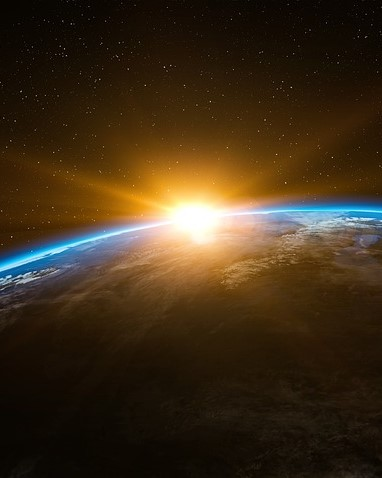
\includegraphics[width=\paperwidth,height=\paperheight]{space2}}; % original picture size was 8.08"x11.56"
\draw (current page.south) node [fill=white!30!white,fill opacity=0.6,text opacity=1,inner sep=1cm, anchor=south]{\Huge\centering\bfseries\sffamily\parbox[c][][t]{\paperwidth}{\centering \textsc{Systems Thinking, Engineering, and Analysis}\\[21pt] % Book title
{\huge Doctor Wolter J Fabrycky}}}; % Author name
\end{tikzpicture}
\vfill
\endgroup
%%----------------------------------------------------------------------------------------
%	COPYRIGHT PAGE
%%----------------------------------------------------------------------------------------
\newpage
~\vfill
\thispagestyle{empty}
\noindent Copyright \copyright\ 2018 Wolter J Fabrycky\\ % Copyright notice
\noindent \textsc{Published by ACE, a Zachary D Miller company}\\ % Publisher
\noindent \textsc{\url{www.a2i2.com}}\\ % URL
\noindent Licensed under the Creative Commons Attribution-NonCommercial 3.0 Unported License (the ``License''). You may not use this file except in compliance with the License. You may obtain a copy of the License at \url{http://creativecommons.org/licenses/by-nc/3.0}. Unless required by applicable law or agreed to in writing, software distributed under the License is distributed on an \textsc{``as is'' basis, without warranties or conditions of any kind}, either express or implied. See the License for the specific language governing permissions and limitations under the License.\\ % License information
\noindent \textit{First electronic publication, 2018} % Printing/edition date
%%----------------------------------------------------------------------------------------
%	TABLE OF CONTENTS
%%----------------------------------------------------------------------------------------
%\usechapterimagefalse % If you don't want to include a chapter image, use this to toggle images off - it can be enabled later with \usechapterimagetrue
\chapterimage{chain.jpg} % Table of contents heading image
\pagestyle{empty} % No headers
\tableofcontents % Print the table of contents itself
% undesirable as an e-book
%\cleardoublepage % Forces the first chapter to start on an odd page so it's on the right
\pagestyle{fancy} % Print headers again

% EXAMPLE TO WRITE EQUATIONS
\newpage
% no equations Chapter 1
% no equations Chapter 2
% no equations Chapter 3

\begin{equation} \label{stea-4-6-2-1}
\textrm{efficiency (physical)}=\frac{\textrm{output}}{\textrm{input}}
\end{equation}

\begin{equation} \label{stea-4-6-2-2}
\textrm{efficiency (economic)}=\frac{\textrm{worth}}{\textrm{cost}}
\end{equation}

\begin{equation} \label{stea-4-6-2-3}
\textrm{efficiency (economic)}=\frac{\textrm{Btu output}*\textrm{worth of electricity}}{\textrm{Btu input}*\textrm{cost of coal}}
\end{equation}
\newpage

% PROBLEMS / SOLUTIONS EXAMPLES
\newpage
%% SEA CHAPTER 1 - SYSTEMS SCIENCE AND ENGINEERING
\chapter{SYSTEMS SCIENCE AND ENGINEERING}

% SEA Question Location in \label{sea-Chapter#-Problem#}
\begin{exercises}
    \begin{exercise}
    \label{sea-1-26}
        Describe how systems thinking differs from systems engineering.
    \end{exercise}
    \begin{solution}
    \end{solution}
    
    \begin{exercise}
    \label{sea-1-1}
        For a system with which you are familiar, justify why it is a system according to the definition in \Cref{sec:sectorsComprisingWorld}.
    \end{exercise}
    \begin{solution}
    \end{solution}
    
    \begin{exercise} 
    \label{sea-1-2}
        Describe the components, attributes, and relationships in the system you used in Problem \ref{sea-1-1}.
    \end{exercise}
    \begin{solution}
    \end{solution}
    
    \begin{exercise}
    \label{sea-1-3}
        Name any system which includes a material that transforms over the system's life cycle and identify its structural components, operating components, and flow components.
    \end{exercise}
    \begin{solution}
    \end{solution}
    
    \begin{exercise} 
    \label{sea-1-4_5}
        Name any complex system and
        \begin{enumerate}[label=\alph*)]
            \item Define the hierarchy related to the system.
            \item Define the system boundaries.
        \end{enumerate}
    \end{exercise}
    \begin{solution}
    \end{solution}
    
    \begin{exercise} 
    \label{sea-1-6_7_8}
        Identify and contrast
        \begin{enumerate}[label=\alph*)]
            \item Physical versus conceptual systems.
            \item Static versus dynamic systems.
            \item Closed versus open systems.
        \end{enumerate}
    \end{exercise}
    \begin{solution}
    \end{solution}
    
    \begin{exercise} 
    \label{sea-1-15}
        For any system of the following types, name any system property
        \begin{enumerate}[label=\alph*)]
            \item Dynamic system.
            \item Steady-state system.
        \end{enumerate}
    \end{exercise}
    \begin{solution}
    \end{solution}
    
    \begin{exercise} 
    \label{sea-1-9}
        For each of the following systems, define a unique system and describe it in terms of components, attributes, and relationships
        \begin{enumerate}[label=\alph*)]
            \item Natural system.
            \item Human-made system.
            \item Human-modified system.
        \end{enumerate}
    \end{exercise}
    \begin{solution}
    \end{solution}
    
    \begin{exercise} 
    \label{sea-1-10_11_12}
        For the Human-made system in Question \ref{sea-1-9}
        \begin{enumerate}[label=\alph*)]
            \item Identify the system's purpose(s) and potential metrics to present its value.
            \item Describe the system's state at any arbitrary time during operation, at least one system behavior, and an overview of the system's process.
            \item Name any two related components of the system, define the purpose of each component as it relates to the other, and the necessary attributes of the component pair such that they contribute to the purpose(s) of the entire system.
        \end{enumerate}
    \end{exercise}
    \begin{solution}
    \end{solution}
    
    \begin{exercise} 
    \label{sea-1-14}
        For the Human-modified system in Question \ref{sea-1-9}, name some positive and negative impact(s) of the modification to the natural system.
    \end{exercise}
    \begin{solution}
    \end{solution}
    
    \begin{exercise} 
    \label{sea-1-13}
        Give examples of each of the following
        \begin{enumerate}[label=\alph*)]
            \item First-order relationship.
            \item Second-order relationship.
            \item Redundance.
        \end{enumerate}
    \end{exercise}
    \begin{solution}
    \end{solution}
    
    \begin{exercise} 
    \label{sea-1-16}
        Name any system that operates at equilibrium and another system that degrades over time.
    \end{exercise}
    \begin{solution}
    \end{solution}
    
    \begin{exercise} 
    \label{sea-1-17}
        The United States government, for example, can be divided and described as three individual entities of the executive, legislative, and judicial branches. Create an argument for why a government of this structure should either be considered a single system or three systems.
    \end{exercise}
    \begin{solution}
    \end{solution}
    
    \begin{exercise} 
    \label{sea-1-19}
        Give any example of cybernetics and define why the example is appropriate.
    \end{exercise}
    \begin{solution}
    \end{solution}
    
    \begin{exercise} 
    \label{sea-1-21}
        Do all systems at higher levels of Boulding's Hierarchy necessarily incorporate the lower levels of the hierarchy? If not, provide a specific system example.
    \end{exercise}
    \begin{solution}
    \end{solution}
    
    \begin{exercise} 
    \label{sea-1-22}
        Describe a novel system that may be necessary for society 50 to 100 years in the future and
        \begin{enumerate}[label=\alph*)]
            \item Define the system requirements.
            \item Define the system objectives.
        \end{enumerate}
    \end{exercise}
    \begin{solution}
    \end{solution}
    
    \begin{exercise} 
    \label{sea-1-25}
        For the system described in Question \ref{sea-1-22}
        \begin{enumerate}[label=\alph*)]
            \item Identify factors which led to the need for a new system.
            \item Identify other societal factors which may evolve in parallel and lead to other changes or innovations.
        \end{enumerate}
    \end{exercise}
    \begin{solution}
    \end{solution}
    
    \begin{exercise} 
    \label{sea-1-23}
        Compare and contrast systemology and synthesis.
    \end{exercise}
    \begin{solution}
    \end{solution}
    
    \begin{exercise} 
    \label{sea-1-24}
        Classify a technical system.
    \end{exercise}
    \begin{solution}
    \end{solution}
    
    \begin{exercise} 
    \label{sea-1-27}
        Compare and contrast the attributes of the Machine (Industrial) Age and the Systems Age.
    \end{exercise}
    \begin{solution}
    \end{solution}
    
    \begin{exercise} 
    \label{sea-1-28}
        Identify key differences between synthetic and analytical thinking. Is one method of thinking always preferable? Why or why not?
    \end{exercise}
    \begin{solution}
    \end{solution}
    
    \begin{exercise} 
    \label{sea-1-29}
        What challenges make the Systems Age unique from other periods of human evolution?
    \end{exercise}
    \begin{solution}
    \end{solution}
    
    \begin{exercise} 
    \label{sea-1-30}
        Compare and contrast systems engineering with other engineering disciplines.
    \end{exercise}
    \begin{solution}
    \end{solution}
    
    \begin{exercise} 
    \label{sea-1-32}
        Identify a system which required an interdisciplinary approach to develop \textit{or} to implement. What disciplines were required and why?
    \end{exercise}
    \begin{solution}
    \end{solution}
    
    \begin{exercise} 
    \label{sea-1-33}
        Identify an interdiscipline and the disciplines from which it was derived.
    \end{exercise}
    \begin{solution}
    \end{solution}
    
    \begin{exercise} 
    \label{sea-1-35_36_38}
        For the following organizations, summarize their mission statements
        \begin{enumerate}[label=\alph*)]
            \item \href{http://isss.org/world/index.php}{International Society for the Systems Sciences}
            \item \href{https://www.incose.org/}{International Council on Systems Engineering}
            \item \href{https://omegalpha.org/}{Omega Alpha Association}
        \end{enumerate}
    \end{exercise}
    \begin{solution}
    \end{solution}
    
    \begin{exercise} 
    \label{sea-1-37}
        Explain how the goals of ISSS and INCOSE differ.
    \end{exercise}
    \begin{solution}
    \end{solution}

\end{exercises}
% SKIPPED
% sea-1-18
% sea-1-20
% sea-1-31
% sea-1-34

%------------------------------------------------

%% SEA CHAPTER 2 - BRINGING SYSTEMS INTO BEING
\chapter{BRINGING SYSTEMS INTO BEING}

% SEA Question Location in \label{sea-Chapter#-Problem#}
\begin{exercises}
    \begin{exercise}
    \label{sea-2-1}
        Identify at least two characteristics that distinguish natural systems from those that are human-made or human-modified. 
    \end{exercise}
    \begin{solution}
    \end{solution}
    
    \begin{exercise}
    \label{sea-2-2}
        Identify at least two possible interfaces between the natural and human worlds for the creation of any arbitrary system.
    \end{exercise}
    \begin{solution}
    \end{solution}
    
    \begin{exercise}
    \label{sea-2-3}
        Describe what distinguishes human-made from human-modified systems.
    \end{exercise}
    \begin{solution}
    \end{solution}
    
    \begin{exercise}
    \label{sea-2-5_6}
        Based on the textbook descriptions in ???, identify a system for the following system types and justify your answer based on the system product(s).
        \begin{enumerate}[label=\alph*)]
            \item Single-entity product system.
            \item Multiple-entity product system.
        \end{enumerate}
    \end{exercise}
    \begin{solution}
    \end{solution}
    
    \begin{exercise}
    \label{sea-2-7_8}
        Choose any consumer item and identify the producer. Then
        \begin{enumerate}[label=\alph*)]
            \item Identify at least three things that are employed or consumed by the producer to create the consumer item.
            \item Identify any enabling system which is employed by the producer to create the consumer item.
            \item Must an enabling system and a product of that system be engineered jointly? Why or why not?
        \end{enumerate}
    \end{exercise}
    \begin{solution}
    \end{solution}
    
    \begin{exercise} 
    \label{sea-2-9}
        Identify at least four factors which determine a product's competitiveness. Is product competitiveness important? Why or why not?
    \end{exercise}
    \begin{solution}
        The quality, price, ergonomics, and lifetime of a product would all be considered to influence the purchasing behavior of consumers, which is based on product competition.
    \end{solution}
    
    \begin{exercise}
    \label{sea-2-10}
        Explain the benefits of system life-cycle thinking and why it is important. 
    \end{exercise}
    \begin{solution}
    \end{solution}
    
    \begin{exercise}
    \label{sea-2-11}
        For the product life-cycles displayed in figures ???, ???, identify possible sources of feedback or communication between the different phases.
    \end{exercise}
    \begin{solution}
    \end{solution}
    
    \begin{exercise}
    \label{sea-2-12}
        Pretend that you are developing a product. How do you convince your peer(s) that the best approach is to \say{design for the life cycle}?
    \end{exercise}
    \begin{solution}
    \end{solution}
    
    \begin{exercise}
    \label{sea-2-14} 
        Identify one benefit and one consequence of the following design models
        \begin{enumerate}[label=\alph*)]
            \item Waterfall model.
            \item Spiral model.
            \item V-model.
        \end{enumerate}
    \end{exercise}
    \begin{solution}
    \end{solution}
    
    \begin{exercise}
    \label{sea-2-14_part2}
        Of the models described in \ref{sea-2-14}, do you have a personal preference? Is any one model always the most appropriate? Why or why not? 
    \end{exercise}
    \begin{solution}
    \end{solution}
    
    \begin{exercise}
    \label{sea-2-15_16}
        Select a design situation of your choice.
        \begin{enumerate}[label=\alph*)]
            \item What are the requirements of the system?
            \item Describe the steps for identifying appropriate technical performance measures.
            \item Describe the relationship between the system requirements and its technical performance measures.
            \item What happens when the technical performance measures disagree with the system requirements?
        \end{enumerate}
    \end{exercise}
    \begin{solution}
    \end{solution}
    
    \begin{exercise}
    \label{sea-2-18_20}
        Select a design situation of your choice and refer to figure ??? for the following questions.
        \begin{enumerate}[label=\alph*)]
            \item Identify a top-level requirement and decompose it appropriately.
            \item Identify a lowest-level requirement and explain its relevance for all higher levels.
        \end{enumerate}
    \end{exercise}
    \begin{solution}
    \end{solution}
    
    \begin{exercise}
    \label{sea-2-22}
        Identify at least three domain manifestations of systems engineering.  
    \end{exercise}
    \begin{solution}
    \end{solution}
    
    \begin{exercise}
    \label{sea-2-23}
        Identify at least three obstructions which hinder or prevent the application of systems engineering.
    \end{exercise}
    \begin{solution}
    \end{solution}
    
    \begin{exercise}
    \label{sea-2-24}
        Why is systems thinking and engineering beneficial?
    \end{exercise}
    \begin{solution}
    \end{solution}

\end{exercises}
% SKIPPED
% sea-2-4
% sea-2-13
% sea-2-17
% sea-2-19
% sea-2-21
% sea-2-25
% sea-2-26

%------------------------------------------------

%% SEA CHAPTER 3 - CONCEPTUAL SYSTEM DESIGN
\chapter{CONCEPTUAL SYSTEM DESIGN}

% SEA Question Location in \label{sea-Chapter#-Problem#}
\begin{exercises}
    \begin{exercise}
    \label{sea-3-1}
    
    \end{exercise}
    \begin{solution}
    \end{solution}

\end{exercises}
% SKIPPED

%------------------------------------------------

%% SEA CHAPTER 4 - PRELIMINARY SYSTEM DESIGN
\chapter{PRELIMINARY SYSTEM DESIGN}

% SEA Question Location in \label{sea-Chapter#-Problem#}
\begin{exercises}
    \begin{exercise}
    \label{sea-4-1}
    
    \end{exercise}
    \begin{solution}
    \end{solution}

\end{exercises}
% SKIPPED

%------------------------------------------------

%% SEA CHAPTER 5 - DETAIL DESIGN AND DEVELOPMENT
\chapter{DETAIL DESIGN AND DEVELOPMENT}

% SEA Question Location in \label{sea-Chapter#-Problem#}
\begin{exercises}
    \begin{exercise}
    \label{sea-5-1}
    
    \end{exercise}
    \begin{solution}
    \end{solution}

\end{exercises}
% SKIPPED

%------------------------------------------------

%% SEA CHAPTER 6 - SYSTEM TEST, EVALUATION, AND VALIDATION
\chapter{SYSTEM TEST, EVALUATION, AND VALIDATION}

% SEA Question Location in \label{sea-Chapter#-Problem#}
\begin{exercises}
    \begin{exercise}
    \label{sea-6-1}
    
    \end{exercise}
    \begin{solution}
    \end{solution}

\end{exercises}
% SKIPPED

%------------------------------------------------

%% SEA CHAPTER 7 - ALTERNATIVES AND MODELS IN DECISION MAKING
\chapter{ALTERNATIVES AND MODELS IN DECISION MAKING}

% SEA Question Location in \label{sea-Chapter#-Problem#}
\begin{exercises}
    \begin{exercise}
    \label{sea-7-1}
    
    \end{exercise}
    \begin{solution}
    \end{solution}

\end{exercises}
% SKIPPED

%------------------------------------------------

%% SEA CHAPTER 8 - MODELS FOR ECONOMIC EVALUATION
\chapter{MODELS FOR ECONOMIC EVALUATION}

% SEA Question Location in \label{sea-Chapter#-Problem#}
\begin{exercises}
    \begin{exercise}
    \label{sea-8-1}
        How much money must be invested to accumulate \$10,000 in 8 years at 6\% compounded annually?
    \end{exercise}
    \begin{solution}
    \begin{equation}
        P=P/F,6,8=\$10,000
    \end{equation}
    \end{solution}
    
    \begin{exercise}
    \label{sea-8-2}
        What amount will be accumulated by each of the following investments?
        \begin{enumerate}[label=\alph*)]
            \item \$8,000 at 7.2\% compounded annually over 10 years.
            \item \$52,000 at 8\% compounded annually over 5 years.
        \end{enumerate}
    \end{exercise}
    \begin{solution}
    \end{solution}
    
    \begin{exercise}
    \label{sea-8-3}
        What is the present equivalent amount of a year-end series of receipts of \$6,000 over 5 years at 8\% compounded annually?
    \end{exercise}
    \begin{solution}
    \end{solution}
    
    \begin{exercise}
    \label{sea-8-4}
        What is the present equivalent of a year-end series of receipts starting with a first-year base of \$1,000 and increasing by 8\% per year to year 20 with an interest rate of 8\%?
    \end{exercise}
    \begin{solution}
    \end{solution}
    
    \begin{exercise}
    \label{sea-8-5}
        What is the present equivalent of a year-end series of receipts starting with a first-year base of \$1 million and decreasing by 25\% per year to year 4 with an interest rate of 6\%?
    \end{exercise}
    \begin{solution}
    \end{solution}
    
    \begin{exercise}
    \label{sea-8-6}
        What interest rate compounded annually is involved if \$4,000 results in \$10,000 in 6 years?
    \end{exercise}
    \begin{solution}
    \end{solution}
    
    \begin{exercise}
    \label{sea-8-7}
        How many years will it take for \$4,000 to grow to \$7,000 at an interest rate of 10\% compounded annually?
    \end{exercise}
    \begin{solution}
    \end{solution}
    
    \begin{exercise}
    \label{sea-8-8}
        What interest rate is necessary for a sum of money to double itself in 8 years? What is the approximate product of $i$ and $n$ ($i$ as an integer) that establishes the doubling period? How accurate is this product of $i$ and $n$ for estimating the doubling period?
    \end{exercise}
    \begin{solution}
    \end{solution}
    
    \begin{exercise}
    \label{sea-8-9}
        An asset was purchased for \$52,000 with the anticipation that it would serve for 12 years and be worth \$6000 as scrap. After 5 years of operation, the asset was sold for \$18,000. The interest rate is 14\%.
        \begin{enumerate}[label=\alph*)]
            \item What was the anticipated annual equivalent cost of the asset?
            \item What was the actual annual equivalent cost of the asset?
        \end{enumerate}
    \end{exercise}
    \begin{solution}
    \end{solution}
    
    \begin{exercise}
    \label{sea-8-10}
        An epoxy mixer purchased for \$33,000 has an estimated salvage value of \$5,000 and an expected life of 3 years. An average of 200 pounds per month will be processed by the mixer.
        \begin{enumerate}[label=\alph*)]
            \item Calculate the annual equivalent cost of the mixer with an interest rate of 8\%.
            \item Calculate the annual equivalent cost per pound mixed with an interest rate of 12\%.
        \end{enumerate}
    \end{exercise}
    \begin{solution}
    \end{solution}
    
    \begin{exercise}
    \label{sea-8-11}
        The table below shows the receipts and disbursements for a given venture. Determine the desirability of the venture for a 14\% interest rate, based on the present equivalent comparison and the annual equivalent comparison.
        \begin{table}[h]
        \centering
        \begin{tabular}{c r r}
        \toprule
        \textbf{End of the Year} & \textbf{Receipts (\$)} & \textbf{Disbursements (\$)}\\
        \midrule
        0 & 0 & 20,000 \\
        1 & 6,000 & 0 \\
        2 & 5,000 & 4,000 \\
        3 & 5,000 & 0 \\
        4 & 12,000 & 1,000 \\
        \bottomrule
        \end{tabular}
        %\caption{Table caption}
        \label{tab:example} % Unique label used for referencing the table in-text
        %\addcontentsline{toc}{table}{Table \ref{tab:example}} % Uncomment to add the table to the table of contents
        \end{table}
    \end{exercise}
    \begin{solution}
    \end{solution}
    
    \begin{exercise}
    \label{sea-8-12}
        A microcomputer-based controller can be installed for \$30,000 and will have a \$3,000 salvage value after 10 years and is expected to decrease energy consumption cost by \$4,000 per year.
        \begin{enumerate}[label=\alph*)]
            \item What rate of return is expected if the controller is used for 10 years?
            \item For what life will the controller give a return of 15\%?
        \end{enumerate}
    \end{exercise}
    \begin{solution}
    \end{solution}
    
    \begin{exercise}
    \label{sea-8-13}
        Transco plans on purchasing a bus for \$75,000 that will have a capacity of 40 passengers. As an alternative, a larger bus can be purchased for \$95,000 which will have a capacity of 50 passengers. The salvage value of either bus is estimated to be \$8,000 after a 10-year life. If an annual net profit of \$400 can be realized per passenger, which alternative should be recommended using a management-suggested interest rate of 15\%? Using the actual cost of money at 7.5\%?
    \end{exercise}
    \begin{solution}
    \end{solution}
    
    \begin{exercise}
    \label{sea-8-14}
        An office building and its equipment are insured to \$7,100,000. The present annual insurance premium is \$0.85 per \$100 of coverage. A sprinkler system with an estimated life of 20 years and no salvage value can be installed for \$180,000. Annual maintenance and operating cost is estimated to be \$3,600. The premium will be reduced to \$0.40 per \$100 coverage if the sprinkler system is installed.
        \begin{enumerate}[label=\alph*)]
            \item Find the rate of return if the sprinkler system is installed.
            \item With interest at 12\%, find the payout period for the sprinkler system.
        \end{enumerate}
    \end{exercise}
    \begin{solution}
    \end{solution}
    
    \begin{exercise}
    \label{sea-8-15}
        The design of a system is to be pursued from one of two available alternatives. Each alternative has a life-cycle cost associated with an expected future. The costs for the corresponding futures are given in the table below (in millions of dollars). If the probabilities of occurrence of the futures are 30\%, 50\%, and 20\%, respectively, which alternative is most desirable from an expected cost viewpoint, using an interest rate of 10\%?
        \begin{table}[h]
        \centering
        \begin{tabular}{l D{.}{.}{1} D{.}{.}{1} D{.}{.}{1} D{.}{.}{1} D{.}{.}{1} D{.}{.}{1} D{.}{.}{1} D{.}{.}{1} D{.}{.}{1} D{.}{.}{1} D{.}{.}{1} D{.}{.}{1}}
        \toprule
        \textbf{Design 1} & \multicolumn{12}{c}{\textbf{Years}} \\
        \midrule
        Future & 1 & 2 & 3 & 4 & 5 & 6 & 7 & 8 & 9 & 10 & 11 & 12 \\
        \midrule
        Optimistic & 0.4 & 0.6 & 5.0 & 7.0 & 0.8 & 0.8 & 0.8 & 0.8 & 0.8 & 0.8 & 0.8 & 0.8 \\
        Expected & 0.6 & 0.8 & 1.0 & 5.0 & 10.0 & 1.0 & 1.0 & 1.0 & 1.0 & 1.0 & 1.0 & 1.0 \\
        Pessimistic & 0.8 & 0.9 & 1.0 & 7.0 & 10.0 & 1.2 & 1.2 & 1.2 & 1.2 & 1.2 & 1.2 & 1.2 \\
        \midrule
        \textbf{Design 2} & \multicolumn{12}{c}{\textbf{Years}} \\
        \midrule
        Future & 1 & 2 & 3 & 4 & 5 & 6 & 7 & 8 & 9 & 10 & 11 & 12 \\
        \midrule
        Optimistic & 0.4 & 0.4 & 0.4 & 1.0 & 3.0 & 2.5 & 2.5 & 2.5 & 2.5 & 2.5 & 2.5 & 2.5 \\
        Expected & 0.6 & 0.8 & 1.0 & 3.0 & 6.0 & 3.0 & 3.0 & 3.0 & 3.0 & 3.0 & 3.0 & 3.0 \\
        Pessimistic & 0.6 & 0.8 & 1.0 & 5.0 & 6.0 & 3.1 & 3.1 & 3.1 & 3.1 & 3.1 & 3.1 & 3.1 \\
        \bottomrule
        \end{tabular}
        %\caption{Table caption}
        \label{tab:sea-8-15} % Unique label used for referencing the table in-text
        %\addcontentsline{toc}{table}{Table \ref{tab:example}} % Uncomment to add the table to the table of contents
        \end{table}
    \end{exercise}
    \begin{solution}
    \end{solution}
    
    \begin{exercise}
    \label{sea-8-16}
        Prepare a decision evaluation matrix for the design alternatives in \ref{sea-8-15}, and then choose the alternative that is best under the following decision rules: Laplace, maximax, maximin, and Hurwicz with $\alpha=0.6$. Assume that the choice is under uncertainty.
    \end{exercise}
    \begin{solution}
    \end{solution}
    
    \begin{exercise}
    \label{sea-8-17}
        A campus laboratory can be climate conditioned by piping chilled water from a central refrigeration plant. Two competing proposals are being considered for the piping system, as outlined in the table. On the basis of a 10-year life, find the number of hours of operation per year for which the cost of the two systems will be equal if the interest rate is 9\%.
        \begin{table}[h]
        \centering
        \begin{tabular}{l D{.}{.}{2} D{.}{.}{2}}
        \toprule
        {} & \textbf{6" System} & \textbf{8" System}\\
        \cmidrule{2-3}
        {} & \multicolumn{2}{c}{Horsepower} \\
        \cmidrule{2-3}
        Motor size & 6 & 3 \\
        \midrule
        {} & \multicolumn{2}{c}{Cost (\$)} \\
        \cmidrule{2-3}
        Pump and pipe installation & 32,000 & 44,000 \\
        Motor installation & 4,500 & 3,000 \\
        Energy per hour of operation & 3.20 & 2.00 \\
        \midrule
        Salvage value & 5,000 & 6,000 \\
        \bottomrule
        \end{tabular}
        %\caption{Table caption}
        \label{tab:sea-8-17} % Unique label used for referencing the table in-text
        %\addcontentsline{toc}{table}{Table \ref{tab:example}} % Uncomment to add the table to the table of contents
        \end{table}
    \end{exercise}
    \begin{solution}
    \end{solution}
    
    \begin{exercise}
    \label{sea-8-18}
        Replacement fence posts for a cattle ranch are currently purchased for \$4.20 each. It is estimated that equivalent posts can be cut from timber on the ranch for a variable cost of \$1.50 each, which is made up of the value of the timber plus labor cost. Annual fixed cost for required equipment is estimated to be \$1,200. If 1,000 posts will be required each year, What will be the annual saving if posts are cut?
    \end{exercise}
    \begin{solution}
    \end{solution}
    
    \begin{exercise}
    \label{sea-8-19}
        An equipment operator can buy a maintenance component from a supplier for \$960 per unit delivered. Alternatively, operator can rebuild the component for a variable cost of \$460 per unit. It is estimated that the additional fixed cost would be \$80,000 per year if the component is rebuilt. Find the number of units per year for which the cost of the two alternatives will break even.
    \end{exercise}
    \begin{solution}
    \end{solution}
    
    \begin{exercise}
    \label{sea-8-20}
        A marketing company can lease a fleet of automobiles for its sales personnel for \$35 per day plus \$0.18 per mile for each vehicle. As an alternative, the company can pay each salesperson \$0.45 per mile to use his or her own automobile. If these are the only costs to the company, how many miles per day must a salesperson drive for the two alternatives to break even?
    \end{exercise}
    \begin{solution}
    \end{solution}
    
    \begin{exercise}
    \label{sea-8-21}
        An electronics manufacturer is considering the purchase of one of two types of laser trimming devices. The sales forecast indicated that at least 8,000 units will be sold per year. Device A will increase the annual fixed cost of the plant by \$20,000 and will reduce variable cost by \$5.60 per unit. Device B will increase the annual fixed cost by \$5,000 and will reduce variable cost by \$3.60 per unit. If variable costs are now \$20 per unit produced, which device should be purchased?
    \end{exercise}
    \begin{solution}
    \end{solution}
    
    \begin{exercise}
    \label{sea-8-22}
        Machine A costs \$20,000, has zero salvage value at any time, and has an associated labor cost of \$1.15 for each piece produced on it. Machine B costs \$36,000, has zero salvage value at any time, and has an associated labor cost of \$0.90. Neither machine can be used except to produce the product described. If the interest rate is 10\% and the annual rate of production is 20,000 units, how many years will it take for the cost of the two machines to break even?
    \end{exercise}
    \begin{solution}
    \end{solution}
    
    \begin{exercise}
    \label{sea-8-23}
        An electronics manufacturer is considering two methods for producing a circuit board. The board can be hand-wired at an estimated cost of \$9.80 per unit and an annual fixed equipment cost of \$10,000. A printed equivalent can be produced using equipment costing \$180,000 with a service life of 8 years and salvage value of \$12,000. It is estimated that the labor cost will be \$3.20 per unit and that the processing equipment will cost \$4,000 per year to maintain. If the interest rate is 8\%, how many circuit boards must be produced each year for the two methods to break even?
    \end{exercise}
    \begin{solution}
    \end{solution}
    
    \begin{exercise}
    \label{sea-8-24}
        It is estimated that the annual sales of labor-saving device will be 20,000 the first year and increase by 10,000 per year until 50,000 units are sold during the fourth year. Proposal A is to purchase manufacturing equipment costing \$120,000 with an estimated salvage value of \$15,000 at the end of 4 years. Proposal B is to purchase equipment costing \$280,000 with an estimated salvage value of \$32,000 at the end of 4 years. The variable manufacturing cost per unit under proposal A is estimated to be \$8.00, but is estimated to be only \$0.26 under proposal B. If the interest rate is 9\%, which proposal should be accepted for a 4-year production period?
    \end{exercise}
    \begin{solution}
    \end{solution}
    
    \begin{exercise}
    \label{sea-8-25}
        The fixed operating cost of a machine center (capital recovery, interest, maintenance, space charges, supervision, insurance, and taxes) is $F$ dollars per year. The variable cost of operating the center (power, supplies, and other items, but excluding direct labor) is $V$ dollars per hour of operation. If $N$ is the number of hours the center is operated per year, $TC$ the annual total cost of operating the center, $TC_h$ the hourly cost of operating the center, $t$ the time in hours to process 1 unit of product, and $M$ the center cost of processing 1 unit, write expressions for the following
        \begin{enumerate}[label=\alph*)]
            \item $TC$
            \item $TC_h$
            \item $M$
        \end{enumerate}
    \end{exercise}
    \begin{solution}
    \end{solution}
    
    \begin{exercise}
    \label{sea-8-26}
        In \ref{sea-8-25}, $F=\$60,000$ per year, $t=0.2$ hour, $V=\$50$ per hour, and $N$ varies from 1,000 to 10,000 in increments of 1,000.
        \begin{enumerate}[label=\alph*)]
            \item Plot values of $M$ as a function of $N$.
            \item Write an expression for the total cost of direct labor and machine cost per unit $TC_h$ using the symbols in \ref{sea-8-25} and letting $W$ equal the hourly cost of direct labor.
        \end{enumerate}
    \end{exercise}
    \begin{solution}
    \end{solution}
    
    \begin{exercise}
    \label{sea-8-27}
        A certain firm has the capacity to produce 800,000 units per year. At present it is operating at 75\% of capacity. The income per unit is \$0.10 regardless of output. Annual fixed costs are \$28,000, and the variable cost is \$0.06 per unit. Find the annual profit or loss at this capacity and the capacity for which the firm will break even.
    \end{exercise}
    \begin{solution}
    \end{solution}
    
    \begin{exercise}
    \label{sea-8-28}
        An arc welding machine that is used for a certain joining process costs \$90,000. The machine has a life of 5 years and a salvage value of \$10,000. Maintenance, taxes, insurance, and other fixed costs amount to \$5,000 per year. The cost of power and supplies is \$28.00 per hour of operation and the total operator cost (direct and indirect) is \$65.00 per hour. If the cycle time per unit of product is 60 min and the interest rate is 8\%, calculate the cost per unit for the following unit outputs per year.
        \begin{enumerate}[label=\alph*)]
            \item 200 units
            \item 600 units
            \item 1,800 units
        \end{enumerate}
    \end{exercise}
    \begin{solution}
    \end{solution}
    
    \begin{exercise}
    \label{sea-8-29}
        A certain processing center has the capacity to assemble 650,000 units per year. At present, it is operating at 65\% of capacity. The annual income is \$416,000. Annual fixed costs are \$192,000 and the variable costs are \$0.38 per unit assembled.
        \begin{enumerate}[label=\alph*)]
            \item What is the annual profit or loss attributable to the center?
            \item At what volume of output does the center break even?
            \item What will be the profit or loss at 70\%, 80\%, and 90\% of capacity on the basis of constant income per unit and constant variable cost per unit?
        \end{enumerate}
    \end{exercise}
    \begin{solution}
    \end{solution}
    
    \begin{exercise}
    \label{sea-8-30}
        Chemco operates two plants, A and B, which produce the same product. The capacity of plant A is 60,000 gallons while that of B is 80,000 gallons. The annual fixed cost of plant A is \$2,600,000 per year and the variable cost is \$32 per gallon. The corresponding values for plant B are \$2,800,000 and \$39 per gallon. At present, plant A is being operated at 35\% of capacity and plant B is being operated at 40\% of capacity.
        \begin{enumerate}[label=\alph*)]
            \item What would be the total cost of production of plants A and B?
            \item What are the total cost and the average unit cost of the total output of both plants?
            \item What would be the total cost to the company and cost per gallon if all production were transferred to plant A?
            \item What would be the total cost to the company and cost per gallon if all production were transferred to plant B?
        \end{enumerate}
    \end{exercise}
    \begin{solution}
    \end{solution}

\end{exercises}
% SKIPPED

%------------------------------------------------

%% SEA CHAPTER 9 - OPTIMIZATION IN DESIGN AND OPERATIONS
\chapter{OPTIMIZATION IN DESIGN AND OPERATIONS}

% SEA Question Location in \label{sea-Chapter#-Problem#}
\begin{exercises}
    \begin{exercise}
    \label{sea-9-1}
        Specify the dimensions of the sides of a rectangle of perimeter $p$ so that the area it encloses will be maximum.
    \end{exercise}
    \begin{solution}
    \end{solution}
    
    \begin{exercise}
    \label{sea-9-2}
        The cost per unit produced at a certain facility is represented by the function
        \begin{equation}
            UC = 2x^2-10x+50
        \end{equation}
        where $x$ is in thousands of units produced. For what value of $x$ would unit cost be minimized (other than zero)? What is the minimum cost at this volume? Show that the value found is truly a minimum.
    \end{exercise}
    \begin{solution}
    \end{solution}
    
    \begin{exercise}
    \label{sea-9-3}
        Advertising expenditures have been found to relate to profit approximately in accordance with the function
        \begin{equation}
            P = x^3-100x^2+3,125x
        \end{equation}
        where $x$ is the expenditure in thousands of dollars. What advertising expenditure would produce the maximum profit? What profit is expected at this expenditure? Show that the derived result is truly a maximum.
    \end{exercise}
    \begin{solution}
    \end{solution}
    
    \begin{exercise}
    \label{sea-9-4}
        The cost of producing and selling a certain item is for the first 1,000 units, for a production range between 1,000 and 2,500 units, and $\$205x-\$97.500$ for more than 2,500 units, where $x$ is the number of units produced. If the selling price is \$200 per unit, and all units produced are sold,find the level of production that will maximize profit.
    \end{exercise}
    \begin{solution}
    \end{solution}
    
    \begin{exercise}
    \label{sea-9-5}
        Ethyl acetate is made from acetic acid and ethyl alcohol. Let $x=$ pounds of acetic acid input, $y=$ of ethyl alcohol input, and $z=$ of ethyl acetate output. The relationship of output to input is
        \begin{equation}
            \frac{z^2}{(1.47x-z)(1.91y-z)}=3.9
        \end{equation}
        \begin{enumerate}[label=\alph*)]
            \item Determine the output of ethyl acetate per pound of acetic acid,where the ratio of acetic acid of ethyl alcohol is 2.0,1.0,and 0.67,and graph the result.
            \item Graph the cost of material per pound of ethyl acetate for each of the ratios given and determine the ratio for which the material cost per pound of ethyl acetate is a minimum if acetic acid costs \$0.80 per pound and ethyl alcohol costs \$0.92 per pound.
        \end{enumerate}
    \end{exercise}
    \begin{solution}
    \end{solution}
    
    \begin{exercise}
    \label{sea-9-6}
        It has been found that the heat loss through the ceiling of a building is 0.13 Btu per hour per square foot of area per degree Fahrenheit. If the $2,200ft^2$ ceiling is insulated,the heat loss in Btu per hour per degree temperature difference per square foot of area is taken as
        \begin{equation}
            \frac{1}{(\frac{1}{0.13})(\frac{t}{0.27})}
        \end{equation}
        where tis the thickness in inches.The in-place cost of insulation 2,4,and 6 in thick is \$0.18, \$0.30,and \$0.44 per square foot,respectively.The building is heated to 75$^{\circ}$F 3,000 hrs per year by a gas furnace with an efficiency of 50\%.The mean outside temperature is 45°F and the natural gas used in the furnace costs \$4.40 per and has a heating value of 2,000 Btu per What thickness of insulation, if any, should be used if the interest rate is 10\% and the resale value of the building 6 years hence is enhanced \$850 if insulation is added,regardless of the thickness?
    \end{exercise}
    \begin{solution}
    \end{solution}
    
    \begin{exercise}
    \label{sea-9-7}
        An overpass is being considered for a certain crossing. The superstructure design under consideration will be made of reinforced concrete and will have a weight per foot depending on the span between piers in accordance with $W=32(S)+1,850$. Piers will be made of steel and will cost \$250,000 each. The superstructure will be erected at a cost of \$3.20 per pound. If the number of piers required is to be one less than the number of spans, find the number of piers that will result in a minimum total cost for piers and superstructure if $L=1,250$ft. 
    \end{exercise}
    \begin{solution}
    \end{solution}
    
    \begin{exercise}
    \label{sea-9-8}
        Two girder designs are under consideration for a bridge for a 1,200-foot crossing.The first is expected to result in a superstructure weight per foot of $22(S)+800$, where $S$ is the span between piers. The second should result in superstructure weight per foot of $20(S)+1,000$. Piers and two required abutments are estimated to cost \$220,000 each. The superstructure will be erected at a cost of \$0.55 per pound. Choose the girder design that will result in a minimum cost and specify the optimum number of piers.
    \end{exercise}
    \begin{solution}
    \end{solution}
    
    \begin{exercise}
    \label{sea-9-9}
        What is the cost advantage of choosing the best girder design for the bridge described in \ref{sea-9-8}? If the number of piers is determined from the best girder design alternative, but the other design alternative is adopted, what cost penalty is incurred?
    \end{exercise}
    \begin{solution}
    \end{solution}
    
    \begin{exercise}
    \label{sea-9-10}
        A used automobile can be purchased by a student to provide transportation to and from school for \$5,500 as is (i.e.,the auto will have no warranty). First-year maintenance cost is expected to be \$350 and the maintenance costs will increase by \$100 per year thereafter. Operation costs for the automobile will be \$1,200 for every year the auto is used and its salvage value decreases by 15\% per year.
        \begin{enumerate}[label=\alph*)]
            \item What is the economic life without considering the time value of money?
            \item With interest at 16\%,what is the economic life?
        \end{enumerate}
    \end{exercise}
    \begin{solution}
    \end{solution}
    
    

\end{exercises}
% SKIPPED

%------------------------------------------------

%% SEA CHAPTER 10 - QUEUING THEORY AND ANALYSIS

% SEA Question Location in \label{sea-Chapter#-Problem#}
\begin{exercises}
    \begin{exercise}
    \label{sea-10-1}
    
    \end{exercise}
    \begin{solution}
    \end{solution}

\end{exercises}
% SKIPPED

%------------------------------------------------

%% SEA CHAPTER 11 - CONTROL CONCEPTS AND METHODS

% SEA Question Location in \label{sea-Chapter#-Problem#}
\begin{exercises}
    \begin{exercise}
    \label{sea-11-1}
    
    \end{exercise}
    \begin{solution}
    \end{solution}

\end{exercises}
% SKIPPED

%------------------------------------------------

%% SEA CHAPTER 12 - DESIGN FOR OPERATIONAL FEASIBILITY

% SEA Question Location in \label{sea-Chapter#-Problem#}
\begin{exercises}
    \begin{exercise}
    \label{sea-12-1}
    
    \end{exercise}
    \begin{solution}
    \end{solution}

\end{exercises}
% SKIPPED

%------------------------------------------------

%% SEA CHAPTER 13 - DESIGN FOR MAINTAINABILITY

% SEA Question Location in \label{sea-Chapter#-Problem#}
\begin{exercises}
    \begin{exercise}
    \label{sea-13-1}
    
    \end{exercise}
    \begin{solution}
    \end{solution}

\end{exercises}
% SKIPPED

%------------------------------------------------

%% SEA CHAPTER 14 - DESIGN FOR USABILITY (HUMAN FACTORS)

% SEA Question Location in \label{sea-Chapter#-Problem#}
\begin{exercises}
    \begin{exercise}
    \label{sea-14-1}
    
    \end{exercise}
    \begin{solution}
    \end{solution}

\end{exercises}
% SKIPPED

%------------------------------------------------

%% SEA CHAPTER 15 - DESIGN FOR LOGISTICS AND SUPPORTABILITY

% SEA Question Location in \label{sea-Chapter#-Problem#}
\begin{exercises}
    \begin{exercise}
    \label{sea-15-1}
    
    \end{exercise}
    \begin{solution}
    \end{solution}

\end{exercises}
% SKIPPED

%------------------------------------------------

%% SEA CHAPTER 16 - DESIGN FOR PRODUCIBILITY, DISPOSABILITY, AND SUSTAINABILITY

% SEA Question Location in \label{sea-Chapter#-Problem#}
\begin{exercises}
    \begin{exercise}
    \label{sea-16-1}
    
    \end{exercise}
    \begin{solution}
    \end{solution}

\end{exercises}
% SKIPPED

%------------------------------------------------

%% SEA CHAPTER 17 - DESIGN FOR AFFORDABILITY (LIFE-CYCLE COSTING)

% SEA Question Location in \label{sea-Chapter#-Problem#}
\begin{exercises}
    \begin{exercise}
    \label{sea-17-1}
    
    \end{exercise}
    \begin{solution}
    \end{solution}

\end{exercises}
% SKIPPED

%------------------------------------------------

%% SEA CHAPTER 18 - SYSTEMS ENGINEERING PLANNING AND ORGANIZATION

% SEA Question Location in \label{sea-Chapter#-Problem#}
\begin{exercises}
    \begin{exercise}
    \label{sea-18-1}
    
    \end{exercise}
    \begin{solution}
    \end{solution}

\end{exercises}
% SKIPPED

%------------------------------------------------

%% SEA CHAPTER 19 - PROGRAM MANAGEMENT, CONTROL, AND EVALUATION

% SEA Question Location in \label{sea-Chapter#-Problem#}
\begin{exercises}
    \begin{exercise}
    \label{sea-19-1}
    
    \end{exercise}
    \begin{solution}
    \end{solution}

\end{exercises}
% SKIPPED

%------------------------------------------------
\newpage

%%%---------------------------------------------------------------------------------------
%%
%	PART I
%%
%%%---------------------------------------------------------------------------------------
%\part{SYSTEMS AND SYSTEMS THINKING}\label{part:1}

Systems engineering and analysis is promulgated most effectively when supported by insight about important system domains having high-level association.  That is the purpose of four chapters comprising \Cref{part:1} of this textbook.  The relevant domains are the world in which we live, systems thinking and knowledge, organization and enterprise systems, and economics and enterprise economy. Together these provide a prerequisite foundation for the synthesis, analysis, and evaluation of engineered systems; engineered systems being the central focus of this book.
	
The first chapter introduces the world in which we live as the overarching system of primary interest. When partitioned into interconnected natural, human-made, and human-modified sectors, it is found that human activities may be traced and evaluated at high levels with purpose and confidence.
	
\Cref{chap:2} has a science and systems science orientation.  It covers general system definitions and ends with contemporary definitions of systems engineering.  Between these important definitional categories is a conceptual discussion of system elements, a high-level classification of systems, a summary of science and systems science, and a view of technology as the progenitor for engineered systems.
	
Cooperation through organization is essential for human progress. It addressed in \Cref{chap:3} as humankind’s most important innovation. The role of purposeful human action, known as praxeology, is emphasized as being most relevant to systems thinking and enterprise systems.
	
Praxeology also underpins \Cref{chap:4}, focused on economics and enterprise economy.  Here the human action form of economic thinking is featured as the basis for economic progress. Taken together, these last two chapters address organization as humankind’s most important innovation within the pervasive economic setting for enterprises and the economy.

\Cref{part:1} of this textbook has the potential to stand alone as a learning module.  It provides a high-level introduction to systems, science, engineering, and systems engineering that will be suitable for discussion with engineering and technical people.  Subsequent chapters should be considered only after obtaining an understanding of the fundamentals in Part I, but study beyond these fundamentals is optional for those who need only an overview of systems engineering and its foundation in systems analysis.

%%----------------------------------------------------------------------------------------
%	  CHAPTER 1
%%----------------------------------------------------------------------------------------
%\chapterimage{purpleLeaf.jpg} % Chapter heading image
\chapter{THE WORLD IN WHICH WE LIVE} \label{chap:1}

The world in which we live is known more to us than is the universe or, perhaps, universes in which it exists.  This world is known to be part of a solar system which is known to be part of a universe made up of similar solar systems and galaxies.  We know more about the world in which we live than we do about the universe in which it resides.  In fact, the purposes of this textbook are realized independent of knowing any more of a universal nature extant above and beyond our world.

The primary purpose of this textbook may be addressed directly by recognizing the ultimate system of interest in STEA to be \textit{the world in which we live}.  We observe the \textit{natural}, the \textit{human-made}, and the \textit{human-modified} worlds to be interconnected sectors as illustrated in \Cref{fig:humanModifiedVennDiagram}.  Of these, it is the human-modified world that should be adopted as the highest-level system of our concern, because that is where we actually live.

\begin{figure}[h]
\centering
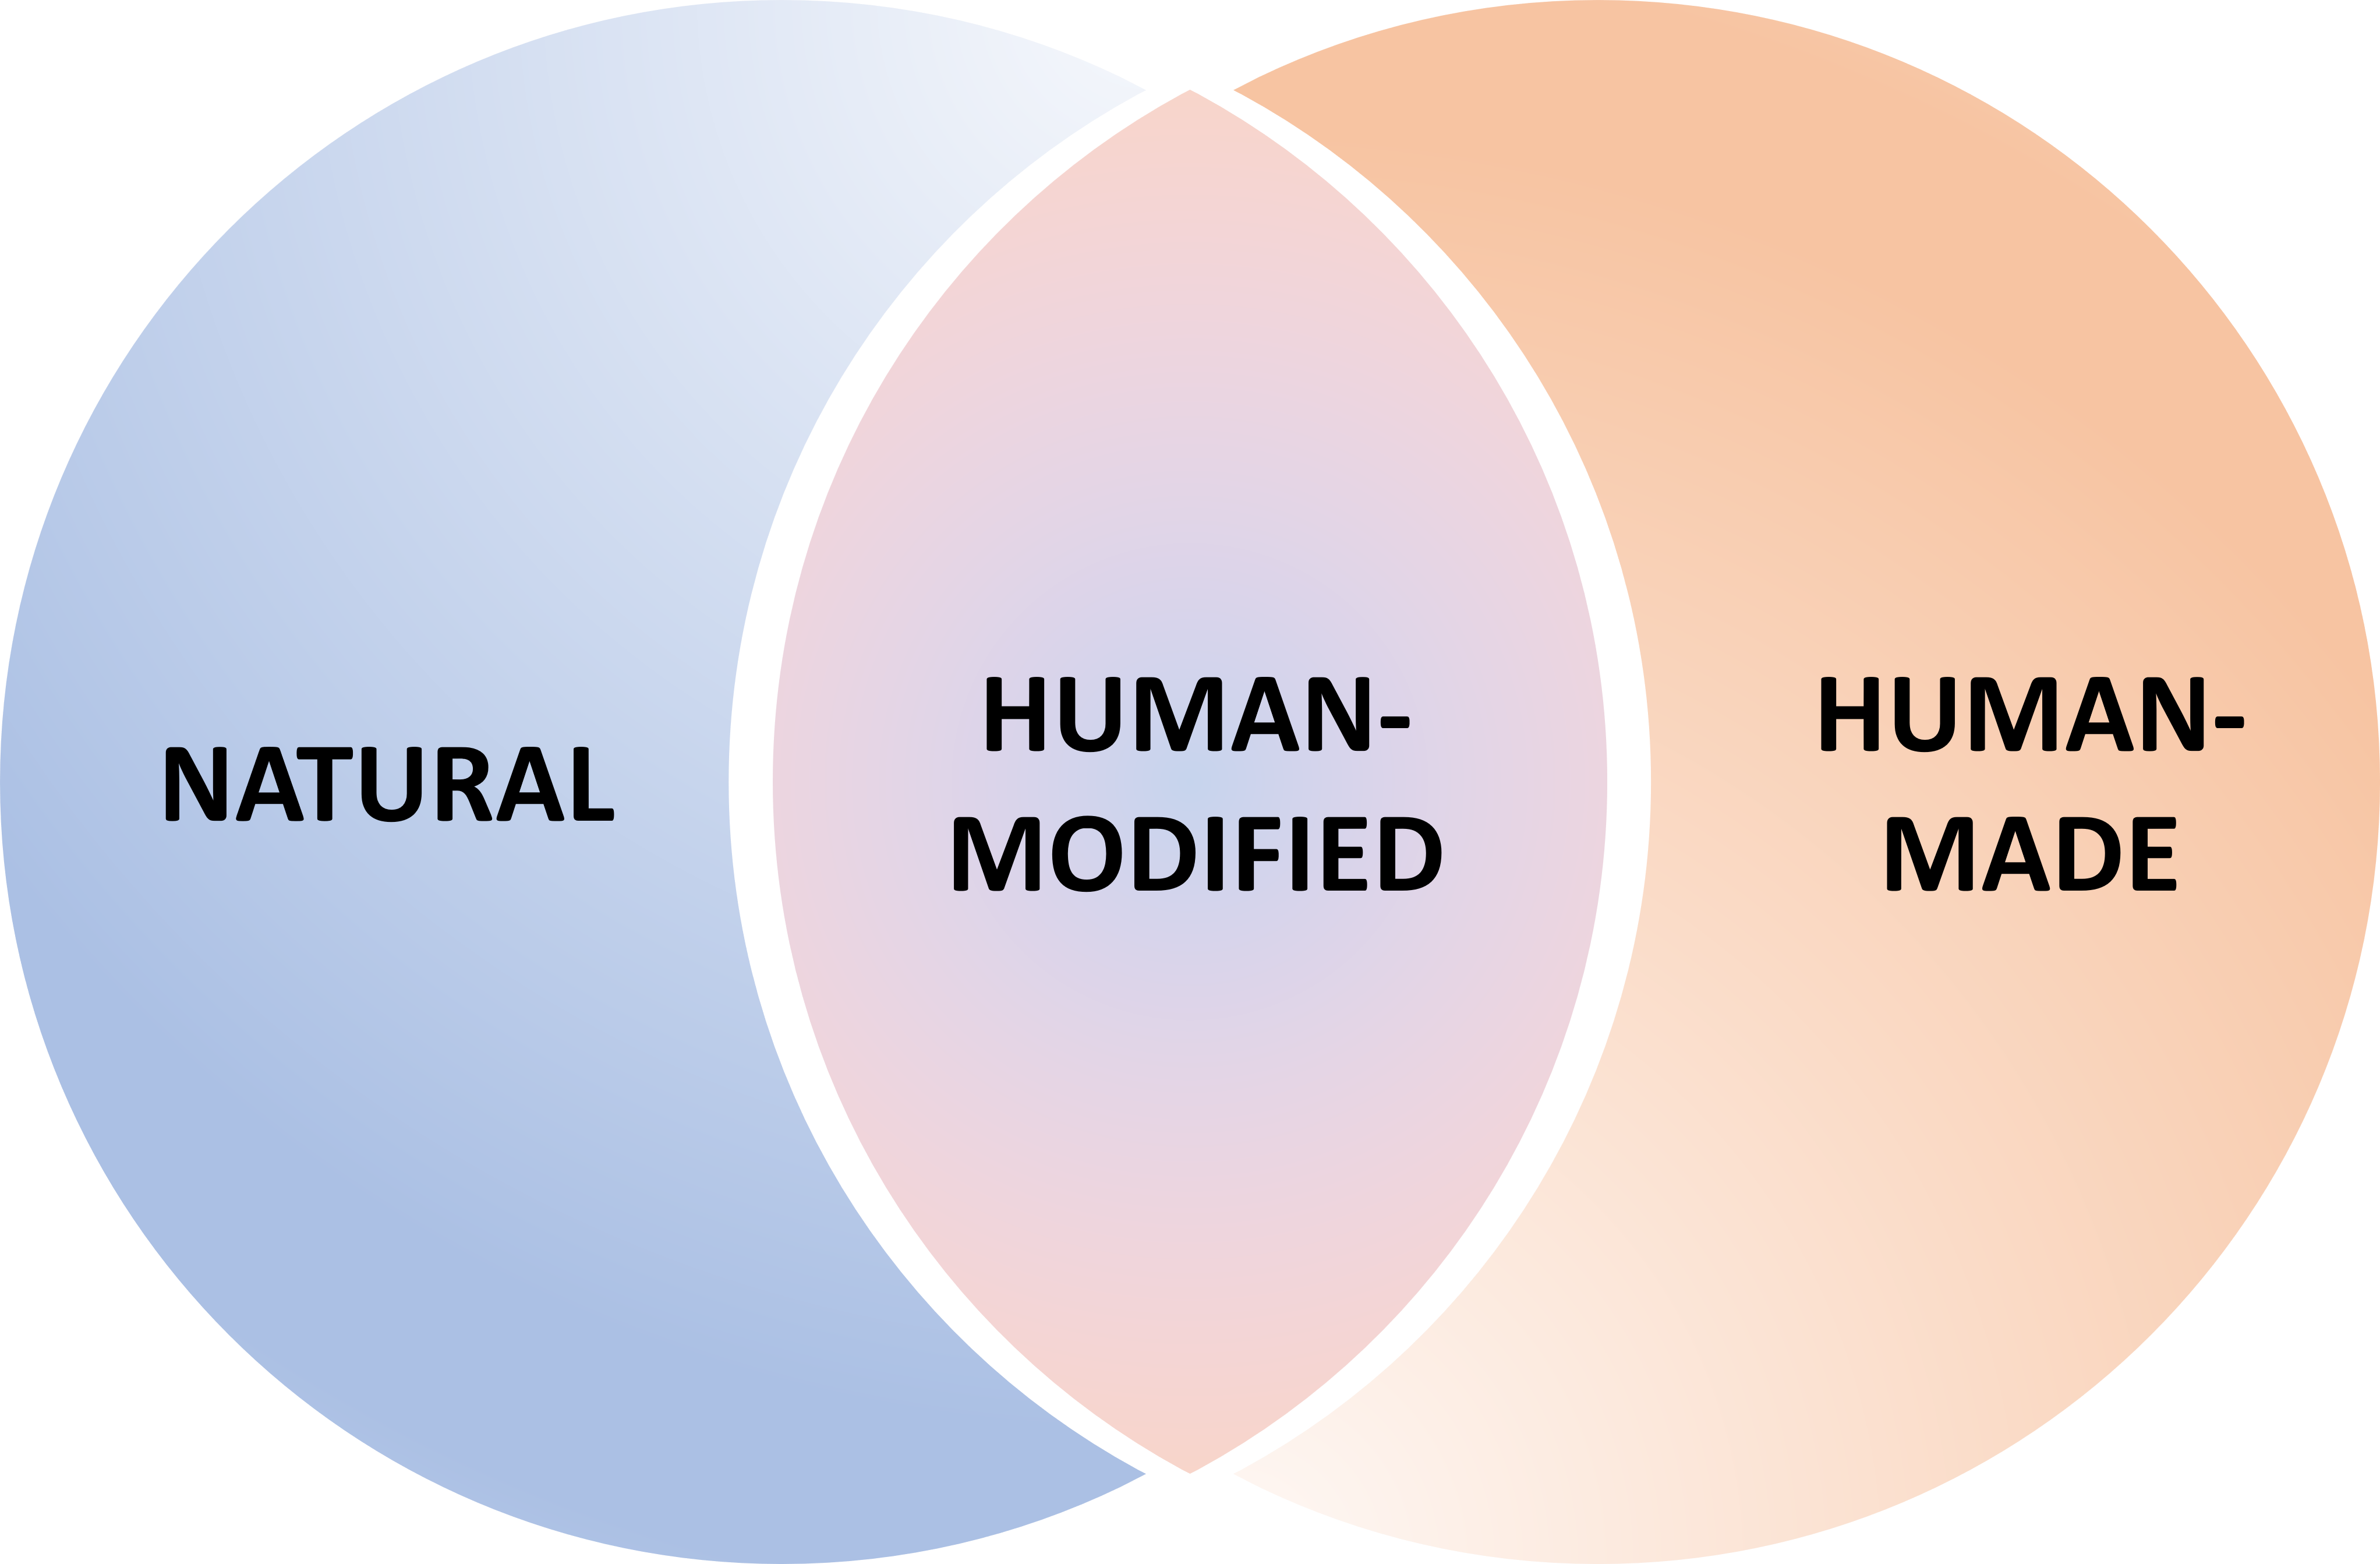
\includegraphics[width=0.9\textwidth]{humanModifiedVennDiagram.png}
\caption{Our world viewed as interconnected sectors.}
\label{fig:humanModifiedVennDiagram}
\end{figure}
    
The natural world came into being by natural processes.  The human-made world is made up of systems and products that resulted from the intervention of humans through components, attributes, and relationships.  The \textit{human-modified world} is the natural world into which the human-made has been introduced as systems, subsystems, entities, and artifacts; a world becoming increasingly complex.  This book strives to justify the human-modified world as the ultimate system level at which the viability of all that is human made should be judged.

\section{Sectors Comprising Our World}\index{Sectors Comprising Our World}\label{sec:sectorsComprisingWorld}

The world in which we live may be divided into the natural world and the human-made world.  Included in the former are all elements of the world that came into being by natural processes. The human-made world is made up of all human-originated systems, their product subsystems (including structures and services), and their other subsystems (such as those for production and support).  But it is the advent of the human-made that has resulted in a human-modified world as the actual world in which we live.

Systems are as pervasive as the universe in which they exist.  They are as grand as the universe itself or as infinitesimal as the atom.  This is, however, beyond the scope of STEA and requires reduction into sectors comprising our world.  Systems appeared first in natural forms, but with the advent of human beings a variety of human-made systems have come into existence.

The origin of systems gives the most important classification opportunity.  \textit{Natural systems} are those that came into being by natural processes.  \textit{Human-made systems} are those in which human beings have intervened through component, attributes, and relationships.  The \textit{human-modified system} is a natural system into which a human-made system has been integrated.

\subsection{The Natural World}\index{The Natural World}\label{sec:NaturalWorld}

The natural world is made up of all systems, including humans, that came into being by natural processes without human involvement. \textit{Natural systems} are those that came into being by natural processes. \textit{Human-made systems} are those in which human beings have intervened through components, attributes, and relationships. 

All human-made systems, when brought into being, are embedded into the natural world. Important interfaces often exist between human-made systems and natural systems. Each affects the other in some way. The effect of human-made systems on the natural world has only recently become a keen subject for study by concerned people, especially in those instances where the effect is undesirable. In some cases, this study is facilitated by analyzing the natural system as a human-modified system.

When designing a human-made system, undesirable effects can be minimized—and the natural system can sometimes be improved—by engineering the larger human-modified system instead of engineering only the human-made system. If analysis, evaluation, and validation of the human-modified system are appropriate, then the boundary of the environmental system—drawn to include the human-made system—should be considered the boundary of the human-modified system.

Natural systems exhibit a high degree of order and equilibrium. This is evidenced in the seasons, the food chain, the water cycle, and so on. Organisms and plant life adapt themselves to maintain equilibrium with the environment. Every event in nature is accompanied by an appropriate adaptation, one of the most important being that material flows are cyclic. In the natural environment there are no dead ends, no wastes, only continual re-circulation and regeneration.

Only recently have significant human-made systems appeared. These systems make up the human-made world, their chief engineer being human. The rapid evolution of human beings is not adequately understood, but their arrival has significantly affected the natural world, often in undesirable ways. Primitive beings had little impact on the natural world, for they had not yet developed potent and pervasive technologies.

An example of the impact of human-made systems on natural systems is the set of problems that arose from building the Aswan Dam on the Nile River. Construction of this massive dam ensures that the Nile will never flood again, solving an age-old problem. However, several new problems arose. The food chain was broken in the eastern Mediterranean, thereby reducing the fishing industry. Rapid erosion of the Nile Delta took place, introducing soil salinity into Upper Egypt. No longer limited by periodic dryness, the population of bilharzia (a waterborne snail parasite) has produced an epidemic of disease along the Nile. These side effects were not adequately anticipated by those responsible for the project. A system view encompassing both natural and human-made elements, as a human-modified system, might have led to a better solution to the problem of flooding. (Look for a better / more general example).


An example of the impact of human-made systems on natural systems is the set of problems that arose from building the Aswan Dam on the Nile River\footnote{\href{http://www.edc.uri.edu/temp/ci/ciip/FallClass/Docs_2006/UrbanWaterfronts/Abu-Zeid\%20and\%20El-Shibini.pdf}{Aswan Dam on the Nile}}. Construction of this massive dam ensures that the Nile will never flood again, solving an age-old problem. However, several new problems arose. The food chain was broken in the eastern Mediterranean, thereby reducing the fishing industry. Rapid erosion of the Nile Delta took place, introducing soil salinity into Upper Egypt. No longer limited by periodic dryness, the population of bilharzia (a waterborne snail parasite) has produced an epidemic of disease along the Nile. These side effects were not adequately anticipated by those responsible for the project. A system view encompassing both natural and human-made elements, as a human-modified system, might have led to a better solution to the problem of flooding.

\subsection{The Human-Made World}\index{The Human-Made World}\label{subsec:humanMadeWorld}

The human-made world is made up of all systems wherein humans have intervened through components, attributes, and relationships.

All human-made systems, when brought into being, are embedded into the natural world. Important interfaces often exist between human-made systems and natural systems. Each affects the other in some way. The effect of human-made systems on the natural world has only recently become a keen subject for study by concerned people, especially in those instances where the effect is undesirable. In some cases, this study is facilitated by analyzing the natural system as a human-modified system.

When designing a human-made system, undesirable effects can be minimized - and the natural system can sometimes be improved - by engineering the larger human-modified system instead of engineering only the human-made system. If analysis, evaluation, and validation of the human-modified system are appropriate, then the boundary of the environmental system - drawn to include the human-made system - should be considered a boundary of the human-modified system.
	
Natural systems exhibit a high degree of order and equilibrium. This is evidenced in the seasons, the food chain, the water cycle, and so on. Organisms and plant life adapt themselves to maintain equilibrium with the environment. Every event in nature is accompanied by and appropriate adaptation, one of the most important being that material flows are cyclic. In the natural environment there are no dead ends, no wastes, only continual recirculation and regeneration.

Only recently have significant human-made systems appeared. These systems make up the human-made world, their chief engineer being human. The rapid evolution of human beings is not adequately understood, but their arrival has significantly affected the natural world, often in undesirable ways. Primitive beings had little impact on the natural world, for they had not yet developed potent and pervasive technologies.

	Interesting. From a biologist’s point of view the following...
    
Anything a beaver, or even army ants, or colonial termites make is natural because it is made by a natural entity. Presumably evolution has very strongly selected for that which is made by them by eliminating many other alternatives as they arose. This ensures that at least for the near term, such innovations are fit within the environment. Until the environment changes which it usually does in the very long term.

But then why make a distinction for humans?  We have evolved also. We are natural entities. Why wouldn’t anything we make be burdened with the term “artificial” than any other thing made by a tool-using social organism?  Persons focusing only on these aspects would see the natural vs artificial controversy as empty and unnecessary.

Now, I did not make up that distinction but do use it often. All human systems including our socio-economic and socio-political institutions I consider immature artefacts. In fact, it was Nobel Laureate Herbert Simon, in whose honor NECSI grants an annual award, and whose famous book was titled, “Sciences of the Artificial” who first popularized use of the term.

Perhaps it is because scientists realize that anything man makes can be engineered so quickly that it is not subject to natural selection and evolution at first and then not even for a very long time afterward if at all. So, products that reflect more greed than adaptation to context, more arrogance than fit within natural parameters, surround our civilization. This might give some meaning to artificial. Further, the distinction might lead to a regime in which prescription and values become an important part of the process, recycling and fit in environment and cost-to-benefit an important part of the process in addition to making a buck. Len.

\subsection{Natural Versus Human-Made World}\index{Natural Versus Human-Made World}\label{subsec:naturalVsHumanWorld}

How do we classify a beaver dam?  Is it artificial or natural?  Clearly it is not designed and made by humans. This should keep the ontology folks busy.
	
To what extent is human activity not considered a part of nature? Or, do we define as synthetic anything done by the hand of man?

The universe is composed of stateful objects that undergo transformations via processes – patterns of object transformations that we as humans conceptualize in order to be able to think about cause-and-effect along the timeline.

We distinguish between natural and man-made systems (and I think they should be called by different names) because value and free will apply only to humans.

The definition of system then depends on whether it is natural or artificial.

An artificial system is an object that fulfills a function – a value-adding process from some beneficiary’s perspective.

A natural system is a collection of natural objects that are structured and behave following laws of nature.

In the discussion of “natural” vs. “man-made”, it is clear that we must decide whether to consider “man” to be a part of “nature” in the context of the discussion.

Men build dams, but we do not consider the Hoover Dam to be natural. Beavers make dams, but we deem them to be natural. Therefore, one might conclude the “we” do not consider man to be “natural” (neither man, nor his actions) in the context of the discussion. This could get downright philosophical and theological, but that is not the point.

So, are “natural” and “man-made” the words we want to use to define the concepts of “everything man DOES NOT DO” from “everything man DOES DO?”  Then, we must determine how to classify that which arises from an interaction between the two.
    
\subsection{The Human-Modified World}\index{The Human-Modified World}\label{subsec:humanModifiedWorld}

The Human-Modified World is composed of natural systems from which resources are extracted and human-made systems are embedded. We don’t live in the natural world. We don’t live in the human-made world. We live in a hybrid world at the intersection of the two already identified as the Human-Modified World. There is nothing that we do as humans that does not have one foot in the natural world and the other in the human-made world.

Since the very beginning of their existence, humans have struggled to cope with the world into which they…appeared. Knowledge, organization, and economics are the primary enablers. Human conceived existence enablers . . . 

A human-modified system is a natural system into which a human-made system has been integrated as a subsystem.

Twentieth Century man, more than his ancestors, must attempt to understand the varied peoples with whom he shares an increasingly small planet. To reach this understanding he needs to know the cultures which molded other peoples’ outlook, the history that carried them to this point.

How to select the civilizations that must be examined in a limited series of books on the history of the world’s cultures?  That is the subject of Jaques Barzun’s introduction to the Time-Life series entitled The Great ages of Man. Mr. Barzun, Dean of Faculties and Provost of Columbia University, is one of the pre-eminent cultural historians of this generation. He describes how the “revolution … in our conception of humanity” wrought by the emergence of “dozens of new peoples, new states, and new pasts” has made essential the realization that “nothing human is alien.”

In explaining the criteria for the selection of historic cultures examined in this series, he also suggests the path that present-day cultures may follow in the future.

THE EDITORS OF TIME-LIFE BOOKS (1965 Time Inc.) This book strives to justify the human-modified world as the ultimate system level at which the viability of all that is human-made should be judged. Systems thinking reveals the shortcomings of this obvious but limiting bifurcation. Consider stepping back from “The inherently presumptuous notion of human-made in favor of a continuum that starts with acceptance of the natural world as the original, or default state. Emanating from the ‘created’ state comes recognition of the advent of increasingly potent modifications by humans. The complex embedded systems that now serve humanity constitute a progressively advancing continuum between the beginning and now.”

As an example, the impact of human-made systems on natural systems is the set of problems that arose from building the Aswan Dam on the Nile River. Construction of this massive dam ensures that the Nile will never flood again, solving an age-old problem. However, several new problems arose. The food chain was broken in the eastern Mediterranean, thereby reducing the fishing industry. Rapid erosion of the Nile Delta took place, introducing soil salinity into Upper Egypt. No longer limited by periodic dryness, the population bilharzia (a waterborne snail parasite) has produced an epidemic of disease along the Nile. These side effects were not adequately anticipated by those responsible for the project. A systems view encompassing both natural and human-made elements, as a human-modified system, might have led to a better solution to the problem of flooding.

When brought into being, all that is human-made are embedded into the natural world. Important interfaces exist between human-made systems and natural systems. Each affects the other in many ways. The effect of human-made systems on the natural world has only recently become a keen subject for consideration by concerned people, especially when the effect is deemed undesirable.

Only recently have significant and complex human-made systems appeared. These systems make up the human-made world, their chief engineer being human. The rapid appearance of human beings is not adequately understood, but human presence has significantly affected the natural world, too often in undesirable ways. Primitive beings had little impact on the natural world, for they had not yet developed pervasive and potent enabling technologies.

%------------------------------------------------

\section{General Understanding of Systems}\index{General Understanding of Systems}\label{sec:generalUnderstandingSystems}

A system is a set of interconnected elements which form a whole and show properties which are properties of the whole rather than of the individual elements. This definition is valid for a cell, an organism, a society, or a galaxy. Joanna Macy says that a system is less a thing than a pattern – a pattern of organization. It consists of a dynamic flow of interactions which is non-summative, irreducible, and integrated at a new level of organization permitted by the interdependence of its part. The word “system” derives from the Greek “synhistanai” which means “to place together.”

From a cognitive perspective, systems thinking integrates analysis and synthesis. Natural science has been primarily reductionistic, studying the components of systems and using quantitative empirical verification. Human science, as a response to the use of a positivistic methods for studying human phenomena, has embraced more holistic approaches, studying social phenomena through qualitative means to create meaning. Systems thinking bridges these two approaches by using both analysis and synthesis to create knowledge and understanding and integrating an ethical perspective.

Analysis answers the ‘what’ and ‘how’ questions while synthesis answers the ‘why’ and ‘what for’ questions. By combining analysis and synthesis, systems thinking creates a rich inquiring platform for approaches such a social systems design, developed by Bela H. Banathy, and evolutionary systems design, as Alexander Laszlo and myself have developed to include a deeper understanding of a system in its larger context as well as a vision of the future for co-creating ethical innovations for sustainability. Just like the first image of Earth from outer space had a huge impact on our ability to see the unity of our planet, systems thinking is a way of seeing ourselves as part of larger interconnected systems.

Systems thinking is a gateway to seeing interconnections. Once we see a new reality, we cannot go back and ignore it. More importantly, that “seen” has an emotional connection, beautifully captured in the statement by Rusty Schweickart after his experience of seeing his home planet from space. – Oliver W. Holmes

What are the emotions evoked by perceiving for the first time the unity, interconnectedness, and relatedness of a system?  What are the feelings evoked by perceiving and experiencing disconnection and isolation?  Humberto Maturana says that “emotions are fundamental to what happens in all our doings” and yet, bringing up emotions in a scientific or business conversation is in many cases considered irrelevant, inappropriate or simply uncomfortable. Following Maturana’s views, I would say that the simplified answer to my two questions on the emotions evoked by unity and disconnection are love and fear, correspondingly. Love is the only emotion that expands intelligence, creativity and vision; it is the emotion that enables autonomy and responsibility. Maturana defines love as “relational behaviors through which another (a person, being, or thing) arises as a legitimate other in coexistence with oneself.”  Only in a context of safety, respect and freedom to be and create (that is, a context of love) can people be relaxed and find the conditions conductive to engage in higher intelligent behaviors that uses their brain neocortex. Learning, collaboration and creativity happen when we are able to function from a consciousness capable of including a world centric awareness of “all of us”, as Ken Wilber puts it. On the contrary, in a situation of stress, insecurity, or any other manifestation of ear, we are conditions to react more instinctually and to operate from our reptilian brain to fulfil more rudimentary needs linked to survival.

The first image of our whole Earth from space created a sense of awe and beauty. From space, we can see (and feel) its wholeness: there are no political lines dividing our national territories, there is only one whole system. However, from our terrestrial and regionally bounded experiences, we can feel that the neighbor tribe is sufficiently different and threatening to be considered an enemy.

Systems being involves embodying a new consciousness, an expanded sense of self, a recognition that we cannot survive alone, that a future that works for humanity needs also to work for other species and the planet. It involves empathy and love for the greater human family and for all our relationships – plants and animals, earth and sky, ancestors and descendants, and the many peoples and beings that inhabit our Earth. This is the wisdom of many indigenous cultures around the world, this is part of the heritage that we have forgotten, and we are in the process of recovering.

Systems being and systems living brings it all together: linking head, heart, and hands. The expression of systems being is an integration of our full human capacities. It involves rationality with reverence to the mystery of life, listening beyond words, sensing with our whole being, and expressing our authentic self in every moment of our life. The journey from systems thinking to systems being is a transformative learning process of expansion of consciousness – from awareness to embodiment.

Kathia Laszlo, Ph.D., directs Saybrook University’s program in Leadership of Sustainable Systems. This post is an excerpt from the plenary presentation “Beyond Systems Thinking: The role of beauty and love in the transformation of our world” by Dr. Kathia Laszlo at the 55th Meeting of the International Society for the Systems Sciences at the University of Hull, U.K., on July 21, 2011.

The several ways to think of and define a system include:
\begin{enumerate}
\item A system is composed of parts.
\item All the parts of a system must be related (directly or indirectly), else there are really two more distinct systems.
\item A system is encapsulated; it has a boundary.
\end{enumerate}

A system is an assemblage or combination of functionally related elements or parts forming a unitary whole, such as a river system or a transportation system. Not every set of items, facts, methods, or procedures is a system. A random group of items in a room would constitute a set with definite relationships between the items, but it would not qualify as a system because of the absence of functional relationships. This book deal primarily with systems that include physical elements and have useful purposes, including systems associated with all kinds of products, structures, and services, as well as those that consist of a coordinated body of methods or a complex scheme or plan of procedure.

\subsection{System Scope From a Boundary}\index{System Scope From a Boundary}\label{subsec:systemScopeFromBoundary}

We have said that a system has a boundary that encloses the parts of the system. Once we have set the system boundary, all of the above properties and characteristics are ``objective'', independent of human values or intentionality. But how do we reconcile this claimed objectivity with the apparent need for a human choice - presumably a subjective choice - of the system boundary?  There are two possible answers:

\begin{enumerate}
\item Some systems have a very clear physical boundary and are loosely coupled from the rest of the universe. For example, the solar system, the Earth, an airplane, and animal
\item Sometimes we are interested in a particular ``property of interest'' - the earth’s energy balance, the profitability of a business, the viability of a community, the operational effectiveness of a military system. In such cases it is usually convenient to define the boundary of the ``system of interest'' as the physical boundary of the ``system''
\end{enumerate}

Once we have established the ``property of interest'', the ``system of interest'', and corresponding system boundary can be determined by finding the set of parts and relationships that are necessary and sufficient to account for the property or properties of interest. (This I believed to be a key and novel insight – but Ashby said something similar in 1956!)

Often the system of interest and corresponding boundary will be different depending on the property of interest: for example, whether the question is ``what are we contracted to deliver'', “what is needed to achieve our purpose or goal”?  This is the difference between a ``product systems engineering'', a ``service systems engineering'', and a ``capability systems engineering'' viewpoint.

There are usually at least two boundaries we need to consider: the ``responsibility boundary'' that encloses the new or modified system (or part of a system) that we are responsible for and have control over; and the ``analysis boundary'' which includes everything else we need to consider to understand what the system of interest will actually do when deployed into the real environment.

So the key role of systems thinking as it is defined in this paper is to establish the purpose and value of the system of interest. Once the purpose and value are decided – or perhaps it is better to use the word “chosen”, because this is a human choice – the appropriate system boundary can be determined. If the wrong boundary is chosen for a system engineering effort, the wrong design choices will be made, purpose will not be achieved, and value will not be delivered. So, the skill and process for relating and aligning purpose, value and system boundary is the key to the success of a systems approach. This brings us to systems thinking.

18 century concept from the ``Encyclopedie de D. DIDEROT'':
\begin{enumerate}
\item SYSTEM (metaphysical) is nothing else than the provision of the various parts of an art or a science in a state where they support themselves all mutually, and where the last ones are explained by the first ones. Those which return reason of the others are called principles; and the system is more perfect if the principles are small in number: it is even wishing to reduce them only one. Because just as in a clock, there is a principal spring on which all the others depend, in all the systems there is also a first principle to which the various parts are subordinate to the other which make it up
\item SYSTEM (philosophy) generally means assembly or sequence of principles and conclusions; or everything and the whole of a theory of which the various parts are dependent between them, follow and depend the ones on the others
\item SYSTEM (astronomy) is the assumption of a certain arrangement of the various part which make the universe; according to this assumption the astronomers explain all the phenomena or appearances of the celestial bodies
\end{enumerate}
    
\subsection{System Descriptions and Elements}\index{System Descriptions and Elements}\label{subsec:systemDescriptionsElements}

Thus far, the search for nan acceptable system description has not ended. A valiant effort within the professional society almost ended with agreement.1 The effort was destined to be quite generic, but . . . 

Systems Function. When designing as system, the objective(s) or purpose(s) of the system must be explicitly defined and understood so that system components may be engineered to provide the desired function(s), such as a desired output for each given set of inputs. Once defined, the objective(s) or purpose(s) make possible the derivation of measures of effectiveness indicating how well the system performs. Achieving the intended purpose(s) of a human-made system and defining its measures of effectiveness are usually challenging tasks.

The purposeful action performed by a system is its function. A common system function is that of altering material, energy, or information. This alteration embraces input, process, and output. Some examples are the materials processing in a manufacturing system or a digestive system, the conversion of coal to electricity in a power plant system, and the information processing in a computer system or a customer service system.

Systems that alter material, energy, or information are composed of structural components, operating components, and flow components. Structural components are the static parts; operating components are the parts that perform the processing; and flow components are the material, energy, or information being altered. A motive force must be present to provide the alteration within the restrictions set by structural and operating components.

System components have attributes that determine the component’s contribution to the system’s function. Examples of component attributes include the color of an automobile (a characteristic), the strength of a steel beam (a quality), the number and arrangement of bridge piers (a configuration), the capacitance of an electrical circuit (a power), the maximum speed permitted by the governor of a turbine (a constraint), and whether or not a person is talking on the telephone (a state). An example of a system-level attribute is the length of runway required by an aircraft for takeoff and landing. The runway length requirement is determined by the attributes and relationships of the aircraft as a component and by the configuration attributes of the air transportation system.

A single relationship exists between two and only two components based on their attributes. The two components are directly connected in some way, though they are not necessarily physically adjacent. In a system with more than two components, at least one of the components in the relationship also has at least one relationship with some other component. Each component in a relationship provides something that the other component needs so that it can contribute to the system’s function. In order to form a relationship of maximum effectiveness, the attributes of each component must be engineered so that the collaborative functioning of the two components is optimized.

Relationships that are functionally necessary to both components may be characterized as first order. An example is symbiosis, the association of two unlike organisms for the benefit of each other. Second-order relationships, called synergistic, are those that are complementary and add to system performance. Redundancy in a system exists when duplicate components are present for the purpose of assuring continuation of the system function in case of component failure.

System Elements. Systems are composed of components, attributes, and relationships. These are described as follows:
\begin{enumerate}
\item Components are the parts of a system
\item Attributes are the properties (characteristics, configuration, qualities, powers, constraints, and state) of the components and of the system as a whole
\item Relationships between pairs of linked components are the result of engineering the attributes of both components so that the pair operates together effectively in contributing to the system’s purpose(s)
\end{enumerate}

The state is the situation (condition and location) at a point in time of the system, or of a system component, with regard to its attributes and relationships. The situation of a system may change over time in only certain ways, as in the on or off state of an electrical switching system. A connected series of changes in the state over time comprise a behavior. The set of all behaviors with their relative sequence and timing comprise the process. The process of a component may control the process of another component.

A system is a set of interrelated components functioning together toward some common objective(s) or purpose(s). The set of components meets the following requirements:
\begin{enumerate}
\item The properties and behavior of each component of the set have an effect on the properties and behavior of the set as a whole
\item The properties and behavior of each component of the set depend on the properties and behavior of at least one other component in the set
\item Each possible subset of components meets the two requirements listed above; the components cannot be divided into independent subsets
\end{enumerate}

The previous requirements ensure that the set of components constituting a system always has some property, or behavior pattern, that cannot be exhibited by any of its subsets acting alone. A system is more than the sum of its component parts. However, the components of a system may themselves be systems, and every system may be part of a larger system in a hierarchy.

When designing a system, the objective(s) or purpose(s) of the system must be explicitly defined and understood so that system components may be engineered to provide the desired function(s), such as a desired output for each given set of inputs. Once defined, the objective(s) or purpose(s) make possible the derivation of measures of effectiveness indicating how well the system performs. Achieving the intended purpose(s) of a human-made system and defining its measures of effectiveness are usually challenging tasks.

The purposeful action performed by a system is its function. A common system function is that of altering material, energy, or information. This alteration embraces input, process, and output. Some examples are the materials processing in a manufacturing system or a digestive system, the conversion of coal to electricity in a power plant system, and the information processing in a computer system or a customer service system.

Systems that alter material, energy, or information are composed of structural components, operating components, and flow components. Structural components are the static parts; operating components are the parts that perform the processing; and flow components are the material, energy, or information being altered. A motive force must be present to provide the alteration within the restriction set by structural and operating components.

System components have attributes that determine the component’s contribution to the system’s function. Example of component attributes include the color of an automobile (a characteristic), the strength of a steel beam (a quality), the number and arrangement of bridge piers (a configuration), the capacitance of an electrical circuit (a power), the maximum speed permitted by the governor of a turbine (a constraint), and whether or not a person is talking on the telephone (a state). An example of a system-level attribute is the length of runway required by an aircraft for takeoff and landing. The runway length requirement is determined by the attributes and relationships of the aircraft as a component and by the configuration attributes of the air transportation system.

A single relationship exists between two and only two components based on their attributes. The two components are directly connected in some way, though they are not necessarily physically adjacent. In a system with more than two components, at least one of the components in the relationship also has at least one relationship with some other component. Each component in a relationship provides something that the other component needs so that it can contribute to the system’s function. In order to form a relationship of maximum effectiveness, the attributes of each component must e engineered so that the collaborative functioning of the two components is optimized.

Relationships that are functionally necessary to both components may be characterized as first order. An example is symbiosis, the association of two unlike organisms for the benefit of each other. Second-order relationships, called synergistic, are those that are complementary and add to system performance. Redundancy in a system exists when duplicate components are present for the purpose of assuring continuation of the system function in case of component failure.

Systems and Subsystems. The definition of a system is not complete without consideration of its position in the hierarchy of systems. Every system is made up of components, and many components can be broken down into smaller components. If two hierarchical levels are involved in a given system, the lower is conveniently called a subsystem. For example, in an air transportation system, the aircraft, control tower, and terminals are subsystems. Equipment, people, and software are components. The designation of system, subsystem, and component are relative, because the system at one level in the hierarchy is the subsystem or component at another.

In any particular situation, it is important to define the system under consideration by specifying its limits, boundaries, or scope. Everything that remains outside the boundaries of the system is considered to be the environment. However, no system is completely isolated from its environment. Material, energy, and/or information must often pass through the boundaries as inputs to the system. In reverse, material, energy, and/or information that pass from the system to the environment are called outputs. That which enters the system in one form and leaves the system in another form is usually called throughput.

The total system, at whatever level in the hierarchy, consists of all components, attributes and relationships needed to accomplish one or more objectives. Each system has objective(s) providing purpose(s) for which all system components, attributes, and relationships have been organized. Constraints placed on the system limit its operation and define the boundary within which it is intended to operate. Similarly, the system places boundaries and constraints on its subsystems.

An example of a total system is a fire department. The subsystems of this “fire control system” are the building, the fire engines, the firefighters with personal equipment, the communication equipment, and maintenance facilities. Each of these subsystems has several contributing components. At each level in the hierarchy, the description must include all components, all attributes, and all relationships.

Systems thinking and the systems viewpoint looks at a system from the top down rather than from the bottom up. Attention is first directed to the system as a black box that interacts with its environment. Next, attention is focused on how the smaller black boxes (subsystems) combine to achieve the system objective(s). The lowest level of concern is then with individual components.

The process of bringing systems into being and of improving systems already in existence, in a holistic way, is receiving increasing attention. By bounding the total system for study purposes, the systems engineer or analyst will be more likely to obtain a satisfactory result. The focus on systems, subsystems, and components in a hierarchy forces consideration of the pertinent functional relationships. Components and attributes are important, but only to the end that the purpose of the whole system is achieved through the functional relationships linking them.

\subsection{Classification of Systems}\index{Classification of Systems}

Beyond the classification of systems that emanates from the partitioning of our world into N. HM and HJMod, are classifications of a subordinate nature. Systems may be classified for convenience and to provide insight into their wide range. In this section, classification will be accomplished by several dichotomies conceptually contrasting system similarities and dissimilarities. Descriptions are given of physical and conceptual systems, static and dynamic systems, and closed and open systems.

Physical and Conceptual Systems. Physical systems are those that manifest themselves in physical form. They are composed of real components and may be contrasted with conceptual systems, where symbols represent the attributes of components. Ideas, plans, concepts, and hypotheses are examples of conceptual systems.

A physical system consumes physical space, whereas conceptual systems are organizations of ideas. One type of conceptual system is the set of plans and specifications for a physical system before it is actually brought into being. A proposed physical system may be simulated in the abstract by a mathematical or another conceptual model. Conceptual systems often play an essential role in the operation of physical systems in the real world.

The totality of elements encompassed by all components, attributes, and relationships focused on a given result employ a process that determines the state changes (behaviors) of a system. A process may be mental (thinking, planning, and learning), mental-motor (writing, drawing, and testing), or mechanical (operating, functioning, and producing). Processes exist in both physical and conceptual systems.

Process occurs at many different levels within systems. The subordinate process essential for the operation of a total system is provided by the subsystem. The subsystem may, in turn, depend on more detailed subsystems. System complexity is the feature that defines the number of subsystems present and, consequently, the number of processes involved. A system may be bounded for the purpose of study at any process or subsystem level. Also, related systems that are normally analyzed individually may be studied as a group, and the group is often called a system-of-systems (SOS).

Static and Dynamic Systems.  Another system dichotomy is the distinction of static and dynamic types. A static system is one whose states do not change because it has structural components but no operating or flow components, as exemplified by a bridge. A dynamic system exhibits behaviors because it combines structural components with operating and/or flow components. An example is a school, combining a building, students, teachers, books, curricula, and knowledge.

A dynamic conception of the universe has become a necessity. Yet, a general definition of a system as an ongoing process is incomplete. Many systems would not be included under this broad definition because they lack operating and flow components. A highway system is static, yet it contains the system of elements of components, attributes, and functional relationships.

A system is static only in a limited frame of reference. A bridge system is constructed, maintained, and altered over a period of time. This is a dynamic process conducted by a construction subsystem operating on a flow of construction materials. A structural engineer must view the bridge’s members as operating components that expand and contract as they experience temperature changes.

A static system serves a useful purpose only as a component or subsystem of a dynamic system. For example, a static bridge is part of a dynamic system with an overpass operating component processing a traffic flow component and with an underpass component handling water or traffic flow.

Systems may be characterized as having random properties. In almost all systems in both the natural and human-made categories, the inputs, process, and output can only be described in statistical terms. Uncertainty often occurs in both the number of inputs and the distribution of these inputs over time. For example, it is difficult to predict exactly the number of passengers who will check in for a flight, or the exact time each will arrive at the airport. However, because these factors can be described in terms of probability distributions, system operation may be considered probabilistic in its behavior.

For centuries, humans viewed the universe of phenomena as immutable and unchanging. People habitually thought in terms of certainties and constants. The substitution of a process-oriented description for the static description of the universe, and the idea that almost anything can be improved, distinguishes modern science and engineering from earlier thinking.

Closed and Open Systems. A closed system is one that does not interact significantly with its environment. The environment provides only a context for the system. Closed systems usually exhibit the characteristic of equilibrium resulting from internal rigidity that maintains the system in spide of influences from the environment. An example is the chemical equilibrium eventually reached in a closed vessel when various reactants are mixed together, provided that the reaction does not increase pressure to the point that the vessel explodes. The reaction and pressure can be predicted from a set of initial conditions. Closed systems involve deterministic interactions, with a one-to-one correspondence between initial and final states. There are relatively few closed systems in the natural and the human-made world.

An open system allows information, energy, and matter to cross its boundaries. Open systems interact with their environment, examples being plants, ecological systems, and business organizations. They exhibit the characteristics of steady state, wherein a dynamic interaction of system elements adjusts to changes in the environment. Because of this steady state, open systems are self-regulatory and often self-adaptive.

It is not always easy to classify a system as either open or closed. Open systems are typical of those that have come into being by natural processes. Human-made systems have both open and closed characteristics. They may reproduce natural conditions not manageable in the natural world. They are closed when designed for invariant input and statistically predictable output, as in the case of a spacecraft in flight.
Both closed and open systems exhibit the property of entropy. Entropy is defined here as the degree of disorganization in a system and is analogous to the use of the term in thermodynamics. In the thermodynamic usage, entropy is the energy unavailable for work resulting from energy transformation from one form to another.

In systems, increased entropy means increased disorganization. A decrease in entropy occurs as order occurs. Life represents a transition from disorder to order. Atoms of carbon, hydrogen, oxygen, and other elements become arranged in a complex and orderly fashion to produce a living organism. A conscious decrease in entropy must occur to create a human-made system. All human0made systems, from the most primitive to the most complex, consume entropy because they involve the creation of more orderly states from less orderly states.

Scientific System Classifications. Science systems and the application of science systems thinking has been grouped into three categories based on the techniques used to tackle a system:
\begin{enumerate}
\item Hard systems – involving simulations, often using computers and the techniques of operation research/management science. Useful for problems that can justifiably be quantified. However, it cannot easily consider unquantifiable variables (opinions, culture, politics, etc.), and may treat people as being passive, rather than having complex motivations
\item Soft systems – For systems that cannot easily be quantified, especially those involving people holding multiple and conflicting frames of reference. Useful for understanding motivations, viewpoints, and interactions and addressing qualitative as well as quantitative dimensions of problem situations. Soft systems are a field that utilizes foundation methodological work developed by Peter Checkland, Brian Wilson and their colleagues at Lancaster University Morphological analysis is a complementary method for structuring and analyzing non-quantifiable problem complexes
\item Evolutionary systems – Bela H. Banathy developed a methodology that is applicable to the design of complex social systems. This technique integrates critical systems inquiry with soft systems methodology. Evolutionary systems, like dynamic systems are understood as open, complex systems, but with the capacity to evolve over time. Banathy uniquely integrated the interdisciplinary perspectives of systems research (including chaos, complexity, cybernetics), cultural anthropology, evolutionary theory, and others
\end{enumerate}

The systems thinking approach incorporates several tenets:
\begin{enumerate}
\item Interdependence of objects and their attributes – independent elements can never constitute a system.
\item Holism – emergent properties not possible to detect by analysis should be possible to define by a holistic approach.
\item Goal seeking – systemic interaction must result in some goal or final state.
\item Inputs and Outputs – in a closed system inputs are determined once and constant; in an open system additional inputs are admitted from the environment.
\item Transformation of inputs into outputs – this is the process by which the goals are obtained.
\item Entropy – the amount of disorder or randomness present in any system.
\item Regulation – a method of feedback is necessary for the system to operate predictably.
\item Hierarchy – complex wholes are made up of smaller subsystems.
\item Differentiation – specialized units perform specialized functions.
\item Equifinality – alternative ways of attaining the same objectives (convergence).
\item Multifinality – attaining alternative objectives from the same inputs (divergence).
\end{enumerate}

A treatise on systems thinking ought to address many issues including:

\begin{enumerate}
\item Encapsulation of a system in space and/or time
\item Active and passive systems (or structures)
\item Transformation by an activity system of inputs into outputs
\item Persistent and transient systems
\item Evolution, the effects of time passing, the life histories of systems and their parts.
\item Design and designers.
\end{enumerate}

%------------------------------------------------

\section{Technology and Engineered Systems}\index{Technology and Engineered Systems}

Technology is broadly defined as the branch of knowledge that deals with the mechanical and industrial arts, applied science, and the engineering, or the sum of the ways in which social groups provide themselves with the material objects and the services of their civilization. A key attribute of a civilization is the inherent ability and the knowledge to maintain its store of technology. Modern civilizations possess pervasive and potent technology that makes possible needed systems manifested as products, which include structures and services.

\subsection{Technical Systems}\index{Technical Systems}

Science and technology is a phrase used often. Translated into its systems counterpart, this phrase prompts consideration of the link between systems science and technical systems. Technical or engineered systems have their foundation in both the natural and the systems sciences. They are a prominent and pervasive sector of the human-made world.

The phrase technical system may be used to represent all types of human-made artifacts, including technical products and processes. Accordingly, the technical system is the subject of the collection of activities that are performed by engineers within the processes of engineering design, including generating, retrieving, processing, and transmitting product information. It is also the subject of production processes, including work preparation and planning. It is also the subject of many economic considerations, both within enterprises and society.

In museums, thousands of technical objects are on display, and they are recognized as products of technology. Their variety of functions, form, size, and so forth tends to obscure common properties and features. But vast variety also exists in nature, and in those circumstances clearly defined kingdoms of natural objects have been defined for study in the natural sciences. Likewise, attempts have been made to define terms that conceptually describe classes of technical objects.

Technical objects can be referred to simply as objects, entities, things, machines, implements, products, documents, or technical works. The results of a manufacturing activity, as the conceptual content of technology, can be termed artifacts or instrumentum. Such definitions are meant to include all manner of machines, appliances, implements, structures, weapons, and vessels that represent the technical means by which humans achieve their ends. But, to be complete, this definition must recognize the hierarchical nature of systems and the interactions that occur between levels in the hierarchy. For example, the ``system'' of interest may be a transportation system, an airline system within the transportation system, or an aircraft system contained within the airline system.

Little difficulty exists in the classification of systems as either natural, technical (human-made), or human-modified. But it is difficult to classify technical systems accurately. One approach is to classify in accordance with the well-established subdivisions of technology in industry, for example, civil engineering, electrical engineering, and mechanical engineering. However, from a practical and organizational viewpoint, this does not permit a precise definition of a mechanical system or electrical system because no firm boundary can be established by describing these systems as outcomes of mechanical or electrical engineering.

Modern developments of technical systems have generally blurred the boundaries. Electronic and computer products, especially software, are increasingly used together with mechanical and human interfaces. Each acts as a subsystem to a system of greater complexity and purpose. Most systems in use today are hybrids of the simple systems of the past.

\subsection{Technological Growth and Change}\index{Technological Growth and Change}

Technological growth and change is occurring continuously and is initiated by attempts to respond to unmet deficiencies and by attempts to perform ongoing activities in a more effective and efficient manner. In addition, changes are being stimulated by political objectives, social factors, and ecological concerns.

As examples, environmental concerns have resulted in recent legislation and regulations requiring new methods for crop protection from insects, new means for the disposal of medical waste, and new methods for treating solid waste. Concern for shortages of fossil fuel sources as well as ecological impacts brought about a great focus on energy conservation and alternative energy sources. These and other comparable situations were created through both properly planned programs and as a result of panic situations. A common outcome is that all have stimulated beneficial technological innovation.

The world is increasing in complexity because of human intervention. Through the advent of advanced technologies, transportation times have been greatly reduced, and vastly more efficient means of communication have been introduced. Every aspect of human existence has become more intimate and interactive. The need for integration of ideas and conflict resolution becomes more important. At the same time, increasing populations and the desire for larger and better systems is leading to the accelerated exploitation of resources and increased environmental impact. A variety of technically literate specialists, if properly organized and incentivized, can meet most needs that arise from technological advancement and change.

Technology and Society. Human society is characterized by its culture. Each human culture manifests itself through the media of technology. In turn, the manifestation of culture is an important indicator of the degree to which a society is technologically advanced

The entire history of humankind is closely related to the progress of technology. But, technological progress is often stressful on people and their cultures alike. This need not be. The challenge should be to find ways for humans to live better lives as a result of new technological capability and social organization structure.

In general, the complexity of systems desired by societies is increasing. As new technologies become available, the pull of ``want'' is augmented by a push to incorporate these new capabilities into both new and existing systems. The desire for better systems produces an ever-changing set of requirements. The identification of the ``true'' need in answer to a problem and the elicitation of ``real'' requirements is, in itself, a technological challenge.

Transition from the past to present and future technological states is not a one-step process. Continuing technical advances become available to society as time unfolds. Societal response is often to make one transition and then to adopt a static pattern of behavior. A better response would be to seek new and well-thought-out possibilities for continuous advancement. Improvement in technological literacy should increase the population of individuals capable of participating in this desirable activity. One key to imparting this literacy is the communication technologies now expanding at a rapid pace. Thus, technology in this sphere may act favorably to aid the understanding and subsequent evaluation by society of technologies in other spheres.

%------------------------------------------------

\section{Transitioning Into the Systems Age}\index{Transitioning Into the Systems Age}

Evidence suggests that the advanced nations of the world are leaving one technological age and entering another. It appears that this transition is bringing about a change in the conception of the world in which we live. This conception is both a realization of the complexity of natural and human-made systems and a basis for improvement in humankind’s management of these systems. Long-term sustainability of both human-made systems and the natural world is becoming a common desideratum.

Transition to the Systems Age spawned the systems sciences and, driven by potent technologies, established a compelling need for systems engineering. Accordingly, selected definitions of systems engineering are given at the end of this chapter. Many others exist, but are not included herein. However, in conformity with the theme of this textbook, systems engineering may be described as a technologically-based interdisciplinary process for bringing systems into being. Systems engineering is an engineering interdisciplines in its own right, with important engineering domain manifestations.

\subsection{The Machine Age}\index{The Machine Age}

Two ideas have been dominant in the way people seek to understand the world in which we live. The first is called reductionism. It consists of the belief that everything can be reduced, decomposed, or disassembled to simple indivisible parts. These were taken to be atoms in physics; simple substances in chemistry; cells in biology; and monad, instincts, drives, motives, and needs in psychology.

Reductionism gives rise to an analytical way of thinking about the world, a way of seeking explanations and understanding. Analysis consists, first, of taking apart what is to be explained, disassembling it, if possible, down to the independent and indivisible parts of which it is composed; second, of explaining the behavior of these parts; and, finally, of aggregating these partial explanations into an explanation of the whole. For example, the analysis of a problem consists of breaking it down into a set of as simple problems as possible, solving each, and assembling their solutions into a solution of the whole. If the analyst succeeds in decomposing a problem into simpler problems that are independent of each other, aggregating the partial solutions is not required because the solution to the whole is simply the sum of the solutions to its independent parts. In the industrial or Machine Age, understanding the world was taken to be the sum, or result, of an understanding of its parts, which were conceptualized as independently of each other as was possible.

The second basic idea was that of mechanism. All phenomena were believed to be explainable by using only one ultimately simple relation, cause and effect. One thing or event was taken to be the cause of another (its effect) if it was both necessary and sufficient for the other. Because a cause was taken to be sufficient for its effect, nothing was required to explain the effect other than the cause. Consequently, the search for causes was environment free. It employed what is not called ``closed-system'' thinking. Laws such as that of freely falling bodies were formulated so as to exclude environmental effects. Specially designed environments, called laboratories, were used so as to exclude environmental effects on phenomena under study. Causal-based laws permit no exception. Effects are completely determined by causes. Hence, the prevailing view of the world was deterministic. It was also mechanistic because science found no need for teleological concepts (such as functions, goals, purposes, choice, and free will) in explaining any natural phenomenon. They considered such concepts to be unnecessary, illusory, or meaningless. The commitment to causal thinking yielded a conception of the world as a machine; it was taken to be like a hermetically sealed clock - a self-contained mechanism whose behavior was completely determined by its own structure.

The Industrial Revolution brought about mechanization, the substitution of machines for people as a source of physical work. This process affected the nature of work left for people to do. They no longer did all the things necessary to make a product; they repeatedly performed a simple operation in the production process. Consequently, the more machines were used as a substitute for people at work, the more workers were made to behave like machines. The dehumanization of work was an irony of the Industrial Revolution and Machine Age.

\subsection{The Systems Age}\index{The Systems Age}

Although eras do not have precise beginnings and endings, the 1940s can be said to have contained the beginning of the end of the Machine Age and the beginning of the Systems Age. This new age is the result of a new intellectual framework in which the doctrines of reductionism and mechanism and the analytical mode of thought are being supplemented by the doctrines of expansionism, teleology, and a new synthetic (or systems) mode of thought.

Expansionism is a doctrine that considers all objects and events, and all experiences of them, as parts of larger wholes. It does not deny that they have parts, but it focuses on the wholes of which they are part. It provides another way of viewing things, in a way that is different from, but compatible with, reductionism. It turns attention from ultimate elements to a whole with unrelated parts - to systems.

Preoccupation with systems brings with it the synthetic mode of thought. In the analytic mode, an explanation of the whole was derived from explanations of its parts. In synthetic thinking, something to be explained is viewed as part of a larger system and is explained in terms of its role in that larger system. The Systems Age is more interested in putting things together than in taking them apart.

Analytic thinking is outside-in thinking; synthetic thinking is inside-out thinking. Neither negates the value of the other, but by synthetic thinking on can gain understanding that cannot be obtained through analysis, particularly of collective phenomena.

The synthetic mode of thought, when applied to systems problems, is called systems thinking or the systems approach. This approach is based on the observation that when each part of a system performs as well as possible, the system as a whole may not perform as well as possible. This follows from the fact that the sum of the functioning of the parts is seldom equal to the functioning of the whole. Accordingly, the synthetic mode seeks to overcome the often observed predisposition to perfect details and ignore system outcomes.

Because the Systems Age is teleologically oriented, it is preoccupied with systems that are goal seeking or purposeful; that is, systems that offer the choice of either means or ends, or both. It is interested in purely mechanical systems only insofar as they can be used as enablers for purposeful systems. Furthermore, the Systems Age is largely concerned with purposeful systems, some of whose parts are purposeful; in the human domain, these are called social groups. The most important class of social groups is the one containing systems whose parts perform different functions that have a division of functional labor; these are called organizations.

In the Systems Age, attention in focused on groups and on organizations as parts of larger purposeful societal systems. Participantive management, collaboration, group decision making, and total quality management are new working arrangements within the organization. Among organizations is now found a keen concern for social and environmental factors, with economic competition continuing to increase worldwide.

%------------------------------------------------

\section{The Evolution of Systems Thinking}\index{The Evolution of Systems Thinking}

Systems thinking is subjective. It is the cognitive and cognation process of seeking understanding about the interactive influences of entities within a whole. Thinking about the engineering of systems, as presented here, encompasses entities and wholes within the context of our existence.

But systems thinking is not pervasive enough, nor is it adequately comprehensive. 

\begin{enumerate}
\item The boundary of a system is a decision made by an observer, or a group of observers.
\item A system can be nested inside another system.
\item A system can overlap with another system.
\item A system is bounded in time.
\item A system is bounded in space, though the parts are not necessarily co-located.
\item A system receives input from, and sends output into, the wider environment.
\item Science systems thinkers consider that:
\item A system is a dynamic and complex whole, interacting with a structured functional unit. Energy, material, and information flow among the different elements that compose the system;
\item A system is a community situated within an environment. Energy, material, and information flow from and to the surrounding environment via semi-permeable membranes or boundaries;
\item Systems are often composed of entities seeking equilibrium but can exhibit oscillating, chaotic, or exponential behavior.
\end{enumerate}

A holistic system is any set (group) of interdependent or temporally interacting parts. Parts are generally systems themselves and are composed of other parts, just as systems are generally parts or halons of other systems.

Two parts to be considered: 1) the desired human-made system and, 2) the engineering of that system. Both are within the goal of focused systems thinking on the well-being of humans that exist within the human-modified world; that is, the world emerging from the natural world through purposeful design by humans.

\subsection{World Focused Systems Thinking}\index{World Focused Systems Thinking}

World focused systems thinking starts with the premise that “systems science” exists, or at least a “theory of systems” is available to define systems and system properties. These properties of a system – which can be either natural or human-made, and which can exhibit a greater or lesser degree of adaptive behavior – are independent of how and why it was created. The nature of such systems is independent of human intentionality, and we see similar or identical system properties and patterns recurring across different domains of application.

Systems thinking is the process of understanding how things influence one another within a whole. In nature, systems thinking examples include ecosystems in which various elements such as air, water, movement, plants, and animals work together to survive or perish. In organizations, systems consist of people, structures, and processes that work together to make an organization healthy or unhealthy. In economics …

World focused systems thinking seems to be a stretch. But, it is necessary as the basis for looking beyond the world in which we live. This is for completeness within the scope of what is known by humans currently.

Consider Figure 1.2. Depicted is a view beyond the world in which we live. This is deemed necessary to acknowledge the universe of which our world is a part. We know little about that universe and others being mentioned. And, there is no attempt in this book to reach that far in bringing the human-made into being. Maybe someday!

\begin{figure}[h]
\centering
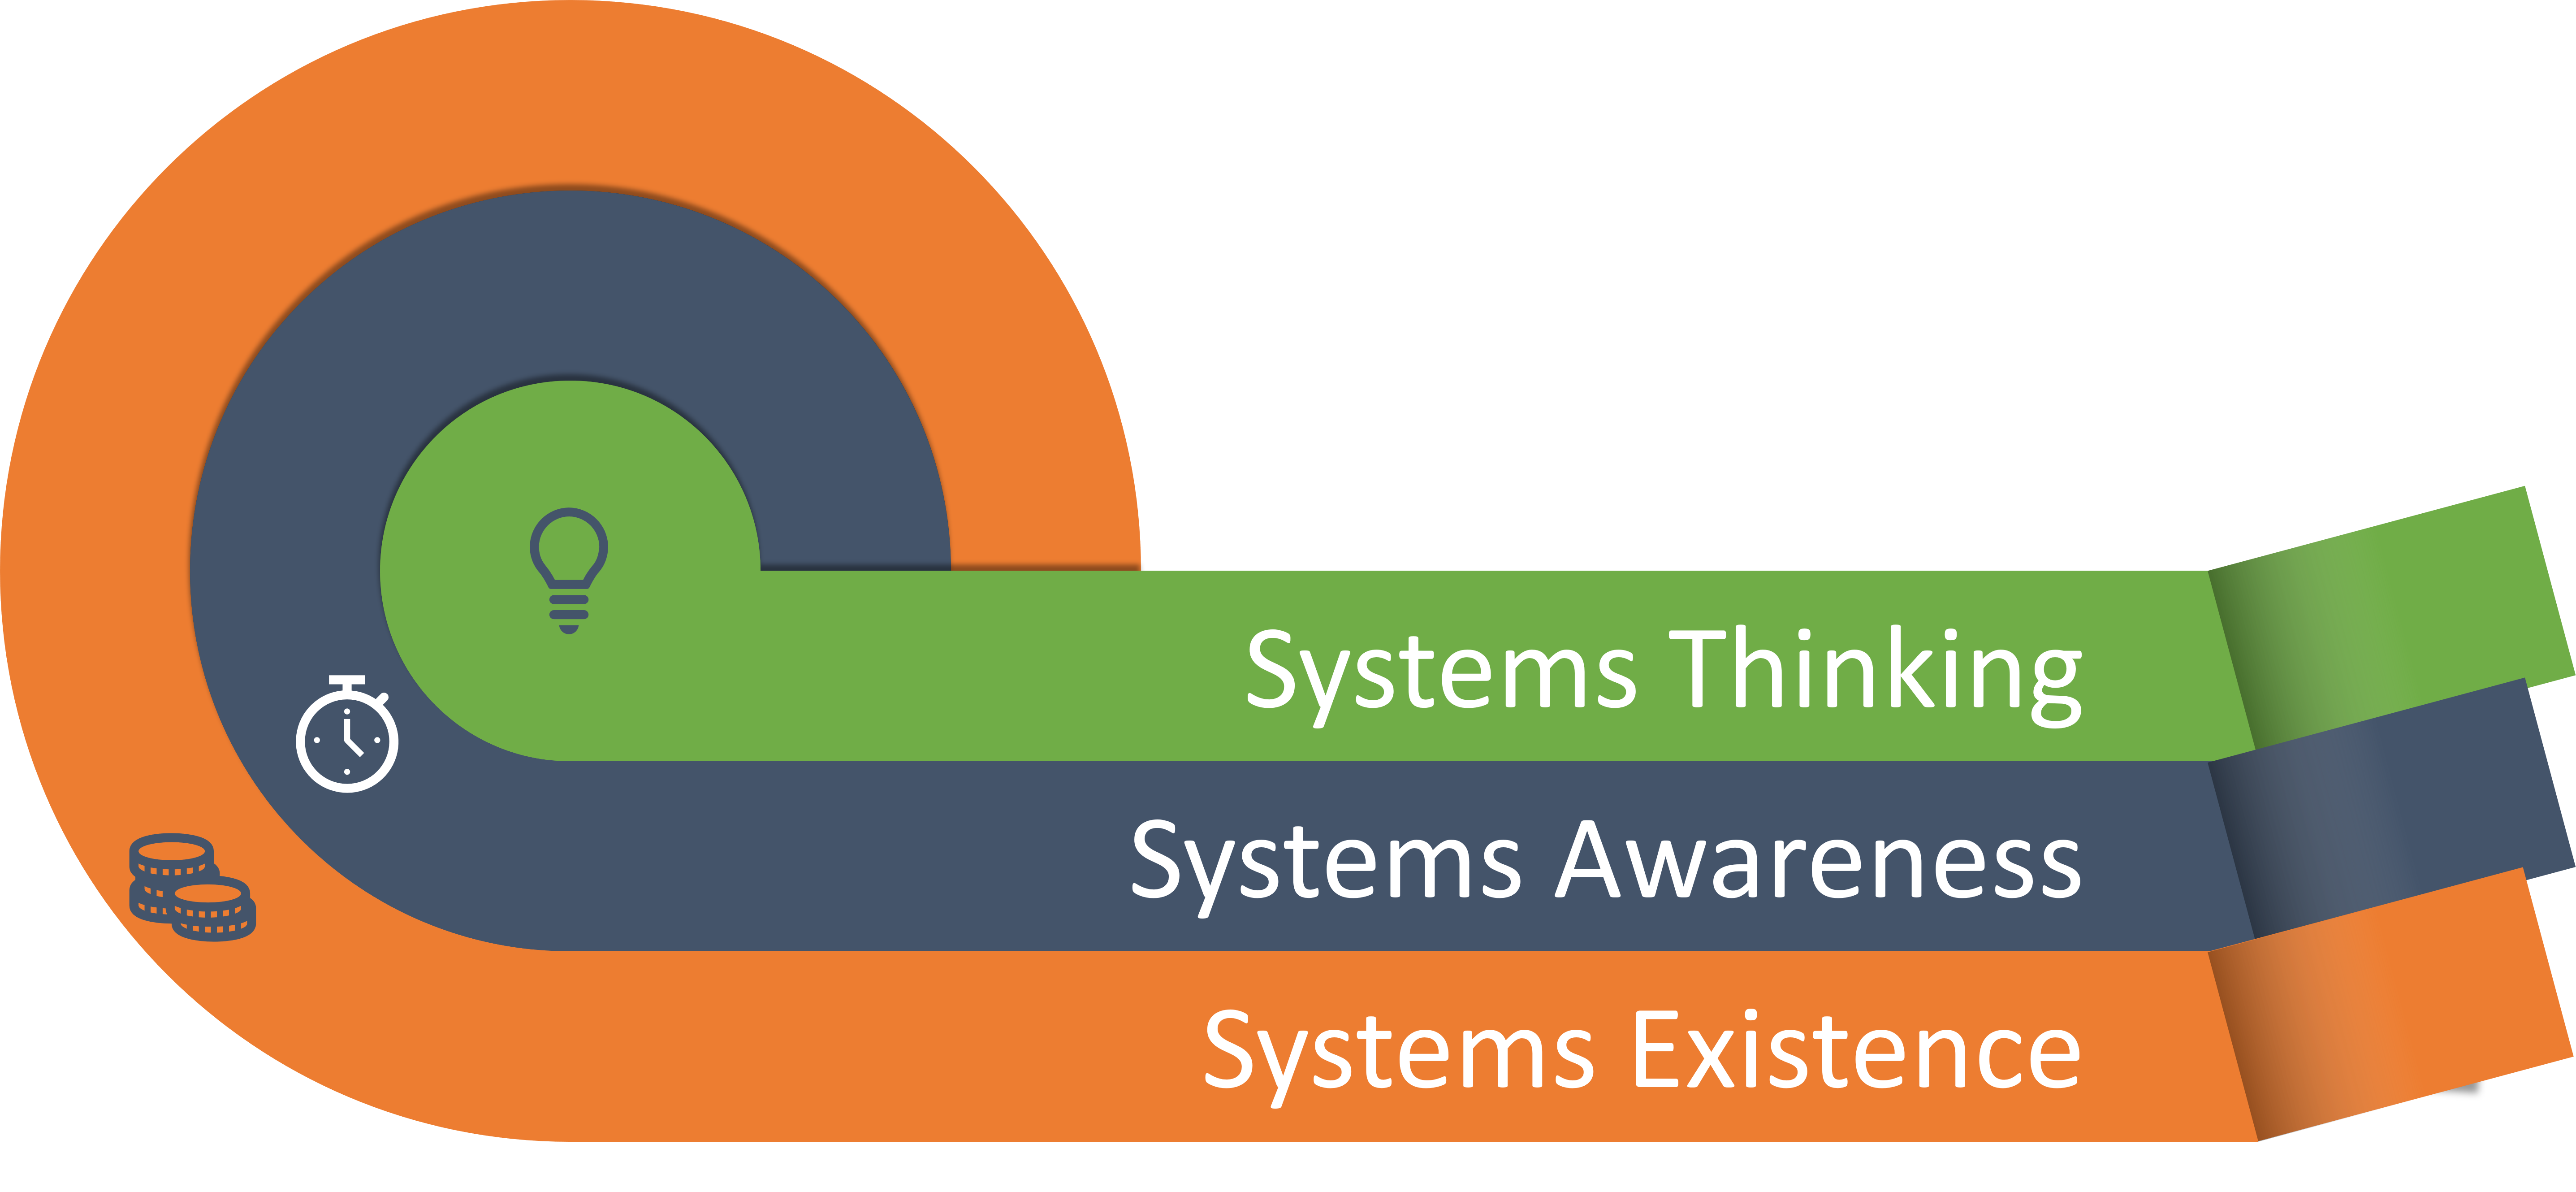
\includegraphics[width=0.9\textwidth]{systemsThinkingSnail.png}
\caption{Complete experimental setup (left) with close-up view of stage (right).}
\label{fig:systemsThinkingSnail}
\end{figure}

Figure 1.2 is conceptual in nature and self-explanatory. In science, it is argued that the only way to fully understand why a problem or element occurs and persists is to understand the parts in relation to the whole. [3] Standing in contrast to Descartes’s scientific reductionism and philosophical analysis, it proposes to view systems in a holistic manner. Consistent with systems philosophy, systems thinking concerns an understanding of a system by examining the linkages and interactions between the elements that compose the entirety of the system.

Science systems thinking attempts to illustrate that events are separated by distance and time and that small catalytic events can cause large changes in complex systems. Acknowledging that an improvement in one area of a system can adversely affect another area of the system, it promotes organizational communication at all levels to avoid the silo effect. Systems thinking techniques may be used to study any kind of system – natural, scientific, engineered, human or conceptual.

Systems thinking has been defined as an approach to problem solving, by viewing “problems” as parts of an overall system, rather than reacting to specific part, outcomes or events and potentially contributing to further development of unintended consequences. Systems thinking is not one thing but a set of habits or practices within a framework that is based on the belief that the component parts of a system can best be understood in the context of relationship with each other and with other systems, rather than in the isolation. Systems thinking focuses on cyclical rather than linear cause and effect.

\subsection{Think Globally, Act Locally}\index{Think Globally, Act Locally}

The approach adopted in this book is to recommend to globally conscious people and youth (especially STEM participants) to acquire an interest in the degree to which human designs act to modify the natural world.
\begin{enumerate}
\item More attention to design can alleviate problems revealed during operations because operational outcomes are inherent and linked to the physics of design
\item The on-line linking of individual designer’s decisions to evaluation at the system level and to stakeholder value is becoming more technically feasible. How?
\end{enumerate}

Define the system design space and partition it into the Functional domain, the Design Dependent Parameter domain, and the Optimization domain, etc.
Design Dependent Parameters (DDP’s) are suggested as the most overarching and most LINK between human designers and the human modified world. They established the design space and specific predicted and/or estimated values thereof drive design evaluation.
Design evaluation is the compass for stumbling through the design space in search of a modified world judged to be satisfactory by stakeholders.

	Add material by Kathia Laslo, PhD who directs Staybook University’s program in Leadership of Sustainable Systems . . . 
    
\subsection{Think About the End Before Beginning}\index{Think About the End Before Beginning}

From the thinking of Leonardo da Vinci
\begin{itemize}
\item WHY “To Make the World Better for People” (Retitle source here)
\item Human-made entities should be designed to satisfy human needs, wants, and objectives effectively, while minimizing system life-cycle cost as well as the intangible costs of ecological and societal impacts on the natural world
\item HOW ``Adopt and Practice Systems Thinking and Engineering''
\item A technologically based interdisciplinary process for bringing systems, products, structures, and services (human-made entities) into being
\end{itemize}

Reorient the Organization: Organization, humankind’s most important innovation, is the time-tested means for bringing human-made entities into being. While the main focus is nominally on the entities themselves, Systems Engineering embraces better strategy. Systems Engineering concentrates on what the entities do before determining what the entities are, with form following function. That is, instead of offering systems or system elements and products per se, the organizational focus should shift to designing, delivering, and sustaining functionality, a capability, or a solution.

%------------------------------------------------

\section{Relating Textbook STEA to STEM}\index{Relating Textbook STEA to STEM}

%------------------------------------------------

\section{Summary and Extensions}\index{Summary and Extensions}

Although this book focuses on the engineering of systems and on systems analysis, it would not have been intellectually prudent to begin the discussion at that level. Upon examination, it is evident that both the engineering and the analysis aspects of the focus are directed to systems. Accordingly, this chapter is devoted to helping the reader gain essential insight into systems in general, and systems thinking in particular, with orientation toward the engineering and analysis of technical systems.

System definitions, a discussion of system elements, and a high-level classification of systems provide an opening panorama. It is here that a consideration of the origin of systems provides an orientation to natural and human-made domains as an overarching dichotomy. The importance of this dichotomy cannot be overemphasized in the study and application of systems engineering and analysis. It is the suggested frame of reference for considering and understanding the interface and impact of the human-made world on the natural world and on humans. Individuals interested in obtaining an in-depth appreciation for this interface and the mitigation of environmental impacts are encouraged to read T. E. Graedel and B. R. Allenby, Industrial Ecology, 2nd ed., Prentice Hall, 2003. Also of contemporary interest is the issue of sustainability treated as part of an integrated approach to sustainable engineering by P. Stasinopoulos, M. H. Smith, K. Hargroves, and C. Desha, Whole System Design, Earthscan Publishing, 2009. These works are recommended as an extension to this chapter (as well as Chapter 16), because they illuminate and address the sensitive interface between the natural and the human-made.

This chapter is also anchored by the domains of systems science and systems engineering, beginning with the former and ending with the latter. Accordingly, it is important to recognize that at least one professional organization exists for each domain. For systems science, there is the International Society for the System Sciences (ISSS), originally named the “Society for General Systems Research.” ISSS was established at the 1956 meeting of the American Association for the Advancement of Science under the leadership of biologist Ludwig von Bertalanffy, economist Kenneth Boulding, mathematician–biologist Anatol Rapoport, neurophysiologist Ralph Gerard, psychologist James Miller, and anthropologist Margaret Mead.

The founders of the International Society for the System Sciences felt strongly that the systematic (holistic) aspect of reality was being overlooked or downgraded by the conventional disciplines, which emphasize specialization and reductionist approaches to science. They stressed the need for more general principles and theories and sought to create a professional organization that would transcend the tendency toward fragmentation in the scientific enterprise. The reader interested in exploring the field of systems science and learning more about the work of the International Society for System Sciences, may visit the ISSS website at

Most scientific and professional societies in the United States interact and collaborate with cognizant but independent honor societies. The cognizant honor society for systems engineering is the Omega Alpha Association (OAA), emerging under the motto “Think About the End Before the Beginning.” Chartered in 2006 as an international honor association, OAA has the overarching objective of advancing the systems engineering process and its professional practice in service to humankind. Among subordinate objectives are opportunities to (1) inculcate a greater appreciation within the engineering profession that every human design decision shapes the human-made world and determines its impact upon the natural world and upon people; (2) advance system design and development morphology through a better comprehension and adaptation of the da Vinci philosophy of thinking about the end before the beginning; that is, determining what designed entities are intended to do before specifying what the entities are and concentrating on the provision of functionality, capability, or a solution before designing the entities per se; and (3) encourage excellence in systems engineering education and research through collaboration with academic institutions and professional societies to evolve robust policies and procedures for recognizing superb academic programs and students. The OAA website, provides information about OAA goals and objectives, as well as the OAA vision for recognizing and advancing excellence in systems engineering, particularly in academia.

Upon completion of, the reader should have obtained essential insight into systems and systems thinking, with a focus on systems engineering and analysis. The system definitions, classifications, and concepts presented in this chapter are intended to impart a general understanding about the following:

\begin{enumerate}
\item System classifications, similarities, and dissimilarities
\item The fundamental distinction between natural and human-made systems
\item The elements of a system and the position of the system in the hierarchy of systems
\item The domain of systems science, with consideration of cybernetics, general systems theory, and systemology
\item Technology as the progenitor for the creation of technical systems, recognizing its impact on the natural world
\item The transition from the machine or industrial age to the Systems Age, with recognition of its impact upon people and society
\item System complexity and scope and the demands these factors make on engineering in the Systems Age
\item The range of contemporary definitions of systems engineering used within the profession.
\end{enumerate}

\section*{Resources for Further Exploration}
\begin{itemize}
\item \href{http://innovbfa.viabloga.com/files/Herbert_Simon___theories_of_bounded_rationality___1972.pdf}{Theories of Bounded Rationality by Herbert A. Simon}
\item \href{https://medium.com/disruptive-design/tools-for-systems-thinkers-the-6-fundamental-concepts-of-systems-thinking-379cdac3dc6a}{Tools of a Systems Thinker by Leyla Acaroglu}
\item \href{http://www.afscet.asso.fr/resSystemica/Crete02/Dyer.pdf}{Beyond Systems Design as we know it? by Gordon Dyer}
\end{itemize}

%------------------------------------------------

%% SEA CHAPTER 1 - SYSTEM SCIENCE AND ENGINEERING
% SEA Question Location in \label{sea-Chapter#-Problem#}
% ANSWERS NEED UPDATING
\begin{exercises}
    \begin{exercise}
    \label{sea-1-26}
        Describe how systems thinking differs from systems engineering.
        % What benefits could result from improving systems thinking in society?
    \end{exercise}
    \begin{solution}
        Human society is characterized by its culture. Each human culture manifests itself through the medium of technology. It takes more than a single step for society to transition from the past, to present and future technology states. A common societal response is often to make the transition and then to adopt a static pattern of behavior. A better response would be to continuously seek new but well-thought-out possibilities for advancement. Improvement in technological literacy embracing systems thinking should increase the population of individuals capable of participating in this desirable endeavor. \textbf{Reference:}
    \end{solution}
    
    \begin{exercise}
    \label{sea-1-1}
        For a system with which you are familiar, justify why it is a system according to the definition in \Cref{sec:sectors-comprising-our}.
        % Pick a system with which you are familiar and verify that it is indeed a system per the system definition given at the beginning of Section 1.1.
    \end{exercise}
    \begin{solution}
        A river system (Mississippi) is an assemblage of a watershed, tributaries, and river banks that conveys water from the continental U.S. to the Gulf of Mexico. A municipal transportation system (Chicago) is an assemblage of trains, buses, subways, etc. that transports people among many city locations. A system of organization and management (Matrix) is based on a morphology and procedure, coordinating both line and support functions. An automobile manufacturer is a combination of factories, organizations, dealerships, etc., that delivers automobiles and related support services. A home is an assemblage of land, structure, utilities, furnishings, and people that provides a supportive place to live for one or more families. \textbf{Reference:}
    \end{solution}
    
    \begin{exercise} 
    \label{sea-1-2}
        Describe the components, attributes, and relationships in the system you used in Problem \ref{sea-1-1}.
        % Name and identify the components, attributes, and relationships in the system you picked in Question 1.
    \end{exercise}
    \begin{solution}
        The major components of a home are listed in Answer 1 above. Attributes include acreage, terrain, square footage, utility capacities, styles of decorating and furnishing, personalities, and philosophies. Relationships include layout, allocation of space to people, and approaches to living together. \textbf{Reference:}
    \end{solution}
    
    \begin{exercise}
    \label{sea-1-3}
        Name any system which includes a material that transforms over the system's life cycle and identify its structural components, operating components, and flow components.
        % Pick a system that alters material and identify its structural components, operating components, and flow components.
    \end{exercise}
    \begin{solution}
        A chemica1 processing plant is composed of structural components (building, tanks, piping), operating components (pumps, valves, controls), and flow components (chemical constituents, energy, information). \textbf{Reference:}
    \end{solution}
    
    \begin{exercise} 
    \label{sea-1-4_5}
        Name any complex system and
        \begin{enumerate}[label=\alph*)]
            \item Define the hierarchy related to the system.
            \item Define the system boundaries.
        \end{enumerate}
        % Select a complex system and discuss it in terms of the hierarchy of systems.
        % Select a complex system and identify some different ways of establishing its boundaries.
    \end{exercise}
    \begin{solution}
        A dam system can be considered a complex system.
        \begin{enumerate}[label=\alph*)]
            \item todo
            \item The boundaries of a dam system can be limited to the physical dam. Alternatively, the human-modified river system, which now has a lake, can be considered a part of the dam system. The related road system, for which the dam now provides a bridge over the river, can be included. The region’s tourism service system, for which the dam system now provides an array of additional services, can be included. \textbf{Reference:}
        \end{enumerate}
    \end{solution}
    
    \begin{exercise} 
    \label{sea-1-6_7_8}
        Identify and contrast
        \begin{enumerate}[label=\alph*)]
            \item Physical versus conceptual systems.
            \item Static versus dynamic systems.
            \item Closed versus open systems.
        \end{enumerate}
        % Identify and contrast a physical and conceptual system.
        % Identify and contrast a static and a dynamic system.
        % Identify and contrast a closed and an open system.
    \end{exercise}
    \begin{solution}
        \begin{enumerate}[label=\alph*)]
            \item A physical system such as a watershed has components which manifest themselves in space and time, whereas a conceptual system such as a work breakdown structure has no physical manifestations. It is only a plan for action. Reference: Section 1.2.2 (pages 6-7).
            \item A static system such as a highway system may be contrasted with an airline system, which is a dynamic system. In the former, structure exists without activity whereas in the latter, structural components are combined with the activities of aircraft being loaded and unloaded, aircraft in flight, and controls which govern the entire operation. Reference: Section 1.2.3 (page 7).
            \item A cannon is an example of a closed system. When a cannon is fired, a one–to–one correspondence exists between the initial and final states. However, the defense contractor’s design and manufacturing organization that produced the cannon and associated projectile is an open system, with a dynamic interaction of system components. These system components must be reconfigured and adapted to cope with changing requirements. \textbf{Reference:}
        \end{enumerate}
    \end{solution}
    
    \begin{exercise} 
    \label{sea-1-15}
        For any system of the following types, name any system property
        \begin{enumerate}[label=\alph*)]
            \item Dynamic system.
            \item Steady-state system.
        \end{enumerate}
        % Give an example of a random dynamic system property and of a steady state dynamic system property.
    \end{exercise}
    \begin{solution}
        \textbf{Reference:}
    \end{solution}
    
    \begin{exercise} 
    \label{sea-1-9}
        For each of the following systems, define a unique system and describe it in terms of components, attributes, and relationships
        \begin{enumerate}[label=\alph*)]
            \item Natural system.
            \item Human-made system.
            \item Human-modified system.
        \end{enumerate}
        % Pick a natural system and describe it in terms of components, attributes, and relationships; repeat for a human-made system; repeat for a human-modified system.
    \end{exercise}
    \begin{solution}
        \begin{enumerate}[label=\alph*)]
            \item A watershed is a natural system made up of objects or components such as land, vegetation, and the watercourse; attributes such as the soil type, timber species, and the river width; and relationships such as the distribution of the attributes over the terrain. 
            \item A chemical processing plant is a human–made system with components described in Answer 3 above, attributes such as tank volume and pipe diameter, and relationships such as the flow rates and the yield of final product per energy unit utilized.
            \item A person with a pacemaker is a human-modified system with components of body parts and pacemaker parts, attributes such as body mass, diseases, attitudes, battery, controller, and electrodes, and relationships such as implantation location, rhythm, and signal strength. \textbf{Reference:}
        \end{enumerate}
    \end{solution}
    
    \begin{exercise} 
    \label{sea-1-10_11_12}
        For any Human-made system (including the system from \ref{sea-1-9})
        \begin{enumerate}[label=\alph*)]
            \item Identify the system's purpose(s) and potential metrics to present its value.
            \item Describe the system's state at any arbitrary time during operation, at least one system behavior, and an overview of the system's process.
            \item Name any two related components of the system, define the purpose of each component as it relates to the other, and the necessary attributes of the component pair such that they contribute to the purpose(s) of the entire system.
        \end{enumerate}
        % Identify the purpose(s) of the above human-made system and name some possible measures of worth.
        % For the above human-made system, describe its state at some point in time, describe one of its behaviors, and summarize its process.
        % For the above human-made system, name two components that have a relationship, identify what need each component fills for the other component, and describe how the attributes of these two components must be engineered so that the pair functions together effectively in contributing to the system’s purpose(s).
    \end{exercise}
    \begin{solution}
        \begin{enumerate}[label=\alph*)]
            \item The purposes of a chemical processing plant in a market economy are to produce one or more chemical products and possibly byproducts that can be sold at a profit while fulfilling obligations to stakeholders and the public. Measures of worth include production cost per unit volume, product quality, flexibility of product mix, benefits to stakeholders, and compatibility with society. \textbf{Reference:}
            \item During startup the state of a chemical processing plant is that pipes and vessels are filled to a certain location and empty after that location; pumps for vessels being filled are running and valves are open while other pumps are not running and valves are closed. A behavior is that when a vessel is filled, the control system turns off the pump (in a batch system) or reduces its speed (in a continuous system) and activates the next step in the process. The process is to start up, achieve the designated operational speed for each subsystem, continuously monitor the production results and make needed adjustments, and eventually shut down and clean out. \textbf{Reference:}
            \item A pump and the tank it fills have a relationship. The pump provides the material that the tank needs, while the tank provides a location where the pump can store the material it needs to deliver. The attributes of the pump must be engineered so that it can reliably move the material(s) the tank needs at an adequate rate for any given speed of overall system operation. The attributes of the tank must be engineered so that it can store the quantities of material the pump must deliver without corrosion or contamination. Thus the downstream components have the material they need to fulfill the plant’s production purpose without problems of quality or pollution. \textbf{Reference:} 
        \end{enumerate}
    \end{solution}
    
    \begin{exercise} 
    \label{sea-1-14}
        For any Human-modified system (including the system from \ref{sea-1-9}), name some positive and negative impact(s) of the modification to the natural system.
        % For a human-modified system, identify some of the ways in which the modified natural system could be degraded and some of the ways in which it could be improved.
    \end{exercise}
    \begin{solution}
        Human introduction of plant or animal species into regions where they do not naturally occur can provide the benefits of those species in the new regions, but the new species may become excessively dominant in those regions due to lack of natural enemies, crowding out or harming beneficial native species. \textbf{Reference:}
    \end{solution}
    
    \begin{exercise} 
    \label{sea-1-13}
        Give examples of each of the following
        \begin{enumerate}[label=\alph*)]
            \item First-order relationship.
            \item Second-order relationship.
            \item Redundance.
        \end{enumerate}
        % Give an example of a first-order relationship, a second-order relationship, and redundance.
    \end{exercise}
    \begin{solution}
        \begin{enumerate}[label=\alph*)]
            \item In a computer system, the power supply and system board have a first-order relationship because the system board must receive the reduced voltage produced by the power supply in order to function, and the power supply would be useless if there were no system board to perform and coordinate the computer functions. 
            \item The system board has a second-order relationship with a math coprocessor, or a video processor, or with video memory. The system board could perform the functions of these additional components, but the added components relieve the system board’s workload, thereby improving its performance.
            \item  A second power supply or a mirror image hard disk drive provide redundance, ensuring that the system board can continue receiving electrical power and the data storage function, thereby helping to assure continuation of the computer system function. \textbf{Reference:}
        \end{enumerate}
    \end{solution}
    
    \begin{exercise} 
    \label{sea-1-16}
        Name any system that operates at equilibrium and another system that degrades over time.
        % Give an example of a system that reaches equilibrium and of a system that disintegrates over time.
    \end{exercise}
    \begin{solution}
        A forest reaches equilibrium. A tree is in equilibrium until it dies, and then it disintegrates. \textbf{Reference:}
    \end{solution}
    
    \begin{exercise} 
    \label{sea-1-17}
        The United States government, for example, can be divided and described as three individual entities of the executive, legislative, and judicial branches. Create an argument for why a government of this structure should either be considered a single system or three systems.
        % Is a government with executive, legislative, and judicial branches three systems or a single system? Why?
    \end{exercise}
    \begin{solution}
        The government described is a single system because the branches thereof are functionally related. \textbf{Reference:}
    \end{solution}
    
    \begin{exercise} 
    \label{sea-1-19}
        Give any example of cybernetics and define why the example is appropriate.
        % Explain cybernetics by using an example of your choice.
    \end{exercise}
    \begin{solution}
        Cybernetics may be described and explained by considering the early mechanical version of a governor to control the revolutions per minute (RPM) of an engine. Centrifugal force, acting through a weight mechanism on the flywheel, is used to sense RPM. The outward movement of the weight against a spring acts through a link to decrease the throttle setting, thus reducing engine speed. \textbf{Reference:}
    \end{solution}
    
    \begin{exercise} 
    \label{sea-1-21}
        Do all systems at higher levels of Boulding's Hierarchy necessarily incorporate the lower levels of the hierarchy? If not, provide a specific system example.
        % Select a system at one of the higher levels in Boulding’s hierarchy and describe if it does or does not incorporate the lower levels.
    \end{exercise}
    \begin{solution}
        \textbf{Reference:}
    \end{solution}
    
    \begin{exercise} 
    \label{sea-1-22}
        Describe a novel system that may be necessary for society 50 to 100 years in the future and
        \begin{enumerate}[label=\alph*)]
            \item Define the system requirements.
            \item Define the system objectives.
        \end{enumerate}
        % Identify a societal need, define the requirements of a system that would fill that need, and define the objective(s) of that system.
    \end{exercise}
    \begin{solution}
        Efficient transportation system to the Moon and/or Mars. \textbf{Reference:}
    \end{solution}
    
    \begin{exercise} 
    \label{sea-1-25}
        For the system described in Question \ref{sea-1-22}
        \begin{enumerate}[label=\alph*)]
            \item Identify factors which led to the need for a new system.
            \item Identify other societal factors which may evolve in parallel and lead to other changes or innovations.
        \end{enumerate}
        % Name some of the factors driving technological advancement and change.
    \end{exercise}
    \begin{solution}
        \begin{enumerate}[label=\alph*)]
            \item Factors driving technological change include attempts to respond to unmet current needs and attempts to perform ongoing activities in a more efficient and effective manner, as well as social factors, political objectives, ecological concerns, and the desire for environmental sustainability. \textbf{Reference:}
            \item todo
        \end{enumerate}
    \end{solution}
    
    \begin{exercise} 
    \label{sea-1-23}
        Compare and contrast systemology and synthesis.
        % What are the similarities of systemology and synthesis?
    \end{exercise}
    \begin{solution}
        Both systemology and synthesis produce systems. Systemology produces a system of processes by which systems are brought into being and carried through the life cycle. Synthesis produces any kind of system. Synthesis is a part of systemology and also a product of systemology. \textbf{Reference:}
    \end{solution}
    
    \begin{exercise} 
    \label{sea-1-24}
        Classify a technical system.
        % What difficulty is encountered in attempting to classify technical systems?
    \end{exercise}
    \begin{solution}
        The phrase “technical system” is used to represent all types of human–made artifacts, including engineered products and processes. Classifying a technical system is generally difficult, because a technical system derives its inputs from several disciplines or fields which may be very different from one another. \textbf{Reference:}
    \end{solution}
    
    \begin{exercise} 
    \label{sea-1-27}
        Compare and contrast the attributes of the Machine (Industrial) Age and the Systems Age.
        % Identify the attributes of the Machine or Industrial Age and the Systems Age.
    \end{exercise}
    \begin{solution}
        Attributes of the Machine Age are determinism, reductionism, physical, cause and effect, and closed system thinking. The Systems Age has attributes of open systems thinking, expansionism, human–machine interfacing, automation, optimization, and goal orientation. \textbf{Reference:}
    \end{solution}
    
    \begin{exercise} 
    \label{sea-1-28}
        Identify key differences between synthetic and analytical thinking. Is one method of thinking always preferable? Why or why not?
        % Explain the difference between analytic and synthetic thinking.
    \end{exercise}
    \begin{solution}
        Analytic thinking seeks to explain the whole based on explanations of its parts. Synthetic thinking explains something in terms of its role in a larger context. \textbf{Reference:}
    \end{solution}
    
    \begin{exercise} 
    \label{sea-1-29}
        What challenges make the Systems Age unique from other periods of human evolution?
        % What are the special engineering requirements and challenges in the Systems Age?
    \end{exercise}
    \begin{solution}
        The special engineering requirements of the Systems Age are those which pertain to integration, synthesis, simulation, economic analysis, and environmental concerns, along with the necessity to bring the classical engineering disciplines to bear on the system under development through collaboration. \textbf{Reference:}
    \end{solution}
    
    \begin{exercise} 
    \label{sea-1-30}
        Compare and contrast systems engineering with other engineering disciplines.
        % What are the differences (and similarities) between systems engineering and the traditional engineering disciplines?
    \end{exercise}
    \begin{solution}
        Both systems engineering and the traditional engineering disciplines deal with technology and technical (human-made) entities. The focus of traditional engineering is on technical design of the entities in human-made systems, whereas systems engineering concentrates on what the entities are intended to do (functional design) before determining what the entities are. Traditional engineering focuses on technical performance measures, whereas systems engineering considers all requirements of the client, system owner, and/or the user group, as well as the effects on related systems. Traditional engineering focuses on designing products for their operational uses, whereas systems engineering considers all the life cycles of the systems that include its products. Traditional engineering tends to proceed from the bottom-up, whereas systems engineering favors a top-down approach. Traditional engineering favors analytic thinking while systems engineering favors synthetic thinking. Traditional engineering applies the skills of particular engineering disciplines to problems, whereas systems engineering defines problems before determining what disciplines are needed. Systems engineering provides methodologies that facilitate effective teamwork among not only the traditional engineering disciplines, but also among other technical as well as social disciplines. \textbf{Reference:}
    \end{solution}
    
    \begin{exercise} 
    \label{sea-1-32}
        Identify a system which required an interdisciplinary approach to develop \textit{or} to implement. What disciplines were required and why?
        % Give an example of a problem requiring an interdisciplinary approach and identify the needed disciplines.
    \end{exercise}
    \begin{solution}
        The problem of predicting the availability and amount of oil and natural gas from a certain geological region, which might be available to refineries and power plants in another region in future time periods, requires the disciplines of geology, petroleum engineering, regional planning, civil engineering, ecological science, transportation engineering, and economics. The validity of the prediction depends largely upon the proper utilization and interpretation of findings by the relevant disciplines and their domains of inquiry. \textbf{Reference:}
    \end{solution}
    
    \begin{exercise} 
    \label{sea-1-33}
        Identify an interdiscipline and the disciplines from which it was derived.
        % Name an interdiscipline and identify the disciplines from which it was drawn.
    \end{exercise}
    \begin{solution}
        Systems engineering is an interdiscipline (sometimes called a multidiscipline or transdiscipline) drawn mainly from the engineering disciplines, but also from mathematics, operations research, systemology, project management, and increasingly, other fields. \textbf{Reference:}
    \end{solution}
    
    \begin{exercise} 
    \label{sea-1-35_36_38}
        For the following organizations, summarize their mission statements
        \begin{enumerate}[label=\alph*)]
            \item \href{http://isss.org/}{International Society for the Systems Sciences}
            \item \href{https://www.incose.org/}{International Council on Systems Engineering}
            \item \href{https://omegalpha.org/}{Omega Alpha Association}
        \end{enumerate}
        % Go to the website for ISSS given in Section 1.7 and summarize the goal of the society.
        % Go to the website for INCOSE given in Section 1.7 and summarize the goals of the council.
        % Go to the website for OAA and compare this honor society with one that you are familiar with.
    \end{exercise}
    \begin{solution}
        \begin{enumerate}[label=\alph*)]
            \item Independent exercise. Visit http://isss.org/
            \item Independent exercise. Visit https://www.incose.org/
            \item Independent exercise. Visit https://omegalpha.org/
        \end{enumerate}
    \end{solution}
    
    \begin{exercise} 
    \label{sea-1-37}
        Explain how the goals of ISSS and INCOSE differ.
        % Contrast the goals of ISSS and INCOSE as given in Section 1.7 or on the web.
    \end{exercise}
    \begin{solution}
        Independent exercise. Refer to the solution of \ref{sea-1-35_36_38}.
    \end{solution}
\end{exercises}
% SKIPPED
% sea-1-18 Identify a system-of-systems whose analysis could yield insights not available by separately analyzing the individual systems of which it is composed.
% sea-1-20 Give a system example at any five of the levels in Boulding’s hierarchy.
% sea-1-31 Given the recommendations in Educating the Engineer of 2020, what should be added to the curriculum with which you are familiar?
% sea-1-34 Write your own (preferred) definition of systems engineering.
%%----------------------------------------------------------------------------------------
%	  CHAPTER 2
%%----------------------------------------------------------------------------------------
%\chapterimage{wireFrame.jpg} % Chapter heading image
\chapter{SCIENTIFIC THINKING AND KNOWLEDGE}\label{chap:2}

In recent decades, humans have begun to understand the underlying structure and characteristics of natural and human-made systems in a scientific way. Chapter One emphasized the human-modified world as primary evidence of the importance of drawing upon each system category.

Some system definitions and system science concepts are presented to provide a basis for the study of systems engineering and analysis. They include the definitions of system characteristics, a classification of systems into various types, consideration of the current state of systems science, and a discussion of the transition to the Systems Age. Finally, the chapter presents technology and the nature and role of engineering in the Systems Age and ends with an account of the development of systems thinking to date with extension beyond the world we know today.

\section{Human Curiosity and Inquiry}\index{Human Curiosity and Inquiry}

A major part of human nature is the curiosity of people. Curiosity leads to inquiry, and inqooint to increased understanding. “The more you learn, the more acutely aware you become of your ignorance.”

How do we know about the world in which we live – or reality, for that matter?  Where does our knowledge about it come from?  The attempt to answer these questions lead to epistemology, the branch of philosophy dealing with the origin, scope, and validity of human knowledge.

In the epistemological debate, there are two archetypal and actually diametrically opposed concepts: empiricism and rationalism. Empiricism claims that sensory experience (observation) is man’s main (or even sole) source of knowledge, which rationalism claims that his knowledge stems from human reason.

Hardly anyone would deny that there is knowledge that comes to us from sensory experience. Take, for instance, the knowledge that water freezes at zero degrees Celsius. It actually takes observation(s) to acquire such knowledge.

However, in the field of science, which formulates knowledge that applies universally, irrespective of time and place, rationalism holds that empirical knowledge gained through sensory experience doesn’t have the same validity as knowledge deduced from reasoning.
    
\subsection{Human Nature to Inquire}\index{Human Nature to Inquire}

The branches of contemporary science associated with the study of human nature include anthropology, sociology, sociobiology, and psychology, particularly evolutionary psychology, which studies sexual selection in human evolution, as well as developmental psychology. The ``nature versus nurture'' debate is a broadly inclusive and well-known instance of discussion about human nature in the natural science.

This common phrase refers to the distinguishing characteristics – including ways of thinking, feeling, and acting – which humans tend to have naturally, independently of the influence of culture. The questions of what these characteristics are, how fixed they are, and what causes them are amongst the oldest and most important questions in philosophy and science. These questions have particularly important implications in ethics, politics, and theology. This is partly because human nature can be regarded as both a source of norms of conduct of ways of life, as well as presenting obstacles or constraints on living a good life. The complex implications of such questions are also dealt with in art and literature, the question of what it is to be human.

The concept of nature as a standard by which to make judgments was a basic presupposition in Greek philosophy. Specifically, ``almost all'' classical philosophers accepted that a good human life is a life in accordance with nature. (Notions and concepts of human nature from China, Japan, or India are not taken up in the present discussion.)

On this subject, the approach of Aristotle – sometimes considered to be a teleological approach – came to be dominant by late classical and medieval times. This approach understands human nature in terms of final and formal causes. In other words, nature itself (or a nature-creating divinity) has intentions and goals, similar somehow to human intentions and goals, and one of those goals is humanity living naturally. Such understandings of human nature see this nature as an ``idea'', or ``form'' of a human. By this account, human nature really causes humans to become what they become, and so it exists somehow independently of individual humans. This in turn has sometimes been understood as also showing a special connection between human nature and divinity.

However, the existence of this invariable human nature is a subject of much historical debate, continuing into modern times. Against this idea of a fixed human nature, the relative malleability of man has been argued especially strongly in recent centuries – firstly by early modernists such as Thomas Hobbes and Jean-Jacques Rousseau. In Rousseau’s Emile, or On Education, Rousseau wrote: “We do not know what our nature permits us to be.”  Since the early 19th century, thinkers such as Hegel, Marx, Kierkegaard, Nietzsche, Sartre, structuralists, and postmodernists have also sometimes argued against a fixed or innate human nature.

Charles Darwin’s theory of evolution has changed the nature of the discussion, confirming the fact that mankind’s ancestors were not like mankind today. Still more recent scientific perspectives – such as behaviorism, determinism, and the chemical model within modern psychiatry and psychological – claim to be neutral regarding human nature. (As in much of modern science, such disciplines seek to explain with little or no recourse to metaphysical causation.)  They can be offered to explain human nature’s origins and underlying mechanisms, or to demonstrate capacities for change and diversity which would arguably violate the concept of a fixed human nature.

\subsection{How Do We Know?}\index{How Do We Know?}

The notion of ``letting the facts speak for themselves'' without taking recourse to a theory is nonsensical. Mises was aware the people’s ``reasoning may be faulty and the theory incorrect; but thinking and theorizing are not lacking in any action.''

How do we know, and how can we make sure, that we employ a correct theory?  Fortunately, in social science a satisfactory answer can be given to these questions by taking recourse to a priori theory – meaning propositions that provide true knowledge about reality, and whose truth value can be validated independent of experience.

To explain, we have to turn briefly to the Prussian philosopher Immanuel Kant (1724-1804) and his groundbreaking The Critique of Pure Reason (1781). A central outcome of what Kant called transcendental investigation in his discovery of so-called a priori synthetic judgements.
    
\subsection{\textit{A Priori} Theory}\index{\textit{A Priori} Theory}

A priori denotes a proposition (a declarative statement) expressing knowledge that is acquired prior to, or independently from, experience. In contrast, a posteriori denotes knowledge that is acquired through and on the basis of experience.

A synthetic judgment refers to knowledge that is not contained in the subject matter. An example is ``All bodies are heavy.''  Here, the predicate ``heavy'' conveys knowledge that goes beyond the mere concept of ``body'' in general. A synthetic judgment thus yields new knowledge about the subject matter.

Analytical judgments repeat what the concept of the subject matter already presupposes. An example is ``All bodies are extended.''  In order to know that bodies are extended one does not need experience, as this information is already in the concept of ``bodies.''

One would expect that analytical judgements are a priori, while synthetic judgements are posteriori. However, Kant claims that there exist a priori synthetic judgements – knowledge that neither merely repeats the meaning of the concept under review nor requires experience to say something new about the subject matter.

How can a priori synthetic judgements be identified?  According to Kant, a proposition must meet two requirements in order to qualify as an a priori synthetic judgement. First, it must not result from experience, but from reasoning. Second, it cannot be denied without causing an intellectual contradiction.

A priori theory offers an approach for reviewing, criticizing, and possibly revising commonly held theoretical explanations of historical events. When (re)viewed from point of a priori theory, what can be said about the two independent observations?

A priori theory provides true knowledge about the outer world, and the truth of knowledge derived from a priori theory can be validated independent of sensory experience.

By no means less important, a priori knowledge trumps empirical knowledge: ``A proposition of an aprioristic theory can never be refuted by experience.''

Praxeology, the a priori science of human action, and, more specifically, it’s up to now bed-developed part, economics, provides in its field a consummate interpretation of past events recorded and a consummate anticipation of the effects to be expected from future actions of a definite kind.

An a priori theorist can thus decide in advance (that is, without engaging in social experimentation, or testing, for that matter) whether or not a given action – policy measure – can bring about the promised effects.

For instance, we know a priori that issuing flat money does not create economic prosperity, that tax- or debt-financed government spending does not improve society’s material well-being, and that these measures are actually economically harmful.

A priori theory is an intellectually powerful defense against promises made by false theory and its detrimental (even disastrous) economic consequences if put into practice. Students of social sciences should therefore be increasingly encouraged to engage in a priori theory.

In his seminal book Systems Thinking, Systems Practice, Peter Checkland defined systems thinking as thinking about the world through the concept of “system.”  This involves thinking in terms of processes rather than structures, relationships rather than components, interconnections rather than separation. The focus of the inquiry is on the organization and the dynamics generated by the complex interaction of systems embedded in other systems and composed by other systems.

%------------------------------------------------

\section{Scientific Thinking in Antiquity}\index{Scientific Thinking in Antiquity}

The application of knowledge gained from the scientific method concerns prediction of the future. If X happens then Y will happen. That is the utility. Y may include probability functions.

\subsection{Classic Greek Philosophy}\index{Classic Greek Philosophy}

Philosophy in classical Greece is the ultimate origin of the western conception of the nature of a thing. According to Aristotle, the philosophical study of human nature itself originated with Socrates, who turned philosophy from study of the heavens to study of the human things.

Socrates is said to have studied the question of how a person should best live, but he left no written works. It is clear from the works of his students Plato and Xenophon, and also by what was said about him by Aristotle (Plato’s student), that Socrates was a rationalist and believed that the best life and the life most suited to human nature involved reasoning. The Socratic school was the dominant surviving influence in philosophical discussion in the Middle Ages, amongst Islamic, Christian, and Jewish philosophers.

The human soul in the works of Plato and Aristotle has a divided nature, divided in a specifically human way. One part is specifically human and rational, and divided into a part which is rational on its own, and a spirited part which can understand reason. Other parts of the soul are home to desires or passions similar to those found in animals. In both Aristotle and Plato, spiritedness (thumos) is distinguished from the other passions (epithumiai). The proper function of the ``rational'' was to rule the other parts of the soul, helped by spiritedness. By this account, using one’s reason is the best way to live, and philosophers are the highest types of human.

Aristotle – Plato’s most famous student – made some of the most famous and influential statements about human nature. In his works, apart from using a similar scheme of a divided human soul, some clear statements about human nature are made:
\begin{enumerate}
\item Man is a conjugal animal, meaning an animal which is born to couple when an adult, thus building a household (oikos) and, in more successful cases, a clan or small village still run upon patriarchal lines.
\item Man is a political animal, meaning an animal with an innate propensity to develop more complex communities the size of a city or town, with a division of labor and law-making. This type of community is different in a kind from a large family and requires the special use of human reason.
\item Man is mimetic animal. Man loves to use his imagination (and not only to make laws and run town councils). He says ``we enjoy looking at accurate likenesses of things which are themselves painful to see, obscene beasts, for instance, and corpses.''  And the ``reason why we enjoy seeing likenesses is that, as we look, we learn and infer what each is, for instance, ‘that is so and so.’''
\end{enumerate}
For Aristotle, reason is not only what is most special about humanity compared to other animals, but it is also what we were meant to achieve at our best. Much of Aristotle’s description of human nature is still influential today. However, the particular teleological idea that humans are ``meant'' or intended to be something has become much less popular in modern times.

For the Socratics, human nature, and all natures, are metaphysical concepts. Aristotle developed the standard presentation of this approach with his theory of four causes. Every living thing exhibits four aspects or ``causes'': matter, form, effect, and end. For example, an oak tree is made of plant cells (matter), grew from an acorn (effect), exhibits the nature of oak trees (form), and grows into a fully mature oak tree (end). Human nature is an example of a formal cause, according to Aristotle. Likewise, to become a fully actualized human being (including fully actualizing the mind) is our end. Aristotle (Nicomachean Ethics, Book X) suggests that the human intellect is ``smallest in bulk'' but the most significant part of the human psyche, and should be cultivated above all else. The cultivation of learning and intellectual growth of the philosopher, which is thereby also the happiest and least painful life.

Although this new realism applied to the study of human life from the beginning – for example, in Machiavelli’s works – the definitive argument for the final rejection of Aristotle was associated especially with Francis Bacon. Bacon sometimes wrote as if he accepted the traditional four causes (``It is a correct position that ``true knowledge is knowledge by causes.'' And causes again are not improperly distributed into kinds: the material, the formal, the efficient, and the final.'') but he adapted these terms and rejected one of the three:

``But of these the final cause rather corrupts than advances the sciences, except such as have to do with human action. The discovery of the formal is despaired of. The efficient and the material (as they are investigated and received, that is, as remote causes, without reference to the latent process leading to the form) are but slight and superficial, and contribute little, if anything, to true and active science.''

This line of thinking continued with Rene Descartes, whose new approach returned philosophy or science to its pre-Socratic focus upon non-human things. Thomas Hobbes, then Grammatist Vico, and David Hume all claimed to be the first to properly use a modern Baconian scientific approach to human things.

Hobbes famously followed Descartes in describing humanity as matter in motion just like machines. He also very influentially described man’s natural state (without science and artifice) as one where life would be “solitary, poor, nasty, brutish, and short.”  Following him, John Locke’s philosophy of empiricism also saw human nature as a tabula rasa. In this view, the mind is at birth a “blank slate” without rules, so data are added, and rules for processing them are formed solely by our sensory experiences.

Jean-Jacques Rousseau pushed the approach of Hobbes to an extreme and criticized it at the same time. He was a contemporary and acquaintance of Hume, writing before the French Revolution and long before Darwin and Freud. He shocked Western civilization with his Second Discourse by proposing that humans had once been solitary animals, without reason or language or communities, and had developed these things due to accidents of pre-history. (This proposal was also less famously made by Giambattista Vico.)  In other words, Rousseau argued that human nature was not only not fixed, but not even approximately fixed compared to what had been assumed before him. Humans are political, and rational, and have language now, but originally, they had none of these things. This in turn implied that living under the management of human reason might not be a happy way to live at all, and perhaps there is no ideal way to live. Rousseau is also unusual in the extent to which he took the approach of Hobbes, asserting that primitive humans were not even naturally social. A civilized human is therefore not only imbalanced and unhappy because of the mismatch between civilized life and human nature, but unlike Hobbes, Rousseau also became well known for the suggestion that primitive humans had been happier, “noble savages.”

Rousseau’s conception of human nature has been seen as the origin of many intellectual and political developments of the 19th and 20th centuries. He was an important influence upon Kant, Hegel, and Marx, and the development of German idealism, historicism, and romanticism.

What human nature did entail, according to Rousseau and the other modernists of the 17th and 18th centuries, were animal-like passions that led humanity to develop language and reasoning, and more complex communities (or communities of any kind, according to Rousseau).

In contrast to Rousseau, David Hume was a critic of the oversimplifying and systematic approach of Hobbes, Rousseau, and some others whereby, for example, all human nature is assumed to be driven by variations of selfishness. Influenced by Hutcheson and Shaftesbury, he argued against oversimplification. On the one hand, he accepted that, for many political and economic subjects, people could be assumed to be driven by such simple selfishness, and he also wrote of some of the more social aspects of ``human nature'' as something which could be destroyed, for example if people did not associate in just societies. On the other hand, he rejected what he called the ``paradox of the sceptics'', saying that no politician could have invented words like \textit{honorable}, \textit{shameful}, \textit{lovely}, \textit{odious}, \textit{noble}, and \textit{despicable}, unless there was not some natural ``original constitution of the mind.''

Hume – like Rousseau – was controversial in his own time for his modernist approach, following the example of Bacon and Hobbes, of avoiding consideration of metaphysical explanations for any type of cause and effect. He was accused to being an atheist. He wrote:

``We needn’t push our researches so far as to ask `Why do we have humanity, i.e. a fellow-feeling with others?'  It’s enough that we experience this as a force in human nature. Our examination of causes must stop somewhere.''

After Rousseau and Hume, the nature of philosophy and science changed, branching into different disciplines and approaches, and the study of human nature changed accordingly. Rousseau’s proposal that human nature is malleable became a major influence upon international revolutionary movements of various kinds, while Hume’s approach has been more typical in Anglo-Saxon countries, including the United States.

\subsection{What Man Has Built}\index{What Man Has Built}

Humanity (???) Twentieth Century, more than our ancestors, must attempt to understand the varied peoples with whom he shares an increasingly small planet. To reach this understanding he needs to know the cultures which molded other people’s outlook, the history that carried them to this point.

How to select the civilizations that must be examined in a limited series of books on the history of the world’s cultures?  That is the subject of Jaques Barzun’s introduction to the Time-Life series entitled The Great Ages of Man. Mr. Barzun, Dean of Faculties and Provost of Columbia University, is one of the pre-eminent cultural historians of this generation. He describes how the “revolution … in our conception of humanity” wrought by the emergence of “dozens of new peoples, new states, and new pasts” has made essential the realization that “nothing human is alien.”

In explaining the criteria for the selection of historic cultures examined in this series, he also suggests the path that present-day cultures may follow in the future.

At the end of this introductory booklet is a comprehensive chronological chart. This shows the meaningful relationships of great cultures the world over – in time, in place, and in the interpenetrations discussed by Dean Barzum. A number of these cultures provide the subject matter for volumes in this series. This overall chart will be found useful in connection with each book; in addition, each book includes an appropriate segment from the chart. THE EDITORS OF TIME-LIFE BOOKS (1965 Time Inc.)

%------------------------------------------------

\section{Contemporary Scientific Thinking}\index{Contemporary Scientific Thinking}

The word ``science'' is derived from the Latin word Scientia, which is knowledge based on demonstrable and reproducible data, according to the Merriam-Webster Dictionary. True to this definition, science aims for measurable results through testing and analysis. Science is based on fact, not opinion or preferences. The process of science is designed to challenge ideas through research. One important aspect of the scientific process is that it focuses only on the natural world, according to the University of California. Anything that is based on faith alone or is considered supernatural does not fit into the definition of science.

\subsection{Deductive and Inductive Reasoning}\index{Deductive and Inductive Reasoning}

During the scientific process, deductive reasoning is used to reach a logical true conclusion. Another type of reasoning, inductive, is also used. Often, deductive reasoning and inductive reasoning are confused. It is important to learn the meaning of each type of reasoning so that proper logic can be identified.

Deductive Reasoning. is a basic form of valid reasoning. Deductive reasoning, or deduction, starts out with a general statement, or hypothesis, and examines the possibilities to reach a specific, logical conclusion, according to the University of California. The scientific method uses deduction to test hypothesis and theories. ``In deductive interference, we hold a theory and based on it we make a prediction of its consequences. That is, we predict what the observations should be if the theory were correct. We go from the general – the theory – to the specific – the observations,'' said Dr. Sylvia Wassertheil-Smoller, a researcher and professor emerita at Albert Einstein College of Medicine.

In deductive reasoning, if something is true of a class of things in general, it is also true for all members of that class. For example, ``All men are mortal. Harold is a man. Therefore, Harold is mortal.''  For deductive reasoning to be sound, the hypothesis must be correct. It is assumed that the premises, ``All men are mortal'' and ``Harold is a man'' are true. Therefore, the conclusion is logical and true.

According to the University of California, deductive inference conclusions are certain provided the premises are true. It’s possible to come to a logical conclusion even if the generalization is not true. If the generalization is wrong, the conclusion may be logical, but it may also be untrue. For example, the argument, ``All bald men are grandfathers. Harold is bald. Therefore, Harold is a grandfather,'' is valid logically but it is untrue because the original statement is false.

A common form of deductive reasoning is the syllogism, in which two statements – a major premise and a minor premise – reach a logical conclusion. For example, the premise ``Every A is B'' could be followed by another premise, ``This C is A.''  Those statements would lead to the conclusion ``This C is B.'' Syllogisms are considered a good way to test deductive reasoning to make sure the argument is valid.

Inductive Rreasoning. is the opposite of deductive reasoning. Inductive reasoning makes broad generalizations from specific observations. ``In inductive inference, we go from the specific to the general. We make many observations, discern a pattern, make a generalization, and infer an explanation or a theory.'' Wassertheil-Smoller told Live Science. ``In science there is a constant interplay between inductive inference (based on observations) and deductive inference (based on theory), until we get closer and closer to the `truth', which we can only approach but not ascertain with complete certainty.''

Even if all of the premises are true in a statement, inductive reasoning allows for the conclusion to be false. Here’s an example: ``Harold is a grandfather. Harold is bald. Therefore all grandfathers are bald.''  The conclusion does not follow logically from the statements.

Inductive reasoning has its place in the scientific method. Scientists use it to form hypothesis and theories. Deductive reasoning allows them to apply the theories to specific situations.

Abductive Reasoning. Another form of scientific reasoning that doesn’t fit in with inductive or deductive reasoning is abductive. Abductive reasoning usually starts with an incomplete set of observations and proceeds to the likeliest possible explanation for the group of observations, according to Butte College. It often entails making an educated guess after observing a phenomenon for which there is no clear explanation.

Abductive reasoning is useful for forming hypotheses to be tested. Abductive reasoning is often used by doctors who make a diagnosis based on test results and by jurors who made decisions based on the evidence presented to them.

Systems Science. Systems sciences are scientific disciplines partly based on systems thinking such as chaos theory, complex systems, control theory, cybernetics, sociotechnical systems theory, systems biology, systems ecology, systems psychology and the already mentioned systems dynamics, systems engineering, and systems theory.

Systems being involves embodying a new consciousness, and expanded sense of self, a recognition that we cannot survive alone, that a future that works for humanity needs also to work for other species and the planet. It involves empathy and love for the greater human family and for all our relationships - plants and animals, earth and sky, ancestors and descendants, and the many peoples and beings that inhabit our Earth. This is the wisdom of many indigenous cultures around the world, this is part of the heritage that we have forgotten and we are in the process of recovering.

Systems being and systems living brings it all together: linking head, heart and hands. The expression of systems being is an integration of our full human capacities. It involves rationality with reverence to the mystery of life, listening beyond words, sensing with our whole being, and expressing our authentic self in every moment of our life. The journey from systems thinking to systems being is a transformative learning process of expansion of consciousness - from awareness to embodiment.

Kathia Laslo, Ph.D., directs Saybrook University’s program in Leadership of Sustainable Ssytems.
NOTE: This post is an excerpt from the plenary presentation “Beyond Systems Thinking: The role of beauty and love in the transformation of our world” by Dr. Karla Lazslo at the 55th Meeting of the International Society for the Systems Sciences at the University of Hull, U.K., on July 21, 2014.

Systems thinking is the process of understanding how things influence one another within a whole. In nature, systems thinking examples include ecosystems in which various elements such as air, water, movement, plants, and animals work together to survive or perish. In organizations, systems consist of people, structures, and processes that work together to make an organization healthy or unhealthy.

Systems thinking has been defined as an approach to problem solving, by viewing “problems” as parts of an overall system, rather than reacting to specific part, outcomes or events and potentially contributing to further development of unintended consequences. Systems thinking is not one thing but a set of habits and practices within a framework that is based on the belief that the component parts of a system can best be understood in the context of relationships with each other and with other systems, rather than in isolation. Systems thinking focuses on cyclical rather than linear cause and effect.

In science systems, it is argued that the only way to fully understand why a problem or element occurs and persists is to understand the parts in relation to the whole. Standing in contrast to Descartes’s scientific reductionism and philosophical analysis, it proposes to view systems in a holistic manner. Consistent with systems philosophy, systems thinking concerns an understanding of a system by examining the linkages and interactions between the elements that compose the entirety of the system.

Science systems thinking attempts to illustrate that events are separated by distance and time and that small catalytic events can cause large changes in complex systems. Acknowledging that an improvement in one area of a system can adversely affect another area of the system, it promotes organizational communication at all levels in order to avoid the silo effect. Systems thinking techniques may be used to study any kind of system – natural, scientific, engineered, human, or conceptual.

\subsection{The Scientific Method}\index{The Scientific Method}

The prevailing scientific thinking in Western cultures today is naturalism. It is assumed that there is no God and that the entire universe can be explained on the basis of physical realities plus time and chance. It is assumed that the laws of physics have never changed and that conditions have been uniform in the past so that recent observations can be compiled and conclusions drawn about the past by simply looking back in time. The scientific method is mostly limited to the study of measurable entities in the physical world. Results should be verifiable by others.

Figure 2.1 Here (New)

\begin{enumerate}
\item Basic Assumptions include underlying philosophy, for example is there an outside intelligence operating, or is the system closed depending only on internal known laws. Are the laws of nature constant everywhere?  Were conditions in the past the same as they are now?  What initial conditions are assumed?  Science does not and cannot take place in a vacuum – an underlying world-view or philosophy is presupposed.
\item The hypothesis is a proposed explanation for an observed phenomenon. The simpler the explanation that fits the facts, the better, known as Occam’s razor. Science assumes we live in a universe. That is, the laws of physics are the same everywhere and, furthermore, they do not vary erratically – nature is predictable, and the universe is rational.
\item If the hypothesis does not explain the known facts or the new data, it is important to carefully examine the initial conditions to if one or more of them is incorrect or suspect. Wrong assumptions a long time ago that have not been challenged cause the weight of tradition to prevail – until there are overwhelming reasons for changing the prevailing scientific paradigm.
‘Science is the only self-correcting human institution, but it is also a process that progresses only by showing itself to be wrong.’ – Alan Sandage
\item Data inputs include measurements and observations. These are systematized and subjected to statistical scrutiny whenever possible.
\item When a theory has been found that seems to the known facts, the theory is then extended into the unknown to make predictions. These predictions are then tested by seeking additional data, exceptions, or confirmations.
\item A new scientific theory or model remains in vogue until new facts are found that contradict the model or whenever a better theory comes along.
\end{enumerate}

When conducting research, scientists use the scientific method to collect measurable, empirical evidence in an experiment related to a hypothesis (often in the form of an if/then statement), the results aiming to support or contradict a theory.
The steps of the scientific method must include: 
Make an observation or observations.
Ask questions about the observations and gather information.

\begin{enumerate}
\item Form a hypothesis – a tentative description of what’s been observed, and make predictions based on that hypothesis.
\item Test the hypothesis and predictions in an experiment that can be reproduced.
\item Analyze the data and draw conclusions; accept or reject the hypothesis or modify the hypothesis if necessary.
\end{enumerate}

Reproduce the experiment until there are no discrepancies between observations and theory. ``Replication of methods and results is an essential step in the scientific method.''

Some key underpinnings to the scientific method are:
\begin{itemize}
\item The hypothesis must be testable and falsifiable, according to North Carolina State University. Falsifiable means that there must be a possible negative answer to the hypothesis.
\item Research must involve deductive reasoning and inductive reasoning. Deductive reasoning is the process of using true premises to reach a logical true conclusion while inductive reasoning takes the opposite approach.
\item An experiment should include a dependent variable (which does not change) and an independent variable (which does change).
\item An experiment should include an experimental group and a control group. The control group is what the experimental group is compared against.
\end{itemize}

Gaining new insights into the nature of systems, Hillary Sillitto, 

Several INCOSE members participated in the IFSR Conversation held April 2018 in Linz, Austria. This article is a report on some interesting results coming out of this activity. INCOSE joined the International Federation for Systems Research in 2012, interfacing through the Systems Science Working Group, and INCOSE members have participated in each Conversation since the year we joined.

One of the major activities of the International Federation for Systems Research (IFSR) is the ``conversation'' held every two years in Linz, Austria, where several teams of typically 6-8 people spend a week discussing different current issues in systems research. The format is a ``conversation'' or ``systemic inquiry'' rather than a conference, and the teams spend most of the time in their own group, exploring their specific topic and attempting to achieve new insights by integrating the different perspectives and worldviews of the different team members. 

Over forty organizations are currently IFSR members. Some are more active than others, and the Conversation this year involved people from INCOSE, ISSS, ASC (American Society of Cybernetics), the IFSR itself, and one representative from the System Dynamics Society (SDS).

The 2018 Conversation addressed four topics: ``Systems Practice'', led by members and associates of Malik Management, focused on challenges set by senior-level input from the Government of Vietnam; ``What is Systems Science?'', led by Gary Smith of INCOSE with a team of INCOSE and IFSR members; ``Active and Healthy Aging'', using Beer’s Viable System Model and a subset of Len Troncale’s System Processes as reference models to understand the challenges facing older members of our communities; and ``Data Driven SE Approaches'', led by Ed Carroll of INCOSE and Sandia Labs, with several INCOSE members, the SDS representative, and several others from Sandia.

Ed Carroll’s team considered the problem of integrating the heterogeneous model types used by different engineering domains, discussed issues such as how to get people to trust models, identified the need for Systems Engineering to shift from a process-centric to an information-centric perspective if MBSE is to succeed, and were inspired by the ``agile manifesto'' to start working up an analogous ``MBSE manifesto''. Their outbrief advocated viewing the model as being the focus, rather than the process of creating it. Others pointed out the tension between this perspective and the verified success of ``shared model building'' as a method for engaging stakeholders, and developing their trust in the model. Someone suggested that ``no-one understands a model except the people who created it''. I look forward to seeing the MBSE manifesto and to the discussions it will undoubtedly provoke about the culture change required in the SE community to take full advantage of the model driven approach while being fully aware of its limitations: not all systems are deterministic, some systems ``have a mind of their own''; and for these, modeling can indicate the range of possible future trajectories but not the precise one that will be followed.

Gary Smith’s team discussed ``What is systems science''. Gary smith made a plausible argument that in historical terms, Systems Science is now where chemistry was before the Periodic Table of the elements - lots of phenomena have been described, many of them understood as individual phenomena, but this knowledge is not yet integrated around a single foundational structure. Further, the current systems science literature in most cases does not clearly distinguish between fundamental ingredients of all systems (think electrons, protons and neutrons), properties of all systems (think properties of atoms and elements due to the electron orbitals) and properties that can be synthesised with combinations of different ``elemental types'' of system – think compounds, crystals, alloys, etc. Most Systems Science literature also does not clearly distinguish between ``how people perceive and interact with systems'', and fundamental ``properties of systems in the natural world''. (Robert Rosen’s book Anticipatory Systems is a notable exception.) We spent the week exploring whether existing systems science knowledge could usefully be organised in this sort of structure, and concluded that it could, and that such a structure offers promise in terms of integrating the seven different worldviews on system we have identified within the INCOSE community. Also, we identified an eighth worldview about systems, that ``systemness'' might be a fundamental organising principle of nature. Our output and subsequent reflections are being posted to a website which will progressively be opened up to SSWG members and then more widely as the content matures.

I participated in the “What is systems science?” team, and also represented INCOSE at the IFSR Board Meeting on the Friday afternoon at the end of the Conversation. The notable points of the Board Meeting were: our old friend Gerhard Chroust stands down as IFSR’s Secretary General after 27 years of service; Gary Metcalf, Jennifer Wilby and Mary Edson also finished their terms of service; new faces join the Board, and Ray Ison takes over from Mary as president; George Mobus has taken over as general Editor of the IFSR book series; and the System Dynamics Society’s membership application was approved. Hillary Sillitto, ESEP, INCOSE Fellow

%------------------------------------------------

\section{Science and Systems Science}\index{Science and Systems Science}

The significant accumulation of scientific knowledge, which began in the eighteenth century and rapidly expanded in the twentieth, made it necessary to classify what was discovered into scientific disciplines. Science began its separation from philosophy almost two centuries ago. It then proliferated into more than 100 distinct disciplines. A relatively recent unifying development is the idea that systems have general characteristics, independent of the area of science to which they belong. In this section, the evolution of a science of systems is presented through an examination of cybernetics, general systems theory, and systemology.

\subsection{General Systems Theory}\index{General Systems Theory}

An even broader unifying concept than cybernetic evolved during the late 1940’s. It was the idea that basic principle common to all systems could be found that go beyond the concept of control and self-regulation. A unifying principle for science and a common ground for interdisciplinary relationships needed in the study of complex systems were being sought. Ludwig von Bertalanffy used the phrase general systems theory around 1950 to describe this endeavor. A related contribution was made by Kenneth Boulding.

General systems theory is concerned with developing a systematic framework for describing general relationships in the natural and the human-made world. The need for a general theory of systems arises out of the problem of communication among various disciplines. Although the scientific method brings similarity between the methods of approach, the results are often difficult to communicate across disciplinary boundaries. Concepts and hypotheses formulated in one area seldom carry over to another, where they could lead to significant forward progress.

One approach to an orderly framework is the structuring of a hierarchy of levels of complexity for individual systems studied in the various fields of inquiry. A hierarchy of levels can lead to a systematic approach to systems that has broad application. Boulding suggested such a hierarchy. It begins with the simplest level and proceeds to increasingly complex levels that usually incorporate the capabilities of all the previous levels, summarized approximately as follows:

\begin{enumerate}
\item The level of static structure or frameworks, ranging from the pattern of the atom to the anatomy of an animal to a map of the earth to the geography of the universe.
\item The level of the simple dynamic system, or clockworks, adding predetermined, necessary motions, such as the pulley, the steam engine, and the solar system.
\item The level of the thermostat or cybernetic system, adding the transmission and interpretation of information.
\item The level of the cell, the open system where life begins to be evident, adding self-maintenance of structure in the midst of a through put of material.
\item The level of the plant, adding a genetic-societal structure with differentiated and mutually dependent parts, “blueprinted” growth, and primitive information receptors.
\item The level of the animal, adding mobility, teleological behavior, and self-awareness using specialized information receptors, a nervous system, and a brain with a knowledge structure.
\item The level of the human, adding self-consciousness, the ability to produce, absorb, and interpret symbols; and understanding of time, relationship, and history.
\item The level of social organization, adding roles, communication channels, the content and meaning of messages, value systems, transcription of image into historical record, art, music, poetry, and complex human emotion.
\item The level of the transcendental system, adding the ultimates and absolutes and unknowables.
\end{enumerate}

The first level in Boulding’s hierarchy is the most pervasive. Static systems are everywhere, and this category provides a basis for analysis and synthesis of systems at higher levels. Dynamic systems with predetermined outcomes are predominant in the natural sciences. At higher levels, cybernetic models are available, mostly in closed-loop form. Open systems are currently receiving scientific attention, but modeling difficulties arise regarding their self-regulating properties. Beyond this level, there is little systematic knowledge available. However, general systems theory provides science with a useful framework within which each specialized discipline may contribute. It allows scientists to compare concepts and similar findings, with its greatest benefit being that of communication across disciplines.

\subsection{Systemology and Synthesis}\index{Systemology and Synthesis}

The science of systems or their information is called systemology. Problems and problem complexes faced by humankind are not organized along disciplinary lines. A new organization of scientific and professional effort based on the common attributes and characteristics of problems will likely accelerate beneficial progress. As systems science is promulgated by the formation and acceptance of interdisciplines, humankind will benefit from systemology and systems thinking.

Disciplines in science and the humanities developed largely by what society permitted scientists and humanists to investigate. Areas that provided the least challenge to cultural, social, and moral beliefs were given priority. The survival of science was also of concern in the progress of certain disciplines. However, recent developments have added to the acceptance of a scientific approach in most areas. Much credit for this can be given to the recent respectability of interdisciplinary inquiry. One of the most important contributions of systemology is that it offers a single vocabulary and a unified set of concepts applicable to many types of systems.

During the 1940s, scientists of established reputation in their respective fields accepted the challenge of attempting to understand a number of common processes in military operations. Their team effort was called operations research, and the focus of their attention was the optimization of operational military systems. After the war, this interdisciplinary area began to take on the attributes of a discipline and a profession. Today a body of systematic knowledge exists for both military and commercial operations. But operations research is not the only science of systems available today. Cybernetics, general systems research, organizational and policy sciences, management science, and the information sciences are others.

Formation of interdisciplines began in the middle of the last century and has brough about an evolutionary synthesis of knowledge. This has occurred not only within science but also between science and technology and between science and the humanities. The forward progress of systemology in the study of large-scale complex systems requires a synthesis of science and the humanities as well as a synthesis of science and technology. Synthesis, sometimes referred to as an interdisciplinary discipline, is the central activity of people often considered to be synthesists.

The science community must build public understanding of and appreciation for science and evidence-based thinking. We must show that evidence-based thinking leads to more reliable policies to create jobs, maintain a healthy environment and improve teaching.

With more than 120,000 members across the world, the American Association for the Advancement of Science is uniquely positioned to bring together voices and ideas from a diverse range of disciplines and backgrounds to lead the charge. But we need your help.

With your support, we will expand our efforts to speak up and draw people — the public and policymakers — to the idea that science is relevant to their lives and can inform their decisions. We will provide training, tools, and resources for scientists to communicate their research and find opportunities to connect with loc

\subsection{Emergence}\index{Emergence}

\subsection{Ethical Principles From the Basics of Science}\index{Ethical Principles From the Basics of Science}

The principles that form the basis of every rational discussion, that is, of every discussion in the search for truth, are in the main ethical principles. I should like to state three such principles:

\begin{enumerate}
\item The principle of fallibility: perhaps I am wrong and perhaps you are right. But we could easily both be wrong.
\item The principle of rational discussion: we want to try, as impersonally as possible, to weight up our reasons for and against a theory; a theory that is definite and criticizable.
\item The principle of approximation to the truth: we can nearly always come closer to the truth in a discussion which avoids personal attacks. It can help us to achieve a better understanding; even in those cases where we do not reach an agreement.
\end{enumerate}

It is worth noting that these three principles are both epistemological and ethical principles. For they imply, among other things, toleration: if I hope to learn from you, and I want to learn in the interest of truth, then I have not only to tolerate you but also to recognize you as a potential equal; the potential unity and willingness to discuss matters rationally. Of importance also is the principle that we can learn much from a discussion, even when it does not lead to agreement: a discussion can help us by shedding light upon some of our errors.

You raise an interesting question, one which has caused argument and confusion over many years. Considering the advanced state of systems engineering, systems thinking, etc., this state of affairs might be considered curious, at the very least.

The problem with defining “systems” is that various disciplines perceive “system” from their own perspectives, and may not always define “system” in an entirely general way. For instance, engineers today often describe complicated artefacts as systems, whereas 20-30 years ago they described them as ‘equipments.’  The artefacts haven’t changed, but somehow the soubriquet ‘system’ has taken over, whether appropriate or not.

Aerospace engineers might describe an aircraft as a system, or even a system of systems, while others might describe the aircraft as a sophisticated artefact, a tool, for the use of a pilot and crew. Together, aircraft and crew comprise a sociotechnical system. Why?  Because only when together, man and machine, is the flying machine complete. Neither man nor machine can fly without the other.

So, an important element of any definition of ‘system’ is the notion of completeness. A system is a complete something that, usually, performs some function(s). A gambling system is a means and method for winning at gambling, but it is only a system if all the moves, all the tactics, are in place. If only one is absent – no system.

Another aspect of ‘system’ in general is organization. By definition, a system is organized. It is not enough for a system to comprise many parts: these parts have to be interconnected, interacting and organized. A system’s “degree of organization” can be measured as entropy. The lower the entropy of a system, the more of its internal energy can be converted for useful external work. (Second Law of Thermodynamics)

Some systems are purposeful: humans as systems can be purposeful. Are all systems purposeful? Apparently not. The solar system is organized, low configuration entropy, etc. – we cannot avow that it is complete – yet it appears to have no explicit purpose, outside of the transcendental, that is. So, purpose need not form part of any definition … nor does the solar system perform any notable function: it just `is.’ So, is function essential?

Within systems there are observed to be levels of organization. For living things, the smallest element that can be described as living in the cell. All living things are made from cells. However, the cells are organized, grouped into tissues; tissues into organs; organs into organ systems; organ systems into organisms (species); species into populations; populations into communities, communities into ecosystem, ecosystems into biomes; biomes into the biosphere. So, an empiricist might say, with some justification, that the definition of “system” places it necessarily in such a hierarchy of organization.

Reductionists, OTOH, seek to explain high-level phenomena in more fundamental, low level explanations. Some argue that the relation between high and low – supervenience - may not allow for reduction. High level properties may be irreducible and may represent new, emergent properties that are more than the sum of their parts. The simple, limited behavior of individual ants results in the sophisticated organization of a colony.

So, another aspect of `system’ is that some systems may exhibit emergent properties, properties/behaviors of the whole that are not evident in the properties/behaviors of the parts. Some pundits seek to divide emergence into `weak’ and `strong,’ where weak is predictable, calculable, and not, therefore, entirely justifiable as emergence. Should emergence appear in the definition of `system?’  Possibly, if only because many natural systems do exhibit emergence (e.g., the Hymenoptera), and some (complex?) manmade systems also exhibit emergence.

Lastly, a system has be open, i.e., it exchanges energy, information and substance with other systems and with its environment. Were a system truly closed, we would be unaware of it.

%------------------------------------------------

\section{Scientific Theory and Laws}\index{Scientific Theory and Laws}

\subsection{What is Scientific Theory?}\index{What is Scientific Theory?}

Imagine for a moment that you are omniscient. Endowed with such knowledge, you would completely understand how the world ``works.''  You would completely understand how light works, how molecules and atoms work, how genetics work, how tectonic plates work, and how the universe came into existence. There would be nothing about the social or natural worlds that you would not understand in its entirety.

Where you endowed with such omniscience, you would have no use whatsoever for ``science.''  You would have no need to study the world in a patient and systematic way; because you would already possess all the knowledge about the world that ``science'' could ever hope to yield. Science would not only bore you to tears; it would appear to be an imperfect and dreadfully tedious means to arrive at the knowledge you already possess.

Unfortunately, however, no human being possesses omniscience. We are born into the world without knowledge about how light works, how tectonic plates work, how atom work, and how the universe came into existence. We also lack perfect knowledge about how capitalism and socialism work, how democracy and monarchy work, and how price controls work.

Our uncertainty about how the social and natural worlds work restricts our ability to act. Our uncertainty about how tectonic plates work restricts our ability to predict and control earthquakes. Our uncertainty about how light works restricts our ability to harness it for our own purposes. And our uncertainty about how monarchy and democracy work restricts our ability to construct political and economic systems that are best suited to our nature. This list could be extended ad infinitum.

We are not without means to overcome our uncertainty about how the world works, however. We are not, like the brute animals, doomed to struggle for our existence in a world that we will never understand or be able to harness for our own purposes. We have reason and memory at our disposal, which, with the aid of our senses, allow us to examine the world and learn how its elements ``work.'' These fantastic mental abilities afford us the means to investigate the world in the hope of overcoming at least a small part of our natural ignorance and uncertainty.

Our fantastic mental abilities do not, however, automatically yield to us infallible knowledge about how the world works. We can misinterpret what is going on, and we can reason unsoundly. Our senses can fail us, and our thinking can become clouded, biased, or myopic. In addition, the world we seek to understand is so fantastically large and complicated, and our time so very scarce, that each of us is severely limited in the amount of knowledge we can individually acquire about how the world works.

Hence, only by working with an learning from other men can we as individual hope to learn more than a tiny fraction about how the world works. By working with and learning from other men, we can take advantage of an intellectual division of labor that allows individuals to investigate very specific aspects of the world and then share the fruits of their investigations with the rest of humanity. This specialization and exchange of ideas allows men to economize their scarce time, learn more about the world than they otherwise could as isolated individual, and serves as a check on the fallible reasoning of each individual.

The concept of ``science'' in the Western world has been to connect a community of individuals who are committed to study the world in a specialized, systematic, and intersubjective verifiable way. Ideally, this scientific community accumulates knowledge about how the world works as individuals learn from the specialized investigations of their colleagues and build on them, and as the scientific community critiques and refines their theories through time.

The process by which the scientific community investigates the world is not a magic or automatic path to enlightenment or omniscience, however. The theories that are fashionable in the scientific community at any specific moment may or may not accurately describe the actual working of the world. Communities of individual scholars, like the individual scholars themselves, can fall victim to intellectual error. They can misinterpret what is going on, and they can reason unsoundly. Their senses can fail them, and their thinking can become clouded, biased, or myopic.

The critical and inexorable problem that the community of scholars faces, therefore, is knowing whether the theories it currently embraces accurately and completely describe the workings of the world. This uncertainty about the accuracy of their scientific theories stems, once again, from the fact that no member of the scientific community is omniscient. No member of the scientific community is in a position to say with certainty that any theory does or does not accurately describe the workings of the world.

If even one member of the scientific community were omniscient, it would be possible to appeal to that member as an objective assessor of scientific theories. In that case, the omniscient assessor would not trouble himself with describing the world using the clumsy word ``theory,'' however. He would say ``the world works thusly,'' or ``the world does not work thusly.'' If such a person existed, moreover, the practice of ``science'' would cease altogether, because certain knowledge about the world could be obtained from the omniscience person without the need to tediously and imperfectly study the world ``scientifically.''

Because the scientific community does not count omniscient members among its number, its members have developed a ``scientific method'' to try to deal with their uncertainty about their theories. The ``scientific method,'' which consists of developing hypotheses and ``testing'' those hypotheses against empirical experience, does not provide the scientific community with certain knowledge, however. It merely serves a rather low hurdle that assists in weeding out what most scientists would consider implausible, unverifiable, and silly theories.

A theory’s ability to clear this low hurdle by no means can be interpreted as ``verifying'' a theory, or ``proving'' its truth, however, because alternative theories could always be imagined that would also be consistent with the empirical ``facts.''  The scientific method does not provide the scientific community with a means to determine which theory, if any, out of the limitless set of alternative theories that could be dreamed up to explain the same empirical phenomena is ``correct.''  Nor does the scientific method provide the scientific community with a means to know for certain that its members are not misinterpreting the empirical evidence. Only an omniscient being could know these things for certain.

Because empirical evidence doesn’t not ``speak for itself,'' and because scientists are not omniscient (and thus cannot know if they are ``correctly'' interpreting empirical evidence), scientists can never know for certain if their theories correctly describe physical reality. This means that any theory that relies on the interpretation of empirical evidence can never be more than a subjective statement of belief about how a part of the world works, based on some empirical evidence.

This definition is unavoidable, because no scientist is in an omniscient position to know for certain whether he has interpreted empirical evidence correctly, or whether his theory is the ``correct'' one out of the infinite set of alternative theories that could be imagined to explain a given phenomenon.

This is not to say that scientific theories rely on the interpretation of empirical evidence are useless or meaningless, simply because they are subjective statements of belief. Nor does it imply that all empirically derived scientific theories are equally plausible, or that they all must be deemed “equal” in some other way, simply because they are all subjective statements of belief about how the world works. On the contrary, a theory that relies on empirical evidence is nothing more than an ``expert opinion'' about how a part of the world works, but it can nevertheless be useful - sometimes amazingly useful, in fact – even when it is known to be ``incorrect'' in some respects (e.g., Newtonian physics). Moreover, individual are free to evaluate the plausibility of scientific theories on their own, which means that they are free to accord some empirical theories more plausibility than others.

The fact that scientific theories are subjective statements of belief does mean, however, that the scientist who claims that his empirically derived theory is a ``fact'' or ``undeniably certain'' does not understand the limitations of his method. He is deluding himself – and anyone else who believes his claims – if he thinks he is able to ``prove'' his empirically derived theory to be ``irrefutably true.''  Only an omniscient being could possibly know for certain that a specific theory out of the infinite set of alternative theories that could be imagined to explain a given phenomenon is ``correct.''  But, again, an omniscient being would not bother with the clumsy and inefficient methods of science. He would merely say, ``the world works thusly,'' or ``the world does not work thusly.''  He certainly would not bother ``testing'' his ideas against empirical experience, because he would already know the outcome. Hence, the fact that the scientist bother to ``test'' his theories and hypotheses reveals his lack of omniscience, and it also reveals, a fortiori, his inability to know for certain whether he is interpreting empirical evidence ``correctly.''

In order to move beyond making subjective statements of belief about how parts of the world work the scientist would either need to become omniscient himself or consult someone who is omniscient, or else he would need to move beyond gathering and interpreting empirical evidence. Because the former options are, presumably, not open to him, the scientist’s only viable option is to discover “facts” about the world, or parts of the world, that cannot possibly be thought to be false, and which are not open to misinterpretation. In other words, the scientist would have to transform himself from an empiricist into a ``rationalist'' who was concerned to discover fundamental truths about the world (i.e., a priori truths about the world) and elucidate them by means of a deductive and rationalistic method. Only then would the scientist be in a position to say that he has found “facts” about parts of the world that are ``indisputably true.''

By dogmatically endorsing the ``scientific method'' as the only means to acquire knowledge about the world, the empirically minded scientist tacitly admits that it is possible to discover fundamental truths about the world without going out and ``testing'' them. For, the proposition ``all hypotheses and theories must be `tested’ against empirical experience'' purports to be objectively and universally true, yet the proposition itself has not and can never be ``tested.''  Therefore, the proposition is self-contradictory and thus false, a fact that establishes that it is indeed possible to discover irrefutable and demonstrable truths about the world without going out and testing them.

Thus, absolute certainty in science cannot be acquired by means of the “scientific method” and the collection and interpretation of empirical evidence. For beings that lack omniscience, collection and interpretation of empirical evidence can only yield imperfect and subjective beliefs about how the world “works.”  Instead, absolute certainly in science can only be acquired by discovering propositions about the world that can be known to be true a priori – propositions that cannot be thought to be false.

This observation, in a nutshell, forms the foundation and is the great strength of the Austrian School of economics, which stands virtually alone in the contemporary would as a bastion for thinkers who are unsatisfied with imperfect and subjective approaches to science.

System thinking is not enough. We must also engage in systems feeling and making. We must start during conceptual design and continue through the multiple years of integration and maintenance of operational systems.

SysML helps us make the evidence that system thinking has occurred. SysML must be augmented by ways of communicating intended system feeling, particularly for systems that include humans as active components. Example attributes might be engages, influences, inspires, learns, etc. as well as trusted, trustworthy, alert, etc.

While designing a system model we must ensure that these necessary and sufficient emotions and judgements are in play and evolving in the right direction(s).

An extension to SysML is not likely, rather associated stories and a set of key metrics may be appropriate. Azad Madni and others such as IDEO and other design laboratories have shown us examples of such stories. Tom Love champions performing conceptual design sans words, a flow of cartoons only.

How shall we evolve an ontology for the Feeling aspect of systems as an adjunct to SysML, particularly for highly autonomous systems that emulate human emotions? Jack.

\subsection{Acknowledging Scientific Risk}\index{Acknowledging Scientific Risk}

The knowledge that is built buy science is always open to question and revision. No scientific idea is ever once-and-for-all ``proved.''  Why not?  Well, science is constantly seeking new evidence, which could reveal problems with our current understandings. Ideas that we fully accept today may be rejected or modified considering new evidence discovered tomorrow. For example, up until 1938, paleontologists accepted the idea that coelacanths (an ancient fish) went extinct at the time that they last appear in the fossil record – about 80 million years ago. But that year, a live coelacanth was discovered off the coast of South Africa, causing scientists to revise their ideas and begin to investigate how this animal survives in the deep sea.

Even though they are subject to change, scientific ideas are reliable. The ideas that have gained scientific acceptance have done so because they are supported by many lines of evidence. These scientific explanations continually generate expectations that hold true, allowing us to figure out how entities in the natural world are likely to behave (e.g., how likely it is that a child will inherit a particular genetic disease) and how we can harness that understanding to solve problems (e.g., how electricity, wire, glass, and various compounds can be fashioned into a working light bulb). For example, scientific understandings of motion and gases allow us to build airplanes that reliably get us from one airport to the next. Though the knowledge used to design airplanes is technically provisional, time and time again, that knowledge has allowed us to produce airplanes that fly. We have good reason to trust scientific ideas: they work!

Systems science - systemology (Greco. Systema, logos) or systems theory is an interdisciplinary field that studies the nature of systems - from simple to complex - in nature, society, and science itself. The field aims to develop interdisciplinary foundations that are applicable in a variety of areas, such as engineering, biology, medicine, and social sciences.

Systems science covers formal sciences such as complex systems, cybernetics, dynamical systems theory, and systems theory, and applications in the field of the natural and social sciences and engineering, such a control theory, operations research, social systems theory, systems biology, system dynamics, human factors, systems ecology, systems engineering and systems psychology. Themes commonly stressed in system science are (a) holistic view, (b) interaction between a system and its embedding environment, and (c)complex (often subtle) trajectories of dynamic behavior that sometimes are stable (and thus reinforcing), while at various `boundary conditions’ can become wildly unstable (and thus destructive). Concerns about Earth-scale biosphere/geosphere dynamics is an example of the nature of problems in which systems science seeks to contribute meaningful insights.

Since the emergence of general systems research in the 1950s, systems thinking and systems science have developed into many theoretical frameworks.
Systems notes of Henk Bikker, TU Delft, 1991

A theory is almost never proven, though a few theories do become scientific laws. One example would be the laws of conservation of energy, which is the first law of thermodynamics. Dr. Linda Boland, a neurobiologist and chairperson of the biology department at the University of Richmond, Virginia told Live Science that this is her favorite scientific law. ``This is one that guides much of my research on cellular electrical activity and it states that energy cannot be created nor destroyed, only changed in form. This law continually reminds me of the many forms of energy,'' she said.

Laws are generally considered to be without exception, though some laws have been modified over time after further testing found discrepancies. This does not mean theories are not meaningful. For a hypothesis to become a theory, rigorous testing must occur, typically across multiple disciplines by separate groups of scientists. Saying something is ``just a theory'' is a layperson’s term that has no relationship to science. To most people a theory is a hunch. In science a theory is the framework for observations and facts, Jaime Tanner, a professor of biology at Marlboro College, told Life Science.

Debate on whether `scientific consensus’ is to be given special weight seems to turn on the two-sides of the injunction from Richard Feynman:

“When someone says science teaches such and such, he is using the word incorrectly. Science doesn’t teach it; experience teaches it. If they say to you science has shown such and such, you might ask, “How does science show it – how did the scientists find out – how, what, where?”  Not science has shown, but this experiment, this effect, has shown. And you have as much right as anyone else, upon hearing about the experiments (but we must listen to all the evidence), to judge whether a reusable conclusion has been arrived at.
    • (Feynman, “The Pleasure of Finding things out”, page 187, emphasis added)
    
Is there any dispute that both aspects are required for the integrity of the scientific process?

\begin{enumerate}
\item Everyone has the right to judge for themselves whether `a reusable conclusion’ has been arrived at, \textit{but}
\item This must be done after listening to all the evidence, including what, how, and where scientists obtained the evidence
\end{enumerate}

I have not studied this topic in detail, but from a common-sense point of view, it does seem that many people (groups) want to declare their beliefs to be true, with these beliefs often coming from what they wish to be true based on ulterior motives or to conform with a specific narrative.

Kant wins. Marx wins. Everything has become politicized. Death of reason and dialogue. Victory to mindless rhetoric. Say it enough and people will believe it is true.

A person’s right to believe as he/she wishes does not imply an obligation on anyone else to accept that belief, no matter how many people choose to accept it. A group claiming it has consensus on a viewpoint cannot claim truth any more than a jury declaring “not guilty” proves the defendant is innocent of the act. A claim of consensus is not a form of higher or moral authority over others. It is not an act of reason. It is an act of intellectual treason.

Remember, it was consensus that all swans were white. It was consensus that the heavens revolved around the Earth, while simultaneously the world was flat. Until, of course, that those pesky non-believers and intellectual saboteurs revealed the errors by having the guts to find black swans and circumnavigate the Earth.

My lay viewpoint is that we would do well to eliminate the concept of “consensus” from our consciousness when speaking of science. Consensus does not imply truth.

We might also wish to recall Warfield’s definition of Clan-Think when touting consensus.

This makes interesting demands on education.

RE: “the practice of science has achieved considerable success by setting goals of sharing information to enable independent replication, debate, and testing of predictions – that is, valuing objective evidence over personal opinion or ideology or theology.”

Is there some other mode of the practice of science  that does not require independent replication, debate, and testing of predictions?

I ask this because it seems you are saying that humans are also practicing science when a sufficient number simply agree on some assertion without performing independent replication, debate, and testing.

Are you saying that replication, debate, and testing of predictions does not have to be done physically but can be done conceptually AND does not have to be done independently but is even better if done collegially?
Seems to me if you eliminated the concept of consensus from the practice of science you would be left with “independent replication, debate, and testing of predictions.”

If this would not be ‘science’ as practiced for the past few hundred years, then viola! The scientific method triumphs by detecting and highlighting that which is false science.

Please tell us what you think of Cornell Prof. Derek Cabrera’s rule that (if I am representing his claim accurately) we should reserve the label ‘theory’ for an idea that has been independently tested and we should use the label ‘hypothesis’ for an idea that has not yet been – even if highly popular among those who have awarded themselves the label scientist.

Could it be that a model of an intended system as produced by a system engineering activity is a hypothesis waiting to be vetted by those who develop and deploy actual systems and measure their effects?  Then, if updated to a sufficient degree of fidelity to the measurable system does that model become a theory?

%------------------------------------------------

\section{Valuing Faith-Based Thinking}\index{Valuing Faith-Based Thinking}

%------------------------------------------------

\section{Summary and Extensions}\index{Summary and Extensions}

Science and systems thinking is increasingly being used to tackle a wide variety of subjects in fields such as computing, engineering, epidemiology, information science, health, manufacture, management, and the environment.

\begin{itemize}
\item Systemology and synthesis. The science of systems or their formation is called systemology. Problems and problem complexities faced by humankind do not organize themselves along disciplinary lines. New arrangements of scientific and professional efforts based on the common attributes and characteristics of needs and problems should contribute to the progress. More attention should be paid to human action and praxeology applications at the macro-level to help understand both the economic and non-economic dimensions of the world in which we live.
\item The formation of interdisciplines began in the middle of the last century and that has brought about an evolutionary synthesis of knowledge. This has occurred not only within science, but between science and technology and between science and humanities. The forward progress of systemology in the study of large-scale complex systems requires a synthesis of science and the humanities in addition to a synthesis of science and technology.
\item When synthesizing human-made systems, unintended effects can be minimized and the natural system can sometimes be improved by engineering the larger human-modified system instead of engineering only the human-made. If system evaluation is applied beyond the human-made, then the boundary of the target system (meant to include both natural and human-made systems) should be adopted as the boundary of the human-modified domain.
\item Systems are as pervasive as the universe in which they exist. They are as grand as the universe itself or as infinitesimal as the atom. Systems appeared first in natural forms, but with the advent of human beings, a variety of human-made systems have come into existence. In recent decades, we have begun to understand structure and characteristics of natural and human-made systems in a scientific way.
\end{itemize}

Upon completion of , the reader will have obtained essential insight into systems and systems thinking, with an orientation toward systems engineering and analysis. The system definitions, classifications, and concepts presented in this chapter are intended to impart a general understanding about the following:

\begin{enumerate}
\item System classifications, similarities, and dissimilarities
\item The fundamental distinction between natural and human-made systems
\item The elements of a system and the position of the system in the hierarchy of systems
\item The domain of systems science, with consideration of cybernetics, general systems theory, and systemology
\item Technology as the progenitor for the creation of technical systems, recognizing its impact on the natural world
\item The transition from the machine or industrial age to the Systems Age, with recognition of its impact upon people and society
\item System complexity and scope and the demands these factors make on engineering in the Systems Age
\item The range of contemporary definitions of systems engineering used within the profession.
\end{enumerate}

%------------------------------------------------

%% QUESTIONS, PROBLEMS, AND EXERCISES
% SEA Question Location in \label{sea-Chapter#-Problem#}

%%----------------------------------------------------------------------------------------
%	  CHAPTER 3
%%----------------------------------------------------------------------------------------
%\chapterimage{leaf-bottom.jpg} % Chapter heading image
\chapter{ORGANIZING HUMAN ACTIVITY SYSTEMS}\label{chap:3}

Organization is human kind’s most important innovation1. It is a human made system that necessitates and requires cooperative action. The human-made world came into existence by and through cooperative collaboration; through purposeful action involving enterprises.

The fundamental unit of humanity is the individual. Each person spends a portion of their time coordinating their effort with that of others. They also spend some of their time in activity which is essentially independent of other individuals. While no activity is completely independent of the activity of all others over all time, in a more immediate sense activity can be considered independent if it does not require some direct coordination with one or more other people. An individual can read to himself or play golf alone. He may also spend the day driving a tractor on his farm.

Organizations consist of the coordinated efforts of individuals and have existed since the beginning of recorded history. Through cooperative action, people have been able to overcome their individual limitations. The high standard of living enjoyed by modern society may be attributed largely to the ability of organizations to change the physical environment more effectively than is possible through individual action alone. In this respect, organization is humankind’s most important innovation.

\section{Humans and Human Nature}\index{Humans and Human Nature}

\subsection{The Nature of the Individual}\index{The Nature of the Individual}

The human being can be treated as a distinct individual. The study of individual differences may be pursued across many dimension1. The most obvious distinctions are physical. Some individuals may be said to be attractive while others may be considered plain or even unattractive. This latter evaluation, however, is a subjective one and influenced by the cultural and social mores of the society.

Individuals are different one from another across dimensions that are more subtle than mere appearances or capabilities. They may differ in intelligence, in aptitudes, in varying attributes of personality and in interests and attitudes. Some students are said to be smarter than others. They receive better grades and they may be more successful after school and accomplish more in life. This success may be partly due to intelligence. The trait of intelligence is apparently more difficult to define than it is to measure. Intelligence has been variously described as adaptability to new circumstances or the ability to deal in abstractions and with complexity. Regardless of the definition, measures of intelligence have been developed that do have predictive validity, and people are known to differ in this important trait.

People also differ in aptitudes. Individuals may possess greater or lesser degrees of mechanical aptitude, which in turn might include such specifics as motor skills and manual dexterity. Other aptitudes may include spatial and perceptual abilities as well as clerical capabilities. People differ in aptitudes and these differences have become recognized in recent years as important in individual job placement. Individuals are also different regarding personality. Some people are emotionally stable while others are not. Some people are nervous while others are calm. Some are dominant while others are quiet and more passive. Personality is a very profound attribute and people differ along this dimension as they do along other dimensions.

Interests and attitudes are other traits in which people differ. Some people are interested in social activity while others are not. Some are oriented more toward economics and practical matters while other people might prefer to deal in theoretical concepts or abstractions. Some people are more interested than others in mystical experiences. In attitudes also, people are different. In classifying attitudes, one might speak of radical as opposed to conservative beliefs, as degrees of support in the established social order. Regarding almost any contemporary controversial issue, we have our opinions, and other individuals with divergent opinions have their prejudices. These are attitudes.

Part of the differences among people may be attributed to the influence of environment and the other part may be due to heredity. The relative effect of each is not as important herein as the combined resultant of their effect. The uniqueness of individuals will be particularly evident and important in the relationship of these individuals to cooperative systems. An objective of a cooperative system may be important to one individual and trivial to another. An activity may appear correct to one person and improper to another. An incentive may be valuable to one person and insignificant to a second. All people are assumed to be different about their subjective evaluation of the value or utility associated with any object, stat, or event. It will subsequently be demonstrated that there are influences acting within cooperative systems to stabilize the values of individuals. A church may attempt to inculcate a code of morality upon its membership. An industrial organization might be concerned and act to improve its image as an employer in a community. In addition to these more overt attempts to structure values, it will be demonstrated that there are also subtle mechanisms acting to stabilize values within cooperative systems. These will be discussed in subsequent chapters. For the present, the uniqueness of individuals is assumed. The attempts to manipulate and stabilize values will be explored, but it will be assumed that the composite value structure of any individual is at least slightly different from those of all other individuals.

Differences within an individual also develop over time. In a physiological sense, body cells die and are replaced. So also may an individual’s personality, interests, and attitudes change. The value system of the individual is usually altered with time. A choice that appears attractive one day may not be so attractive the next. The influence of another individual may have modified this judgement.

A more detailed treatment of individual differences may be found in Leona E. Tyler, The Psychology of Human Differences, New York, Appleton-Century-Crofts, Inc., 1956. 

\subsection{Influence of Classical Greek Philosophy}\index{Influence of Classical Greek Philosophy}

The concept of nature as a standard by which to make judgments was a basic presupposition in Greek philosophy. Specifically, ``almost all'' classical philosophers accepted that a good human life is a life in accordance with nature.[1 ](Notions and concepts of human nature from China, Japan, or India are not taken up in the present discussion.).

On this subject, the approach of Aristotle - sometimes considered to be a teleological approach - came to be dominant by late classical and medieval times. This approach understands human nature in terms of final and formal causes. In other words, nature itself (or a nature-creating divinity) has intentions and goals, similar somehow to human intentions and goals, and one of those goals is humanity living naturally. Such understandings of human nature see this nature as an ``idea'', or ``form'' of a human.[2] By this account, human nature really causes humans to become what they become, and so it exists somehow independently of individual humans. This in turn has sometimes been understood as also showing a special connection between human nature and divinity.

However, the existence of this invariable human nature is a subject of much historical debate, continuing into modern times. Against this idea of a fixed human nature, the relative malleability of man has been argued especially strongly in recent centuries—firstly by early modernists such as Thomas Hobbes and Jean-Jacques Rousseau. In Rousseau's Emile, or On Education, Rousseau wrote: ``We do not know what our nature permits us to be.''[3] Since the early 19th century, thinkers such as Hegel, Marx, Kierkegaard, Nietzsche, Sartre, structuralists, and postmodernists have also sometimes argued against a fixed or innate human nature.

Charles Darwin's theory of evolution has changed the nature of the discussion, confirming the fact that mankind's ancestors were not like mankind today. Still more recent scientific perspectives - such as behaviorism, determinism, and the chemical model within modern psychiatry and psychology - claim to be neutral regarding human nature. (As in much of modern science, such disciplines seek to explain with little or no recourse to metaphysical causation.)[4] They can be offered to explain human nature's origins and underlying mechanisms, or to demonstrate capacities for change and diversity which would arguably violate the concept of a fixed human nature.

Article: Ancient Greek philosophy Classical Greek philosophy

Philosophy in classical Greece is the ultimate origin of the western conception of the nature of a thing. According to Aristotle, the philosophical study of human nature itself originated with Socrates, who turned philosophy from study of the heavens to study of the human things.[5] 

Socrates is said to have studied the question of how a person should best live, but he left no written works. It is clear from the works of his students Plato and Xenophon, and also by what was said about him by Aristotle (Plato's student), that Socrates was a rationalist and believed that the best life and the life most suited to human nature involved reasoning. The Socratic school was the dominant surviving influence in philosophical discussion in the Middle Ages, amongst Islamic, Christian, and Jewish philosophers.

The human soul in the works of Plato and Aristotle has a divided nature, divided in a specifically human way. One part is specifically human and rational, and divided into a part which is rational on its own, and a spirited part which can understand reason. Other parts of the soul are home to desires or passions like those found in animals. In both Aristotle and Plato, spiritedness (thumos) is distinguished from the other passions (epithumiai).[6] The proper function of the "rational" was to rule the other parts of the soul, helped by spiritedness. By this account, using one's reason is the best way to live, and philosophers are the highest types of humans.

Aristotle—Plato's most famous student—made some of the most famous and influential statements about human nature. In his works, apart from using a similar scheme of a divided human soul, some clear statements about human nature are made:

\begin{enumerate}
\item Man is a conjugal animal, meaning an animal which is born to couple when an adult, thus building a household (oikos) and, in more successful cases, a clan or small village still run upon patriarchal lines.[7]
\item Man is a political animal, meaning an animal with an innate propensity to develop more complex communities the size of a city or town, with a division of labor and law-making. This type of community is different in kind from a large family and requires the special use of human reason.[8]
\item Man is a mimetic animal. Man loves to use his imagination (and not only to make laws and run town councils). He says, ``we enjoy looking at accurate likenesses of things which are themselves painful to see, obscene beasts, for instance, and corpses.'' And the ``reason why we enjoy seeing likenesses is that, as we look, we learn and infer what each is, for instance, `that is so and so.'''[9]
\end{enumerate}

For Aristotle, reason is not only what is most special about humanity compared to other animals, but it is also what we were meant to achieve at our best. Much of Aristotle's description of human nature is still influential today. However, the particular teleological idea that humans are ``meant'' or intended to be something has become much less popular in modern times.[10]

For the Socratics, human nature, and all natures, are metaphysical concepts. Aristotle developed the standard presentation of this approach with his theory of four causes. Every living thing exhibits four aspects or ``causes:'' matter, form, effect, and end. For example, an oak tree is made of plant cells (matter), grew from an acorn (effect), exhibits the nature of oak trees (form), and grows into a fully mature oak tree (end). Human nature is an example of a formal cause, according to Aristotle. Likewise, to become a fully actualized human being (including fully actualizing the mind) is our end. Aristotle (Nicomachean Ethics, Book X) suggests that the human intellect () is ``smallest in bulk'' but the most significant part of the human psyche and should be cultivated above all else. The cultivation of learning and intellectual growth of the philosopher, which is thereby also the happiest and least painful life.

\subsection{Effectiveness and Efficiency in Individual Behavior}\index{Effectiveness and Efficiency in Individual Behavior}

Individuals engage in activity. Sometimes the activity appears to be more successful than other times. The individual may accomplish what he set out to accomplish while another time he may not be so successful. Sometimes he accomplishes what he set out to accomplish but he still regrets making the decision to undertake that activity. The cost of accomplishment was too high. Sometimes he is unsuccessful, and this does not bother him. The investment in the activity was not very significant. A measure of the success or lack of success in human behavior is needed to describe these situations. Such a measure will be made in terms of the effectiveness and the efficiency of individual behavior3. This measure will then subsequently e applied to describe the relative success of cooperative activity.

Efficiency has a very precise meaning in the physical sciences and in engineering. The efficiency of a machine or of a process is measured as a percentage and is the ratio of the output of the machine or process divided by the input. This efficiency is always less than one hundred percent because the output is always less than the input. The process or machine consumes some energy in the transformation. Thus, while one hundred percent efficiency would be ideal, it is never attained. The efficiency of cooperative activity will also be measured as the ratio of the output over the input. However, this will be a collective ratio of all the participants, and for the cooperative system to survive, it will be shown that this efficiency must exceed rather than be less than one hundred percent, although the same degree of quantification in measurement is rarely possible.

The efficiency of individual activity is related to this traditional definition of efficiency, but it is personal and subjective. The efficiency of individual activity is dependent upon the cost incurred in undertaking the activity in comparison to the satisfaction achieved. This cost is not a monetary cost so much as a cost of individual utility or satisfaction. The input is a measure of the physiological and/or psychological investment. The output is then a measure of the satisfaction obtained from the activity.

    1 These measures are introduced in Chapter I. Barnard, The Functions of the Executive, Cambridge, Harvard University Press, 1938.

%------------------------------------------------

\section{Our Most Important Innovation}\index{Our Most Important Innovation}


Organization is humankind’s most important innovation. Humans, from their earliest beginning as part of the natural world, found it necessary to collaborate and cooperate. A look back at Figure 1 in the context of the world that we observe, lends credence to the concept of emergence.

A look back at Figure 1 in the context of the world that we observe, lends credence to the concept of emergence . . . 

Figure 3.1 Contributor’s Organizational Benefits and Burdens

There are advantages to be gained from group activity. An effective cooperative system accomplishes objectives far in excess of the simple sum of its parts. Then, the pooling of activity may permit each member of the group to satisfy his wants more expediently than alone and by individual action. All the many patterns of human behavior may be placed into one of these two categories; behavior that is independent of the activity of others, and behavior undertaken as part of a group effort and towards a common objective.

\subsection{Objective of Organized Activity}\index{Objective of Organized Activity}

Objectives pursued by organizations should be directed to the satisfaction of demands resulting from human wants. Therefore, the determination of appropriate objectives for organized activity must be preceded by an effort to determine precisely what these wants are. 

Fabrycky, W.J., Comment offered in 1960 for a graduate course taught by Prof. H.G. Thueson at OSU

Industrial organizations conduct market studies to learn what consumer goods should be produced. City commissions make surveys to ascertain what civic projects will be of most benefit. Highway commissions conduct traffic counts to learn what construction programs should be undertaken.

Organizations come into being as a means for creating and exchanging utility. Their success is dependent on the appropriateness of the series of acts contributed to the system. Most of these acts are purposeful; that is, they are directed to the accomplishment of some objective. These acts are physical in nature and find purposeful employment in the alteration of the physical environment. As a result, utility is created which, through the process of distribution, makes it possible for the cooperative system to endure.

Before the industrial revolution, most productive activity was accomplished in small owner-manager enterprises, usually with a single decision maker and simple organizational objectives. Increased technology and the growth of industrial organizations made necessary the establishment of a hierarchy of objectives.  This, in turn, required a division of the management function until today a hierarchy of decision makers exists in most organizations. Each decision maker is charged with the responsibility of meeting the objectives of his organizational division. Therefore, he may be expected to pursue these objectives in a manner consistent with his view of what is good for the organization as a whole.

The function of the management process is the delineation of organizational objectives and the coordination of activity toward the accomplishment of these objectives. To maintain this system in equilibrium, the decision maker must constantly choose from among a changing set of alternatives. Each member of a set of alternatives may contribute differently to the effectiveness with which organizational objectives are achieved and the contributors satisfied. It is evident from this that managerial talent is a valuable resource.

\subsection{The Benefits of Human Organization}\index{The Benefits of Human Organization}

Organized effort often leads to economy in the accomplishment of an objective. Suppose, for example, that two men adjacent to each other are confronted with the task of lifting a box onto a loading platform, and that each of the two boxes is too heavy for one man to lift but not too heavy for two men to lift. Assume that the only practical way for one man to accomplish his task is to obtain a hand winch with which the task can be accomplished in 30 minutes’ time. If there is no coordination of effort, the cost of getting the two boxes onto the platform will be 60 worker-minutes.

Suppose that the two men had coordinated their efforts to lift the two boxes in turn and the time consumed was 1 minute per box. The two tasks would have been accomplished at the expense of 4 worker-minutes or about one-fifteenth as much time as if there had been no coordination of effort.

Coordination of human effort is so effective a means of labor saving that it may be economical to pay for effort to bring about coordination of effort. In the preceding example, effort directed to bring about coordination would result in a net labor saving of 56 worker-minutes of effort.

As a further illustration of the economics of coordination of human effort, suppose that a water well would have a value of \$100 to each of 100 families in a village of a certain undeveloped country. The head of each of the families recognizes this and on inquiry finds that a well will cost \$1,000. Each family head, being oblivious of the opportunities for coordination, abandons the well-drilling project as unprofitable. If an entrepreneur could bring about a coordination of effort in the village, the net benefit might be as follows: (100 families X \$100) - \$1,000 = \$9,000. This illustrates that entrepreneurship is a worthwhile and necessary activity in most situations involving organized activity.

It is evident that desired ends may be obtained from the environment more easily by joint action than by individual action. For example, the utility of the harmonic sounds in music is usually increased by the precise coordination of the efforts of a group of musicians. The utility of steel is increased by a complex manufacturing process which ultimately results in an automobile. Even friendship is enhanced by participation in certain forms of organized activity.

\subsection{Efficiency of Organization}\index{Efficiency of Organization}

A person who is employed by an industrial organization may be presumed to value the wages and other benefits he gets more highly than the efforts he contributes to gain them. The person who sells material to the organization must value them less than the money he receives for them, or he or she would not sell. The same may be said of the seller of equipment. Similarly, a person who loans money to an organization will, in the long run, receive more in return than he or she advances or will cease to loan money. The customer who comes with money in hand to exchange for the products of the organization may be expected to part with his money only if he values it less than he values the products he can get for it. This situation is illustrated in Figure 3.1.

So that the organization illustrated be successful, not only must the total of the satisfactions exceed the total of contributions, but each contributor’s satisfaction must exceed his contribution as he subjectively evaluates them. In other words, contributors must realize their aspirations to a satisfactory degree, or they cease to contribute. Organizations are essentially devices to which people contribute what they desire less to gain what they desire more. Unless people receive more than they put into an organization, they withdraw from it. For an organization to endure, its efficiency (output divided by input) must exceed unity.

Efficiency, therefore, is a measure of the result of cooperative action for the contributors as subjectively evaluated by them. The effective pursuit of appropriate organizational objectives contributes directly to organizational efficiency. As used here, efficiency is a measure of the want-satisfying power of the cooperative system as a whole. Thus, efficiency is the summation of utilities received from the organization divided by the utilities given to the organization, as subjectively evaluated by each contributor.

%------------------------------------------------

\section{Enterprise and Enterprise Systems}\index{Enterprise and Enterprise Systems}

A history of man is, in part, a chronicle of the attempts of man to shape cooperative systems to accomplish his objectives. From earliest times, cooperative activity contributed to the survival of mankind. Many generations labored only to meet the basic requirements of food and protection from the elements and other forms of life. Gradually this success permitted a small surplus of activity which could be directed towards objectives beyond the barest necessities of life. It may have taken the larger part of the total existence of man before a significant surplus was able to be put aside to create a meaningful culture that could be passed on to succeeding generations.

As this surplus expanded, cooperative systems became more numerous, larger in size and more specialized in objectives. Participants acquired and refined skills unique to a cooperative system. Then communities became formalized, governments were established, armies were formed to protect the participants in these communities, and architectural works were undertaken to glorify these same people and governments. The buildings and monuments of early cooperative systems are the most obvious and permanent record of these systems. Many still exist today in diverse parts of the world as evidence of early cultures.

\subsection{Cooperative Activity}\index{Cooperative Activity}

Individuals engage in purposeful activity, a significant proportion of this activity is undertaken as a part of a cooperative system.
A cooperative system may be described as a group of people interacting, one with another, and pooling their efforts toward a common objective. Cooperative activity is the activity in which these individuals engage while a part of a cooperative system.

Individuals have been described as purposeful – as engaging in activity towards specific goals. So also are cooperative systems purposeful – they have objectives. The objectives of cooperative activity are usually restricted to the achievement of goals that either cannot be accomplished by individual activity or cannot be accomplished as economically through individual action1. In effect, cooperation is a second choice. A cooperative system might be formed to sponsor, conduct, and participate in a charity dance. Such an objective could not be accomplished by an individual because this individual could not interact with other people except through a cooperative system. Another system might be formed to manufacture automobiles. This activity could be accomplished by an individual working under a shade tree but it would probably take half of a lifetime to build one such car. A cooperative system can accomplish this objective more economically; more cars can be built per man-hour of input.

A measure of the material standard of living of a society can be obtained by assessing the extent to which many forms of activity are accomplished by collective rather than individual activity. In a  primitive society, the household furniture and utensils might be built by the individual who uses them. The house in which a man lives might even be built by this same individual, perhaps with the assistance of his immediate family - a small but unspecialized cooperative system. In a more advanced society, the house, the furniture, and the utensils will probably each have been fabricated or manufactured by a specialized cooperative system devoted exclusively to that activity. This will be a more economical method. The objectives of cooperative systems should be reserved for those objectives the individual cannot accomplish, or cannot complete as economically, and they will be either social or physical ends. One system may be established to build automobiles with an anticipated cooperative life of many years. Another may come into existence to sponsor a benefit tea and may last for only a few weeks. Each cooperative system has a goal and consists of a group of people pooling their efforts towards that objective.

1 See Chris Argyris, Integrating the Individual and the Organization, New York, John Wiley, 1964, p. 35, and Chester I. Barnard, op. cit., p. 23.

\subsection{Forms of Cooperation}\index{Forms of Cooperation}

Evidence of cooperative activity throughout the world can be seen in the remains of the early civilizations of the Mediterranean and then up into Europe during the Renaissance. Only within the last two centuries, however, has the emergence of science and the technology permitted the development of the complex enterprise systems that are so characteristic of Western civilization today. This technology and the art of directing complex cooperative systems are yielding a surplus of individual time as well as a high material standard of living. This in turn permits the formation of countless other cooperative systems directed toward social and leisure activities.

The inherent strength of cooperative activity carries no guarantee of the use to which this influence will be put. The dignity and the freedom of the individual may be immersed within the common good. The objective of this cooperative activity may be the exploitation of individuals not a part of the group.

Cooperative systems exist in a variety of forms today. A cooperative system can be considered to be any group undertaking wherein the activity or behavior of an individual must be directly coordinated with the activity of behavior of an individual must be directly coordinated with the activity or behavior of one or more other individuals toward some mutual objective. Systems that may initially come to mind include those of industry and commerce such as factories and banks. The varying levels and forms of governmental cooperative systems exist too.

Cooperative Activity is Pervasive. Cooperative activity is so prevalent and assumes such a variety of forms that is is easy to conclude that organized effort is usually successful. One might infer that the failure of a cooperative system is rather unusual. In reality, the opposite is nearer the truth. It will subsequently be demonstrated that the success of a cooperative system is the exception rather than the rule. The multitudes of observable cooperative systems are the successes remaining from a much larger number of attempts. Most cooperative systems die in infancy.

In Western civilization only a few cooperative systems have survived in essentially the same form more than a few hundred years. Some religious groups, a few universities, and a small number of national and municipal governments have enjoyed extended lives. Within the industrial arena, a few automobile companies remain today where once there were many more. The cooperative systems that do survive usually have to make a deliberate and conscious attempt to perpetuate themselves. The majority of churches actively seek converts. So also do social and fraternal organizations look for new members. Industrial concerns hire new employees and look for new products to manufacture or services to provide. All cooperative systems must maintain both an internal balance and enjoy a raison d’etre. The balance must be continually adjusted and new objectives south when old goals are accomplished. The reasons for the inherent instability of cooperative systems will subsequently be developed. For the present it will suffice to note the cooperative systems exist in a variety of forms, they are very numerous, and the state of cooperative activity need only be contrasted to the state of individual activity.

\subsection{The Plan and the Purpose}\index{The Plan and the Purpose}

It is suggested that there are constructs or explanations which are applicable to all cooperative systems. It is further suggested that an understanding of these constructs will facilitate cooperative activity and enhance both the likelihood of success of the cooperative system and the realization of anticipated satisfactions by the participants in that system.

Universal constructs are probably more characteristic of the subject-matter fields classified as physical sciences. As an example of such a construct, a physicist might express Newton’s second law of motion: the time rate of change of momentum (mass X velocity) is differentiated in regard to time and the mass is assumed to be constant, then the force can be shown to be equal to the product of the mass X the rate of acceleration.

The social sciences, e.g. psychology, economics, sociology, are also able to establish constructs or explanations. These, however, are not quite as precise and do not make up such a complete web of knowledge, and some explanations may even be partially contradictory one to another. One of the reasons for this difficulty is that the social scientist has chosen the more difficult task of understanding man. The fact remains there are more likely to be different and sometimes divergent theories to explain some of the fundamentals within the total sphere of knowledge.

The study of organizations and of the management might be placed in this latter category. There are constructs or explanations but they are not as precise as we might like and there are often exceptions or extenuating circumstances.

It is suggested that an understanding of this model or construct of cooperative systems will permit a better insight into the operation of these systems. The model will permit a better understanding of the behavior of people within cooperative systems and the role of the manager in cooperative systems.

%------------------------------------------------

\section{Conceptualization of Organization}\index{Conceptualization of Organization}

Central to the physics of  STEA are the physical aspects of organization emphasized by 

Chester Barnard. Chester Barnard was best known as the author of The Functions of the Executive, perhaps the 20thcentury’s most influential book on management and leadership. 

Barnard offers a systems approach to the study of organization, which contains a psychological theory of motivation and behavior, a sociological theory of cooperation and complex inter dependencies, and an ideology based on a meritocracy. Barnard’s teachings drew on personal insights as a senior executive of ATT in the 1920s and 1930s, and he emphasized the role of the manager as both a professional and as a steward of the corporation. For leadership to be effective, it had to be perceived as legitimate, Barnard maintained. Barnard sensed that the central challenge of management was balancing both the technological and human dimensions of organization.

Chester Barnard was best known as the author of The Functions of the Executive, perhaps the 20th century’s most influential book on management and leadership. Barnard offers a systems approach to the study of organization, which contains a psychological theory of motivation and behavior, a sociological theory of cooperation and complex inter dependencies, and an ideology based on a meritocracy. Barnard’s teachings drew on personal insights as a senior executive of ATT in the 1920s and 1930s, and he emphasized the role of the manager as both a professional and as a steward of the corporation. For leadership to be effective, it had to be perceived as legitimate, Barnard maintained. Barnard sensed that the central challenge of management was balancing both the technological and human dimensions of organization.

The challenge for the executive was to communicate organizational goals and to win the cooperation of both the formal and the informal organization; but he cautioned against relying exclusively on incentive schemes to win that cooperation. Responsibility in terms of the honor and faithfulness with which managers carry out their responsibilities is the most important function of the executive. Published: 2010

Chester Barnard and the Systems Approach to Nurturing Organizations Andrea Gabor Associate Professor, and Michael R. Bloomberg Professor of Business Journalism, Department of Journalism Baruch College City University of New York One Bernard Baruch Way 55 Lexington at 24th St. New York, NY 10010 (646) 312-3970 AAGabor@aol.com, andrea.gabor@baruch.cuny.edu 1999- Joseph T. Mahoney Investors in Business Education Professor of Strategy, \& Director of Graduate Studies, Department of Business Administration College of Business University of Illinois at Urbana-Champaign 350 Wohlers Hall 1206 South Sixth Street Champaign, IL 61820 (217) 244-8257 josephm@illinois.edu Chester Barnard (1886-1961) was best known as the author of The Functions of the Executive, perhaps the 20th century’s most influential book on management and leadership.1 The book emphasizes competence, moral integrity, rational stewardship, professionalism, and a systems approach, and was written for posterity. For generations, The Functions of the Executive proved to be an inspiration to the leading thinkers in a host of disciplines. Perrow writes that: ``This ... remarkable book contains within it the seeds of three distinct trends of organizational theory that were to dominate the field for the next three decades.''

One was the institutional theory as represented by Philip Selznick [1957]; another was the decision-making school as represented by Herbert Simon [1947]; the third was the human relations school [Mayo, 1933; Roethlisberger \& Dickson, 1939]" (1986: 63). 2 Barnard’s work also influenced sociology’s Parsons and Gouldner and informed the institutional economics of Williamson (1975, 2005). Indeed, Andrews states that: “The Functions of the Executive remains today, as it has been since its publication, the most thought-provoking book on organization and management ever written by a practicing executive” (1968: xxi). Barnard combined the capacity for abstract thought 1 As of July 25th, 2010, Barnard’s (1938) Functions of the Executive had been cited over 8,000 times (Google Scholar). See Bedeian and Wren (2001) for their ranking of the top 25 most influential management books of the 20th century with Taylor (1911) and Barnard (1938) occupying the top two positions. 2 Classic works influenced by Barnard’s The Function of the Executive include: Boulding (1956), Coser (1956), Cyert \& March (1963), Dalton (1959), Downs (1967), Gouldner (1954), Homans (1950), Katz \& Kahn (1966), Likert (1961), March \& Simon (1958), Mayo (1945), McGregor (1960), Merton (1949), Mintzberg (1973), Selznick (1957), Simon (1947), Thompson (1967), and Williamson (1975). Of particular note is the Barnard-Simon connection (Simon, 1991, 1994; Wolf, 1995a). It is worth nothing, however, that although Barnard knew both Roethlisberger and Mayo, he later claimed to have known little about the Hawthorne studies, which were completed before he wrote Functions of the Executive. Barnard did serve as a major influence on Likert (1961) and McGregor (1960). 1 with the ability to apply reason to professional experiences toward developing a “science of organization” (1938: 290).3

The challenge for the executive was to communicate organizational goals and to win the cooperation of both the formal and the informal organization; but he cautioned against relying exclusively on incentive schemes to win that cooperation. Responsibility in terms of the honor and faithfulness with which managers carry out their responsibilities is the most important function of the executive. Published: 2010 URL: 

One was the institutional theory as represented by Philip Selznick [1957]; another was the decision-making school as represented by Herbert Simon [1947]; the third was the human relations school [Mayo, 1933; Roethlisberger \& Dickson, 1939]" (1986: 63). 2 Barnard’s work also influenced sociology’s Parsons and Gouldner and informed the institutional economics of Williamson (1975, 2005). Indeed, Andrews states that: ``The Functions of the Executive remains today, as it has been since its publication, the most thought-provoking book on organization and management ever written by a practicing executive'' (1968: xxi). Barnard combined the capacity for abstract thought 1 As of July 25th, 2010, Barnard’s (1938) Functions of the Executive had been cited over 8,000 times (Google Scholar). See Bedeian and Wren (2001) for their ranking of the top 25 most influential management books of the 20th century with Taylor (1911) and Barnard (1938) occupying the top two positions. 2 Classic works influenced by Barnard’s The Function of the Executive include: Boulding (1956), Coser (1956), Cyert \& March (1963), Dalton (1959), Downs (1967), Gouldner (1954), Homans (1950), Katz \& Kahn (1966), Likert (1961), March \& Simon (1958), Mayo (1945), McGregor (1960), Merton (1949), Mintzberg (1973), Selznick (1957), Simon (1947), Thompson (1967), and Williamson (1975). Of note is the Barnard-Simon connection (Simon, 1991, 1994; Wolf, 1995a). It is worth nothing, however, that although Barnard knew both Roethlisberger and Mayo, he later claimed to have known little about the Hawthorne studies, which were completed before he wrote Functions of the Executive. Barnard did serve as a major influence on Likert (1961) and McGregor (1960). 1 with the ability to apply reason to professional experiences toward developing a ``science of organization'' (1938: 290).3

The Systems Approach to Nurturing Organizations Andrea Gabor Joseph T. Mahoney Baruch College, City University of New York University of Illinois at Urbana Champaign, College of Business.
    
\subsection{Organization Theory per Thusen}\index{Organization Theory per Thusen}

\subsection{Organization Theory per Torgesen}\index{Organization Theory per Torgesen}

Organization of the efforts of individuals is an invention of man. Organizations are often thought of as consisting of or being made up of people. Thought persons are always associated with organizations, it is not persons that are organized but the actions or in fact more clearly the muscular forces of persons. These muscular forces are of course physical.

This concept of organizations is embodied in Barnard’s definition which states, “An organization is the consciously coordinated forces or actions of two or more persons.”  This discussion will be based on this concept which is thoroughly analyzed in Barnard’s The Functions of the Executive. It is the physical aspects of organizations that are to be examined. The author is not unaware of and has often felt what is described as the spirit or esprit de corps of organizations. Such subjective reactions to participants are undoubtedly very important in organizations, but they are subjective and therefore difficult to analyze and evaluate; it is particularly difficult to determine the causes or origins of favorable and unfavorable subjective reactions.

The physical aspects of organizations which are observable and important aspects of organized action can be quite objectively delineated. For some strange reason, few observers have devoted their energies to this task. Rather the emphasis has been placed upon subjective aspects and the viewpoints held about these aspects are as varied as the number of observers and so perhaps of limited use.

It is believed that if attention were first directed to the objective aspects and if these became well understood, it is likely that the subjective aspects of organization could be more profitably dealt with.
There is much to be gained from examinations of the physical manifestations of organizations.

Since this discussion is based on Barnard’s definition of organization which considers the basic ingredient of organization to be the ``efforts or activities of persons,'' it is desirable to consider the physical attributes of persons and personal efforts or activities.

Physical characteristics of persons. A person has certain physical aspects. He is a discrete entity that has weight or mass, temperature, light reflective capacity, color, etc., as do inanimate masses of matter. He further has the capacity to ingest or absorb food, water, air, heat energy, light energy, etc., and the ability to expel waste products, air, heat and light energy. By this process he maintains an equilibrium within the physical environment as long as he lives. The individual also converts physical intake into physical energy. It is this physical energy produced by his muscles that lead to the ``efforts and activities'' which are the crux of organized human effort.

Much has been said about the spirit of an organization. It should be clear that spirit in an observer is essentially a subjective evaluation generated in him by a leader or associates being perceived by virtue of physical energy flows to his sense organs.

The Activities of Persons

The observable external manifestation of a person’s activity, meaning a series of acts, is movement of his body parts. To move a person must produce forces by contracting muscles against his skeletal frame. In other words, he accelerates and displaces some or all of his body parts with physical forces generated within his muscles.

The external activities of persons consist of movement of body parts. They are objective and readily observable.

A person is also capable of mental activity. Mental activity is not directly observable except perhaps by means of an encephalograph. As important as mental activities are in relation to the behavior of persons, the fact remains that for organizational or managerial purposes they are not directly and objectively observable.

Then mental activity leads to action of body parts, an observer may attempt inference of the mental activity has taken place. Inference of the mental activities, that is the inference of thoughts, which have led to a given muscular action is fraught with great uncertainty. Therein lays the difficulty of conveying the thoughts of one person to another. The first person must always code his thoughts in terms that are possible of being decoded by a second person.

There is no way to transfer thoughts from one person to another except by movement of body parts that can be observed by other persons through physical media that can be detected by one or more of the five sense organs.

If a person’s mental activities lead to no physical action, they are in fact of no consequence in so far as other persons are concerned. It should be clear that a manager, a poet, a teacher, a researcher, or a parent influences people by his physical actions only, and not by his mental activities no matter how wise or profound the latter may be. If the manager’s plans are to be put into effect, he must code them in physically manifested verbal or written directions which can be observed by his followers and decoded in their minds into meaningful calls for action. Similarly a researcher must make known through some physical actions understandable to others what truths he has discovered or his efforts go for naught.

Cooperative effort is an essential characteristic of organized effort. When two or more persons coordinate their actions, i.e. their muscular force for a common purpose, the resulting fused actions of forces are said to be organized.

The mental activities of two or more persons may also be joined by proper coding of thoughts. For example, assume that an executive does not know the address of a client but that his secretary does. The executive may find the desired address with considerable expenditure of time by looking through notes in his desk. But he may gain the desired information with much less total expenditure by organized efforts by asking, ``What is the address of the Smith Company which I called upon last week,'' and immediately receive the reply, ``It is located at 6857 North Sylvester Avenue,'' from his secretary who has the address stored in her mind, i.e. memorized.

In this exchange the executive coded his message and transmitted it as sound waves by physically expelling air over his vocal cords. These waves were received by the ears of the secretary, alerted her attention, were decoded for meaning, produced a search of memory for the desired information and a coded message expressed in terms of sound waves which in turn were received by the executive as physical sound waves and decoded by him.

There is little question that communication requires expenditure of energy on the part of the ``sender.'' Also messages are usually transmitted between persons through intervening physical mediums such as air, light waves, electric waves, and physical bodies where senses of touch, taste and smell are involved.

But is there expenditure of muscular energy on the part of the receiver?  Some observers in the fields of psychology and physiology have found that thinking is accompanied by a series of incipient muscular conscious thinking will be absent.

This view is adhered to in this section for it simplifies consideration of cooperative action involving communication. By accepting this view cooperative communication, i.e. communication between two or more persons, requires coordination of muscular forces of sender and receivers to a degree.

\subsection{The Environment of Organizations}\index{The Environment of Organizations}

The total environment may be considered to consist of the universe. Though the universe is inseperable, it is convenient to regard it to consist of three segments, namely the physical, biological, and societal segments. By the physical segment we mean the parts of the environment that have mass such as steel bars, water, air etc., and which embody physical energy such as heat, light power. The biological segment refers to those elements that are characterized by life, that is the capacity to maintain an equilibrium with the balance of the environment by internal self-directed processes, the capacity to base action on experience and by capacity to reproduce its kind. The social segment refers to the interaction of humans. None of the segments can exist alone. For example, there appears to be no example of living beings without physical characteristics. Nor can there be social reactions without life.

Since the total environment is all pervasive, an organization functions in and accomplishes its objectives if at all within the environment.

The question thus arises, how do organizations accomplish their ends. At this point it is well to recall the definitions of organization being used. At this point it is well to recall the definitions of organization being used. Namely, an organization is the consciously coordinated forces of two or more persons.

To understand this definition in toto, it will be helpful to define its elements. The forces of two or more persons are muscular forces external to the persons. These forces are manifested as force applied through distance and are measurable in such units as foot pounds and gram centimeters. By their very nature the forces involved in organization are readily objectively observable.

By the word conscious in the present connection is meant awareness. That is, a person who contributes a force senses or is aware that he is so doing. Not only is a contributor aware of the forces he contributes to an organization but is also usually cognizant in some degree why he is doing so.

The term coordination embodies a spectrum of meanings. But in connection with the definition of organization coordination means that the force or forces supplied by one person is in some relationship with the force or forces contributed to an organization by other persons. The organization in its fundamental aspects consists essentially of the resultant of the several forces supplied at any given instant by the several persons.

This alteration of the physical environment may have utility. And this example is illustrative of the basic method by which utilities are created by organizations. That is, utilities are created in organizations would be sharpened and easier to understand if the underlined word were added to cause the definition to read: An organization is the consciously, continuously coordinated forces or actions of two or more persons. Strictly speaking, this is the definition of a unit organization.

The function of organization is to create utility. Utility is created by altering the physical environment in such a manner that is increases the satisfaction of people.

A violinist draws his bow across the strings setting in motion air waves that may create a satisfaction in the mind of a person whose ears perceive the waves. A delivery service created utility by moving a package from sender to receiver. A machinist creates utility by cutting away part of the metal of a bar with the aid of a machine. In typical factory operations utility is created by a sequence of acts expended upon material.

These steps are typical of the production of useful goods and services. It is apparent any product or service can be produced by similar incremental steps. During some steps continuously coordinated action of two or more persons is used as are the steps in 1 and 3 above. At other time only the forces of individuals are needed either to be expended on the basic material directly or to control machine elements or mechanical power sources of one kind or another.

In the interests of economy the usual practice is to reduce the need for unit organization. This can often be done by supplying outside power sources. For example, in Step 1 a fork truck operated by one man could be employed to move the bar from platform to crane.

\subsection{The Physical Aspects of Control}\index{The Physical Aspects of Control}

A considerable amount of physical energy expended in organizations is directed not to produce the product directly but to direct the activities of persons so that they may produce a desired product. Spontaneous coordination of human efforts rarely produces a useful result and even more rarely a useful pre-determined result.

Consider by the way of analogy an internal combustion engine. It takes in fuel and converts some of the energy in it to physical force energy. Some of this energy is delivered through the crank shaft for external application, some is wasted in internal friction and in heat losses and some of it is utilized in driving certain elements such as the cam shaft and ignition system which regulate the functioning of valves and the ignition of the explosive mixtures in a proper relationship with various other elements of the engine as necessary for the engine to function. It should be noted that the energy consumed in regulation does not contribute directly to the energy delivered to the crank shaft for external use.

The energy expended in organizations to achieve coordinated effort of two or more persons is expended in communication, which is to transfer information from one person to one or more persons.

How is information transferred from one person to another?  The method for transferring information is for the first person to code the information, the ideas in his mind, in a system of symbols that can be transmitted through some physical medium, which can be discerned, decoded, and understood, by a second person.

In the transmission of information as necessary to coordinate human activities and thus in the maintenance of organized action the most usual receptor means are the sight and hearing senses. The receptors involving the senses of touch, tasting, and smelling appear to be used infrequently but the general steps discussed above with respect to sight and hearing.

If, as has been assumed above that communication require expenditure of energy in the form of muscular forces by the transmitter and the receiver, the question arises, do the forces of the transmitter and the receiver produce a resultant force or forces.

Consider voice transmission through air. Most of the energy expended to produce air waves is damped out by air friction and by being absorbed by the surrounding physical environment such as walls, clothing, etc. Only a small portion of the total energy enters the ear of the receiver and this small amount is probably damped out in the process of stimulating the auditory sense receptors. Whatever muscular tension the receiver must exert to ``listen'' seems not to produce forces that join with forces expended by the sender to produce a resultant force as is the case when two persons join forces as in a unit organization to alter the external environment.

Why no resultant forces are produced by the communications efforts of two or more persons may be because they are not usually simultaneous.

The roll of communication in organization is not, so to speak, to do the work of the organization but to regulate or coordinate the physical efforts of contributors who supply the physical forces through which organization objectives will be achieved. In this respect communication plays a roll analogous to that of cam shafts and ignition systems of an engine which regulates the power producing elements of the engine, at the expense of and not contribution to the engine external power output.

\subsection{Other Energy Expenditures in Organization}\index{Other Energy Expenditures in Organization}

Above, it has been indicated that a chief essential ingredient of organizations as defined by Barnard is muscular force of persons.

Also it has been indicated that the objectives of organizations are achieved by altering the physical environment. This is true regardless of whether the ultimate purpose of the organization is to alter principally the physical, biological, or social segment of the environment.

It has been pointed out that the limitations of persons can be overcome by coordinating their forces. For example, two men may be able to lift a greater weight than one. Two persons can look in two directions at once, etc. These are representative of the energies that are employed to achieve the objectives of organizations and require coordination of the forces of persons.

Coordination of forces of persons rarely occurs spontaneously and perhaps never without the expenditure of energy to achieve this purpose.

Energy expended to achieve coordination is largely energy used to transfer information in communication. This energy is in the form of physically encoded ideas transmitted by the muscular forces of the sender through a physical media to a receiver. To be cognizant of the incoming coded message the receiver, it seems, must be under at least some muscular tension and then once having received the encoded message, must be able to decode it to gain an understanding of the idea transmitted. There is no question that there is some loss in information in the process. But in any event the energy expended by the two participants is dissipated in the process of altering the mind of the recipient and apparently has no other tangible effect that might be useful in achieving the objective of the organization. That is to say that the energy is expended in the setting up and maintenance.

To this point nothing has been mentioned about the energy, both physical and mental, that is expended by a contributor in preparation to communicate. This is essentially an individual activity. Consider for example, a manager who prepares a communication for a heads of departments meeting to set forth the production objectives to be reached during the ensuing fiscal year. He may make many calculations, notes, graphs, etc. in arriving at the illustrated presentations he finally makes. This preparation may possibly be done exclusively through the manager’s individual efforts and thus not require coordination of efforts. Certainly preparation of parts of any communication will have to be the result of individual efforts and thus not require coordination of efforts. Certainly preparation of parts of any communication will have to be the result of individual effort. As a second example, consider the common method of communicating technical directions via mechanical drawings. It is apparent that preparations of drawing require mental and physical effort at least some of which is individually done.

Closely associated with but probably not actually a part of formal organization is the intertwined informal organization that seems to always accompany formal organizations because of the human needs of contributors. The activity of informal organizations centers about communication. The communication in question requires expenditures of energy and is carried on essentially as communication necessary to coordinate forces in formal organization and differs only in objective.

%------------------------------------------------

\section{Systems Engineering Organization}\index{Systems Engineering Organization}

An initial step in managing the systems engineering process is to develop an early implementation plan and an organizational structure that will be responsive to program requirements. Systems engineering planning starts with the identification of a customer need and the definition of requirements for a program (project) to design, develop, produce, and deliver a system that will be responsive and affordable. Although every program is somewhat different, its overall planning is usually promulgated through a program management plan (PMP) or equivalent. From this top-level plan, a systems engineering management plan (SEMP), or systems engineering plan (SEP), is derived to guide implementation of the technical activities described in the prior chapters of this textbook.

A SEMP, which should be prepared during the conceptual design phase, provides the necessary guidance for the many design and management plans required for a given program. Included within the SEMP is the identification of systems engineering program tasks, a program work breakdown structure (WBS), task schedule and cost requirements, and the needed organizational structure for program implementation. In developing an organizational approach, it is essential that an environment be established that will allow for the effective and efficient coordination and integration of the various engineering and supporting disciplines that contribute to the overall system design process. Appropriate leadership must also be in place to promote good communications across organizational lines and to foster a truly interdisciplinary approach to system design and development.

The primary objective of systems engineering management is to facilitate the timely integration of numerous design considerations (refer to ) into a functioning system that will be of high value to the customer. Accordingly, the purpose in this chapter is to provide the reader with an understanding of the basic systems engineering planning and organizational requirements for a typical program through consideration of the following factors
\begin{itemize}
\item Systems engineering program planning needs
\item The development of a systems engineering management plan (SEMP) - statement of work (SOW), systems engineering program tasks, work breakdown structure (WBS), scheduling of tasks, projecting costs for program tasks, interfacing with other planning activities
\item Organization for systems engineering - developing the organizational structure, customer/producer/supplier relationships, customer organization and functions, producer organization and functions, supplier organization and functions, and staffing the organization (human resource requirements).
\end{itemize}

The purpose of organization, considered in the systems engineering context, is to fulfill the requirements described in the SEMP and in the system specification (Type A). The goals of the organization are directed toward this end and pertain to two levels of activity: (1) the goals specified by the TPMs, discussed in, which quantify the DDPs making specific the characteristics that must be incorporated into the design of a given system; and (2) the goals of the organization relative to accomplishing the necessary activities (tasks) to ensure that the first objective is attained. A basic question is, How effective and efficient is the organization functioning in the accomplishment of the first goal?

In this instance, the question can be addressed to the applicable systems engineering organization relative to (1) its impact on the ultimate system/product design configuration itself; and (2) its effectiveness and efficiency in performing the 11 tasks described in.2. It is not uncommon to address only the second goal, believing that the organization is doing well in accomplishing the identified tasks when, at the same time, the organization (and its personnel) has not impacted the design at all. Thus, when assessing the organizational capabilities later, the second goal must be evaluated in terms of the first.

Regarding the issue of organizational structure, which is the point of emphasis here, the objective is to develop a complete systems engineering capability that will enable the accomplishment of the 11 program tasks (or functions of an equivalent nature) in an effective manner. This, in turn, requires (1) the establishment of a desired set of metrics against which each of the applicable tasks can be assessed; (2) the development of the necessary processes for the performance of these tasks; and (3) implementation of a data collection and information capability that will enable management to “track” performance and determine just how well the organization is functioning overall. The organizational objective is to establish a disciplined, well-defined approach for the performance of these tasks, establish measurable goals that can be quantitatively expressed and controlled, and initiate a provision for continuous process improvement.

Having identified the systems engineering tasks to be accomplished, along with the associated ``metrics,'' management needs to assess the current status of the organization. At the same time, it may be appropriate to compare the results with other comparable entities. A benchmarking approach can be applied to aid in the development of future goals. Benchmarking can be defined as ``an ongoing activity of comparing one’s own process, product, or service against the best known similar activity, so that challenging but attainable goals can be set, and a realistic course of action implemented to efficiently become and remain the best of the best in a reasonable period of time.'' The ultimate questions are, Where are we today? How do we compare with others relative to the product, process, and/or organization? Where would we like to be in the future?

The organizational goals and objectives must first be responsive to the established system operational requirements and the TPMs for the system being developed (refer to ). Then, additional goals can be established for the systems engineering organization itself. Through the use of benchmarking, future goals can be identified and an organizational growth plan can be developed, which, when implemented, can aid in realizing the desired objectives.

\subsection{Transdisciplinarity Reaching Beyond Disciplines to Find Connections}\index{Transdisciplinarity Reaching Beyond Disciplines to Find Connections}

Considering the foregoing, it is worth clarifying the differences among intradisciplinary, multidisciplinary, interdisciplinary, and transdisciplinary research. Intradisciplinary research involves problems that can be successfully tackled from within a single discipline such as engineering or medicine. Multidisciplinary research involves problems that require cooperation among individuals from different disciplines. Interdisciplinary research involves cooperation among disciplines leading to enrichment of one or more contributing disciplines and occasionally resulting in new discipline. Transdisciplinary research involves looking beyond traditional disciplines to find new connections among disciplines that facilitate knowledge unification. Table 1 compares and contrasts these various forms of research initiatives. 

We live in an era in which the world is becoming increasingly more connected or, as Tom Friedman puts it, ``flat.'' The inevitable consequence of this interconnectedness trend is that problems are becoming much too complex to successfully solve by applying methods from within a single discipline. This recognition is most evident in the growing trend toward multidisciplinary and interdisciplinary collaboration among traditionally independent disciplines. As such collaboration intensifies, existing disciplines are being enriched and occasionally new disciplines are beginning to emerge. At the same time, the knowledge gaps among the disciplines are beginning to surface. What appears to be lacking is a new way of thinking that strives to harmonize traditional disciplines by reaching beyond their traditional boundaries to fill the knowledge gaps not addressed by them. Transdisciplinary thinking promises to reach beyond disciplinary boundaries to identify and overcome knowledge voids and incompatibilities in the quest for knowledge unification. Achieving these objectives is key to fostering new relationships among traditionally independent disciplines and, in so doing, begin to address problems of national and global significance. This paper discusses the aims of transdisciplinarity, the road to transdisciplinarity, successes resulting from transdisciplinary thinking, and recommendations for a research and education agenda embracing trandsdisciplinary thinking. 

Today there is a growing recognition that such collaboration, while essential, is neither straightforward nor easy. This is because the gulf between independent disciplines needs to be bridged before such collaboration can start paying real dividends. Bridging independent disciplines typically requires extending them, reconciling their differences, and unifying the knowledge associated with them in new and novel ways. This recognition inevitably leads to the notion of transdisciplinarity, the quest for and discovery of new connections among disciplines leading to novel approaches for unifying their knowledge. It is not surprising, therefore, that there is a growing interest in transdisciplinary thinking to address problems that appear to be intractable when viewed from the perspective of a single discipline. 

Transactions of the SDPS MARCH 2007, Vol. 11, No. 1, pp. 1-11 

Transdisciplinarity is a global perception of the ultimate connection of multiple (possibly all) disciplines (Nicolescu, 1997). From this perspective, not only science, but all human activities appear as a unitary whole, and part of the unity of the universe. According to Rodriguez Delgado, an eminent Spaniard systemist, unity and diversity (within transdisciplinarity) are not viewed as opposing, but complementary perspectives. 

Despite its obvious allure, transdisciplinarity organization faces many challenges. To begin with, there is no single, agreed upon definition of transdisciplinarity. Academic and societal viewpoints differ. This lack of a common definition is further exacerbated with the formation of new societies, each promoting their own language for discourse. Fortunately, the academic and business communities remain undaunted as evidenced by the growing interest worldwide in infusing transdisciplinary concepts and projects into their educational and research agendas. For example, when it comes to public health, the National Academies (National Academies, 2002) recommends moving from research dominated by a single discipline or a small number of disciplines to transdisciplinary research. They define transdisciplinary research as involving broadly constituted teams of researchers that work across disciplines to develop significant research questions. In these recommendations, transdisciplinary research implies the conception of research questions that transcend individual disciplines and specialized knowledge bases because they are intended to solve applied public health research questions that are, by definition, beyond the purview of any single discipline. In transdisciplinary research, different specialties combine their expertise (and that of community members) to collectively define the health problem and their solutions. The National Academies sum up their position by pointing out that the one qualitatively different and unique aspect of the transdisciplinary process is the holistic blending of expert and community inputs to produce greater integration across disciplines. 

It is worth recognizing that transdisciplinarity originates from the increasing demand for relevance and applicability of academic research to societal challenges (Nicolescu, 2002). Not surprisingly, the two popular definitions of transdisciplinary research today center around academic research and societal challenges. The academic research-oriented definition characterizes transdisciplinarity as ``a special form of interdisciplinarity in which boundaries between and beyond disciplines are transcended and disciplines as well as non-scientific sources are integrated.'' The societal challenge-oriented definition characterizes transdisciplinarity as ``a new form of learning and problem-solving involving cooperation among different parts of society (including academia) to meet complex societal challenges. Solutions devised are a result of collaboration and mutual learning among multiple stakeholders.'' As can be seen from the preceding two definitions, there is no standard definition of transdisciplinarity. What is common to both, however, is the unity of knowledge. Journal of Integrated Design and Process Science MARCH 2007, Vol. 11, No. 1, pp. 2

%------------------------------------------------

\section{Systems Engineering Management}\index{Systems Engineering Management}

Given a comprehensive systems engineering plan and an organizational structure, as described and developed in , the challenge becomes one of implementation. The past provides many examples where relevant and timely planning was accomplished from the beginning, only to find that the subsequent implementation process did not follow the plan. As a result, the plan became impotent by neglect. For systems engineering objectives to be accomplished successfully, a two-step management approach is recommended. First, the planning and organization for systems engineering should be completed as presented in the section. Then, the follow-on program management, implementation and control, and evaluation activities described in this chapter should be activated.

Referring to , the SEMP defines the specific requirements for the implementation of a systems engineering program (or project) with the objective of designing, developing, and bringing a new (or reengineered) system into being. Program goals and objectives, required systems engineering tasks, a work breakdown structure (WBS), task schedules, and cost projections should be included in the SEMP. In addition, an organizational approach is described, along with structure and organizational interface requirements. The SEMP, in conjunction with the system specification (Type A), basically addresses the what requirements from an overall program perspective.

With the what requirements as input, the essential next step is to implement the plan. Accordingly, the objectives of this chapter are to respond to the SEMP requirements by describing the hows as they pertain to plan implementation. Through a study of the material in, the reader should become knowledgeable about the planning and organizational requirements for systems engineering as presented in, and also about the day-to-day program management, control, and evaluation requirements described in this chapter. Remaining topics that should be reviewed and assimilated are the following

\begin{itemize}
\item Establishing specific organizational goals and objectives
\item Outsourcing requirements and the identification of suppliers
\item Providing day-to-day program leadership and direction
\item Implementing a program evaluation and feedback capability
\item Conducting a risk analysis and management function
\end{itemize}

Of special interest in this chapter is an approach for conducting a performance evaluation of a systems engineering organization, including the determination of a level of maturity for the organization. This kind of organizational assessment is in keeping with the increasing necessity for accountability that now exists in most areas of human endeavor.

Successful implementation of the concepts, principles, models, and methods of systems engineering and analysis requires the coordination of numerous technical and managerial endeavors. planning, organizational, and management matters. Although the former dominates the latter, success with the technical is not possible in the absence of the managerial.

Systems engineering may appear to be appropriate and responsive to a given need and related stakeholder interests. However, the best technical approach may not be realized, regardless of how well it embraces systems engineering methods. Effective and efficient program implementation requires timely planning, the establishment of an appropriate organizational structure, a collaborative engineering environment, and continuously applied management controls. To ensure the realization of program deliverables that meet or exceed customer expectations, an appropriate blend of technical and management attention is required. illustrate, the proper implementation of systems engineering begins with the establishment of requirements by a planning process properly initiated during the conceptual design phase of the system life cycle. Inherent within this planning is the identification and scheduling of systems engineering functions and tasks, the development of an effective organizational structure, and the establishment of a sustaining oversight and control capability. Timely feedback regarding overall program visibility and status is necessary. Planning initiated early, coordinated with the development of a systems engineering management plan (SEMP), gives confidence that the systems engineering process can proceed in an effective manner to produce the desired outcome for stakeholders.

The objective of is to provide an overview of essential management functions that pertain to the implementation of a comprehensive systems engineering program. This is accomplished through two closely related chapters. is devoted to the establishment of systems engineering planning and organization, with emphasis on the SEMP. The section that the next section follows, with primary concentration on sustaining management, control, and evaluation activities that are critical to the effective implementation of the intent of systems engineering management. These sections are mutually supportive and should be considered together.

%------------------------------------------------

\section{Summary and Extensions}\index{Summary and Extensions}

Table 3.1 Some Axioms in a Concept of Organizations (Thuesen)

Reference: C.I. Barnard, The Functions of the Executive, Harvard University Press.

    1. All individuals are unique – a product of their heredity and environment – and possessing a limited power of choice.
    2. Individuals are rational – they engage in activity and seek to maximize their satisfactions.
    3. An organization is a system of coordinated human activities directed toward a common objective.
    4. Organizations come into being to accomplish objectives that either cannot be accomplished through individual activity or cannot be accomplished as readily through individual effort.
    5. Individuals contribute their activity to an organization if they believe they are receiving or anticipate receiving more from the organization than they are giving to it.
    6. For an organization to remain in existence, it must be effective – it must make progress towards the attainment of its objective, and it must be efficient – it must distribute more benefits than it requires in burdens as subjectively viewed by the contributors.
    7. All organizations have objectives which may or may not be explicitly stated. The objectives of individuals in an organization may or may not be the same as the objective of the organization.
    8. Organizational objectives may sometimes be detected by noting the activities in which the organization engages.
    9. Most organizations are subordinate to superior organizations which restrict the objectives of the subordinate organization.
    10. The process of establishing subordinate organizations with intermediate objectives is the process of specialization and is ultimately responsible for the effectiveness of the total organization.
    11. The accomplishment of these intermediate objectives should facilitate accomplishment of the total objective.
    12. Organizations are essentially unstable. They fail because of 
        a. A hostile environment
        b. The accomplishment of the objective
        c. Internal problems – the managerial process
    13. Management is the activity of maintaining an organization and it is accomplished through communication.
    14. The size and nature of the basic organizational unit will depend upon
        a. The complexity of purpose or objective
        b. The communication processes
        c. The nature of organizational participants.
    15. All organizations will require
        a. An objective
        b. Communication
        c. Participants willing to serve
    16. The organization must dispense incentives. These may include
        a. Material objects – money, air-conditioned office, etc.
        b. Personal satisfactions – prestige, recognition, opportunity, etc.
        c. Organizational goals – ideals, pride of workmanship, etc.
        d. Associations – social needs, etc.
    17. Activities are coordinated through communication. Authority resides with the recipient of an order. If an order is accepted, the communication was authoritative.
    18. Orders are likely to be accepted and authority granted
        a. If the order is understood, and
        b. It is consistent with the purpose of the organization, and
        c. It is not incompatible with personal interests, and
        d. The recipient is mentally and physically able to comply.
    19. Authority is granted upward in the organization as an economical means of securing cooperation, and thus maintaining the organization.
    20. Informal organizations are an aggregate of personal contacts and interactions without a clearly defined purpose, communication network or incentives.
    21. Informal organizations are always present in formal organizations. They establish attitudes, social norms and they facilitate communication. Society is structured by formal organizations and conditioned by informal organizations.
    22. The function of the manager in an organization is
        a. Formulate the objectives of the organization
        b. Secure the services of individuals, and 
        c. Coordinate their activity through communication.
    23. The responsible manager is one that is governed by the moral code of the organization. Thus, as a good leader, he is consistent, predictable and easy to follow.
    24. Complete individual freedom and organizational activity are not possible. The individual will give of his freedom and participate in an organization if he satisfactions will increase by so doing.
    25. Freedom should mean the freedom to restrict oneself within an organization, commensurate with the common good.

%------------------------------------------------

%% SEA CHAPTER 3 - CONCEPTUAL SYSTEM DESIGN
% SEA Question Location in \label{sea-Chapter#-Problem#}
% NEEDS UPDATING
\begin{exercises}
    \begin{exercise}
    \label{sea-3-1}
        In accomplishing a needs analysis in response to a given deficiency,what type of information would you include? Describe the process that you would use in developing the necessary information.
    \end{exercise}
    \begin{solution}
    \end{solution}
    
    \begin{exercise}
    \label{sea-3-2}
        What is the purpose of the feasibility analysis? What considerations should be addressed in the completion of such an analysis?
    \end{exercise}
    \begin{solution}
    \end{solution}
    
    \begin{exercise}
    \label{sea-3-3}
        Through a review of the literature, describe the QFD approach and how it could be applied in helping to define the requirements for a given system design.
    \end{exercise}
    \begin{solution}
    \end{solution}
    
    \begin{exercise}
    \label{sea-3-4}
        Why is the definition of system operational requirements important? What type of information is included?
    \end{exercise}
    \begin{solution}
    \end{solution}
    
    \begin{exercise}
    \label{sea-3-5}
        What specific challenges exist in defining the operational requirements for a system-of-systems (SOS) configuration? What is meant by interoperability? Provide an example.
    \end{exercise}
    \begin{solution}
    \end{solution}
    
    \begin{exercise}
    \label{sea-3-6}
        hy is it important to define specific mission scenarios (or operational profiles) within the context of the system operational requirements?
    \end{exercise}
    \begin{solution}
    \end{solution}
    
    \begin{exercise}
    \label{sea-3-7}
        What information should be included in the system maintenance concept? How is it developed (describe the steps), and at what point in the system life cycle should it be developed?
    \end{exercise}
    \begin{solution}
    \end{solution}
    
    \begin{exercise}
    \label{sea-3-8}
        How do system operational requirements influence the maintenance concept (if at all)?
    \end{exercise}
    \begin{solution}
    \end{solution}
    
    \begin{exercise}
    \label{sea-3-9}
        How does the maintenance concept affect system/product design? Give some specific examples.
    \end{exercise}
    \begin{solution}
    \end{solution}
    
    \begin{exercise}
    \label{sea-3-10}
        Select a system of your choice and develop the operational requirements for that system. Based on the results,develop the maintenance concept for the system.Construct the necessary operational and maintenance flows,identify repair policies,and apply quantitative effectiveness factors as appropriate.
    \end{exercise}
    \begin{solution}
    \end{solution}
    
    \begin{exercise}
    \label{sea-3-11}
        Refer to Figure 3.12 and assume that a similar infrastructure exists in your own community. Identify the various system capabilities (functions), illustrate (draw) an overall configuration structure (similar to that in the figure), and identify some of the critical metrics required as an input to the design of such.
    \end{exercise}
    \begin{solution}
    \end{solution}
    
    \begin{exercise}
    \label{sea-3-12}
        Refer to Figure 3.13. For a system-of-systems (SOS) configuration of your choice, describe some of the critical requirements in the design of a SOS. 
    \end{exercise}
    \begin{solution}
    \end{solution}
    
    \begin{exercise}
    \label{sea-3-13}
        In evaluating whether or not a two- or three-level maintenance concept should be specified, what factors would you consider in the evaluation process?
    \end{exercise}
    \begin{solution}
    \end{solution}
    
    \begin{exercise}
    \label{sea-3-14}
        In developing the maintenance concept, it is essential that all levels of maintenance be considered on an integrated basis. Why?
    \end{exercise}
    \begin{solution}
    \end{solution}
    
    \begin{exercise}
    \label{sea-3-15}
        Why is the development of technical performance measures (TPMs) important?
    \end{exercise}
    \begin{solution}
    \end{solution}
    
    \begin{exercise}
    \label{sea-3-16}
        Refer to Figure 3.17. Describe the steps that you would complete in developing the information included in the figure. Be specific.
    \end{exercise}
    \begin{solution}
    \end{solution}
    
    \begin{exercise}
    \label{sea-3-17}
        What is the purpose of allocation? To what depth in the system hierarchical structure should allocation be accomplished? How does it impact system design (if at all)?
    \end{exercise}
    \begin{solution}
    \end{solution}
    
    \begin{exercise}
    \label{sea-3-18}
        What is meant by functional analysis? When in the system life cycle is it accomplished? What purpose does it serve? Identify some of the benefits derived. Can a functional analysis be accomplished for any system? Can a functional analysis be accomplished for a system-of-systems (SOS) configuration?
    \end{exercise}
    \begin{solution}
    \end{solution}
    
    \begin{exercise}
    \label{sea-3-19}
        What is meant by a common function in the functional analysis? How are common functions determined? 
    \end{exercise}
    \begin{solution}
    \end{solution}
    
    \begin{exercise}
    \label{sea-3-20}
        How does the functional analysis lead into the definition of specific resource requirements in the form of hardware, software, people, data, facilities, and so on? Briefly describe the steps in the process, and include an example. What is the purpose of the block numbering shown in Figures 3.20, 3.21, and 3.22?
    \end{exercise}
    \begin{solution}
    \end{solution}
    
    \begin{exercise}
    \label{sea-3-21}
        What is the purpose of allocation? To what depth in the system hierarchical structure should allocation be accomplished? How does it impact system design (if at all)? How can allocation be applied for a SOS configuration (if at all)? 
    \end{exercise}
    \begin{solution}
    \end{solution}
    
    \begin{exercise}
    \label{sea-3-22}
        In conceptual design, there are a number of different requirements for predicting or estimating various system metrics. What approach (steps) would you apply in accomplishing such?
    \end{exercise}
    \begin{solution}
    \end{solution}
    
    \begin{exercise}
    \label{sea-3-23}
        What is the purpose of the formal design review? What are some of the benefits derived from the conduct of design reviews? Describe some of the negative aspects.
    \end{exercise}
    \begin{solution}
    \end{solution}
    
    \begin{exercise}
    \label{sea-3-24}
        What are the basic objectives in conducting a conceptual design review?
    \end{exercise}
    \begin{solution}
    \end{solution}
\end{exercises}
% SKIPPED
%%----------------------------------------------------------------------------------------
%	  CHAPTER 4
%%----------------------------------------------------------------------------------------
%\chapterimage{leafOnTable.jpg} % Chapter heading image
\chapter{ECONOMICS AND ENTERPRISE SYSTEMS}\label{chap:4}

Various but basic principles of economics apply around the world and have applied over thousands of years of recorded history. They apply in many very different kinds of economies - capitalist, socialist, feudal, or whatever - and among a wide variety of peoples, cultures, and governments. 

We can begin understanding economics by first being clear as to what economics means. To know what economics is, we must first know what an economy is. Perhaps most of us think of an economy as a system for the production and distribution of the goods and services we use in everyday life. That is true as far as it goes, but it does not go far enough.

The Garden of Eden included a system for the production and distribution of goods and services, but it was not an economy, because everything was available in unlimited abundance. Without scarcity, there is no need to economize - and therefore no economics was yet extant.

\section{The Nature of Human Wants}\index{The Nature of Human Wants}

Economic considerations embrace many of the subtleties and complexities characteristic of people. Economics is derived from the behavior of humans individually and collectively, particularly as their behavior relates to the satisfaction of wants.

Human wants have always exceeded the means of satisfying them. The relative scarcity of good and services has been and will continue to be an economic dilemma that all must face. Some wants cannot be satisfied at all, other can be partially satisfied, and only a few wants can be fully satisfied. Added to the elusiveness in satisfying wants are changes that occur.  As certain wants are satisfied, additional wants develop.

Some human wants are more predictable than others. The demand for food, clothing, and shelter needed for bare physical existence is more stable and predictable than the demand for those things that satisfy people’s emotional needs. The number of calories of energy needed to sustain life may be determined fairly accurately. Clothing and shelter requirements may be predicted within narrow limits from climatic conditions. Once people are assured of physical existence, they demand satisfactions of a less predictable nature resulting from being members and products of a society rather than only biological organisms.

The wants of people are motivated largely by emotional drives and tensions and, to a lesser extent, by logical reasoning processes. A part of human wants can be satisfied by physical goods and services, but people are rarely satisfied by physical things alone. In food, sufficient calories to meet physical needs will rarely satisfy. People want the food they eat to satisfy both energy needs and emotional needs. In consequence, people are concerned with the flavor of food, its consistency, the china and silverware with which it is served, the person or persons who serve it, the people in whose company it is eaten, and the atmosphere of the room in which it is served. Similarly, there are many desires associated with clothing and shelter in addition to those required merely to meet physical needs.

Much or little progress has been made in obtaining knowledge on which to base predictions of human behavior, depending on one’s viewpoint. The idea that human reactions will someday be well enough understood to be predictable is accepted by many people; even though this has been the objective of the thinkers of the world since the beginning of time, it appears the progress in psychology has been meager compared with the rapid progress made in the physical sciences. Even though human behavior can be neither predicted nor explain, it must be considered by those who are concerned with economic decision analysis.

What does ``scarce'' mean?  It means that what everybody wants ads up to more than there is. This may seem like a simple thing, but its implications are often grossly misunderstood, even by highly educated people. For example, a feature article in the New York Times laid out the economic woes and worries of middle-class Americans – one of the most affluent groups of human beings ever to inhabit this planet. Although this story included a structure of a middle-class American family in their own swimming pool, main headline read: ``The American Middle, Just Getting By''

In short, middle-class Americans’ desires exceed what they can comfortably afford, even though wat they already have would be considered unbelievable prosperity by people in many other countries around the world – or even by earlier generations of Americans. Yet both they and the reporter regarded them as “just getting by” and a Harvard sociologist was quoted as saying “how budget-constrained these people really are.”  But it is not something as man-made as a budget which constrains them: Reality constrains them. There has never been enough to satisfy everyone completely. That is the real constraint. That is what scarcity means.

To all people – from academia and journalism, as well as the middle-class people themselves – is apparently seemed strange somehow that there should be such a thing as scarcity and that this should imply a need for both productive efforts on their part and personal responsibility in spending the resulting income. Yet nothing has been more pervasive in the history of the human race than scarcity and all the requirements for economizing that go with scarcity.

Regardless of our policies, practices, or institutions - whether they are wise or unwise, noble or ignoble - there is simply not enough to go around to satisfy all our desires to the fullest. ``Unmet needs'' are inherent in these circumstances, whether we have a capitalist, socialist, feudal, or other kind of economy. These various kinds of economics are just differently institutional ways of making trade-offs that are inescapable in any economy.

Economics is not just about dealing with the existing output of goods and services as consumers. It is also, and more fundamentally, about producing that output from scarce resources in the first place - turning inputs into output.

In other words, economics studies the consequences of decisions that are made about the use of land, labor, capital and other resources that go into producing the volume of output which determines a country’s standard of living. Those decisions and their consequences can be more important than the resources and countries like Japan and Switzerland with relatively few natural resources but high standards of living. The values of natural resources per capita in Uruguay and Venezuela are several times what they are in Japan and Switzerland, but real income per capita in Japan and Switzerland is more than double that of Uruguay and several times that of Venezuela.

Not only scarcity but also ``alternative uses'' are at the heart of economics. If each resource had only one use, economics would be much simpler. But water can be used to produce ice or steam by itself or innumerable mixtures and compounds in combination with other things. Similarly, from petroleum comes not only gasoline and heating oil, but also plastics, asphalt and Vaseline. Iron ore can be used to produce steel products ranging from paper clips to automobiles to the frameworks of skyscrapers.

How much of each resource should be allocated to each of its many uses?  Every economy has to answer that question, and each one does, in one way or another, efficiently or inefficiently. Doing so efficiently is what economics is about. Different kinds of economics are essentially different ways of making decisions about the allocation of scarce resources - and those decisions have repercussions on the life of the whole society.

During the days of the Soviet Union, for example, that country’s industries used more electricity than American industries used, even though Soviet industries produced a smaller amount of output than American industries produced. Such inefficiencies in turning inputs into outputs translated into a lower standard of living, in a country richly endowed with natural resources - perhaps more richly endowed than any other country in the world. Russia is, for example, one of the few industrial nations that produces more oil than it consumes. But an abundance of resources does not automatically create an abundance of goods.

Efficiency in production - the rate at which inputs are turned into output - is not just some technicality that economists talk about. It affects the standard of living of whole societies. When visualizing this process, it helps to think about the real things - the iron ore, petroleum, wood and other inputs that go into the production process and the furniture, food and automobiles that come out the other end - rather than think of economic decisions as being simply decisions about money. Although the word ``economics'' suggests money to some people, for a society as a whole money is just an artificial device to get real things done. Otherwise, the government could make us all rich by simply printing more money. It is not money but the volume of goods and services which determines whether a country is poverty stricken or prosperous.
    
%------------------------------------------------

\section{Concepts of Value and Utility}\index{Concepts of Value and Utility}

In economics, the term value designates the worth that a person attaches to a good or service. Thus, the value of an item is not inherent in the item but is inherent in the regard a person or people have for it. Value should not be confused with the cost or the price of an item in economic analysis. There may be little relation between the value a person ascribes to an article and the cost of providing it or the price that is asked for it.

\subsection{The Power to Satisfy Wants}\index{The Power to Satisfy Wants}

An accepted economic definition of the term utility is the power to satisfy human wants. The utility that an item has for an individual is determined subjectively. Thus, the utility of an item, like its value, is not inherent in the article itself but is inherent in the regard that a person has for it. Value and utility are closely related in the economic sense. The utility than an object has for a person is the satisfaction he derives from its use. Value is an appraisal of utility in terms of a medium of exchange.

In ordinary circumstances a large variety of goods and services is available to an individual. The utility that available items may have in the mind of a prospective user may be expected to be such that his desire for them will range from abhorrence, through indifference, to intense desire. His evaluation of the utility of various items is not ordinarily constant but may be expected to change with time. Each person also possesses either goods or services that he may offer to exchange. These have the utility for the person himself that he regards them to have. These same goods and possible services may also be desired by others, who may ascribe to them very different utilities. The possibility for exchange exists when each of two persons possesses goods or services desired by the other.

Most things that have utility for an individual are physically manifested. This is readily apparent in such physical objects as a house, an automobile, or a pair of shoes. The situation may be true as well with less tangible things. One can enjoy a television program because light waves impinge on the retina and sound waves strike the ear. Even friendship is realized through the senses and, therefore, has its physical aspects.
    
\subsection{The Creation of Utility}\index{The Creation of Utility}

The creation of utility is achieved through a change in the physical environment. For example, the consumer utility of raw steak can be increased by altering its physical condition by an appropriate application of heat. In the area of producer utilities, the machining of a bar of steel to produce a shaft for a rolling mill is an example of creating activity is to determine how the physical environment may be altered to create the most utility for the least cost.

Carl Menger, an early Austrian Economist, published Principles of Economics that challenged the fundamental premises of the classical economists, from Adam Smith through David Ricardo to John Stuart Mill. Menger argued that the labor theory of value (apparently adopted by Alan) was flawed in presuming that the value of goods was determined by the relative quantities of labor that had been expended in their production. Others argued that value if added justified pricing changes.

Menger formulated a subjective theory of value, reasoning that value originates in the mind of an evaluator (this cannot be Alan; it must be Wolt). Labor, like raw materials and other resources, derives value from the value of the goods it can produce. From this starting point, Menger outlined a theory of the value of goods and factors of production, and a theory of the limits of exchange and the formation of prices.

Böhm-Bawerk, mentor of Ludwig von Mises, came across Menger’s book soon after its publication. Both immediately saw the significance of this new subjective approach for the development of economic theory.

\subsection{The Subjective Theory of Value}\index{The Subjective Theory of Value}

Carl Menger, an early Austrian Economist, published Principles of Economics that challenged the fundamental premises of the classical economists, from Adam Smith through David Ricardo to John Stuart Mill. Menger argued that the labor theory of value (apparently adopted by Alan) was flawed in presuming that the value of goods was determined by the relative quantities of labor that had been expended in their production.

Menger formulated a subjective theory of value, reasoning that value originates in the mind of an evaluator (this cannot be Alan; it must be Wolt). Labor, like raw materials and other resources, derives value from the value of the goods it can produce. From this starting point, Menger outlined a theory of the value of goods and factors of production, and a theory of the limits of exchange and the formation of prices.

Böhm-Bawerk, mentor of Ludwig von Mises, came across Menger’s book soon after its publication. Both immediately saw the significance of this new subjective approach for the development of economic theory.

%------------------------------------------------

\section{Consumer and Producer Goods}\index{Consumer and Producer Goods}

Two classes of goods are recognized by economists: consumer goods and producer goods. Consumer goods are products and services that directly satisfy human wants. Examples of consumer goods are television sets, houses, shoes, books, and health services. Producer goods also satisfy human wants but do so indirectly as a part of the production or the construction process. Broadly speaking, the ultimate end of all production and construction activity is to supply goods and services that people may use or consume to satisfy their wants.

Producer goods are, in the long run, used as a means to an end, namely, that of producing goods and services for human use and consumption. Examples of this class of goods are lathes, bulldozers, ship, and digital computers. Producer goods are an intermediate step in an effort to supply human wants. Such goods are not desired for themselves, but because they may be instrumental in producing something that people can use or consume.

But in the 1870s, Menger boldly applied its implications to the determination of value. He noted that since goods are external to the human person and recognized subjectively as possessing qualities that allow for need satisfaction, they could be differentiated between goods of different order. In Principles, he described first-order goods as being goods that we consume to satisfy needs. These are consumption goods.

Second-order goods are goods required to produce the first-order good, so that while a car may be a first-order good satisfying a felt need for transportation, the second-order goods would include the glass, rubber, chrome, and all the other inputs which make up the car. The third-order goods are all of the goods that are required to produce the second-order goods, and so on, with more complex forms of production being characterized with more distant orders of production.

Nonetheless, the values of all the goods of whatever order are derived from the initial subjective desire on the part of the individual to satisfy a felt need, so that rubber has value not in itself or in the work effort going into its production, but because of the initial human desire for transportation, leading to a human preference for cars with tires. This understanding of goods contrasted greatly with the Classical economist’s notion that the value of economic inputs is based on their technical usefulness in production.
    
\subsection{Utility of Consumer Goods}\index{Utility of Consumer Goods}

People will consider two kinds of utility. One kind embraces the utility of goods and services that they intend to consume personally for the satisfaction they get out of them. Thus, it seems reasonable to believe that the utility people ascribe to goods and services that are consumed directly is in large measure a result of subjective, nonlogical, mental processes.

Marketing analysts apparently find emotional appeals more effective than factual information. An analysis of advertising and sales practices used in selling consumer goods will reveal that they appeal primarily to the senses rather than to reason. Perhaps this is as it should be. If the enjoyment of consumer goods almost exclusively on how one feels about them rather than what one reasons about them, it seems logical to make sales presentations for those things to which customers ascribe utility.

It is not uncommon for a salesperson to call on a prospective customer, describe and explain a certain item, state its price, offer it for sale, and have the offer rejected. This is concrete evidence that the item does not possess sufficient utility at the moment to induce the prospective customer to buy it. In such a situation, the salesperson may be able to induce the prospect to buy it. In such a situation, the salesperson may be able to induce the prospect to listen to further sales talk, during which the prospect may decide to buy on the basis of the original offer. This is evidence that the item now possesses sufficient utility to induce the prospective customer to buy. Because there was no change in the item or the price at which it was offered, there must have been a change in the customer’s attitude or regard for it. The pertinent fact is that a proposition at first undesirable now has become desirable as a result of a change in the customer, not in the proposition.

What about the change?  Several reasons could be advanced. Usually, it would be said that the salesperson persuaded the customer to buy; that is, the salesperson induced the customer to believe something, namely, that the item had sufficient utility to warrant its purchase. There are many aspects to persuasion. It may amount only to calling attention to the availability of an item. A person cannot purchase an item he or she does not know exists. A part of the sales function is to call attention to the things available for sale.

It is observable that persuasive ability is much in demand and is often of inestimable beneficial consequences to all concerned. Persuasion as it applies to the sale of goods is of economic importance to industry. A manufacturer must dispose of the goods he produces. He can increase the salability of his products by building into them greater customer appeal in terms of greater usefulness, greater durability, or greater beauty, or he may elect to accompany his products to market with greater persuasive effort in the form of advertising and sales promotion.
    
\subsection{Utility of Producer Good}\index{Utility of Producer Good}

The second kind of utility that an object or service may have for a person is its utility as a means to an end. Producer goods are not consumed for the satisfaction that can be directly derived from them but as a means of producing consumer goods, usually by facilitating alteration of the physical environment.

Once the kind and amount of consumer goods to be produced has been determined, the kinds and amounts of facilities and producer goods necessary to produce them may be calculated with a high degree of certainty. The energy, ash and other contents of coal, for instance, can be determined very accurately and are the bases of evaluating the utility of the coal. The extent to which producer utility may be considered by logical processes is limed only by technical knowledge and the ability to reason.

Although the utility of the consumer goods is primarily determined subjectively, the utility of the producer goods as a means to an end may be, and usually is, in large measure approached objectively. In this connection consider the satisfaction of the human want for harmonic sounds as in music. Suppose it has been decided that the desire for music can be met by 100,000 compact discs. Then the organization of the artists, the technicians, and the equipment necessary to produce the discs become predominantly objective in character. The amount of material that must be processed to form one disc is calculable to a high degree of accuracy. If a concern has been making discs for some time, it will know the various operations that are to be performed and the unit time for performing them. From these data, the kind and amount of producer service, the amount and kind of labor, and the number of various types of machines are determinable within rather narrow limits. Whereas the determination of the kinds and amounts of consumer goods needed at any one time may depend upon the most subjective of human considerations, the problems associated with their production are quire objective by comparison.
    
%------------------------------------------------

\section{Economic Thinking Over Time}\index{Economic Thinking Over Time}

Economics is not simply a topic on which to express opinions or vent emotions. It is a systematic study of cause and effect, showing what happens when you do specific things in specific ways. In economics analysis, the methods used by a Marxist economist like Oskar Lange did not differ in any fundamental way from the methods used by a conservative economist like Milton Friedman. It is these basic economic principles that this book is about.

One of the ways of understanding the consequences of economic decisions is to look at them in terms of the incentives they create, rather than simply the goals they pursue. This means that consequences matter more than intentions – and not just the immediate consequences, but also the longer run repercussions 

When economists analyze prices, wages, profits, or the international balance of trade, for example, it is from the standpoint of how decisions in various parts of the economy affect the allocation of scarce resources in a way that raises or lowers the material standard of living of the people as a whole.

\subsection{History and the Role of Economics}\index{History and the Role of Economics}

While there are controversies in economics, as there are in science, this does not mean that the basic principles of chemistry or physics are just a matter of opinion. Einstein’s analysis of physics, for example, was not just Einstein’s opinion, as the world discovered at Hiroshima and Nagasaki. Economic reactions may not be as spectacular or as tragic, as of a given day, but the worldwide depression of the 1930’s plunged millions of people into poverty, even in the richest countries, producing malnutrition in countries with surplus food, probably causing more deaths around the world than those at Hiroshima and Nagasaki.

Conversely, when India and China – historically, two of the poorest nations on earth – began in the late twentieth century to make fundamental changes in their economic policies, the economies began growing dramatically. It has been estimated that 20 million people in India rose out of destitution in a decade. In China, the number of people living on a dollar a day or less fell from 374 million – one third of the country’s population in 1990 – to 128 million by 2004, now just 10 percent of a growing population. In other words, nearly a quarter of a billion Chinese were now better off as a result of a change in economic policy.

Things like this are what make the study of economics important – and not just a matter of opinions or emotions. Economics is a tool of cause and effect analysis, a body of tested knowledge – and principles derived from that knowledge.

Most of us hate to even think of having to make such choices. Indeed, as we have already seen, some middle-class Americans are distressed at having to make much milder choices and trade-offs. But life does not ask us what we want. It presents us with options. Economics is one of the way of trying to make the most of those options.

The History of Economics. People have been talking about economic issues, and some writing about them, for thousands of years, so it is not possible to put a specific date on when the study of economics began as a separate field. Modern economics is often dated from 1776, when Adam Smith wrote his classic, The Wealth of Nations, but there were substantial books devoted to economics at least a century earlier, and there was a contemporary school of French economists called the Physiocrats, some of whose members Smith met while traveling in France, years before he wrote his own treatise on economics. What was different about The Wealth of Nations was that it became the foundation for a whole school of economists who continued and developed its ideas over the next two generations, including such leading figures as David Ricardo (1772-1823) and John Stuart Mill (1806-1873), and the influence of Adam Smith has to some extent persisted on to the present day. No such claim could be made for any previous economist, despite many people who had written knowledgeably and insightfully on the subject in earlier times.

More than two thousand years ago, Xenophon, a student of Socrates, analyzed economics policies in ancient Athens. In the Middle Ages, religious conceptions of a ``fair'' or ``just'' price, and a ban on usury, let Thomas Aquinas to analyze the economic implications of those doctrines and the exceptions that might therefore be morally acceptable. For example, Aquinas argued that selling something for more than was paid for it could be done ``lawfully'' when the seller has ``improved the thing in some way,'' or as compensation for risk, or because of having incurred costs of transportation. Another way of saying the same thing is that much that looks like sheer taking advantage of other people is often in fact compensation for various costs and risks incurred in the process of bringing goods to consumers or lending money to those who seek to borrow.

However far economists have moved beyond the medieval notion of a fair and just price, that concept still lingers in the background of much present-day thinking among people who speak of things being sold for more or less their ``real'' value and individuals being paid more or less than they are ``really'' worth, as well as in such emotionally powerful but empirically undefined notions as price ``gouging.''

From isolated individual writing about economics there evolved, over time, coherent schools of thought, people writing within a common framework of assumptions - the medieval scholastics, of whom Thomas Aquinas was a prominent example, the mercantilists, the classical economists, the Keynesians, the ``Chicago School,'' and others. Individuals coalesced into various schools of thought even before economists became a profession in the nineteenth century.

Classical Economics. Within a decade after Sir James Steuart’s multi-volume mercantilist treatise, Adam Smith’s The Wealth of Nations was published and dealt a historic blow against mercantilist theories and the whole mercantilist conception of the world. Smith conceived of the nation as all the people living in it. Thus, you could not enrich a nation by keeping wages down in order to export. “No society can surely be flourishing and happy, of which the far greater part of the members is poor and miserable,” Smith said. He also rejected the notion of economic activity as a zero-sum process, in which one nation loses what another nation gains. To him, all nations could advance at the same time in terms of the prosperity of their respective peoples, even though military power – a major concern of the mercantilists – was of course relative and a zero-sum competition.

In short, the mercantilists were preoccupied with the transfer of wealth, whether by export surpluses, imperialism, or slavery – all of which benefit some at the expense of others. Adam Smith was concerned with the creation of wealth, which is not a zero-sum process. Smith rejected government intervention in the economy to help merchants – the source of the name ``mercantilism'' – and instead advocated free markets along the lines of the French economists, the Physiocrats, who had coined the term laissez faire. Smith repeatedly excoriated special-interest legislation to help ``merchants and manufacturers,'' whom he characterized as people whose political activities were designed to deceive and oppress the public. In the context of the times, laissez faire was a doctrine that opposed government favors to business.

The most fundamental difference between Adam Smith and the mercantilists was that Smith did not regard gold as being wealth. The very title of his book - The Wealth of Nations - raised the fundamental question of what wealth consisted of. Smith argued that wealth consisted of the goods and services which determined the standard of living of the people - the whole people, who to Smith constituted the nation. Smith rejected both imperialism and slavery – on economic grounds as well as moral grounds, saying that the ``great fleets and armies'' necessary for imperialism ``acquire nothing which can compensate the expense of maintaining them.'' The Wealth of Nations closed by urging Britain to give up dreams of empire. As for slavery, Smith considered it economically inefficient, as well as morally repugnant, and dismissed with contempt the idea that enslaved Africans were inferior to people of European ancestry.

Although Adam Smith is today often regarded as a “conservative” figure, he in fact attacked many of the dominant ideas and interests of his own times. Moreover, the idea of a spontaneously self-equilibrating system – the market economy – first developed by the Physiocrats and later made part of the tradition of classical economics by Adam Smith, represented a radically new departure, not only in analysis of social causation but also in seeing a reduced role for political, intellectual, or other elites as guides or controllers of the masses.

For centuries, landmark intellectual figures from Plato onward had discussed what policies wise leaders might impose for the benefit of society in various ways. But, in the economy, Smith argued that governments were giving ``a most unnecessary attention'' to things that would work out better if left alone to be sorted out by individuals interacting with one another and making their own mutual accommodations. Government intervention in the economy, which mercantilist Sir James Steuart saw as the role of a wise ``statesman,'' Smith saw as the notions and actions of ``crafty'' politicians, who created more problems than they solved.

While The Wealth of Nations was not the first systematic treatise on economics, it became the foundation of a tradition known as classical economics, which built upon Smith’s work over the next century. Not all earlier treatises were mercantilist by any means. Books by Richard Cantillon in the 1730s and by Ferdinando Galiani in 1751, for example, presented sophisticated economic analyses, and Fancois Quesnay’s Tableau Economique in 1758, contained insights that inspired the transient but significant school of economists called the Physiocrats. But, as already noted, these earlier pioneers created no enduring school of leading economists in later generations who based themselves on their work, as Adam Smith did.

\subsection{Entreprenuership and Profit}\index{Entreprenuership and Profit}

In the most fundamental humans are all, with each of our actions, always and invariably profit-seeking entrepreneurs. Whenever we act, we employ some physical means (things valued as goods) — at a minimum our body and its standing room, but in most cases also various other, ``external'' things — so as to divert the ``natural'' course of events (the course of events we expect to happen if we were to act differently) to reach some more highly valued anticipated future state of affairs instead. With every action we aim at substituting a more favorable future for a less favorable one that would result if we were to act differently. In this sense, with every action we seek to increase our satisfaction and attain a psychic profit.

But every action is threatened also with the possibility of loss. For every action refers to the future and the future is uncertain or at best only partially known. Every actor, in deciding on a course of action, compares the value of two anticipated states of affairs: the state he wants to effect through his action but that has not yet been realized, and another state that would result if he were to act differently but cannot come into existence, because he acts the way he does. This makes every action a risky enterprise. An actor can always fail and suffer a loss. He may not be able to effect the anticipated future state of affairs - that is, the actor’s technical knowledge, his ``know how'' may be deficient or it may be temporarily ``superseded,'' due to some unforeseen external contingencies. Or else, even if he has successfully produced the desired state of physical affairs, he may still consider his action a failure and suffer a loss, if this state of affairs provides him with less satisfaction than what he could have attained had he chosen otherwise (some earlier-on rejected alternative course of action) - that is, the actor’s speculative knowledge - his knowledge of the temporal change and fluctuation of values and valuations - may be deficient.

Since all our actions display entrepreneurship and are aimed at being successful and yielding the actor a profit, there can be nothing wrong with entrepreneurship and profit. Wrong, in any meaningful sense of the term, are only failure and loss, and accordingly, in all our actions, we always try to avoid them.

The question of justice, i.e., whether a specific action and the profit or loss resulting from it is ethically right or wrong, arises only in connection with conflicts.

Since every action requires the employment of specific physical means — a body, standing room, external objects — a conflict between different actors must arise, whenever two actors try to use the same physical means for the attainment of different purposes. The source of conflict is always and invariably the same: the scarcity of physical means. Two actors cannot at the same time use the same physical means – the same bodies, spaces and objects - for alternative purposes. If they try to do so, they must clash. Therefore, in order to avoid conflict or resolve it if it occurs, an action-able principle and criterion of justice is required, i.e., a principle regulating the just or ``proper'' vs. the unjust or ``improper'' use and control (ownership) of scarce physical means.

Logically, what is required to avoid all conflict is clear: It is only necessary that every good be always and at all times owned privately, i.e., controlled exclusively by some specified individual (or individual partnership or association), and that it be always recognizable which good is owned and by whom, and which is not. The plans and purposes of various profit-seeking actor-entrepreneurs may then be as different as can be, and yet no conflict will arise so long as their respective actions involve only and exclusively the use of their own, private property.

Yet how can this state of affairs: the complete and unambiguously clear privatization of all goods, be practically accomplished? How can physical things become private property in the first place; and how can conflict be avoided from the beginning of mankind on?

A single — praxeo-logical — solution to this problem exists and has been essentially known to mankind since its beginnings — even if it has only been slowly and gradually elaborated and logically re-constructed. To avoid conflict from the start, it is necessary that private property be founded through acts of original appropriation. Property must be established through acts (instead of mere words or declarations), because only through actions, taking place in time and space, can an objective — inter-subjectively ascertainable — link be established between a particular person and a particular thing. And only the first appropriator of a previously un-appropriated thing can acquire this thing as his property without conflict. For, by definition, as the first appropriator he cannot have run into conflict with anyone in appropriating the good in question, as everyone else appeared on the scene only later.

This importantly implies that while every person is the exclusive owner of its own physical body as his primary means of action, no person can ever be the owner of any other person’s body. For we can use another person’s body only indirectly, i.e., in using our directly appropriated and controlled own body first. Thus, direct appropriation temporally and logically precedes indirect appropriation; and accordingly, any non-consensual use of another person’s body is an unjust misappropriation of something already directly appropriated by someone else.

All just property, then, goes back directly or indirectly, through a chain of mutually beneficial — and thus likewise conflict-free — property-title transfers, to original appropriators and acts of original appropriation. Mutatis mutandis, all claims to and uses made of things by a person who had neither appropriated or produced these things, nor acquired them through a conflict-free exchange from some previous owner, are unjust. And by implication: All profits gained or losses suffered by an actor-entrepreneur with justly acquired means are just profits (or losses); and all profits and losses accruing to him through the use of unjustly acquired means are unjust.

This analysis applies in full also to the case of the entrepreneur in the term’s narrower definition, as a capitalist-entrepreneur.

The capitalist entrepreneur acts with a specific goal in mind: to attain a monetary profit. He saves or borrows saved money, he hires labor, and he buys or rents raw materials, capital goods and land. He then proceeds to produce his product or service, whatever it may be, and he hopes to sell this product for a monetary profit. For the capitalist, ``profit appears as a surplus of money received over money expended and loss as a surplus of money expended over money received. Profit and loss can be expressed in definite amounts of money.'' (Mises 1966, p. 289)

As all action, a capitalist enterprise is risky. The cost of production - the money expended - does not determine the revenue received. In fact, if the cost of production determined price and revenue, no capitalist would ever fail. Rather, it is anticipated prices and revenues that determine what production costs the capitalist can possibly afford.

Yet, the capitalist does not know what future prices will be paid or what quantity of his product will be bought at such prices. This depends exclusively on the buyers of his product, and the capitalist has no control over them. The capitalist must speculate what the future demand will be. If he is correct and the expected future prices do correspond to the later fixed market prices, he will earn a profit. On the other hand, while no capitalist aims at making losses - because losses imply that he must ultimately give up his function as a capitalist and become either a hired employee of another capitalist or a self-sufficient producer-consumer - every capitalist can err with his speculation and the actually realized prices fall below his expectations and his accordingly assumed production cost, in which case he does not earn a profit but incurs a loss.

While it is possible to determine exactly how much money a capitalist has gained or lost in the course of time, his money profit or loss do not imply much if anything about the capitalist’s state of happiness, i.e., about his psychic profit or loss. For the capitalist, money is rarely if ever the ultimate goal (safe, may be, for Scrooge McDuck, and only under a gold standard). In practically all cases, money is a means to further action, motivated by still more distant and ultimate goals. The capitalist may want to use it to continue or expand his role as a profit-seeking capitalist. He may use it as cash to be held for not yet determined future employments. He may want to spend it on consumer goods and personal consumption. Or he may wish to use it for philanthropic or charitable causes, etc.

What can be unambiguously stated about a capitalist’s profit or loss is this: His profit or loss are the quantitative expression of the size of his contribution to the well-being of his fellow men, i.e., the buyers and consumers of his product, who have surrendered their money in exchange for his (by the buyers) more highly valued product. The capitalist’s profit indicates that he has successfully transformed socially less highly valued and appraised means of action into socially more highly valued and appraised ones and thus increased and enhanced social welfare. Mutatis mutandis, the capitalist’s loss indicates that he has used some more valuable inputs for the production of a less valuable output and so wasted scarce physical means and impoverished society.

Money profits are not just good for the capitalist, then, they are also good for his fellow men. The higher a capitalist’s profit, the greater has been his contribution to social welfare. Likewise, money losses are bad not only for the capitalist, but they are bad also for his fellow men, whose welfare has been impaired by his error.

The question of justice: of the ethically ``right'' or ``wrong'' of the actions of a capitalist-entrepreneur, arises, as in the case of all actions, again only in connection with conflicts, i.e., with rivalrous ownership claims and disputes regarding specific physical means of action. And the answer for the capitalist here is the same as for everyone, in any one of his actions.

The capitalist’s actions and profits are just, if he has originally appropriated or produced his production factors or has acquired them - either bought or rented them - in a mutually beneficial exchange from a previous owner, if all his employees are hired freely at mutually agreeable terms, and if he does not physically damage the property of others in the production process. Otherwise, if some or all of the capitalist’s production factors are neither appropriated or produced by him, nor bought or rented by him from a previous owner (but derived instead from the ex-propriation of another person’s previous property), if he employs non-consensual, ``forced'' labor in his production, or if he causes physical damage to others’ property during production, his actions and resulting profits are unjust.

In that case, the unjustly harmed person, the slave, or any person in possession of proof of his own un-relinquished older title to some or all of the capitalist’s means of production, has a just claim against him and can insist on restitution — exactly as the matter would be judged and handled outside the business world, in all civil affairs.

%------------------------------------------------

\section{Principles of Austrian Economics}\index{Principles of Austrian Economics}

Austrian Economics emanates from the Ludwig Von Mises Institute adjacent to the campus of Auburn University. Based in the axiom of Human Action, Mises realized that the axiom of human action is an a priori synthetic judgment. The axiom of human action says that humans act. This might sound trivial at first glance. At second glance, however, it becomes obvious that the axiom of human action has far-reaching implications.

The axiom of action meets the requirements of an a priori synthetic judgment. First, one cannot observe that humans act in the first place. For doing so, one needs an understanding of what human action is. This knowledge cannot be acquired through experience, because it comes from reason and not from experience.

Second, one cannot deny that humans act, for doing so would result in an intellectual contradiction. Saying ``humans cannot act'' is itself a form of human action, and it would thus contradict the statement’s truth claim.

Mises also realized that, by using formal logic, other truth claims can be deduced from the irrefutably true - propositions that can be validated without taking recourse to experience. Take, for instance, the concept of causality – the idea that each effect has a cause. It is logically implied in the axiom of human action. As Mises put it,

Acting requires and presupposes the category of causality. Only humans see the world in the light of causality is fitted to act. In this sense we may say that causality is a category of action. The category means and ends and presupposes the category cause and effect. In a world without causality and regularity of phenomenon there would be no field for human reasoning and human action. Such a world would be a chaos in which man would be at a loss to find any orientation and guidance. Man is not even capable of imagining the conditions of such a chaotic universe. Where man does not see any causal relation, he cannot act.

Science is a systematic and logical approach to discovering how things in the universe work. It is also the body of knowledge accumulated through the discoveries about all the things in the universe. This is another aspect arising from the fact that science is conducted in a social context. The goal is noble, discovery of reliable knowledge about the world enabling appropriate action. The environment of the activity is fundamentally social, with factors such as who is respected, who is close to power, how persuasively or forcefully participants put forward their views etc., etc. Dr. Tim Ferris.

Yes, science is conducted in a social context which means that there is more transpiring than just science, e.g., who is respected and for what, etc. Similarly, many system design and architecting decisions are taken to placate sponsors or to meet deadlines rather than to maximize system effectiveness. The ``socialness'' of it all highlights the importance of a Standard of Care or at least a lesser Code of Ethics in human activities. Jack Ring.
    
\subsection{Praxeology and Austrian Economics}\index{Praxeology and Austrian Economics}

The Walrasian and the Austrian approaches often come to similar conclusions when it comes to the desirability of markets, but they come to these conclusions using quite different paths. The advantage of the Austrian approach is precisely in the path it takes to come to its conclusions - it maintains several key principles that most of us would have a hard time disagreeing with:

\begin{itemize}
\item Value is in the mind of an individual. It is then by definition subjective and directly unobservable to others.
\item Value is not a physical quantity. Thus, interpersonal comparisons of utility or value are inappropriate.
\item All economic activity is a consequence of individual humans acting on their values.
\end{itemize}

The Walrasian approach often assumes away these principles for the sake of mathematical tractability. This is where the crucial problem arises. To what extent can we believe the conclusions of a model that assumes away the fundamental features of reality as we understand it?  This is actually the most common criticism of the neoclassical defense of markets.

You have probably heard many people blaming the current economic crisis on ``market failure.'' Some would say that markets ``failed'' because real markets are different from the economists’ ``perfect'' models. The logic is as follows: since we can’t trust these market models, neither can we trust the actual markets. There is an error in this logic.

Economics of Exchange. A buyer will purchase an article when he has money available and when he believes that the article has equal or greater utility for him than the amount required to purchase it. Conversely, a seller will sell an article when he believes that the amount of money to be received for the article has greater utility than the article has for him. Thus, an exchange will not take place unless at the time of exchange both parties believe that they will benefit. Exchanges are made when they are thought to result in mutual benefit. This is possible because the objects of exchange are not valued equally by the parties to the exchange.

As an illustration of the economic aspect of exchange, consider the following example. Two workers, upon opening their lunch boxes, discover that one contains a piece of apple pie and the other a piece of cherry pie. Suppose further that Ms. A evaluates her apple pie to have 20 units of utility for her and the cherry pie to have 30 units. Suppose also that Mr. B evaluates his cherry pie to have 20 units of utility for him and the apple pie 40 units. If Ms. A consumes her apple pie and Mr. B consumes his cherry pie, the total utility realized is 20 plus 20, or 40 units. But if the two workers exchange pieces of pie, the resulting utility will be increased to 30 plus 40, or 70 units. The utility in the system can be increased by 30 unites through exchange.

Exchange is possible because consumer utilities are evaluated by the consumer almost entirely, if not entirely, by subjective consideration. Thus, if the workers in the example believe that the exchange has resulted in a gain of net satisfaction to them, no one can deny it. Conversely, at the time of exchange, unless each person valued what he or she had to give less than what he or she was about to receive, an exchange could not occur. Thus, we conclude that an exchange of consumer utilities results in a gain for both parties because the utilities are subjectively evaluated by the participants.

Assuming that each party to an exchange of producer utilities correctly evaluates the objects of exchange in relation to his situation, what makes it possible for each person to gain?  The answer is that the participants are in different economic environments. This fact may be illustrated by an example of a retailer who buys lawn mowers from a manufacturer. For example, at a certain volume of activity the manufacturer finds that he can produce and distribute mowers at a total cost of \$90 per unit and that the retailer buys several mowers at a price of \$110 each. The retailer then finds that by expending an average of \$30 per unit in selling effort, he can sell several mowers to homeowners for \$190 each. Both participants profit by the exchange. The reason the manufacturer profits is that his environment is such that he can sell to the retailer for \$110 several mowers that he cannot sell elsewhere at a higher price, and that he can manufacture lawn mowers for \$90 each. The reason the retailer profits is that his environment is such that he can sell mowers at \$190 each by applying \$30 of selling effort on a mower of certain characteristics which he can buy for \$90 each from the manufacturer in question, but not for less elsewhere.

One may ask: Why does the manufacturer enter the merchandising field and thus increase his profit? or Why doesn’t the retailer enter the manufacturing field?  The answer to these questions is that neither the manufacturer nor the retailer can do so unless each changes the relevant environment. The retailer, for example, lacks physical plant equipment and an organization of engineers and workers competent to build lawn mowers. Also, he may be unable to secure credit necessary to engage in manufacturing, although he may easily secure credit in greater amounts for merchandising activities. It is quite possible that he cannot alter is environment so that he can build mowers for less than \$90. Similar reasoning applies to the manufacturer. Exchange consists essentially of physical activity designed to transfer the control of things from one person to another. Thus, even in exchange, utility is created by altering the physical environment.

Each party in an exchange should seek to give something that has little utility for him but that will have greater utility for the receiver. In this manner, each exchange can result in the greatest gain for each party. Nearly everyone has been a party to such a favorable exchange. When a car becomes stuck in snow, only a slight push may be required to dislodge it. The slight effort involved in the dislodging push may have little utility for the person giving it, so little that he expects no more compensation than a friendly nod. Conversely, it might have great utility for the person whose car was dislodged, so great that he may offer a substantial tip. This is known as the ``range of mutual benefit in exchange.''

The aim of much sales and other research is to find products that not only will have great utility for the buyer but that can be supplied at a low cost, that is, have low utility for the seller. The difference between the utility that a specific good or service has for the buyer and the utility it has for the seller represents the profit or net benefit that is available to divide between buyer and seller. It is called the range of mutual benefit in exchange.

(Figure Here)

Given these insights, the contest in which one would use economic models is quite different from the typical Walrasian approach. In this case, one would say that because markets exist, we may, for illustrative purposes, assume that individuals know the relevant economic characteristics of other individuals in the society. In the typical Walrasian approach, the complete information assumption is a precondition for the existence of efficient markets, while in the Austrian approach, the existence of markets is a precondition for the existence of prices that transform subjective and otherwise unobservable valuations of goods produced and owned by a multitude of individuals into objective and observable metrics.

For many neoclassical economists, the market is a tool (only one of the tools) for allocating production and consumption efficiently. Efficiency here is the state of the world where any change would just make things worse. In this theory, such an “optimal” solution can be reached using means other than the market because of lax assumptions about value and knowledge. More specifically, for a person to determine the optimal allocation of resources in an economy outside of the market process, that person needs to know people’s values, skills, potentials, etc. Thus, in such a model, one needs to assume that these qualities exist as objectively measurable and knowable magnitudes.

Austrians, on the other hand, don’t claim that there is anything like this “optimal” allocation of resources, either within or outside of the market. What they do claim is that, if people want to develop an advanced economy, the market is the way to do this. The path to developing such an economy, the market is the way to do this. The path to developing such an economy is through constant guidance of resource allocation by people’s values reflected in the market prices. In the market, someone will always be dissatisfied with something, but this is not a bad thing. This dissatisfaction is a motive for action and for the improvement of one’s well-being. It is the driving force of the economy.

There are important advantages in being familiar with the Austrian theory. This theory helps one keep in mind fundamental principles such as the subjectivity of value and the incompleteness of information that form the basis for human action. This approach makes it easier to spot errors in one’s economic thinking. One of the common errors is treating economic models as normative standards for reality rather than loose metaphors and illustrations of the logical conclusions resulting from prior theoretical analysis. This error creates a temptation to ``fix'' the reality to fit the model. Often the fix only makes things worse, because it was not the reality that needed fixing. It was, in fact, the economist’s model that did not capture the key features of reality.

Economics is about using scarce resources and available means to achieve the best possible ends. In general, achieving an end is called consumption and applying a means towards an end is called production.

There are four broad categories of means, or factors of production, which are involved in achieving our ends. The first is labor, which refers to our own exertions, whether mental or physical. The second is land, which refers to any of the natural resource existing in nature. The third is time. A certain amount of each of these is required in any production process.

Together, these three factors are called the original factors of production because they exist in nature prior to any human production. The fourth kind of factor is that which is produced, not because it directly brings satisfaction, but because it can be used in a different production process. That fourth factor is capital goods.

Since, all things being equal, people will tend to prefer present over future consumption, it is necessary that a longer production process result in a superior set of consumer goods than a shorter one - enough so to induce people to wait to reap its benefits. The hunter-gatherer will choose hunting over gathering only if he finds the meat he will gain in the future, after presently constructing and using a spear, sufficiently more enticing than the leisure he could enjoy in the present.

An unavoidable feature of capital is that it wears out and therefore must be replaced. An economy that relies on capital must expend work simply to maintain its capital. In an economy that relies on capital, therefore, people must be continually willing to forgo present consumption to maintain their standard of living. ``Since the time spent producing a good could have been consumed immediately as leisure, all production requires that one forgo present consumption for future consumption.''

On the other hand, it is not necessary to save again; this is only necessary for the economy to grow, not to stay the same. The original savings are still around, embodied in the capital goods on which the economy relies. An economy with an abundance of capital goods has a long history of saving and thrift behind it, and as a result has a production process that is long, many-staged, and very productive.

One aspect of any production process not yet mentioned is risk. Since the decision of what to produce takes place in the present whereas consumption is not available until the future, it is always possible that a person could choose incorrectly, and later realize that what he decided to produce was not the best use of his time and resources.

On the free market, goods can be valued in terms of prices, which say what sum of money might be exchanged for them. Prices tend toward the level at which demand equals supply and all the available stock is sold. If the price is higher than this, a seller has the incentive to bid lower to ensure that they sell their stock, and if it is lower, buyers have the incentive to bid higher to make sure they can get the goods they desire.

Consumer goods directly satisfy our desires, so the fact that they are demanded needs no explanation. Their demand and the available supply determine their prices based on the law of supply and demand.

\subsection{The Austrian School and the Entrepreneur}\index{The Austrian School and the Entrepreneur}

Carl Menger is considered the founder of the Austrian School of economics. He described the entrepreneur as a coordinating agent who is both a capitalist and a manager. The entrepreneur owns resources and decides how they will be used. Menger emphasized that entrepreneurs bear uncertainty and take purposeful, decisive action according to the knowledge they have. John Bates Clark and Frank A. Fetter are economists who followed in Menger's approach to economics. Clark believed the entrepreneur must also be the owner of a business. Fetter saw uncertainty-bearing as the key entrepreneurial function. He asserted that an entrepreneur organized and directed production while possessing superior foresight. It is clear that the Austrian School did not start with an emphasis on the entrepreneur as an opportunity discoverer.

While those in the Austrian tradition have always seen the entrepreneur as having a central role in economic affairs, two different strands emerged within the Austrian tradition that led to different conceptions of the entrepreneur. Friedrich von Wieser and F.A. Hayek branched off in emphasizing knowledge, discovery and market process. Wieser saw the entrepreneur as owner, manager, leader, innovator, organizer, and speculator. Hayek emphasized that knowledge is dispersed to individuals throughout the economy. He argued that market competition makes the best use of this dispersed knowledge and brings it to light. Influenced by this strand of thought, Kirzner argues that a competitive market is superior because it best generates entrepreneurial discoveries.

Economists Eugen Böhm-Bawerk, Ludwig von Mises, and Murray Rothbard are considered to compose a different branch of thought than Wieser and Hayek. They emphasize monetary calculation and decision-making under uncertainty. Mises emphasized that the entrepreneur has an anticipative understanding of an uncertain future. Rothbard critiqued Kirzner for not emphasizing the role of entrepreneur as uncertainty-bearer. He also questioned Kirzner's notion that the entrepreneur need not own any resources to perform his function. Rothbard asked, "In what sense can an entrepreneur even make profits if he owns no capital to make profits on?"

%------------------------------------------------

\section{Linking Physical and Economic Factors}\index{Linking Physical and Economic Factors}

Society is confronted with two important interconnected environments, the physical and the economic. Their success of humans in altering the physical environment to produce products and services depends upon a knowledge of physical laws. However, the worth of these products and services lies in their utility measured in economic items. There are numerous examples of structures, machines, processes, and systems that exhibit excellent physical design but have little economic merit.

\subsection{The Physical and Economic Interface}\index{The Physical and Economic Interface}

Want satisfaction in the economic environment and engineering proposals in the physical environment are linked by the production or the construction process. Figure 4.1 illustrates the relationship between engineering proposals, production or construction, and want satisfaction.

Figure 4.1 Relating Physical and Economic Factors

In dealing with the physical environment engineers have a body of physical laws upon which to base their reasoning. Such laws as Boyle’s law, Ohm’s law, and Newton’s laws of motion were developed primarily by collecting and comparing numerous similar instances and by the use of an inductive process. These laws may then be applied by deduction to specific instances. They are supplemented by many formulas and known facts, all of which enable the engineer to come to conclusions that match the facts of the physical environment within narrow limits. Much is known with certainty about the physical environment.

Much less, particularly of a quantitative nature, is known about the economic environment. Since economics is involved with the actions of people, it is apparent that economic laws must be based upon their behavior. Economic laws can be no more exact than the description of the behavior of people acting singly and collectively.

The usual function of engineering is to manipulate the elements of one environment, the physical, to create value in a second environment, the economic. However, engineers sometimes have a tendency to disregard economic feasibility and are often applied in practice by the necessity for meeting situations in which action must be based on estimates and judgment. Yet today’s engineering graduates are increasingly finding themselves in positions in which their responsibility is extended to include economic considerations.

Engineers can readily extend their inherent ability of analysis to become proficient in the analysis of the economic aspects of engineering application. Furthermore, the engineer who aspires to a creative position in engineering will find proficiency in economic analysis helpful. The large percentage of engineers who will eventually be engaged in managerial activities will find such proficiency a necessity.

Initiative for the use of engineering rests, for the most part, upon those who will concern themselves with social and economic consequences. To maintain the initiative, engineers must operate successfully in both the physical and economic sectors of the total environment. It is the objective of engineering economy to prepare engineers to cope effectively with the bi-environmental nature of engineering application.

\subsection{Physical and Economic Efficiency}\index{Physical and Economic Efficiency}

Both individuals and organizations possess limited resources. This makes it necessary to produce the greatest output for a given input – that is, to operate at high efficiency. Thus, the search is not merely for a good opportunity for the employment of limited resources, but for the best opportunity.

People are continually seeking to satisfy their wants. They give up certain utilities to gain others that they value more. This is essentially an economic process, in which the objective is the maximization of economic efficiency.

Engineering is primarily a producer activity that comes into being to satisfy human wants. Its objective is to get the greatest end result per unit of resource expenditure. This is essentially a physical process in which the objective is the maximization of physical efficiency, which may be stated as

				(1.1)

If interpreted broadly enough, physical efficiency is a measure of the success of engineering activity in the physical environment. However, the engineer must be concerned with two levels of efficiency. On the first level is physical efficiency expressed as outputs divided by inputs of such physical units as Btu’s, kilowatts, and foot-pounds. When such physical units are involved, efficiency will always be less than unity, or less than 100\%

On the second level are economic efficiencies. These are expressed in terms of economic units of output divided by economic units of input, each expressed in terms of a medium of exchange such as money. Economic efficiency may be stated as

				(1.2)

It is well known that physical efficiencies over 100\% are not possible. However, economic efficiencies can exceed 100\% and must do so for economic ventures to be successful.

Physical efficiency is related to economic efficiency. For example, a power plant may be profitable in economic terms even through its physical efficiency in converting units of energy in coal to electrical energy may be relatively low. As an example, in the conversion of energy in a certain plant, assume that the physical efficiency is only 36\%. Assuming that output Btu’s in the form of electrical energy have an economic worth of \$14.65 per million and that input Btu’s in the form of coal have an economic cost of \$1.80 per million, then

Since physical processes are of necessity carried out at efficiencies less than 100\% and economic ventures are feasible only if they attain efficiencies greater than 100\%, it is clear that in feasible economic ventures the economic worth per unit of physical output must always be greater than the economic cost per unit of physical input. Consequently, economic efficiency must depend more upon the worth and cost per unit of physical outputs and inputs than upon physical efficiency. Physical efficiency is always significant, but only to the extent that it contributes to economic efficiency.
In the final evaluation of most ventures, even those in which engineering plays a leading role, economic efficiencies must take precedence over physical efficiencies. This is because the function of engineering is to create utility in the economic environment by altering elements of the physical environment.

%------------------------------------------------

\section{Summary and Extensions}\index{Summary and Extensions}

%------------------------------------------------

%% QUESTIONS, PROBLEMS, AND EXERCISES
% SEA Question Location in \label{sea-Chapter#-Problem#}
\begin{exercises}
    \begin{exercise}
    \label{sea-4-1}
    
    \end{exercise}
    \begin{solution}
    \end{solution}

\end{exercises}
% SKIPPED
%%%---------------------------------------------------------------------------------------
%%
%	PART II
%%
%%%---------------------------------------------------------------------------------------
%\part{SYSTEMS THINKING FOR ENGINEERING}\label{part:2}

Basic requirements for successful engineering in the Systems Age are then addressed as a prerequisite for introducing, describing, and defining systems engineering in Chapter 5 that begins with science and engineering relationships, distinguishing them by natural systems and the human made. Within this description are the important symbiotic relationships between the product and the system, a classification of product and system categories, and the recognition of the economic importance of product competitiveness. System life-cycle engineering is then offered as a generic paradigm for bringing engineered systems into being, implemented by designing for the life cycle and guided by a time-phased engineering process. Then, a unifying morphology for synthesis, analysis, and evaluation invoking integration and iteration brings order to the process of system realization.

System design is not systems engineering per se, but it is almost as pervasive. From the perspective of synthesis, system design reaches almost as far and deep as systems engineering. It is nominally comprised of conceptual, preliminary, and detail design. These are artificial categories that, along with test and evaluation, make up third chapters in Part II of this textbook. Included in these chapters is a high degree of connectivity among the design categories, as well as an elaboration upon the theme of ``bringing into being,'' promulgated in Chapter 6.

The closely related topics in Chapter 5 begin with a definition and description of engineered systems, distinguishing them from natural systems. Within this description are the important symbiotic relationships between the product and the system, a classification of product and system categories, and the recognition of the economic importance of product competitiveness. System life-cycle engineering is then offered as a generic paradigm for bringing engineered systems into being, implemented by designing for the life cycle and guided by a system engineering process. For completeness, some other popular systems engineering process models are introduced. Then, ad unifying morphology for synthesis, analysis, and evaluation invoking integration and iteration brings order to the process of system realization. The importance and benefit of investing in and implementing systems thinking and engineering early in the system life cycle is the central emphasis of Part II.
%%----------------------------------------------------------------------------------------
%	  CHAPTER 5
%%----------------------------------------------------------------------------------------
%\chapter{ENGINEERING AND SYSTEMS ENGINEERING}\label{chap:5}

Activities of analysis and design are not ends in themselves but are a means for satisfying human wants. Thus, modern engineering has two aspects. One aspect concerns itself with the materials and forces of nature; the other is concerned with the needs of people.

According to the definition of engineering adopted by the Accreditation Board for Engineering and Technology (ABET), ``Engineering is the profession in which a knowledge of the mathematical and natural sciences gained by study, experience, and practice is applied with judgment to develop ways to utilize economically the materials and forces of nature for the benefit of mankind.'' This definition is understood herein to encompass both systems and products, with the product often being a structure or service.

As unnecessary as it might seem, this chapter is intended to establish engineering as the foundation for systems engineering. Alternative equivalent routes to the study and practice of systems engineering are acknowledged. By, by accepting the principle that the alteration of physical factors is key to human want and purpose satisfaction, we are compelled to stay close to classical physics and its derivatives.

\section{Relationship of Science and Engineering}\index{Relationship of Science and Engineering}

Engineering is not science, but an application of science. It is an art composed of skill and ingenuity in adapting knowledge to the uses of humanity. The Accreditation Board for Engineering and Technology has adopted the definition:

Engineering is the profession in which a knowledge of the mathematical and natural sciences gained by study, experience, and practice is applied with judgment to develop ways to utilize, economically, the materials and forces of nature for the benefit of mankind.

This, like most other accepted definitions, emphasizes the applied nature of engineering.

The role of the scientist is to add to mankind’s accumulated body of systematic knowledge and to discover universal laws of behavior. The role of the engineer is to apply this knowledge to situations to produce products and services. To the engineer, knowledge is not an end in itself but is the raw material from which he or she fashions structures, systems, products, and services. Thus, engineering involves the determination of the combination of materials, forces, information, and human factors that will yield a desired result. Engineering activities are rarely carried out for the satisfaction that may be derived from them directly. With few exceptions, their use is confined to satisfying human wants.

Modern civilization depends to a large degree upon engineering. Most products and services used to facilitate work, communication, transportation, and national defense and to furnish sustenance, shelter, and health are directly or indirectly a result of engineering activity. Engineering has also been instrumental in providing leisure time for pursuing and enjoying culture. Through the development of instant communication and rapid transportation, engineering has provided the means for both cultural and economic improvement of humanity.

Science is the foundation upon which the engineer builds toward the advancement of mankind. With the continued development of science and the worldwide application of engineering, the general standard of living may be expected to improve and further increase the demand for those things that contribute to people’s love for the comfortable and beautiful. The fact that these human wants may be expected increasingly to engage the attention of engineers is, in part, the basis for the incorporation of humanistic and social considerations in engineering curricula. An understanding of these fields is essential as engineers seek solutions to the complex socioecological problems of today.

5.1.1 Historical Perspectives of Science and Engineering

Historically, science and engineering were two separate cultures that did not interact. Only in the past two or three centuries has a scientific foundation been explicitly built and used for engineering. A description of how the relationship between science and engineering develops as part of the maturation process is given for engineering disciplines such as mechanical and chemical engineering, by Shaw (1990) and Finch (1951). The summary of this process provided here is from Hybertson (2009).

The first two parts of this section address broader perspectives on science and engineering in general. The last three parts discuss perspectives on SE and SS.

On 7 Nov 2013, at 1846, Hillary Sillitto hsillitto@googlemail.com wrote:

Second, someone said ``SE is not E.''  An interesting philosophical discussion, but so politically fraught as not to be useful, indeed actively damaging to our cause: the claim makes many enemies and no friends. SE is ``a kind of'' E and goes beyond the boundaries of the technology-focused kind of “E” into the realms of the deliciously ambiguous other meaning of ``E'', ``to cunningly arrange...'' and ‘twas I who said it. Moreover, I believe this inappropriate notion that SE is E, to be the main issue restraining the advancement of SE. Nor is the clear distinction between SE and E a political bogyman – on the contrary, it may be a political trump card. And the hackneyed idea of calling upon the ambiguous employment of “E” is surely unworthy. We all know what engineering is - even the French.

Consider a very direct analogy between SE and E, on the one hand, with Architectural Design and Civil Engineering on the other. The Norman Fosters of this world are not engineers, but instead are creative, innovative designers of sophisticated buildings and complexes – often in competition. They employ firms of civil design and construction engineers to undertake building work, frequently supervised by the architects.

It would be naïve to imagine that such international architects are of the same discipline as civil engineers; they are clearly not. And architects are concerned with the conception and design of whole buildings, whole complexes, and in their future context and environment, into which their putative solution must fit in full harmony. Architects must surely know enough about civil engineering not to design something that cannot be built - but they are not civil engineers per se. They may not even make their own fly-thu simulations and models of future buildings/complexes. OTOH, civil engineers would never have designed the Sydney Opera House. So, should it be with SEs and Es. Sytems investigation/conception/CONOPS/architecting/etc., are different from engineering: the more complex the problem and its solution, the more different - SE must be free to be creative and innovative, so long as it stays within the bounds of that which can be engineered.

So, may I reiterate: SE is not E – they are different, in that they are different disciplines, with different tenets, principles, methods, practices and, yes, different sciences. Yet, they are connected – as Architects are connected with Civil Engineers – in that SAs and SEs conceive, design and architect the whole, while Es make the products and artefacts. Cheers, Derek H.

The initial phase is ad hoc practice, in which problems are solved by talented amateurs and virtuosos. The solutions of these craftsmen then gradually move into the folklore, become routine, and begin limited production. This gradually leads to commercial-scale production. The problems of large-scale production then stimulate the development of a supporting science that defines the principles that explain the behavior that practitioners have already observed and exploited. As the science matures, it finally gets out ahead of current practice in the sense that it formulates principles that can be used to improve current practice: more predictability, fewer errors, more precise safety margins that allow less over-design and therefore lower cost. At this point, people can be educated in both the theory and practice of the field, and the field is now a mature discipline.

As both science and engineering mature, they contribute to each other. Engineering builds thing, the properties of which science needs to analyze and understand to enable more efficient and economical engineering. It should be noted that not all supporting science is stimulated by or results from problems in an engineering discipline. Often a science already exists and is found to be helpful to an engineering discipline.

How are (or can or should) the systems sciences and systems engineering (be) related?  For the web conference for the INCOSE (International Council of Systems Engineers) Complex Systems Working Group on November 22, 2010, I decided to present a personal perspective on linkages. The ideas were essentially in two parts with:

\begin{enumerate}
\item The systems movement as a system of ideas including
\item The systems science community as some individuals, some organizations, and some publications; and
\item Ten frames to guide thinking and discussion about changes in society, economics and technology in the 21st century (based on Ing (2011)); and
\item John N. Warfield’s ``A Challenge for Systems Engineers: To Evolve towards Systems Science,'' published in INCOSE Insight (2007).
\end{enumerate}

The first point reflects my view of the breadth and diversity of the system sciences. The second point reviewed some challenges presented by John N. Warfield, who was both a pioneer in the systems engineering community and a luminary in the systems sciences community. As a guide for the web conference, I provided a context map.

\subsection{Science, Engineering, and Systems Engineering}\index{Science, Engineering, and Systems Engineering}

Excerpts from Systems Engineering, Alberto Sols, Pp21-23

Several recognized scholars and historians have written extensively on science and engineering, from its meaning and origin to its current status [Leonard, 1989; van Doren, 1991; Checkland, 1993; McClellan and Dorn, 1999; Gribbin, 2002; Bryson, 2004; Priestley, 2014]. It is not the purpose of this chapter to present a thorough review of science and engineering, but just to set a basic framework for the better understanding of the advent of systems engineering as a discipline in the second half of the 20th century.

        1.1. Science

Long gone are the days when our ancestors would look terrified at a thunderstorm, at an erupting volcano or at so many other natural phenomena. In their inability to come up with an explanation they resorted to gods and mythology to explain what in one way or another caught their attention or shocked them.

Science is one of the major activities of the human mind. It can be defined as the knowledge gained from the physical and material world through systematic study, observation and experimentation. The word ``science'' comes from the Latin word scientia, which means knowledge. Science as we know it originated about 2500 years ago in the ancient Greece. Thales was a pre-Socratic Greek philosopher who lived in Miletus (Asia Minor) circa 624 to 546 B.C.E. He is known as the first true scientist as, according to available records, he was the first person to try to explain natural phenomena without reference to gods and mythology. Thales tried to develop testable and verifiable explanations about the universe and the behavior of things. The Greeks succeeded first by discovering nature, willing as they were to consider the world as a natural system, governed by natural laws, thus leaving the gods out. The Greeks were interested primarily in knowledge and understanding, and only secondarily in practical usefulness. This focus on knowledge per se is what we would call today basic research.

Science involves structured and unbiased observations, from which understanding of the observed phenomena is gained. The conducted observations enable the formulation of general laws or rules; further observations will result in those laws either being re-confirmed, rejected, or in need of amendments. That is the process of the so-called scientific method, which has been described by a number of authors [Carey, 2010; Gauch, 2012]. The scientific method is the body of techniques for investigating phenomena and gaining new knowledge, as well as for validating or amending what we already know. Knowledge is gained through the recording and analysis of observable, measurable, empirical and reproducible evidence, subject to the laws of reasoning. The scientific method is thus the procedure by which knowledge is generated in empirical studies. The main advantage of the scientific method is that it is unprejudiced as theories are accepted based on the result of tests and experiments that anyone can reproduce. The scientific method is divided into six steps, as depicted in figure 1.1. The first step is conducted somehow informally and noc necessarily in a structured manner. Second, a hypothesis is constructed and it will allow the prediction of future observations. Third, an experiment is designed to test the validity of the hypothesis. Fourth, the experiment is run and data are collected. Fifth, based on the gathered evidence the hypothesis is approved or rejected in total or in part. If the hypothesis is not approved then it is necessary to go back to the second step, and to reformulate the hypothesis and/or redesign the experiment, as needed. In any case, the sixth and final step is to report the results. This last step is essential because it enables the needed repeatability of the experiments, which is the cornerstone of the scientific method.

Research enables the advancement of science. In the words of Hungarian-born and Nobel Prize winner Albert Szent-Gyorgyi, to do research is to see what everybody has seen and to thing what nobody has thought. Research is frequently divided into two categories: basic research and applied research; the former is performed without thought of practical ends, seeking to widen the understanding of the phenomena of a certain field, whereas the latter refers to scientific studies and activities that seek to solve practical problems or to achieve specific goals. Basic research is the true pacemaker of technological progress. If basic research aims at extending the boundaries of fundamental understanding, applied research is always directed toward some identified societal problem or need.

Systems Engineering from? Systems engineering (SE) is an interdisciplinary field of engineering, that focuses on the development and organization of complex systems. It is the “art and science of creating whole solutions to complex problems,” for example: signal processing systems, control systems and communication system, or other forms of high-level modelling and design in specific fields of engineering.

Systems Methodologies. There are several types of Systems Methodologies, that is, disciplines for analysis of systems. For example:

\begin{itemize}
\item Soft systems methodology (SSM): in the field of organizational studies is an approach to organizational process modelling, and it can be used both for general problem solving and in the management of change. It was developed in England by academics at the University of Lancaster Systems Department through a ten-year Action Research programme.
\item System development methodology (SDM) in the field of IT development is a general term applied to a variety of structured, organized processes for developing information technology and embedded software systems.
\end{itemize}
    
\subsection{Synergies Between Systems Science and Engineering}\index{Synergies Between Systems Science and Engineering}

The purpose of this section is to describe some of the commonalities, complementary roles, and potential synergies between systems science and systems engineering. Two general themes are prominent:

\begin{enumerate}
\item The essence of the relationships between SS and SE, the stable relation and potential synergies between them.
\item The changes needed in SE and SS to address emerging challenges and opportunities in the systems arena.
\end{enumerate}

Theme 1: As human endeavors, both fields will continue to evolve, as will their potential connections to each other. Nevertheless, the essence of the relationship between these fields is expected to be relatively stable. The intent is that this paper will mature over time in its understanding of the essence of the relationship and will evolve to reflect the evolution of the fields and to indicate future directions for both fields.

Theme 2: Both SE and SS face emerging challenges and opportunities, and the authors believe that both need to change to adequately address the challenges and exploit the opportunities. This paper will provide a rationale for those beliefs and outline a possible path forward.

There have been movements recently to more closely align systems science and systems engineering organizations, both to understand and leverage the synergies and to mutually foster the needed changes.

Following this introduction, Section 2 of the paper describes specific organizations which represent significant members and practitioners of each area: the International Society for the Systems Sciences (ISSS: www.isss.org), the International Federation for Systems Research (IFSR: www.ifsr.org ), and the International Council on Systems Engineering (INCOSE: www.incose.org ). Section 3 addresses some of the histories of systems science and systems engineering. Section 4discusses emerging changes and challenges for system engineering, and Section 5 discusses emerging changes and challenges for systems science. Section 6 explores some of the interdependencies and synergies between systems science and systems engineering, including ways in which science and engineering (i.e., understanding and acting) more generally might be brought closer together. Section 7 offers some very preliminary conclusions.

%------------------------------------------------

\section{Engineering Basis for Systems Engineering}\index{Engineering Basis for Systems Engineering}

From a cognitive perspective, systems thinking integrates analysis and synthesis. Natural science has been primarily reductionistic, studying the components of systems and using quantitative empirical verification. Human science, as a response to the use of positivistic methods for studying human phenomena, has embraced more holistic approaches, studying social phenomena through qualitative means to create meaning. Systems thinking bridges these two approaches by using both analysis and synthesis to create knowledge and understanding and integrating an ethical perspective. Analysis answers the `what’ and `how’ questions while synthesis answers the rich inquiring platform for approaches such as social systems design, developed by Bela H. Banathy, and evolutionary systems design, as Alexander Laszlo and myself have developed to include a deeper understanding of a system in its larger context as well as a vision of the future for co-creating ethical innovations for sustainability.

Accordingly, the overall purpose of the chapters in Part II is to impart an in-depth understanding of system design as a process; a process that is greater than the sum of its artificial categories as identified by chapter titles. To achieve this process purpose, it is necessary to introduce some terminology and notation somewhat prematurely; that is, before the more complete treatment provided in subsequent chapters.

Systems Engineering and the Scientific Method – The Scientific Method is a fundamental basis for scientific development. Like SE it is not a one-size-fits-all cookbook method and requires intelligent tailoring of fundamental principles to achieve desired outcomes. The Scientific Method is learned early in STEM education and applied across multiple courses that follow. Systems Engineering, however, is just as fundamental to engineering of even the most fundamental concepts. The proposed research task would develop a simple and easy way to teach the concept of SE based on the scientific method model that all STEM students can also learn and internalize with the same ubiquity as the Scientific Method. This task will require revising current internet sites that tout an ``Engineering Method'' that bears little resemblance to how engineering is practiced except on very simple projects. FROM: Chaput, et al.

\subsection{Systems Engineering: Understanding the Differences}\index{Systems Engineering: Understanding the Differences}

Fundamental to the application of systems engineering is an understanding of life-cycle thinking, illustrated for the product in. The product life cycle begins with the identification of a need and extends through conceptual and preliminary design, detail design and development, production or construction, distribution, utilization, support, phase-out, and disposal. The life-cycle phases are classified as acquisition and utilization to recognize producer and customer activities.

Figure 5.1 Here

There is a need to properly define the ``intellectual foundations of systems engineering;'' we need to look beyond systems engineering to do this. This paper presents a new framework for understanding and integrating the distinct and complementary contributions of systems science, systems thinking, and systems engineering (in both domain-independent and domain-specific forms) to an ``integrated systems approach.'' The key step is to properly separate out and show the relationship between the triad of: systems science as an objective ``science of systems;'' systems engineering as ``creating, adjusting, and configuring systems for a purpose.'' None of these is a subset of another; all must be considered as distinct through interdependent subjects. They can be so considered if they are correctly defined and bounded. The key conclusion of the analysis in that the ``correct'' choice of system boundary for a purpose depends on the property of interest. This choice seems to belong in the domain of ``systems thinking,'' which thus provides a key input to ``systems engineering.'' In practice in many systems businesses, the role of “systems architect” or ``systems engineer'' integrates the skills of systems science, systems thinking and systems engineering which are therefore essential competencies for the role.

This starts with the premise that there is a ``systems science,'' or at least a ``theory of systems,'' that defines systems and system properties. These properties of a system - which can be either natural or human-made, and which can exhibit a greater or lesser degree of adaptive behavior - are independent of how and why it was created. The nature of such systems is independent of human intentionality, and we see similar or identical system properties and patterns recurring across different domains of application.

We consider systems engineering as those activities relating to the purposeful creation or adaptation, adjustment, and operation, of systems. From this perspective, the core function of systems engineering is ``making choices about how to create and adjust a new system or modify an existing on the better to achieve a purpose.''

So, if systems science is independent of human intentionality, and systems engineering makes choices about creating or modifying systems ``for a purpose,'' where do we establish purpose?  If we consider systems thinking to be about ``understanding systems in a human context,'' we can then view it as the activity that looks at systems through a lens of human intentionality and establishes the ``purpose'' and ``value'' that drive systems engineering. This triad approach, treating systems science, systems thinking and systems engineering as equal partners in an integrated systems approach, allows us to resolve paradoxes that have troubled practitioners for some time.

A systems approach in a domain will apply these general principles within the context of existing knowledge about the domain. This may include an understanding of domain problems, constraints, risks and opportunities; and the best to tackle issues as we approach is better efficiency based on risk-aware replication of known practices and proven design rules. Potential disadvantages are blindness to cross-domain opportunities and issues, and a risk of the ``wrong-problem syndrome,'' solving the problems that interest domain experts rather than what is needed to resolve the problem situation. Draft Thales Copyright 2011 12 Jan 2011

Background. There has long been a divide between systems practitioners concerned with ``hard'' systems - often involving software and complex technologies - and ``soft systems,'' concerned with social systems and human understanding of systems and human response to complex situations. Both sets of practice seek an underpinning theory or science of systems. However, the relationship of systems science to systems thinking and systems engineering is a process-oriented approach that developed out of US DoD and NASA practices in the 1960s and onwards. Peter Checkland developed ``soft systems methodology'' as a way of introducing systems thinking and systemic understanding into complex organizational problem situations. Derek Hitchins in a number of publications between 1990 and 2010 has presented a set of definitions that allow us to characterize ``systems'' and systemic behavior. There is increasing interest in ``complex adaptive systems.'' Recently Bristol University has sought to unify the ``Systems engineering'' and ``systems thinking'' communities using the principle ``hard systems exist within soft systems.'' This view, while useful for integrating the domains of ``systems engineers'' and ``systems thinkers,'' does not account the fact that many systems - all natural ones and many man-made ones as well - exist and evolve independent of human intentionality. Jack Ring’s ``System value cycle'' describes an integrated system approach that addresses a “community situation” focusing in turn on ``value,'' ``purpose,'' and ``system.'' But Lawson’s ``system coupling model'' shows systems as being configured from available assets in response to a ``problem situation.'' There is a renewed interest within INCOSE - often regarded as a purely ``hard systems'' and process-oriented community in systems science as a theoretical underpinning for systems engineering and in the use of ontologies and model based systems engineering methods to improve the rigor and predictability of systems engineering endeavor.

Theory of systems
Applying systems approach to a domain
“whole systems thinking”, “understanding systems in a human context”
Establish human interest and intentionality wrt systems
Making choices about how to create and adjust a new system or modify an existing one the better to achieve a purpose.
Purpose and value
Stakeholder alignment
Properties of interest;
Appropriate boundary
Effect of proposed changes

Success in systems engineering derives from the realization that the design activity requires a <emphasis>team</emphasis> approach. As one proceeds from conceptual design to the subsequent phases of the life cycle, the actual team ``make-up'' will vary in terms of the specific expertise required and the number of project personnel assigned. Early in the conceptual and preliminary design phases, there is a need for a few highly qualified individuals with broad technical knowledge who understand the customer’s requirements and the user’s operational environment, the major functional elements of the system and their interface relationships, and the general process for bringing a system into being. These key individuals are those who understand and believe in the systems approach and know when to call on the appropriate disciplinary expertise for assistance. The objective is to ensure the early consideration of all of the ``design-for'' requirements described in 

As the design progresses, the need for representation from the various design disciplines increases. Referring to (which is an extension of the concept in ), a systems engineering implementation goal is to ensure the proper integration of the design disciplines as appropriate to the need. Depending on the project, there may be relatively few individuals assigned, or there may be hundreds involved. Further, some of the expertise desired may be located within the same physical facility, whereas other members of the project team may be remotely located in supplier organizations (both locally and internationally). In a system-of-systems (SOS) context, the project team may need to include individuals representing major “interfacing” systems.

A major goal in the implementation of the system engineering process is first to understand system requirements and the expectations of the customer and then to provide the technical guidance necessary to ensure that the ultimate system configuration will meet the need. Realization of this goal depends on providing the right personnel and material resources at the right location and in a timely manner. Such resources may include a combination of the following:	

\begin{enumerate}
\item Engineering technical expertise (e.g., aeronautical engineers, civil engineers, electrical engineers, mechanical engineers, software engineers, reliability engineers, logistics engineers, and environmental engineers)
\item Engineering technical support (e.g., technicians, component part specialists, computer programmers, model builders, drafting personnel, test technicians, and data analysts)
\item Nontechnical support (e.g., marketing, purchasing and procurement, contracts, budgeting and accounting, industrial relations, manufacturing personnel, and logistics supply chain specialists). 
\end{enumerate}

Whatever the case, the objective of systems engineering is to promote the “team” approach and to create the proper working environment for the necessary ongoing communications and exchange of information on a continuing day-to-day basis. illustrates this essential integration function, and the “system engineer” must be knowledgeable of the various disciplines, their respective objectives, and when to integrate these requirements into the overall design process. The organization for systems engineering is discussed further in

%------------------------------------------------

\section{Engineering for the Systems Age}\index{Engineering for the Systems Age}

In the Systems Age, successful accomplishment of engineering objectives usually requires a combination of technical specialties and expertise. Engineering in the Systems Age must be a team activity where various individuals involved are cognizant of the important relationships between specialties and between economic factors, ecological factors, political factors, and societal factors. The engineering decisions of today require consideration of these factors in the early stage of system design and development, and the results of such decisions have a definite impact on these factors. Conversely, these factors usually impose constraints on the design process. Thus, technical expertise must include not only the basic knowledge of individual specialty fields of engineering but also knowledge of the context of the system being brought into being.

Although relatively small products, such as a wireless communication device, an electrical household appliance, or even an automobile, may employ a limited number of direct engineering personnel and supporting resources, there are many large-scale systems that require the combined input of specialists representing a wide variety of engineering and related disciplines. An example is that of a ground-based mass-transit system.

Civil engineers are required for the layout and/or design of the railway, tunnels, bridges, and facilities. Electrical engineers are involved in the design and provision of automatic controls, traction power, substations for power distribution, automatic fare collection, digital data systems, and so on. Mechanical engineers are necessary in the design of passenger vehicles and related mechanical equipment. Architectural engineers provide design support for the construction of passenger terminals. Reliability and maintainability engineers are involved in the design for system availability and the incorporation of supportability characteristics. Industrial engineers deal with the production and utilization aspects of passenger vehicles and human components. Test engineers evaluate the system to ensure that all performance, effectiveness, and system support requirements are met. Engineers in the planning and marketing areas are required to keep the public informed, to explain the technical aspects of the system, and to gather and incorporate public input. General systems engineers are required to ensure that all aspects of the system are properly integrated and function together as a single entity.

Although the preceding example is not all-inclusive, it is evident that many different disciplines are needed. In fact, there are some large projects, such as the development of a new aircraft, where the number of engineers needed to perform engineering functions is in the thousands. In addition, the different engineering types often range in the hundreds. These engineers, forming a part of a large organization, must not only be able to communicate with each other but must also be conversant with such interface areas as purchasing, accounting, personnel, and legal.

Another major factor associated with large projects is that considerable system development, production, evaluation, and support are often accomplished at supplier (sometimes known as subcontractor) facilities located throughout the world. Often there is a prime producer or contractor who is ultimately responsible for the development and production of the total system as an entity, and there are numerous suppliers providing different system components. Thus, much of the project work and many of the associated engineering functions may be accomplished at dispersed locations, often worldwide.

\subsection{Systems Engineering Definition}\index{Systems Engineering Definition}

To this day, there is no commonly accepted definition of Systems Engineering (SE) in the literature. Almost a half-century ago, Hendrick W. Bode, writing on ``The Systems Approach'' in Applied Science-Technological Progress, said that ``It seems natural to begin the discussion with an immediate formal definition of Systems Engineering. However, Systems Engineering is an amorphous, slippery subject that does not lend itself to such formal, didactic treatment. One does much better with a broader, more loose-jointed approach. Some writers have, in fact, sidestepped the issue by saying that Systems Engineering is what systems engineers do.''

The definition of system engineering and the systems approach is usually based on the background and experience of the individual or the performing organization. The variations are evident from the following five published definitions:

\begin{itemize}
\item “An interdisciplinary approach and means to enable the realization of successful systems.”
\item “An interdisciplinary approach encompassing the entire technical effort to evolve into and verify an integrated and life-cycle balanced set of systems people, product, and process solutions that satisfy customer needs. Systems engineering encompasses (a) the technical efforts related to the development, manufacturing, verification, deployment, operations, support, disposal of, and user training for, system products and processes; (b) the definition and management of the system configuration; (c) the translation of the system definition into work breakdown structures; and (d) development of information for management decision making.”
\item “The application of scientific and engineering efforts to (a) transform an operational need into a description of system performance parameters and a system configuration through the use of an iterative process of definition, synthesis, analysis, design, test, and evaluation; (b) integrate related technical parameters and ensure compatibility of all physical, functional, and program interfaces in a manner that optimizes the total system definition and design; and (c) integrate reliability, maintainability, safety, survivability, human engineering, and other such factors into the total engineering effort to meet cost, schedule, supportability, and technical performance objectives.”
\item “An interdisciplinary collaborative approach to derive, evolve, and verify a life-cycle balanced system solution which satisfies customer expectations and meets public acceptability.”
\item “An approach to translate operational needs and requirements into operationally suitable blocks of systems. The approach shall consist of a top-down, iterative process of requirements analysis, functional analysis and allocation, design synthesis and verification, and system analysis and control. Systems engineering shall permeate design, manufacturing, test and evaluation, and support of the product. Systems engineering principles shall influence the balance between performance, risk, cost, and schedule.”
\end{itemize}

Although the definitions vary, there are some common threads. Basically, systems engineering is good engineering with special areas of emphasis. Some of these are following:

\begin{enumerate}
\item A top-down approach that views the system as a whole. Although engineering activities in the past have adequately covered the design of various system components (representing a bottom-up approach), the necessary overview and understanding of how these components effectively perform together is frequently overlooked.
\item A life-cycle orientation that addresses all phases to include system design and development, production and/or construction, distribution, operation, maintenance and support, retirement, phase-out, and disposal. Emphasis in the past has been placed primarily on design and system acquisition activities, with little (if any) consideration given to their impact on production, operations, maintenance, support, and disposal. If one is to adequately identify risks associated with the up-front decision-making process, then such decisions must be based on life-cycle considerations.
\item A better and more complete effort is required regarding the initial definition of system requirements, relating these requirements to specific design criteria, and the follow-on analysis effort to ensure the effectiveness of early decision making in the design process. The true system requirements need to be well defined and specified and the traceability of these requirements from the system level downward needs to be visible. In the past, the early “front-end” analysis as applied to many new systems has been minimal. The lack of defining an early “baseline” has resulted in greater individual design efforts downstream.
\item An interdisciplinary or team approach throughout the system design and development process to ensure that all design objectives are addressed in an effective and efficient manner. This requires a complete understanding of many different design disciplines and their interrelationships, together with the methods, techniques, and tools that can be applied to facilitate implementation of the system engineering process.
\end{enumerate}

Systems engineering is not a traditional engineering discipline in the same sense as civil engineering, electrical engineering, industrial engineering, mechanical engineering, reliability engineering, or any of the other engineering specialties. It should not be organized in a similar manner, nor does the implementation of systems engineering (or its methods) require extensive resources. However, a well-planned and highly disciplined approach must be followed. The systems engineering process involves the use of appropriate technologies and management principles in a synergetic manner. Its application requires synthesis and focus on process, along with a new “thought process” that is compatible with the needs of the Systems Age.

\subsection{Promulgating Systems Engineering Within the Engineering Profession}\index{Promulgating Systems Engineering Within the Engineering Profession}

From its modest beginning more than a half-century ago, Systems Engineering is now gaining international recognition as an effective technology based interdisciplinary process for bringing human-made systems into being, and for improving systems already in being. Certain desirable academic and professional attributes are coming into clear view. Others require further study, development, testing, and implementation.

This section summarizes the heritage from which Systems Engineering entered the 21st century. Several emerging attributes of Systems Engineering education and professional practice are addressed. These include the necessary but not sufficient academic and professional activities of technical societies, degree programs and program accreditation, certification and licensing, knowledge generation and publications, recognition and honors, and considerations regarding maturity. Special attention is directed to those attributes that should be developed further to enable Systems Engineering to serve society will in this century.

Conceptually sound system design derives from focusing on what the system is intended to do before determining what the system is, with form following function. This focus is most effective when based on essential design dependent parameters, recognizing the concurrent life-cycle factors of production, support, maintenance, phase-out, and disposal. It invokes integrating and iterating synthesis, analysis, and evaluation. These considerations are germane to system and product design when embedded within the systems engineering process. The purpose of this presentation is to provide an overview of the embedded relationship of design dependent parameters as key controllables in the effective, and orderly process of bringing cost-effective systems, products, structures, and services (the human-made world) into being.  Draft Thales Copyright 2011 12 Jan 2011 Page 1 of 8
    
%------------------------------------------------

\section{Organizations for Advancing Systems Thinking}\index{Organizations for Advancing Systems Thinking}

The content of this chapter is anchored by the domains of systems science and systems engineering, beginning with the former and ending with the latter. Accordingly, it is important to recognize that at least one professional organization exists for each domain. For systems science, there is the International Society for the System Sciences (ISSS), originally named the ``Society for General Systems Research.'' ISSS was established at the 1956 meeting of the American Association for the Advancement of Science under the leadership of biologist Ludwig von Bertalanffy, economist Kenneth Boulding, mathematician-biologist Anatol Rapoport, neurophysiologist Ralph Gerard, psychologist James Miller, and anthropologist Margaret Mead.

The founders of the International Society for the System Sciences felt strongly that the systematic (holistic) aspect of reality was being overlooked or downgraded by the conventional disciplines, which emphasize specialization and reductionist approaches to science. They stressed the need for more general principles and theories and sought to create a professional organization that would transcend the tendency toward fragmentation in the scientific enterprise. The reader interested in exploring the field of systems science and learning more about the work of the International Society for System Sciences, may visit the ISSS website at http://www.isss.org.

Technology, human-made, and human-modified systems comprise the core of this chapter, with science and systems science as the foundation. It is the engineered system that is the justification for almost every concept, process, method, and model presented in this textbook. Accordingly, and in-depth understanding of the engineered system (through a focused definition and description) is not part of this chapter. It is deferred for the opening of Chapter 6, where the paradigm for bringing systems into being is treated at a high level. The purpose is to clarify the distinction between systems that are engineered and systems that exist naturally.

The most prominent professional organization for systems engineering is the International Council on Systems Engineering (INCOSE). Originally named the ``National Council on Systems Engineering,'' NCOSE was chartered in 1991 in the United States; it has now expanded worldwide to become the leading society to develop, nurture, and enhance the interdisciplinary approach and means to enable the realization of successful systems. INCOSE has strong and enduring ties with industry, academia, and government to achieve the following goals:

\begin{enumerate}
\item Provide a focal point for the dissemination of systems engineering knowledge
\item Promote collaboration in systems engineering education and research
\item Assure the establishment of professional standards for integrity in the practice of systems engineering
\item Improve the professional status of persons engaged in the practice of systems engineering
\item Ecourage governmental and industrial support for research and educational programs that will improve the systems engineering process and its practice. 
\end{enumerate}

An expanded view of systems engineering, as promulgated through the International Council of Systems Engineering, as well as a window into a wealth of information about this relatively new engineering interdisciplines may be obtained at http://www.incose.org.

The ISSS was established in 1956, originally the Society for General Systems Research, an affiliate of the American Association for the Advancement of Science. It is often associated with the work of Ludwig von Bertalanffy and the efforts to develop a General System Theory, but its members and leaders have spanned a wide range of professional backgrounds and practice areas. The international Federation for Systems Research (IFSR: www.ifsr.org ), founded in 1981, is a federation of systems organizations around the world (including the ISSS and since 2011 even INCOSE). Those member organizations cover a spectrum of geographic regions and of specific systems orientations (e.g. cybernetics). INCOSE, founded in 1991, has a membership of nearly 8000 systems engineers, most prominently from aerospace and defense industries in the US, but also spanning many other countries and other domains.

In 2010, INCOSE began an internal working group focused on a systems science, whose charter is to “promote the advancement and understanding of Systems Science and its application to SE” (http://www.incose.org/practice/techactivities/wg/syssciwg/ ). The stated objectives were to: “1) encourage advancement of systems science principles and concepts as they apply to systems engineering, 2) promote awareness of systems science as a foundation for systems engineering, and 3) highlight linkages between systems science theories and empirical practices of systems engineering.”

In concert with this same intent, INCOSE and ISSS began formally inviting representatives as guests to each other’s meetings, in an exchange of ideas and interests. In 2011, ISSS and INCOSE formally signed a memorandum of understanding, based on the following principles:

\begin{enumerate}
\item The ISSS and INCOSE agree to a relationship for mutual benefit, to be reconfirmed every three years. The purpose of the relationship is to further the practices and knowledge jointly in systems sciences and systems engineering.
\item INCOSE members are interested in gaining foundational knowledge in systems science concepts, methods and tools that may be applied in the practice of systems engineering.
\item ISSS members are interested in seeing systems theories applied in practice, and further developing approaches on practical problems in systems engineering, based on the rich legacy of research in the systems sciences and on the feedback from systems engineering experience in applying the theories.
\end{enumerate}

Most scientific and professional societies in the United States interact and collaborate with cognizant but independent honor societies. The cognizant honor society for systems engineering is the Omega Alpha Association (OAA), emerging under the motto “Think About the End Before the Beginning.”  Chartered in 2006 as an international honor association, OAA has the overarching objective of advancing the systems engineering process and its professional practice in service to humankind. Among subordinate objectives are opportunities to (1) inculate a greater appreciation within the engineering profession that every human being decision shapes the human-made world and determines its impact upon the natural world and upon people; (2) advance system design and development morphology through a better comprehension and adaptation of the da Vinci philosophy of thinking about the end before the beginning; that is, determining what designed entities are intended to do before specifying what the entities are and concentrating on the provision of functionality, capability, or a solution before designing the entities per se; and (3) encourage excellence in systems engineering education and research through collaboration with academic institutions and professional societies to evolve robust policies and procedures for recognizing superb academic programs and students. The OAA website, http://www.omegalpha.org, provides information about OAA goals and objectives, as well as the OAA vision for recognizing and advancing excellence in systems engineering, particularly in academia.

%------------------------------------------------

\section{Grand Challenges for Engineering}\index{Grand Challenges for Engineering}

%------------------------------------------------

\section{Systems Engineering Education}\index{Systems Engineering Education}

Engineering education has been subjected to in-depth study every decade or so, beginning with the Mann Report in 1918. The most recent and authoritative study was conducted by the National Academy of Engineering (NAE) and published in 2005 under the title Educating the Engineer of 2020.
Although acknowledging that certain basics of engineering will not change, this NAE report concluded that the explosion of knowledge, the global economy, and the way engineers will work will reflect on ongoing evolution that began to gain momentum at the end of the twentieth century. The report gives three overarching trends to be reckoned with the engineering educators, interacting with engineering leaders in government and industry:

\begin{enumerate}
\item The economy in which we work will be strongly influenced by the global marketplace for engineering services, evidenced by the outsourcing of engineering jobs, a growing need for interdisciplinary and system-based approaches, demands for new paradigms of customization, and an increasingly international talent pool.
\item The steady integration of technology in our public infrastructures and lives will call for more involvement by engineers in the setting of public policy and for participation in the civic arena.
\item The external forces in society, the economy, and the professional environment will all challenge the stability of the engineering workforce and affect our ability to attract the most talented individuals to an engineering career.
\end{enumerate}

Continuing technological advances have created in increasing demand for engineers in most fields. But certain engineering and technical specialties will be merged or become obsolete with time. There will always be a demand for engineers who can synthesize and adapt to changes. The astute engineer should be able to detect trends and plan for satisfactory transitions by acquiring knowledge to broaden his or her capability. To help obtain the knowledge needed for adaptation is one aim of this systems engineering textbook.

\subsection{Systems Engineering}\index{Systems Engineering}

From its modest beginnings more than a half-century ago, systems engineering (SE) is emerging as an effective technologically based interdisciplinary process for bringing systems and services into being. While the primary focus is nominally on the entities themselves, systems engineering is inherently oriented to considering “the end before the beginning”. It concentrates on what the entities are intended to do before determining what the entities are, with form following function.

Systems engineering is concerned with the engineering of human-made systems and with systems analysis. In the first case, emphasis is one the process of bringing systems into being, beginning with the identification of a need or deficiency and extending through requirements determination, functional analysis and allocation, design synthesis and evaluation, design validation, deployment and distribution, operation and support, sustainment, and phase-out and disposal. In the second case, focus is on the improvement of systems already in being. By utilizing the iterative process of analysis, evaluation, modification, and feedback, most systems now in existence can be improved in their operational effectiveness, delivered service quality, user affordability, product and environmental sustainability, and stakeholder satisfaction. The systems approach is increasingly being considered by forward-looking private and public organizations and enterprises. It is applicable to most types of systems, encompassing the human activity domains of communication, defense, education, healthcare, manufacturing, transportation, and other named in the National Academy of Engineering compilation of Grand Challenges.

\subsection{Operations Research and Management Science}\index{Operations Research and Management Science}

Operations research (OR) and the management sciences (MS), provide a body of systematic knowledge embracing models, modeling, and simulation approaching for performing systems analysis (SA). Applicable to operations and management as the name implies, OR/MS has been found to be necessary but not sufficient for Engineering Economy to be rigorously linked to operations. Accordingly, both OR and MS will be recognized in the sections that follow as primary enablers for EE@SL to provide more opportunities to “think about the end before the beginning”.

Systems and Systems Science

Sillito, H. G. (2012). Integrating systems science, systems thinking, and systems engineering: Understanding the differences and exploiting the synergies. Proceedings of INCOSE International Symposium, Rome, July 2012.

One score and five years ago, our beloved Council (on SE, now international) was founded by visionary Charter Members to serve society through Systems Engineering, and to do so in collaboration with the disciplines (domains) of engineering. Our INCOSE of today has embraced and subsumed that vision, held also by then President Brian Mar. Brian recognized and promulgated domain centric systems engineering without the acronym DCSE, believing that SE is best developed within the domains of engineering. I supported that founding position.

It was not until INCOSE began seeking inroads into the venerable engineering organizations of ABET and ASEE that we felt compelled to explain our intent. I credit colleague Dennis Buede and my co-author Elizabeth McCrae for the inspiration leading to the acronym pair that now includes systems centric systems engineering (SCSE), ad developed in our seminal 2005 INCOSE paper. The non-threatening and peacekeeping benefit of DCSE/SCSE partitioning has proven its value over time in our relations with the engineering profession.

Not all SE degree programs are administered through the classical departmental structure of the host institution. Although most undergraduate programs are classically organized, the following variants will be found:

\begin{enumerate}
\item There are instances where an academic administrative unit will be the home for more than one-degree program or major; e.g., Systems Engineering and Industrial Engineering. The department name may or may not subsume the names of all degree programs.
\item There are instances where the institution will offer both a SE Centric (SEC) and a Domain Centric SE (DCSE) program; e.g., Systems Engineering and Manufacturing Systems Engineering. The DCSE program may be administered in an interdepartmental mode, whereas the SEC program will usually be administered within a department.
\item In those instances where an institution offers a SEC program at the basic and advanced levels, all are usually administered within a department. This is also true for DCSE programs, except that the SE component may not exist at all degree levels.
\end{enumerate}

The above variants are mentioned to emphasize that one must be aware of the administrative and organizational home for a degree program of interest.

The focus in this paper is always on the degree program itself. In discussing the basic and advanced level programs in the SEC and SCSE categories, this program focus will be strengthened by recognizing that Systems Engineering is broad in nature. It cannot be viewed in the same context as the traditional engineering disciplines. This notwithstanding, many domains of engineering are seeking a better technological balance by adopting systems thinking. This is the primary reason for the rapid growth in the number of engineering domains adding a systems component to their programs.

%------------------------------------------------

\section{Value of Engineering to Society}\index{Value of Engineering to Society}

An understanding of the interrelationships among the factors identified in Figures 5.2 and 5.3 is essential if the full benefit of systems engineering is to be realized. There is a need to ensure that the applicable engineering disciplines responsible for the design of individual system elements are properly integrated. This need extends to the proper implementation of concurrent engineering to address the life cycles for the product and for the supporting capabilities of production, support, and phase-out, as is illustrated in Figure 6.2. A good communication network, with local-area and wide-area capability, must also be in place and available to all critical project personnel. This is a particular challenge when essential project personnel are located remotely, often worldwide.

Successful implementation of the systems engineering process depends not only on the availability and application required to accomplish the overall objective. Although the steps described in Section 6.3 may be specified for a given program, successful implementation (and the benefits to be derived) will not be realized unless the proper organizational environment is established that will encourage it to happen. There have been numerous instances where a project organization included a “systems engineering” function but where the impact on design has been almost nonexistent, resulting in objectives not being met.

Although some of the benefits associate with application of the concepts and principle of systems engineering have been provided through this chapter, it may be helpful to provide a compact summary for reference. Accordingly, application of the systems engineering process can lead to the following benefits:

Reduction in the cost of system design and development, production and/or construction, system operation and support, system retirement and material disposal; hence, a reduction in life-cycle cost should occur. Often it is perceived that the implantation of systems engineering will increase the cost of system acquisition. Although there may be a few more steps to perform during the early (conceptual and preliminary) system design phases, this investment could significantly reduce the requirements in the integration, test, and evaluation efforts accomplished late in the detail design and development phase. The bottom-up approach involved in making the system work can be simplified if a holistic engineering effort is initiated from the beginning. In addition, experience indicates that the early emphasis on systems engineering can result in a cost savings later in the production, operations and support, and retirement phases of the life cycle.

Reduction in system acquisition time (or the time from the initial identification of a customer need to the delivery of a system to the customer). Evaluation of all feasible alternative approaches to design early in the life cycle (with the support of available design aids such as the use of CAD technology) should help to promote greater design maturity earlier. Changes can be incorporated at an early stage before the design is “fixed” and costlier to modify. Further, the results should enable a reduction in the time that it takes for final system integration, tests, and evaluation.

More visibility and a reduction in the risks associated with the design decision-making process. Increased visibility is provided through viewing the system from a long-term and life-cycle perspective. The long-term impacts because of early design decisions and “cause-and-effect” relationships can be assessed at an early stage. This should cause a reduction in potential risks, resulting in greater customer satisfaction.

Without the proper organizational emphasis from top management, the establishment of an environment that will allow for creativity and innovation, a leadership style that will promote a “team” approach to design, and so on, implementation of the concepts and the methodologies described herein may not occur. Thus, systems engineering must be implemented in terms of both technology and management. This joint implementation of systems engineering is the responsibility of systems engineering management. Part V of this textbook, consisting of two chapters, is devoted to this important activity.

The NAE Grand Challenges FROM ASEE PAPER.

%------------------------------------------------

\section{Summary and Extensions}\index{Summary and Extensions}

In this chapter, some system definitions and systems science concepts were presented to provide a basis for the study of systems engineering and analysis. They include definitions of system characteristics, a classification of systems into various types, consideration of the current state of systems science, and a discussion of the transition to the Systems Age. Finally, the chapter presents technology and the nature and role of engineering in the Systems Age and ends with a number of commonly accepted definitions of systems engineering.</para>

Upon completion of , the reader will have obtained essential insight into systems and systems thinking, with an orientation toward systems engineering and analysis. The system definitions, classifications, and concepts presented in this chapter are intended to impart a general understanding about the following:

\begin{enumerate}
\item System classifications, similarities, and dissimilarities
\item The fundamental distinction between natural and human-made systems
\item The elements of a system and the position of the system in the hierarchy of systems
\item The domain of systems science, with consideration of cybernetics, general systems Theory, and systemology
\item Technology as the progenitor for the creation of technical systems, recognizing its impact on the natural world
\item The transition from the machine or industrial age to the Systems Age, with recognition of its impact upon people and society
\item System complexity and scope and the demands these factors make on engineering in the Systems Age
\item The range of contemporary definitions of systems engineering used within the profession
\end{enumerate}

Although this book focuses on the engineering of systems and on systems analysis, it would not be intellectually prudent to begin the discussion at that level. Upon examination, it is evident that both the engineering and the analysis aspects of the focus are directed to systems. Accordingly, this chapter is devoted to helping the reader gain essential insight into systems in general, and systems thinking in particular, with orientation toward the engineering and analysis of technical systems.

System definitions, a discussion of system elements, and a high-level classification of systems provide an opening panorama. It is here that a consideration of the origin of systems provides an orientation to natural and human-made domains as an overarching dichotomy. The importance of this dichotomy cannot be overemphasized in the study and application of systems engineering and analysis. It is the suggested frame of reference for considering and understanding the interface and impact of the human-made world on the natural world and on humans.

Individuals interested in obtaining as in-depth appreciation for this interface and the mitigation of environmental impacts are encouraged to read T.E. Graedel and B.R. Allenby, Industrial Ecology, 2nd ed., Prentice Hall, 2003. Also of contemporary interest is the issue of sustainability treated as part of an integrated approach to sustainable engineering by P. Stasinopoulos, M.H. Smith, K. Hargroves, and C. Desha, Whole System Design, Earthscan Publishing, 2009. These works are recommended as an extension to this chapter (as well as Chapter 16), because they illuminate and address the sensitive interface between the natural and the human-made.

%------------------------------------------------

%% SEA CHAPTER 5 - DETAIL DESIGN AND DEVELOPMENT
% SEA Question Location in \label{sea-Chapter#-Problem#}
\begin{exercises}
    \begin{exercise}
    \label{sea-5-1}
        What are the basic differences between conceptual design, preliminary system design, and detailed design and development? Are these stages of design applicable to the acquisition of all systems? Explain.
    \end{exercise}
    \begin{solution}
    \end{solution}
    
    \begin{exercise}
    \label{sea-5-2}
        Design constitutes a team effort. Explain why. What constitutes the make-up of the design team? How can this be accomplished? How does systems engineering fit in to the process?
    \end{exercise}
    \begin{solution}
    \end{solution}
    
    \begin{exercise}
    \label{sea-5-3}
        Briefly describe the role of systems engineering in the overall design process as it is described in Chapters 3, 4, and 5.
    \end{exercise}
    \begin{solution}
    \end{solution}
    
    \begin{exercise}
    \label{sea-5-4}
        Refer to Figure 5.1. What are some of the advantages of the concurrent approach in design? Identify some of the problems that could occur in its implementation.
    \end{exercise}
    \begin{solution}
    \end{solution}
    
    \begin{exercise}
    \label{sea-5-5}
        Refer to Figures 4.4 and 4.8 (Chapter 4). As the systems engineering manager on a given program, what steps would you take to ensure that the proper integration of requirements occurs across the three life cycles (hardware, software, human) from the beginning?
    \end{exercise}
    \begin{solution}
    \end{solution}
    
    \begin{exercise}
    \label{sea-5-6}
        As a designer, one of your tasks constitutes the selection of a component to fulfill a specific design objective. What priorities would you consider in the selection process (if any)?
    \end{exercise}
    \begin{solution}
    \end{solution}
    
    \begin{exercise}
    \label{sea-5-7}
        Why are design standards (as applied to component parts and processes) important?
    \end{exercise}
    \begin{solution}
    \end{solution}
    
    \begin{exercise}
    \label{sea-5-8}
        Why are engineering documentation and the establishment of a design database necessary?
    \end{exercise}
    \begin{solution}
    \end{solution}
    
    \begin{exercise}
    \label{sea-5-9}
        Refer to Figure 5.5. When accomplishing the necessary trade-offs, there may be some confusion as to which of the three options to pursue. Describe what information is required as an input in order to evolve into a “clear-cut” approach.
    \end{exercise}
    \begin{solution}
    \end{solution}
    
    \begin{exercise}
    \label{sea-5-10}
        Describe how the application of CAD, CAM, and CAS tools can facilitate the system design process. Identify some benefits. Address some of the problems that could occur in the event of misapplication.
    \end{exercise}
    \begin{solution}
    \end{solution}
    
    \begin{exercise}
    \label{sea-5-11}
        How can CAD, CAM, and CAS tools be applied to validate the design? Provide an example of two.
    \end{exercise}
    \begin{solution}
    \end{solution}
    
    \begin{exercise}
    \label{sea-5-12}
        What is the purpose of developing a physical model of the system, or an element thereof, early in the system design process?
    \end{exercise}
    \begin{solution}
    \end{solution}
    
    \begin{exercise}
    \label{sea-5-13}
        What are some of the differences between a mock-up, an engineering model, and a prototype?
    \end{exercise}
    \begin{solution}
    \end{solution}
    
    \begin{exercise}
    \label{sea-5-14}
        Select a system (or an element of a system) of your choice and develop a design review checklist that you can use for evaluation purposes. (Refer to Figure 5.8 and Appendix B.)
    \end{exercise}
    \begin{solution}
    \end{solution}
    
    \begin{exercise}
    \label{sea-5-15}
        What are some of the benefits that can be acquired through implementation of a formal design review process?
    \end{exercise}
    \begin{solution}
    \end{solution}
    
    \begin{exercise}
    \label{sea-5-16}
        Refer to Figure 5.9. The predicted LCC value for the system, at the time of a system design review, is around $500K, which is well above the $420K design-to requirement. What steps would you take to ensure that the ultimate requirement will be met at (or before) the critical design review? Be specific.
    \end{exercise}
    \begin{solution}
    \end{solution}
    
    \begin{exercise}
    \label{sea-5-17}
        Refer to Figure 5.10. As a systems engineering manager, how would you ensure that all of the TPM requirements are being properly “tracked”?
    \end{exercise}
    \begin{solution}
    \end{solution}
    
    \begin{exercise}
    \label{sea-5-18}
        What determines whether or not a given design review has been successful?
    \end{exercise}
    \begin{solution}
    \end{solution}
    
    \begin{exercise}
    \label{sea-5-19}
        In evaluating the feasibility of an ECP, what considerations need to be addressed?
    \end{exercise}
    \begin{solution}
    \end{solution}
    
    \begin{exercise}
    \label{sea-5-20}
        Assume that an ECP has been approved by the CCB. What steps need to be taken in implementing the proposed change?
    \end{exercise}
    \begin{solution}
    \end{solution}
    
    \begin{exercise}
    \label{sea-5-21}
        What is configuration management? When can it be implemented? Why is it important?
    \end{exercise}
    \begin{solution}
    \end{solution}
    
    \begin{exercise}
    \label{sea-5-22}
        Why is baseline management so important in the implementation of the systems engineering process?
    \end{exercise}
    \begin{solution}
    \end{solution}
\end{exercises}
% SKIPPED
%%----------------------------------------------------------------------------------------
%	  CHAPTER 6
%%----------------------------------------------------------------------------------------
%\chapter{BRINGING ENGINEERED SYSTEMS INTO BEING}\label{chap:6}

Systems engineering and analysis reveals unexpected ways of using technology to bring new and improved systems and products into being that will be more competitive in the global economy. New and emerging technologies are expanding physically realizable design options and enhancing capabilities for developing more cost-effective systems. And, unprecedented improvement possibilities arise from the proper application of the concepts and principles of systems engineering to legacy systems.

This chapter introduces a technologically based interdisciplinary process encompassing an extension of engineering through all phases of the system life cycle; that is, design and development, production or construction, utilization and support, and phase-out and disposal. The process is derived from the concepts and general systems thinking presented in Part I of this textbook.

The final section of this chapter provides a summary and extension of the key concepts and ideas pertaining to the process of bringing systems into being. It is augmented with some annotated references and website addresses identifying opportunities for further inquiry. General references and website addresses supporting the ideas in this chapter are given in 

\section{What the System is Intended to Do}\index{What the System is Intended to Do}

The tangible outcome of systems engineering is an engineered or technical system, whether human-made or human-modified. Systems concepts, general systems theory, and systems thinking presented in provide a scientific foundation for engineering the pervasive domain of the human-made world. This section and the material that follows pertain to the organized technological activities for bringing engineered systems into being. To begin on solid ground, it is necessary to define the engineered system in terms of its characteristics.

\subsection{Characteristics of the Engineered System}\index{Characteristics of the Engineered System}

A technical or engineered system is a human-made or human-modified system designed to meet functional purposes or objectives. Systems can be engineered well or poorly. The phrase ``engineered system'' in this book implies a well-engineered system. A well-engineered system has the following characteristics:

\begin{enumerate}
\item Engineered systems have functional purposes in response to identified needs and have the ability to achieve stated operational objectives
\item Engineered systems are brought into being and operate over a life cycle, beginning with identification of needs and ending with phase-out and disposal
\item Engineered systems have design momentum that steadily increases throughout design, production, and deployment, and then decreases throughout phase-out, retirement, and disposal
\item Engineered systems are composed of a harmonized <emphasis>combination of resources, such as facilities, equipment, materials, people, information, software, and money
\item Engineered systems are composed of subsystems and related components that interact with each other to produce a desired system response or behavior
\item Engineered systems are part of a hiearchy and are influenced by external factors from larger systems of which they are a part and from sibling systems from which they are composed
\item Engineered systems are embedded into the natural world and interact with it in desirable as well as undesirable ways
\end{enumerate}

Systems engineering is defined in several ways. Basically, systems engineering is a functionally-oriented, technologically-based interdisciplinary process for bringing systems and products (human-made entities) into being as well as for improving existing systems. The outcome of systems engineering is the engineered system as previously described. Its overarching purpose is to make the world better, primarily for people. Accordingly, human-made entities should be designed to satisfy human needs and/or objectives effectively while minimizing system life-cycle cost, as well as the intangible costs of societal and ecological impacts.

Organization, humankind’s most important innovation, is the time-tested means for bringing human-made entities into being. While the focus is nominally on the entities themselves, systems engineering embraces a better strategy. Systems engineering concentrates on what the entities are intended to do before determining what the entities are composed of. As simply stated within the profession of architecture, form follows function. Thus, instead of offering systems or system elements and products per se, the organizational focus should shift to designing, delivering, and sustaining functionality, a capability, or a solution.

\subsection{System Life Cycle Engineering}\index{System Life Cycle Engineering}

Design within the system life-cycle context as in Figure 5.1 differs from design in the general sense. Life-cycle-guided design is simultaneously responsive to customer needs (i.e., to requirements expressed in functional terms) and to life-cycle outcomes. Design should not only transform a need into a system configuration but should also ensure the design’s compatibility with related physical and functional requirements. Further, it should consider operational outcomes expressed as producibility, reliability, maintainability, usability, supportability, serviceability, disposability, sustainability, and others, in addition to performance, effectiveness, and affordability.</para>

Concurrent Engineering

A detailed presentation of the elaborate technological activities and interactions that must be integrated over the system life-cycle process is given in Figure 6.2. The progression is iterative from left to right and not serial in nature, as might be inferred.

Figure 6.1 Here (was 2.3)

Although the level of activity and detail may vary, the life-cycle functions described and illustrated are generic. They are applicable whenever a new need or changed requirement is identified, with the process being common to large as well as small-scale systems. It is essential that this process be implemented completely at an appropriate level of detail not only in the engineering of new systems but also in the re-engineering of existing or legacy systems.

Major technical activities performed during the design, production or construction, utilization, support, and phase-out phases of the life cycle are highlighted in Figure 6.1. These are initiated when a new need is identified. A planning function is followed by conceptual, preliminary, and detail design activities. Producing and/or constructing the system are the function that completes the acquisition phase. System operation and support functions occur during the utilization phase of the life cycle. Phase-out and disposal are important final functions of utilization to be considered as part of design for the life cycle.

The numbered blocks in ``map'' and elaborate on the phases of the life cycles depicted in 

The acquisition phase 
The utilization phase
The design phase
The startup phase
The operation phase
The retirement phase

The communication and coordination needed to design and develop the product, the production capability, the system support capability, and the relationships with interrelated systems so that they traverse the life cycle together seamlessly is not easy to accomplish. Progress in this area is facilitated by technologies that make more timely acquisition and use of design information possible. Computer-Aided Design (CAD) technology with internet/intranet connectivity enables a geographically dispersed multidiscipline team to collaborate effectively on complex physical designs.

For certain products, the addition of Computer-Aided Manufacturing (CAM) software can automatically translate approved three-dimensional CAD drawings into manufacturing instructions for numerically controlled equipment. Generic or custom parametric CAD software can facilitate exploration of alternative design solutions. Once a design has been created in CAD/CAM, iterative improvements to the design are relatively easy to make. The CAD drawings also facilitate maintenance, technical support, regeneration (re-engineering), and disposal. A broad range of other electronic communication and collaboration tools can help integrate relevant geographically dispersed design and development activities over the life cycle of the system.

Concern for the entire life cycle is particularly strong within the U.S. Department of Defense (DOD) and its non-U.S. counterparts. This may be attributed to the fact that acquired defense systems are owned, operated, and maintained by the DOD. This is unlike the situation most often encountered in the private sector, where the consumer or user is usually not the producer. Those private firms serving as defense contractors are obliged to design and develop in accordance with DOD directives, specifications, and standards. Because the DOD is the customer and the user of the resulting system, considerable DOD intervention occurs during the acquisition phase.

Many firms that produce for private-sector markets have chosen to design with the life cycle in mind. For example, design for energy efficiency is now common in appliances such as water heaters and air conditioners. Fuel efficiency is a required design characteristic for automobiles. Some truck manufacturers promise that life cycle maintenance costs will be within stated limits. These developments are commendable, but they do not go far enough. When the producer is not the consumer, it is less likely that potential operational problems will be addressed during development. Undesirable outcomes too often end up as problems for the user of the product instead of the producer.

%------------------------------------------------

\section{Engineering the System and Product}\index{Engineering the System and Product}

Engineering has always been concerned with the economical use of limited resources to achieve objectives. The purpose of the engineering activities of design and analysis is to determine how physical and conceptual factors may be altered to create the most utility for the least cost, in terms of product cost, product service cost, social cost, and environmental cost. Viewed in this context, engineering should be practiced in an expanded way, with engineering of the system placed ahead of concern for product components thereof.

Classical engineering focuses on physical factors such as the selection and design of physical components and their behaviors and interfaces. Achieving the best overall results requires focusing initially on conceptual factors, such as needs, requirements, and functions. The ultimate system, however, is manifested physically where the main objective is usually considered to be product performance, rather than the design and development of the overall system of which the product is a part. A product cannot come into being and be sustained without a production or construction capability, without support and maintenance, and so on. Engineering the system and product usually requires an interdisciplinary approach embracing both the product and associated capabilities for production or construction, product and production system maintenance, support and regeneration, logistics, connected system relationships, and phase-out and disposal.

A product may also be known as a service such as health care, learning modules, entertainment packets, financial services and controls, and orderly traffic flow. In these service examples, the engineered system is a health care system, an educational system, an entertainment system, a financial system, and a traffic control system.

\subsection{Systems are Known by Their Products}\index{Systems are Known by Their Products}

Systems and their associated products are designed, developed, deployed, renewed, and phased out in accordance with processes that are not as well understood as they might be. The cost-effectiveness of the resulting technical entities can be enhanced by placing emphasis on the following:

\begin{enumerate}
\item Improving methods for determining the scope of needs to be met by the system. All aspects of a systems engineering project are profoundly affected by the scope of needs, so this determination should be accomplished first. Initial consideration of a broad set of needs often yields a consolidated solution that addresses multiple needs in a more cost-effective manner than a separate solution for each need
\item Improving methods for defining product and system requirements as they relate to verified customer needs and external mandates. This should be done early in the design phase, along with a determination of performance, effectiveness, and specification of essential system characteristics
\item Addressing the total system with all its elements from a life-cycle perspective, and from the product to its elements of support and renewal. This means defining the system in functional terms before identifying hardware, software, people, facilities, information, or combinations thereof
\item Considering interactions in the overall system hierarchy. This includes relationships between pairs of system components, between higher and lower levels within the system hierarchy, and between sibling systems or subsystems
\item Organizing and integrating the necessary engineering and related disciplines into a top-down system-engineering effort in a concurrent and timely manner
\item Establishing a disciplined approach with appropriate review, evaluation, and feedback provisions to ensure orderly and efficient progress from the initial identification of needs through phase-out and disposal
\end{enumerate}

Any useful system must respond to identified <emphasis>functional needs</emphasis>. Accordingly, the elements of a system must not only include those items that relate directly to the accomplishment of a given operational scenario or mission profile but must also include those elements of logistics and maintenance support for use should failure of a prime element(s) occur. To ensure the successful completion of a mission, all necessary supporting elements must be available, in place, and ready to respond. System sustainability can help insure that the system continues meeting the functional needs in a competitive manner as the needs and the competition evolves. And, system sustainability contributes to overall sustainability of the environment.

\subsection{Product and System Categories}\index{Product and System Categories}

It is interesting and useful to note that systems are often known by their products. They are identified in terms of the products they propose, produce, deliver, or in other ways bring into being. Examples are manufacturing systems that produce products, construction systems that erect structures, transportation systems that move people or goods, traffic control systems that manage vehicle or aircraft flow, maintenance systems that repair or restore, and service systems that meet the need of a consumer or patient. What the system does is manifested through the product it provides. The product and its companion system are inexorably linked.

As frameworks for study, or baselines, two generic product/system categories are presented and characterized in this section. Consideration of these categories is intended to serve two purposes. First, it will help explain and clarify the topics and steps in the process of bringing engineered or technical systems into being. Then, in subsequent chapters, these categories and examples will provide opportunities for look-back reference to generic situations. Although there are other less generic examples in those chapters, greater understanding of them may be imparted by reference to the categories established in this section.

Single-Entity Product Systems. A single-entity product system, for example, may manifest itself as a bridge, a custom-designed home entertainment center, a custom software system, or a unique consulting session. The product may be a consumable (a nonstandard banquet or a counseling session) or a repairable (a highway or a supercomputer). Another useful classification is to distinguish consumer goods from producer goods, the latter being employed to produce the former. A product, as considered in this textbook, is not an engineered system no matter how complex it might be.

The product standing alone is not an engineered system. Consider a bridge constructed to meet the need for crossing an obstacle (a river, a water body, or another roadway). The engineered system is composed of the bridge structure plus a construction subsystem, a maintenance subsystem, an operating and support subsystem, and a phase-out and demolition process. Likewise, an item of equipment for producer or consumer use is not a system within the definition and description of an engineered system given in 

Manufacturing plants that produce repairable or consumable products, warehouses or shopping centers that distribute products, hospital facilities that provide health care services, and air traffic control systems that produce orderly traffic flow are also single-entity systems when the plant, shopping center, or hospital is the product being brought into being. These entities, in combination with appended and companion subsystems, may rightfully be considered technical systems.

The preceding recognizes the engineered system as more than just the consumable or repairable product, be it a single entity, a population of homogenous entities, or a flow of entities. The product must be treated as part of a system to be engineered, deployed, and operated. Although the product subsystem (including structure or service) directly meets the customer’s need, this need must be functionally decomposed and allocated to the subsystems and components comprising the overall system.

Multiple-Entity Population Systems. Multiple-entity populations, often homogenous in nature, are quite common. Thinking of these populations as being aggregated generic products permits them to be studied probabilistically. However, the engineered system is more than just a single entity in the population, or even the entities as a population. It is composed of the population together with the subsystems of production, maintenance and support, regeneration, and phase-out and disposal.

A set of needs provides justification for bringing the population into being. This set of needs drives the life-cycle phases of acquisition and utilization, made up of design, construction or production, maintenance and support, renovation, and eventually ending with phase-out and demolition/disposal. As with single-entity product systems, the product is the subsystem that directly meets the customer’s need.

Examples of repairable-entity populations include the following: The airlines and the military acquire, operate, and maintain aircraft with population characteristics. In ground transit, vehicles (such as taxicabs, rental automobiles, and commercial trucks) constitute repairable equipment populations. Production equipment types (such as machine tools, weaving looms, and autoclaves) are populations of equipment classified as producer goods.

Also consider repairable (renovatable) populations of structures, often homogenous in nature. In multi-family housing, a population of structures is composed of individual dwelling units constructed to meet the need for shelter at a certain location. In multi-tenant office buildings, the population of individual offices constitutes a population of renovatable entities. And in urban or suburban areas, public clinics constitute a distributed population of structures to provide health care.

The simplest multi-entity populations are called inventories. These inventories may be made up of consumables or repairable. Examples of consumables are small appliances, batteries, foodstuffs, toiletries, publications, and many other entities that are a part of everyday life. Repairable-entity inventories are often subsystems or components for prime equipment. For example, aircraft hydraulic pumps, automobile starters and alternators, and automation controllers are repairable entities that are components of higher-level systems.

Homogenous populations lend themselves to designs that are targeted to the end product or prime equipment, as well as to the population as a whole. Economies of scale, production and maintenance learning, mortality considerations, operational analyses based on probability and statistics, and so on, all apply to the repairable-entity population to a greater or lesser degree. But the system to be brought into being must be larger in scope than the population itself, if the end result is to be satisfactory to the producer and customer.

\subsection{Engineering for Product Competitiveness}\index{Engineering for Product Competitiveness}

Product competitiveness is desired by both commercial and public-sector producers worldwide. Thus, the systems engineering challenge is to bring products and systems into being that meet customer expectations cost-effectively.

Because of intensifying international competition, producers are seeking ways to gain a sustainable competitive advantage in the marketplace. Acquisitions, mergers, and advertising campaigns seem unable to create the intrinsic wealth and goodwill necessary for the long-term health of the organization. Economic competitiveness is essential. Engineering with an emphasis on economic competitiveness must become coequal with concerns for advertising, production distribution, finance, and the like.

Available human and physical resources are dwindling. The industrial base is expanding worldwide, and international competition is increasing rapidly. Many organizations are downsizing, seeking to improve their operations, and considering international partners. Competition has reduced the number of suppliers and subcontractors able to respond. This is occurring at a time when the number of qualified team members required for complex system development is increasing. Consequently, needed new systems are being deferred in favor of extending the life of existing systems.

All other factors being equal, people will meet their needs by purchasing products and services that offer the highest value–cost ratio, subjectively evaluated. This ratio can be increased by giving more attention to the resource-constrained world within which engineering is practiced. To ensure economic competitiveness of the product and enabling system, engineering must become more closely associated with economics and economic feasibility. This is best accomplished through a system life-cycle approach to engineering.

Limiting and Strategic Factors. </title><para>Those factors that stand in the way of attaining objectives are known as <emphasis>limiting factors</emphasis>. An important element of the systems engineering process is the identification of the limiting factors restricting accomplishment of a desired objective. Once the limiting factors have been identified, they are examined to locate strategic factors, those factors that can be altered to make progress possible.

The identification of strategic factors is important, for it allows the decision maker to concentrate effort on those areas in which success is obtainable. This may require inventive ability, or the ability to put known things together in new combination and is distinctly creative in character. The means achieving the desired objective may consist of a procedure, a technical process, or an organizational or managerial change. Strategic factors limiting success may be circumvented by operating on engineering, human, and economic factors individually and jointly.

An important element of the process of defining alternatives is the identification of the limiting factors restricting the accomplishment of a desired objective. Once the limiting factors have been identified, they are examined to locate those strategic factors that can be altered in a cost-efficient way so that a selection from among the alternatives may be made.

Seeking Desirable Emergent Properties. Those factors that stand in the way of attaining objectives are known as limiting factors. An important element of the systems engineering process is the identification of the limiting factors restricting accomplishment of a desired objective. Once the limiting factors have been identified, they are examined to locate <emphasis>strategic factors</emphasis>, those factors that can be altered to make progress possible.

The identification of strategic factors is important, for it allows the decision maker to concentrate effort on those areas in which success is obtainable. This may require inventive ability, or the ability to put known things together in new combinations and is distinctly creative in character. The means achieving the desired objective may consist of a procedure, a technical process, or an organizational or managerial change. Strategic factors limiting success may be circumvented by operating on engineering, human, and economic factors individually and jointly.

An important element of the process of defining alternatives is the identification of the limiting factors restricting the accomplishment of a desired objective. Once the limiting factors have been identified, they are examined to locate those strategic factors that can be altered in a cost-efficient way so that a selection from among the alternatives may be made.

People often acquire diverse products to meet specific needs without companion contributing systems to ensure the best overall results, and without adequately considering the effects of the products on the natural world, on humans, and on other human-made systems. Proper application of systems engineering ensures timely and balanced evaluation of all issues to harmonize overall results from human investments, minimizing problems and maximizing satisfaction.

Maximizing Satisfaction Through Emergent Properties. Maximizing satisfaction requires a focus on emergent properties with linkage to requirements derived from the customer.

An emergent property cannot be a property determined from analysis of constituent part interactions when assembled. No single part provides flight. It only occurs when the parts are correctly assembled, and engines engaged. That situation conforms to the simple description given and all would agree that “dominance in transatlantic business class performance” is also an emergent property but the system assembled to attain that distinction is a whole for which the Dreamliner 787 is but one part.

In the general case, however, it may prove rather difficult to undertake ``total systems design'' of some complex system with particular emergent properties in mind. It has been an idealist target, however, since - if it can be achieved - there is the prospect of "something for nothing," or the whole being greater than the sum of its parts per Derek Hitchins.

The concept of emergence is very useful but may not help as much as expected in some cases. Take a passenger jet airplane as an example. The airplane itself has the emergent property of flight, whereas an airplane engine, on its own, cannot fly. If an airplane engine is considered to be the total system, then the emergent property is thrust. The jet fan does not produce thrust, neither does the jet compressor. However, all together, the jet engine produces thrust.

Thus, I am not sure all would agree about your notion of emergence. A simple description of emergence is: those properties of the whole which may not be ascribedexclusivelyto any of the parts. The property of flight is clearly not emergent: it comes as a linear balance between the forces of drag and thrust in the forward axis and lift and weight on the vertical axis. Newton's First Law applies.

And there is no ``whole is greater than the sum of its parts,'' either, as Aristotle required. So, flight is not emergent. If one were to seek emergent properties from an airliner, then we would be looking at the airliner in operation in some future, competitive environment, and a hoped for emergent property might be "dominance in transatlantic business class performance."

Can one undertake systems design with that emergent property in mind? Yes, one can. Ask the Dreamliner 787 folks.

%------------------------------------------------

\section{System Design Considerations}\index{System Design Considerations}

The systems engineering process is suggested as a preferred approach for bringing systems and their products into being that will be cost-effective and globally competitive. An essential technical activity within the process is that of system design evaluation. Evaluation must be inherent within the systems engineering process and be invoked regularly as the system design activity progresses. However, system evaluation should not proceed without either accepting guidance from customer requirements and applicable system design criteria, or direct involvement of the customer. When conducted with full recognition of customer requirements and design criteria, evaluation enhances assurance of continuous design improvement.

\subsection{Development of Design Criteria}\index{Development of Design Criteria}

As was depicted in 6.1, the definition of needs at the system level is the starting point for determining customer requirements and developing design criteria. The requirements for the system as an entity are established by describing the functions that must be performed. The operational and support functions (i.e., those required to accomplish a specified mission scenario, or series of missions, and those required to ensure that the system is able to perform the needed functions when required) must be described at the top level. Also, the general concepts and nonnegotiable requirements for production, systems integration, and retirement must be described.
<para>In design evaluation, an early step that fully recognizes design criteria is to establish a <emphasis>baseline</emphasis> against which a given alternative or design configuration may be evaluated (refer to ). This baseline is determined through the iterative process of requirements analysis (i.e., identification of needs, analysis of feasibility, definition of system operational and support requirements, and selection of concepts for production, systems integration, and retirement). A more specific baseline is developed for each <emphasis>system level</emphasis> in. The functions that the system must perform to satisfy a specific scope of customer needs should be described, along with expectations for cycle time, frequency, speed, cost, effectiveness, and other relevant factors. Functional requirements must be met by incorporating design characteristics within the system at the appropriate level.
<As part of this process, it is necessary to establish some system “metrics” related to performance, effectiveness, cost, and similar quantitative factors as required to meet customer expectations. For instance, what functions must the system perform, where are these to be accomplished, at what frequency, with what degree of reliability, and at what cost? Some of these factors may be more important than others by the customer which will, in turn, influence the design process by placing different levels of emphasis on meeting criteria. Candidate systems result from design synthesis and become the appropriate targets for design analysis and evaluation.</para>
<para>Evaluation is invoked to determine the degree to which each candidate system satisfies design criteria. Applicable criteria regarding the system should be expressed in terms of <emphasis>technical performance measures</emphasis> (TPMs) and exhibited at the system level. TPMs are measures for characteristics that are, or derive from, attributes inherent in the design itself. Attributes that depend directly on design characteristics are called <emphasis>design-dependent parameters</emphasis> (DDPs), with specific measures thereof being the TPMs. In contrast, relevant factors external to the design are called <emphasis>design-independent parameters</emphasis> (DIPs).</para>
<para>It is essential that the development of <emphasis>design criteria</emphasis> be based on an appropriate set of <emphasis>design considerations</emphasis>, considerations that lead to the identification of both <emphasis>design-dependent</emphasis> and <emphasis>design-independent parameters</emphasis> and that support the derivation of <emphasis>technical performance measures</emphasis>. More precise definitions for these terms are as follows:</para>
1.	Design considerations the full range of attributes and characteristics that could be exhibited by an engineered system, product, or service. These are of interest to both the producer and the customer.
2.	Design-dependent parameters (DDPs) attributes and/or characteristics inherent in the design for which predicted or estimated measures are required or desired (e.g., design life, weight, reliability, producibility, maintainability, pollutability, and others).
3.	Design-independent parameters (DIPs) factors external to the design that must be estimated and/or forecasted for use during design evaluation (e.g., fuel cost per pound, labor rates, material cost per pound, interest rates, and others). These depend upon the production and operating environment for the system.
4.	Technical performance measures (TPMs) predicted and/or estimated values for DDPs. They also include values for higher level (derived) performance considerations (e.g., availability, cost, flexibility, and supportability).
5.	Design criteria customer specified or negotiated target values for technical performance measures. Also, desired values for TPMs as specified by the customer as requirements.</para></listitem></orderedlist>

<para>The issue and impact of multiple criteria will be presented in the paragraphs that follow. Then, the next section will direct attention to design criteria as an important part of a morphology for synthesis, analysis, and evaluation. In so doing, the terms defined above will be better related to each other and to the system realization process.

\subsection{Considering Multiple Criteria}\index{Considering Multiple Criteria}

In, the prioritized TPMs at the top level reflect the overall performance characteristics of the system as it accomplishes its mission objectives in response to customer needs. There may be numerous factors, such as system size and weight, range and accuracy, speed of performance, capacity, operational availability, reliability and maintainability, supportability, cost, and so on. These <emphasis>measures of effectiveness</emphasis> (MOEs) must be specified in terms of a level of importance, as determined by the customer based on the criticality of the functions to be performed.</para>
<para>For example, there may be certain mission scenarios where system availability is critical, with reliability being less important if there are maintainability considerations built into the system that facilitate ease of repair. Conversely, for missions where the accomplishment of maintenance is not feasible, reliability becomes more important. Thus, the nature and criticality of the mission(s) to be accomplished will lead to the identification of specific requirements and the relative levels of importance of the applicable TPMs.</para>
<para>Given the requirements at the top level, it may be appropriate to develop a “design-objectives” tree similar to that presented in. First , second , and third order (and lower-level) considerations are noted. Based on the established MOEs for the system, a top-down breakout of requirements will lead to the identification of characteristics that should be included and made inherent within the design; for example, a first-order consideration may be <emphasis>system value</emphasis>, which, in turn, may be subdivided into <emphasis>economic</emphasis> factors and <emphasis>technical</emphasis> factors.</para>
<para>Technical factors may be expressed in terms of <emphasis>system effectiveness</emphasis>, which is a function of performance, operational availability, dependability, and so on. This leads to the consideration of such features as speed of performance, reliability and maintainability, size and weight, and flexibility. If maintainability represents a high priority in design, then such features as packaging, accessibility, diagnostics, mounting, and interchangeability should be stressed in the design. Thus, the <emphasis>criteria</emphasis> for design and the associated DDPs should be established early, during conceptual design, and then carried through the entire design cycle. The DDPs establish the exent and scope of the design space within which <emphasis>trade-off</emphasis> decisions may be made. During the process of making these trade-offs, requirements must be related to the appropriate hierarchical level in the system structure (i.e., system, subsystem, and configuration item) as in 

\subsection{System(s) of Systems and System(s) of Systems Engineering}\index{System(s) of Systems and System(s) of Systems Engineering}

System of Systems:Modern systems that comprise system of systems problems are not monolithic; rather they have five common characteristics: operational independence of the individual systems, managerial independence of the systems, geographical distribution, emergent behavior and evolutionary development:
Source:Sage, A.P., and C.D. Cuppan. "On the Systems Engineering and Management of Systems of Systems and Federations of Systems," Information, Knowledge, Systems Management, Vol. 2, No. 4, 2001, pp. 325-345.

System of Systems:System of systems problems are a collection of trans-domain networks of heterogeneous systems that are likely to exhibit operational and managerial independence, geographical distribution, and emergent and evolutionary behaviors that would not be apparent if the systems and their interactions are modeled separately.
Source:DeLaurentis, D. "Understanding Transportation as a System of Systems Design Problem," 43rd AIAA Aerospace Sciences Meeting, Reno, Nevada, January 10-13, 2005. AIAA-2005-0123.

Robert's Comments:I like the above definitions of system of systems a lot, because they make a useful distinction between systems in general, and systems, the engineering of which gives rise to particular challenges and emphases, because of the distinguishing features stated in the definitions. Of course, in a purely literal sense, almost any system is a system of systems (things constructed of two or more interacting parts).

System-of-Systems Engineering (SoSE):System-of-Systems Engineering (SoSE) is a set of developing processes, tools, and methods for designing, re-designing and deploying solutions to System-of-Systems challenges.
Robert's Comments: The above definition of System-of-Systems Engineering (SoSE) sits perfectly with the two definitions of system of systems.

System of Systems Engineering (SoSE):System of Systems (SoS) Engineering is an emerging interdisciplinary approach focusing on the effort required to transform capabilities into SoS solutions and shape the requirements for systems. SoS Engineering ensures that:
1. Individually developed, managed, and operated systems function as autonomous constituents of one or more SoS and provide appropriate functional capabilities to each of those SoS
2. Ppolitical, financial, legal, technical, social, operational, and organizational factors, including the stakeholders' perspectives and relationships, are considered in SoS development, management, and operations
3. A SoS can accommodate changes to its conceptual, functional, physical, and temporal boundaries without negative impacts on its management and operations
a SoS collective behavior, and its dynamic interactions with its environment to adapt and respond, enables the SoS to meet or exceed the required capability.
Source:Systems of Systems Engineering Center of Excellence

Robert's Comments:The first bullet point above seems to capture the essence of System-of-Systems Engineering (SoSE). Regarding the second bullet point, one would hope and expect that applicable political, financial, legal, technical, social, operational, and organizational factors, if any, including the stakeholders' perspectives and relationships, are considered in system development without exception, regardless of the system. To do otherwise is bad systems engineering. The third bullet point seems obtuse. The last bullet point would seem to apply to every engineered system, no exceptions.
System-of-Systems Engineering (SoSE):System of Systems (SoS) Engineering deals with planning, analyzing, organizing, and integrating the capabilities of a mix of existing and new systems into a SoS capability greater than the sum of the capabilities of the constituent parts.
SoSs should be treated and managed as a system in their own right, and should therefore be subject to the same systems engineering processes and best practices as applied to individual systems.
Differs from the engineering of a single system. The considerations should include the following factors or attributes:
Larger scope and greater complexity of integration efforts;
Collaborative and dynamic engineering;
Engineering under the condition of uncertainty;
Emphasis on design optimization;
Continuing architectural reconfiguration;
Simultaneous modeling and simulation of emergent System of Systems behavior; and
Rigorous interface design and management.
Source:Defense Acquisition Guidebook (DAG) - 2006 Definition of SoSE

Robert's Comments:The above definition of System of Systems (SoS) Engineering would seem to apply to the engineering of all systems. Of the list of so-called differences, the first is arguable; continuing architectural reconfiguration may or may not apply to any system depending on circumstances, and the rest of the alleged differences would seem to be factors in engineering of any system.

I am not convinced that a differentiation of "system of systems engineering" and "systems engineering" is helpful, at least with respect to choice of words. However, recognition of the specific additional challenges of engineering systems from subsystems that are subject to operational and managerial independence, may be geographically distributed, and may well exhibit evolutionary behaviors not under the control of the developers of the parent (SoS) system – that is extremely valuable. Research in this area from participants such as Purdue University's College of Engineering (USA), National Centers for System of Systems Engineering (Old Dominion University – USA), and others will contribute to mankind's ability to successfully engineer complex socio-technical systems.

%------------------------------------------------

\section{System Life-Cycle Engineering}\index{System Life-Cycle Engineering}

%------------------------------------------------

\section{Synthesis, Analysis, and Evaluation}\index{Synthesis, Analysis, and Evaluation}

System design is the prime mover of systems engineering, with system design evaluation being its compass. System design requires both integration and iteration, invoking a process that coordinates synthesis, analysis, and evaluation, as is shown conceptually in 6.6 It is essential that the technological activities of synthesis, analysis, and evaluation be integrated and applied iteratively and continuously over the system life cycle. The benefits of continuous improvement in system design are thereby more likely to be obtained.

\subsection{A Morphology for Synthesis, Analysis, and Evaluation}\index{A Morphology for Synthesis, Analysis, and Evaluation}

Figure presents a high-level schematic of the systems engineering process from a product realization perspective. It is a morphology for linking applied research and technologies (Block 0) to customer needs (Block 1). It also provides a structure for visualizing the technological activities of synthesis, analysis, and evaluation. Each of these activities is summarized in the paragraphs that follow, with reference to relevant blocks within the morphology.

Figure 6.6 Here

Synthesis.</title><para><inst></inst>To design is to synthesize, project, and propose what might be for a specific set of customer needs and requirements, normally expressed in functional terms (Block 2). Synthesis is the creative process of putting known things together into new and more useful combinations. Meeting a need in compliance with customer requirements is the objective of design synthesis.</para>
<para>The primary elements enabling design synthesis are the design team (Block 3), supported by traditional and computer-based tools for design synthesis (Block 4). Design synthesis is best accomplished by combining top-down and bottom-up activities (Block 5). Existing and newly developed components, parts, and subsystems are then integrated to generate candidate system designs in a form ready for analysis and evaluation.</para></section>
<section id="ch02lev3sec4"><title id="ch02lev3sec4.title">Analysis.</title><para><inst></inst>Analysis of candidate system and product designs is a necessary but not sufficient ingredient in system design evaluation. It involves the functions of estimation and prediction of DDP values (TPMs) (Block 6) and the determining or forecasting of DIP values from information found in physical and economic databases (Block 7).</para>
<para>Systems analysis and operations research provides a step on the way to system design evaluation, but adaptation of those models and methods to the domain of design is necessary. The adaptation explicitly recognizes DDPs and is developed in <link olinkend="part03" preference="0">Part <xref olinkend="part03" label="III"><inst>III</inst></xref></link> of this book.</para></section>
<section id="ch02lev3sec5"><title id="ch02lev3sec5.title">Evaluation.</title><para><inst></inst>Each candidate design (or design alternative) should be evaluated against other candidates and checked for compliance with customer requirements. Evaluation of each candidate (Block 8) is accomplished after receiving DDP values for the candidate from Block 6. It is the specific values for DDPs (the TPMs) that differentiate (or instance) candidate designs.</para>
<para>DIP values determined in Block 7 are externalities. They apply to and across all candidate designs being presented for evaluation. Each candidate is optimized in Block 8 before being presented for design decision (Block 9). It is in Block 9 that the best candidate is sought. Since the preferred choice is subjective, it should ultimately be made by the customer.

\subsection{Discussion of the 10 Block Morphology}\index{Discussion of the 10 Block Morphology}

This section presents and discusses the functions accomplished by each block in the system design morphology that is exhibited in . The discussion will be at a greater level of detail than the general description of synthesis, analysis, and evaluation given above.
Technologies, exhibited in Block 0, are the product of applied research. They evolve from the activities of engineering research and development and are available to be considered for incorporation into candidate system designs. As a driving force for innovation, technologies are the most potent ingredient for advancing the capabilities of human-made entities.</para>
<para>It is the responsibility of the designer/producer to propose and help the customer understand what might be for each technological choice. Those producers able to articulate and deliver better technological solutions, on time and within budget, will attain and retain a competitive edge in the global marketplace.</para></section>
<section id="ch02lev3sec7"><title id="ch02lev3sec7.title">The Customer (Block 1).</title><para><inst></inst>The purpose of system design is to satisfy customer (and stakeholder) needs and expectations. This must be with the full realization that the perceived success of a design is ultimately determined by the customer, identified in Block 1; the customary being Number 1.</para>
<para>During the design process, all functions to be provided and all requirements to be satisfied should be determined from the perspective of the customer or the customer’s representative. Stakeholder and any other special interests should also be included in the “voice of the customer” in a way that reflects all needs and concerns. Included among these must be ecological and human impacts. Arrow A represents the elicitation of customer needs, desired functionality, and requirements.</para></section>
<section id="ch02lev3sec8"><title id="ch02lev3sec8.title">Need, Functions, and Requirements (Block 2).</title><para><inst></inst>The purpose of this block is to identify and specify the desired behavior of the system or product in functional terms. A market study identifies a need, an opportunity, or a deficiency. From the need comes a definition of the basic requirements, often stated in functional terms. Requirements are the input for design and operational criteria, and criteria are the basis for the evaluation of candidate system configurations.</para>
<para>At this point, the system and its product should be defined by its function, not its form. Arrow A indicates customer inputs that define need, functionality, and operational requirements. Arrows B and C depict the translation and transfer of this information to the design process.</para></section>
<section id="ch02lev3sec9"><title id="ch02lev3sec9.title">The Design Team (Block 3).</title><para><inst></inst>The design team should be organized to incorporate in-depth technical expertise, as well as a broader systems view. Included must be expertise in each of the product life-cycle phases and elements contained within the set of system requirements.</para>
<para>Balanced consideration should be present for each phase of the design. Included should be the satisfaction of intended purpose, followed by producibility, reliability, maintainability, disposability, sustainability, and others. Arrow B depicts requirements and design criteria being made available to the design team and Arrow D indicates the team’s contributed synthesis effort wherein need, functions, and requirements are the overarching consideration (Arrow C).</para></section>
<section id="ch02lev3sec10"><title id="ch02lev3sec10.title">Design Synthesis (Block 4).</title><para><inst></inst>To design is to project and propose what might be. Design synthesis is a creative activity that relies on the knowledge of experts about the state of the art as well as the state of technology. From this knowledge, a few feasible design alternatives are fashioned and presented for analysis. Depending upon the phase of the product life cycle, the synthesis can be in conceptual, preliminary, or detailed form.</para>
<para>The candidate design is driven by both a top-down functional decomposition from Block 2 and a bottom-up combinatorial approach utilizing available system elements from Block 6. Arrow E represents a blending of these approaches. Adequate definition of each design alternative must be obtained to allow for life-cycle analysis in view of the requirements. Arrow F highlights this definition process as it pertains to the passing of candidate design alternatives to design analysis in Block 6.</para></section>
<section id="ch02lev3sec11"><title id="ch02lev3sec11.title">Top-Down and Bottom-Up (Block 5).</title><para><inst></inst>Traditional engineering design methodology is based largely on a bottom-up approach. Starting with a set of defined elements, designers synthesize the system/product by finding the most appropriate combination of elements. The bottom-up process is iterative with the number of iterations determined by the creativity and skill of the design team, as well as by the complexity of the system design.</para>
<para>A top-down approach to design is inherent within systems engineering. Starting with requirements for the external behavior of any component of the system (in terms of the function provided by that component), that behavior is then decomposed. These decomposed functional behaviors are then described in more detail and made specific through an analysis process. Then, the appropriateness of the choice of functional components is verified by synthesizing the original entity. Most systems and products are realized through an intelligent combination of the top-down and bottom-up approaches, with the best mix being largely a matter of judgment and experience.</para></section>
<section id="ch02lev3sec12"><title id="ch02lev3sec12.title">Design Analysis (Block 6).</title><para><inst></inst>Design analysis is focused largely on determining values for cost and effectiveness measures generated during estimation and prediction activities. Models, database information, and simulation are employed to obtain DDP values (or TPMs) for each synthesized design alternative from Block 4. Output Arrow G passes the analysis results to design evaluation (Block 8).</para>
<para>The TPM values provide the basis for comparing system designs against input criteria to determine the relative merit of each candidate. Arrow H represents input from the available databases and from relevant studies.</para></section>
<section id="ch02lev3sec13"><title id="ch02lev3sec13.title">Physical and Economic Databases (Block 7).</title><para><inst></inst>Block 7 provides a resource for the design process, rather than being an actual step in the process flow. There exists a body of knowledge and information that engineers, technologists, economists, and others rely on to perform the tasks of analysis and evaluation. This knowledge consists of physical laws, empirical data, price information, economic forecasts, and numerous other studies and models.</para>
<para>Block 7 also includes descriptions of existing system components, parts, and subsystems, often “commercial off-the-shelf.” It is important to use existing databases in doing analysis and synthesis to avoid duplication of effort. This body of knowledge and experience can be utilized both formally and informally in performing needed studies, as well as in supporting the decisions to follow.</para>
<para>At this point, and as represented by Arrow I, DIP values are estimated or forecasted and provided to the activity of design evaluation in Block 8.</para></section>
<section id="ch02lev3sec14"><title id="ch02lev3sec14.title">Design Evaluation (Block 8).</title><para><inst></inst>Design evaluation is an essential activity within system and product design and the systems engineering process. It should be embedded appropriately within the process and then pursued continuously as design and development progresses.</para>
<para>Life-cycle cost is one basis for comparing alternative designs that otherwise meet minimum requirements under performance criteria. The life-cycle cost of each alternative is determined based on the activity of estimation and prediction just completed. Arrow J indicates the passing of the evaluated candidates to the decision process. The selection of preferred alternative(s) can only be made after the life-cycle cost analysis is completed and after effectiveness measures are defined and applied.</para></section>
<section id="ch02lev3sec15"><title id="ch02lev3sec15.title">Design Decision (Block 9).</title><para><inst></inst>Given the variety of customer needs and perceptions as collected in Block 2, choosing a preferred alternative is not just the simple task of picking the least expensive design. Input criteria, derived from customer and product requirements, are represented by Arrow K and by the DDP values (TPMs) and life-cycle costs indicated by Arrow J. The customer or decision maker must now trade off life-cycle cost against effectiveness criteria subjectively. The result is the identification of one or more preferred alternatives that can be used to take the design process to the next level of detail.</para>
<para>Alternatives must ultimately be judged by the customer. Accordingly, arrow L depicts the passing of evaluated candidate designs to the customer for review and decision. Alternatives that are found to be unacceptable in performance can be either discarded or reworked and new alternatives created. Alternatives that meet all, or the most important, performance criteria can then be evaluated based on estimations and predictions of TPM values, along with an assessment of risk.

%------------------------------------------------

\section{Standards and Systems Engineering Maturity Measures}\index{Standards and Systems Engineering Maturity Measures}

%------------------------------------------------

\section{Implementing Systems Engineering}\index{Implementing Systems Engineering}

Within the context of synthesis, analysis, and evaluation is the opportunity to implement systems engineering over the system life cycle in measured ways that can help ensure its effectiveness. These measured implementations are necessary because the complexity of technical systems continues to increase, and many systems in use today are not meeting the needs of the customer in terms of performance, effectiveness, and overall cost. New technologies are being introduced on a continuing basis, while the life cycles for many systems are being extended. The length of time that it takes to develop and acquire a new system needs to be reduced, the costs of modifying existing systems are increasing, and available resources are dwindling. At the same time, there is more international cooperation, and competition is increasing worldwide.</para>
	<para>There are many categories of human-made systems, and there are several application domains where the concepts and principles of systems engineering can be effectively implemented. Every time that there is a newly identified need to accomplish some function, a new <emphasis>system</emphasis> requirement is established. In each instance, there is a new design and development effort that must be accomplished at the <emphasis>system</emphasis> level. This, in turn, may lead to a variety of approaches at the subsystem level and below (i.e., the design and development of new equipment and software, the selection and integration of new commercial off-the-shelf items, the modification of existing items already in use, or combinations thereof).</para>
<para>Accordingly, for every new customer requirement, there is a needed design effort for the system overall, to which the steps described in Section are applicable. Although the extent and depth of effort will vary, the concepts and principles for bringing a system into being are basically the same. Some specific application areas are highlighted in, and application domains include the following:
1.	</inst><para>Large-scale systems with many components, such as a space-based system, an urban transportation system, a hydroelectric power-generating system, or a health-care delivery system.</para></listitem>
<listitem><inst>	2.	</inst><para>Small-scale systems with relatively few components, such as a local area communications network, a computer system, a hydraulic system, or a mechanical braking system, or a cash receipt system.</para></listitem>
<listitem><inst>3. 	</inst><para>Manufacturing or production systems where there is input–output relationships, processes, processors, control software, facilities, and people.</para></listitem>
<listitem><inst>	4.	</inst><para>Systems where a great deal of new design and development effort is required (e.g., in the introduction of advanced technologies).</para></listitem>
<listitem><inst>	5.	</inst><para>Systems where the design is based largely on the use of existing equipment, commercial software, or existing facilities.</para></listitem>
<listitem><inst>	6.	</inst><para>Systems that are highly equipment, software, facilities, or data intensive.</para></listitem>
<listitem><inst>	7.	</inst><para>Systems where there are several suppliers involved in the design and development process at the local, and possibly international, level.</para></listitem>
<listitem><inst>	8.	</inst><para>Systems being designed and developed for use in the defense, civilian, commercial, or private sectors separately or jointly.</para></listitem>
<listitem><inst>	9.	</inst><para>Human-modified systems wherein a natural system is altered or augmented to make it serve human needs more completely, while being retained/sustained largely in its natural state.

\subsection{Recognizing and Managing Life Cycle Impacts}\index{Recognizing and Managing Life Cycle Impacts}

In evaluating past experiences regarding the development of technical systems, it is discovered that most of the problems experienced have been the direct result of not applying a <emphasis>disciplined</emphasis> top-down “systems approach.” The overall requirements for the system were not defined well from the beginning; the perspective in terms of meeting a need has been relatively “short term” in nature; and, in many instances, the approach followed has been to “deliver it now and fix it later,” using a bottom-up approach to design. The systems design and development process has suffered from the lack of good early planning and the subsequent definition and allocation of requirements in a complete and methodical manner. Yet, it is at this early stage in the life cycle when decisions are made that have a large impact on the overall effectiveness and cost of the system. This is illustrated conceptually in 
<para>Referring to, experience indicates that there can be a large commitment in terms of technology applications, the establishment of a system configuration and its performance characteristics, the obligation of resources, and potential life-cycle cost at the early stages of a program. It is at this point when system-specific knowledge is limited, but when major decisions are made pertaining to the selection of technologies, the selection of materials and potential sources of supply, equipment packaging schemes and levels of diagnostics, the selection of a manufacturing process, the establishment of a maintenance approach, and so on. It is estimated that from 50\% to 75\% of the projected life-cycle cost for a given system can be committed (i.e., “locked in”) based on engineering design and management decisions made during the early stages of conceptual and preliminary design. Thus, it is at this stage where the implementation of systems engineering concepts and principles is critical. It is essential that one start off with a good understanding of the customer need and a definition of system requirements.</para>
<para>The systems engineering process is applicable over all phases of the life cycle, with the greatest benefit being derived from its emphasis on the early stages, as illustrated in . The objective is to influence design early, in an effective and efficient manner, through a comprehensive needs analysis, requirements definition, functional analysis and allocation, and then to address the follow-on activities in a logical and progressive manner with the provision of appropriate feedback. As conveyed in , the overall objective is to influence design in the early phases of system acquisition, leading to the identification of individual discipline-based design needs. These should be applied in a timely manner as one evolves from system level requirements to the design of various subsystems and components thereof.

\subsection{Systems Thinking for Systems Being}\index{Systems Thinking for Systems Being}

Systems thinking is a gateway to seeing interconnections. Once we see a new reality, we cannot go back and ignore it. More importantly, that “seen” has an emotional connection, beautifully captured in the statement by Rusty Schweickart after his experience of seeing his home planet from space. OWH, a man’s mind one expanded cannot go back to …
This is the leading edge of the sustainability movement: the realization that no matter how many solar panels we install, how many green products we consume, how much CO2 we remove from the atmosphere, we will not be living better lives if we do not transform ourselves, our lifestyles, choices and priorities. Sustainability is an inside job, a learning journey to live lightly, joyfully, peacefully, meaningfully.
Systems being involves embodying a new consciousness, an expanded sense of self, a recognition that we cannot survive alone, that a future that works for humanity needs also to work for other species and the planet. It involves empathy and love for the greater human family and for all our relationships – plants and animals, earth and sky, ancestors and descendents, and the many peoples and beings that inhabit our Earth. This is the wisdom of many indigenous cultures around the world, this is part of the heritage that we have forgotten, and we are in the process of recovering.
Systems being and systems living brings it all together: linking head, heart and hands. The expression of systems being is an integration of our full human capacities. It involves rationality with reverence to the mystery of life, listening beyond words, sensing with our whole being, and expressing our authentic self in every moment of our life. The journey from systems thinking to systems being is a transformative learning process of expansion of consciousness—from awareness to embodiment. Kathia Laszlo, Ph.D., directs Saybrook University's program in Leadership of Sustainable Systems.

%------------------------------------------------

\section{Summary and Extensions}\index{Summary and Extensions}

The overarching goal of systems engineering is embodied in the title of this chapter. This goal is to bring successful systems and their products into being. Each and every definition of systems
engineering presented in <link olinkend="ch01lev1sec6" preference="0">Section <xref olinkend="ch01lev1sec6" label="1.6"><inst>1.6</inst></xref></link> supports this desired goal. Accordingly, it is appropriate to devote this chapter to a high-level presentation of the essentials involved in the engineering of systems. Subsequent chapters are devoted to specific topics needed to achieve the goal.</para>


4 This excerpt is from the plenary presentation “Beyond Systems Thinking: The role of beauty and love in the transformation of our world” by Dr. Kathia Laszlo at the 55th Meeting of the International Society for the Systems Sciences at the University of Hull, U.K., on July 21, 2011.


<para>This chapter introduces a technologically based interdisciplinary process encompassing an extension of engineering through all phases of the system life cycle; that is, design and development, production or construction, utilization and support, and phase-out and disposal. The process is derived from the systems concepts and general systems thinking presented in <link olinkend="ch01" preference="0">Chapter <xref olinkend="ch01" label="1"><inst>1</inst></xref></link>. Upon completion, <link preference="0" linkend="ch02">Chapter 6</link> should provide the reader with an in-depth understanding of the following:</para>
    1. <itemizedlist mark="bull" spacing="normal"><listitem><inst>	</inst><para>A more complete definition and description for the category of systems that are human-made, in contrast with the definition of general systems given in <link olinkend="ch01" preference="0">Chapter <xref olinkend="ch01" label="1"><inst>1</inst></xref></link>;</para></listitem>
    2. <listitem><inst>	</inst><para>The product as part of the engineered system, yet distinguishable from it, with emphasis on the system as the overarching entity to be brought into being;</para></listitem>
    3. <listitem><inst>	</inst><para>Product and system categories with life-cycle engineering and design as a generic paradigm for the realization of competitive products and systems;</para></listitem>
    4. <listitem><inst>	</inst><para>Engineering the relationships among systems to achieve sustainability of the product and the environment, synergy among human-made systems, and continuous improvement of human existence;</para></listitem>
    5. <listitem><inst>	</inst><para>System design evaluation and the multiple-criteria domain within which it is best pursued;</para></listitem>
    6. <listitem><inst>	</inst><para>Integration and iteration in system design, invoking the major activities of synthesis, analysis, and evaluation;</para></listitem>
    7. <listitem><inst>	</inst><para>A morphology for synthesis, analysis, and evaluation and its effective utilization within the systems engineering process;</para></listitem>
    8. <listitem><inst>	</inst><para>The importance of investing in systems thinking and engineering early in the life cycle and the importance thereto of systems engineering management; and</para></listitem>
    9. <listitem><inst>	</inst><para>Potential benefits to be obtained from the proper and timely implementation of systems engineering and analysis.</para></listitem></itemizedlist>
<para>The engineered or technical system is to be brought into being; it is a system destined to become part of the human-made world. Therefore, the definition and description of the engineered system is given early in this chapter. It narrows the conceptualization of systems set forth in <link olinkend="ch01lev1sec1" preference="0">Sections <xref olinkend="ch01lev1sec1" label="1.1"><inst>1.1</inst></xref></link> and <link olinkend="ch01lev1sec2" preference="0"><xref olinkend="ch01lev1sec2" label="1.2"><inst>1.2</inst></xref></link>. In most cases, there is a product coexistent with or within the system, and in others the system is the product. But in either case, there must exist a human need to be met.</para>
<para>Since systems are often known by their products, product and system categories are identified as frameworks for study in this and subsequent chapters. Major categories are single-entity product systems and multiple-entity population systems. Availability of these example categories is intended to help underpin and clarify the topics and steps in the process of bringing engineered or technical systems into being.</para>
<para>The product and system life cycle is the <emphasis>enduring paradigm</emphasis> used throughout this book. It is argued that the defense origin of this life-cycle paradigm has profitable applications in the private sector. The life cycle is first introduced in <link linkend="ch02lev1sec2" preference="0" type="backward">Section <xref linkend="ch02lev1sec2" label="2.2"><inst>6.2</inst></xref></link> with two simple diagrams; the first provides the product and the second gives an expanded concurrent life-cycle view. Then, designing for the life cycle is addressed with the aid of more elaborate life-cycle diagrams, showing many more activities and interactions. Other systems engineering process models are then exhibited to conclude an overview of the popular process structures for bringing systems and products into being.</para>
<para>Since design is the fundamental technical activity for both the product and the system, it is important to proceed with full knowledge of all system design considerations. The identification of DDPs and their counterparts, DIPs, follows. Emanating from DDPs are technical performance measures to be predicted and/or estimated. The deviation or difference between predicted TPMs and customer-specified criteria provides the basis for design improvement through iteration, with the expectation of convergence to a preferred design. During this design activity, criteria or requirements must be given center stage. Accordingly, the largest section of this chapter is devoted to an explanation of design evaluation based on customer-specified criteria. The explanation is enhanced by the development and presentation of a 10-block morphology for synthesis, analysis, and evaluation.</para>
<para>This chapter closes with some challenges and opportunities that will surely arise during the implementation of systems engineering. The available application domains are numerous. A general notion is that systems engineering is an engineering interdiscipline in its own right, with important engineering domain manifestations. It is hereby conjectured that the systems engineering body of systematic knowledge will not advance significantly without engineering domain opportunities for application. However, it is clear that significant improvements in domain-specific projects do occur when resources are allocated to systems engineering activities early in the life cycle. Two views of this observed benefit are illustrated in this chapter.</para>
<para>It is recognized that some readers may need and desire to probe beyond the content of this textbook. If so, we would recommend two edited works: The <emphasis>Handbook of Systems Engineering and Management</emphasis>, A. P. Sage and W. B. Rouse (Eds), John Wiley \& Sons, Inc., 2009, augments the technical and managerial topics encompassed by systems engineering. <emphasis>Design and Systems</emphasis>, A. Collen and W. W. Gasparski (Eds), Transaction Publishers, 1995, makes visible the pervasive nature of design in the many arenas of human endeavor from a philosophical and praxiological perspective.
Regarding the body of systems engineering knowledge, there is a timely project being pursued within the INCOSE the SEBoK (Systems Engineering Body of Knowledge) activity involving hundreds of members. Interested individuals may review the current state of development and/or make contributions to it by visiting . An earlier effort along this line was to engage the intellectual leaders of INCOSE (including the authors) in the writing of 16 seminal articles. These were published in the inaugural issue of <emphasis>Systems Engineering</emphasis>, Vol. 1, No. 1, July September 1994. Copies of this special issue and subsequent issues of the journal may be obtained through the INCOSE website.

%------------------------------------------------

%% QUESTIONS, PROBLEMS, AND EXERCISES
% SEA Question Location in \label{sea-Chapter#-Problem#}
\begin{exercises}
    \begin{exercise}
    \label{sea-6-1}
    
    \end{exercise}
    \begin{solution}
    \end{solution}

\end{exercises}
% SKIPPED
%%----------------------------------------------------------------------------------------
%	  CHAPTER 7
%%----------------------------------------------------------------------------------------
%\chapter{MODELS AND MODELING IN SYSTEMS ENGINEERING}\label{chap:7}

The utilization of models has become essential in almost all disciplines, especially the applied sciences and engineering disciplines of. Early examples of models include diagrams of structures and schematics to plan battlefield movements, while modern examples cover a variety of applications for indirect experimentation ranging from mathematical manipulation through complex computer simulations.
Beyond classical models, recent software, analytical, and technology advancements have positioned modeling in engineering with promises to reduce cost, improve performance, and make collaboration more effective. While modeling has a rich history, wide application in engineering, and profound potential benefits, the realization from advanced and innovative modeling techniques depends entirely on awareness, application, and adoption by technology-based enterprises.
But, there are fundamental differences between models used in science and engineering. Science is concerned with the natural world, whereas engineering is concerned primarily with the human-made world. Science uses models to gain an understanding of the way things are in the natural world. Engineering uses models of the human-made world in an attempt to achieve what humans want. The validated models of science are used in engineering to establish bounds for engineered systems and to improve the products of such systems.

%------------------------------------------------

\section{Models and Indirect Experimentation}\index{Models and Indirect Experimentation}

The only accurate representation of reality is reality itself. Accordingly, all representations or abstractions of reality offered for various purposes are properly designated as models of reality. Fortunately, indirect experimentation may be accomplished through models. Direct experimentation would require manipulating reality, often an impossibility.
The use of models is ubiquitous in engineering, but data on model use and user sophistication in engineering-driven firms is remarkably sparse. Furthermore, some predict a significant change in engineering workflow through model-based system engineering (MBSE). Furthermore, MBSE has been trending over the last decade, arguing for a central model to serve as a means of coordinating system design. Despite benefits that modeling provides, the prevalence of effective modeling in enterprises remains an open question.
</para></para></section></section><para>When used as a noun, the word “model” implies representation. An aeronautical engineer may construct a wind-tunnel model of a possible configuration for a proposed aircraft type. An architect might represent a proposed building with a scale model of the building. An industrial engineer may use templates to represent a proposed layout of equipment in a factory. The word “model” may also be used as an adjective, carrying with it the implication of ideal. From this motivation comes the desire for optimizing operations through decision models.

\subsection{Classical Categories of Models}\index{Classical Categories of Models}

Models are designed to represent a system under study, by an idealized example of reality, to explain the essential relationships involved. They can be classified by distinguishing physical, analogue, schematic, and mathematical types. Physical models look like what they represent, analogue models behave like the original, schematic models graphically describe a situation or process, and mathematical models symbolize the principles of a situation being studied. These model types are used available for use in systems engineering and analysis.</para>
<section id="ch07lev3sec1"><title id="ch07lev3sec1.title">Physical Models. </title><para><inst></inst>Physical models are geometric equivalents, either as miniatures, enlargements, or duplicates made to the same scale. Globes are one example. They are used to demonstrate the shape and orientation of continents, water bodies, and other geographic features of the earth. A model of the solar system is used to demonstrate the orientation of the sun and planets in space. A model of an atomic structure would be similar in appearance but at the other extreme in dimensional reproduction. Each of these models represents reality and is used for demonstration.</para>
<para>Some physical models are used in the simulation process. An aeronautical engineer may test a specific tail assembly design with a model airplane in a wind tunnel. A pilot plant might be built by a chemical engineer to test a new chemical process for the purpose of locating operational difficulties before full-scale production. An environmental chamber is often used to create conditions anticipated for a component under test.</para>
<para>The use of templates in plant layout is an example of experimentation with a physical model. Templates are either two- or three-dimensional replicas of machinery and equipment that are moved about on a scale-model area. The relationship of distance is important, and the templates are manipulated until a desirable layout is obtained. Such factors as noise generation, vibration, and lighting are also important but are not a part of the experimentation and must be considered separately.</para></section>
<section id="ch07lev3sec2"><title id="ch07lev3sec2.title">Analogue Models.</title><para><inst></inst>Analogue comes from the Greek word <emphasis>analogia</emphasis>, which means proportion. This explains the concept of an <emphasis>analogue model</emphasis>; the focus is on similarity in relations. Analogues are usually meaningless from the visual standpoint.</para>
<para>Analogue models can be physical in nature, such as where electric circuits are used to represent mechanical systems, hydraulic systems, or even economic systems. Analogue computers use electronic components to model power distribution systems, chemical processes, and the dynamic loading of structures. The analogue is represented by physical elements. When a digital computer is used as a model for a system, the analogue is more abstract. It is represented by symbols in the computer program and not by the physical structure of the computer components.</para>
<para>The analogue may be a partial subsystem, or it may be an almost complete representation of the system under study. For example, the tail assembly design being tested in a wind tunnel may be complete in detail but incomplete in the properties being studied. The wind tunnel test may examine only the aerodynamic properties and not the structural, weight, or cost characteristics of the assembly. From this it is evident that only those features of an analogue model that serve to describe reality should be considered. These models, like other types, suffer from certain inadequacies.</para></section>
<section id="ch07lev3sec3"><title id="ch07lev3sec3.title">Schematic Models.</title><para><inst></inst>A schematic model is developed by reducing a state or event to a chart or diagram. The schematic model may or may not look like the real-world situation it represents. It is usually possible to achieve a much better understanding of the real-world system described by the model through use of an explicit coding process employed in the construction of the model. The execution of a football play may be diagrammed on a game board with a simple code. It is the idealized aspect of this schematic model that permits this insight into the football play.</para>
<para>An organization chart is a common schematic model. It is a representation of the state of formal relationships existing between various members of the organization. A human–machine chart is another example of a schematic model. It is a model of an event, that is, the time-varying interaction of one or more people and one or more machines over a complete work cycle. A flow process chart is a schematic model that describes the order or occurrence of several events that constitute an objective, such as the assembly of an automobile from a multitude of component parts.</para>
<para>In each case, the value of the schematic model lies in its ability to describe the essential aspects of the existing situation. It does not include all extraneous actions and relationships but rather concentrates on a single facet. Thus, the schematic model is not in itself a solution but only facilitates a solution. After the model has been carefully analyzed, a proposed solution can be defined, tested, and implemented.</para></section>
<section id="ch07lev3sec4"><title id="ch07lev3sec4.title">Mathematical Models.</title><para><inst></inst>A mathematical model employs the language of mathematics and, like other models, may be a description and then an explanation of the system it represents. Although its symbols may be more difficult to comprehend than verbal symbols, they do provide a much higher degree of abstraction and precision in their application. Because of the logic it incorporates, a mathematical model may be manipulated in accordance with established mathematical procedures.</para>
<para>Almost all mathematical models are used either to predict or to control. Such laws as Boyle’s law, Ohm’s law, and Newton’s laws of motion are formulated mathematically and may be used to predict certain outcomes when dealing with physical phenomena. Outcomes of alternative courses of action may also be predicted if a measure of evaluation is adopted. For example, a linear programming model may predict the profit associated with various production quantities within a multiproduct process. Mathematical models may be used to control an inventory. In quality control, a mathematical model may be employed to monitor the proportion of defects that will be accepted from a supplier. Such models maintain control over a state of reality.</para>
<para>Mathematical models directed to the study of systems differ from those traditionally used in the physical sciences in two important ways. First, because the system being studied usually involves social and economic factors, these models must often incorporate probabilistic elements to explain their random behavior. Second, mathematical models formulated to explain existing or planned operations incorporate two classes of variables: those under the control of a decision maker and those not directly under control. The objective is to select values for controllable variables so that some measure of effectiveness is optimized. Thus, these models are of great benefit in systems engineering and systems analysis.

\subsection{Direct and Indirect Experimentation}\index{Direct and Indirect Experimentation}

In direct experimentation, the object, state, or event, and/or the environment are subject to manipulation, and the results are observed. For example, a family might rearrange the furniture in their living room by this method. They move the furniture and observe the results. This process may then be repeated with a second move and perhaps a third, until all logical alternatives have been exhausted. Eventually, one such move is subjectively judged best; the furniture is returned to this position, and the experiment is completed. Direct experimentation, such as this, may be applied to the rearrangement of equipment in a factory. Such a procedure is time-consuming, disruptive, and costly. Hence, simulation or indirect experimentation is employed with templates representing the equipment to be moved.</para>
<para>Direct experimentation in aircraft design would involve constructing a full-scale prototype that would be flight tested under real conditions. Although this is an essential step in the evolution of a new design, it would be costly as the first step. The usual procedure is evaluating several proposed configurations by building a model of each and then testing in a wind tunnel. This is the process of indirect experimentation or <emphasis>simulation</emphasis>. It is extensively used in situations where direct experimentation is not economically feasible.</para>
In systems analysis, indirect experimentation is affected through the formulation and manipulation of decision models. This makes it possible to determine how changes in those aspects of the system under control of the decision maker affect the modeled system. Indirect experimentation enables the systems analyst to evaluate the probable outcome of a given decision without changing the operational system itself. In effect, indirect experimentation in the study of operations provides a means for making quantitative information available to the decision maker without disturbing the operations under his or her control.

\subsection{Simulation Through Indirect Experimentation}\index{Simulation Through Indirect Experimentation}

Models and their manipulation (the process of simulation) are useful tools in systems analysis. A <emphasis>model</emphasis> may be used as a representation of a system to be brought into being, or to analyze a system already in being. Experimental investigation using a model yields design or operational decisions in less time and at less cost than direct manipulation of the system itself. This is particularly true when it is not possible to manipulate reality because the system is not yet in existence, or when manipulation is costly and disruptive as with complex human-made systems.</para>
	<para>Models and the process of simulation provide a convenient means of obtaining information about a system being designed or a system in being. In component design, it is customary and feasible to build several prototypes, test them, and then modify the design based on the test results. This is often not possible in systems engineering because of the cost involved and the length of time required over the system life cycle. A major part of the design process requires decisions based on a model of the system rather than decisions derived from the system that does not yet exist. But then, reality cannot be called a model.
	In most design and operational situations, the objective sought is the optimization of an effectiveness or performance measure. Rarely, if ever, can this be done by direct experimentation with a system under development or a system in being. Also, there is no available theory by which the best model for a given system simulation can be selected. The choice of an appropriate model is determined as much by the experience of the systems analyst as the system itself.</para>
<para>The primary use of simulation in systems engineering is to explore the effects of alternative system characteristics on system performance without actually producing and testing each candidate system. Most models used will fit the classification given earlier, and many will be mathematical. The type used will depend on the questions to be answered. In some instances, simple schematic diagrams will suffice. In others, mathematical or probabilistic representations will be needed. In many cases, simulation with the aid of an analogue or digital computer will be required.</para>
<para>In most systems engineering and analysis undertakings, several models are usually formulated. These models form a hierarchy ranging from considerable aggregation to extreme detail. At the start of a systems project, knowledge of the system is sketchy and general. As the design progresses, this knowledge becomes more detailed and, consequently, the models used for simulation should be detailed

%------------------------------------------------

\section{Process and Decision Model Categories}\index{Process and Decision Model Categories}

Just as there is a fundamental difference at the science and engineering levels, there is a significant difference between models for the systems engineering process itself (as in bringing into being) and the system life-cycle level (as in evaluating design and operations). The difference is so profound and significantly important, that the material cannot be developed and conveyed effectively if the categories are presented together within the same chapter..
Accordingly, this section will serve the unique role of exposing the totality of topics and applications needed to convey understanding about models and modeling as it is needed in systems engineering and systems analysis. On purpose, this chapter in coordination with the next one on process phases, will end the aspect of modeling pertaining to process. Then, all of Part III (five chapters) on systems thinking and analysis will be devoted to decision models for design and operations; models of a mathematical kind. The role of design decision models is to bring forward into the system design phase insight about the predicted and estimated operational outcomes as projected from mutually exclusive design alternatives. But in both cases, the thinking pertaining to direct and indirect experimentation is fully applicable.

\subsection{Process Models for System Realization}\index{Process Models for System Realization}

The broadest classification of models for Systems Engineering derives from a high-level partition of the life cycle into design and operations; more specifically into models for process versus models for decision analysis.
	The first graphical model-like representation of the time-oriented unfolding of the developing system appeared in Figure 5.1. This is a process model exhibiting a left-to-right orientation of high-level system life-cycle phases. Variations and elaborations have appeared down through the years to convey thinking judged to be of importance. 
The basic models for the process of systems engineering are, understandably, life cycle oriented. Figure 5.1 is the most elementary of these. It is properly classified as a schematic model. But it provides the basis for two expanded elaborations.
An example conveying thinking of importance comes into view by partitioning Figure 5.1 into its concurrent life cycles. The overall system model is actually made up of four concurrent life cycles progressing in parallel, as is illustrated in. This conceptualization is one way of representing concurrent (or simultaneous) engineering<emphasis> </emphasis>.

Figure 7.1 Here (was 2.2) 

Modeling Concurrent Engineering. <para>System life-cycle engineering goes beyond the product life cycle viewed in isolation. It must simultaneously embrace the life cycle of the production or construction subsystem, the life cycle of the maintenance and support subsystem, and the life cycle for retirement, phase out, reuse, and disposal as another subsystem. The overall system is made up of four concurrent life cycles progressing in parallel, as is illustrated in. This conceptualization is the basis for concurrent engineering1
<para>The need for the product comes into focus first. This recognition initiates conceptual design to meet the need. Then, during conceptual design of the product, consideration should simultaneously be given to its production. This gives rise to a parallel life cycle for a production and/or construction capability. Many producer-related activities are needed to prepare for the production of a product, whether the production capability is a manufacturing plant, construction contractors, or a service activity.</para>
<para>Also shown in Figure 7.1 is another life cycle of considerable importance that is often neglected until product and production design is completed. This is the life cycle for support activities, including the maintenance, logistic support, and technical skills needed to service the product during use, to support the production capability during its duty cycle, and to maintain the viability of the entire system. Logistic, maintenance, technical support, and regeneration requirements planning should begin during product conceptual design in a coordinated manner.</para>
<para>As each of the life cycles is considered, design features should be integrated to facilitate phase out, regeneration, or retirement having minimal impact on interrelated systems. For example, attention to end-of-life recyclability, reusability, and disposability will contribute to environmental sustainability. Also, the system should be made ready for regeneration by anticipating and addressing changes in requirements, such as increases in complexity, incorporation of planned new technology, likely new regulations, market expansion, and others.
<para>In addition, the interactions between the product and system and any related systems should begin receiving compatibility attention during conceptual design to minimize the need for product and system redesign. Whether the interrelated system is a companion product sold by the same company, an environmental system that may be degraded, or a computer system on which a software product runs, the relationship with the product and system under development must be engineered concurrently.</para></section>
<section id=”ch02lev1sec2” label=”2.2”><title id=”ch02lev1sec2.title”><inst> </title><para>Experience over many decades indicates that a properly functioning system that is effective and economically competitive cannot be achieved through efforts applied largely after it comes into being. Accordingly, it is essential that anticipated outcomes during, as well as after, system utilization be considered during the early stages of design and development. Responsibility for <emphasis>life-cycle engineering,</emphasis> largely neglected in the past, must become the central engineering focus.</para><section id="ch02lev2sec6" label="2.2.2"><title id="ch02lev2sec6.title"><inst> </title>
	<para>Design within the system life-cycle context differs from design in the ordinary sense. Life-cycle-guided design is simultaneously responsive to customer needs (i.e., to requirements expressed in functional terms) and to life-cycle outcomes. Design should not only transform a need into a system configuration but should also ensure the design’s compatibility with related physical and functional requirements. Further, it should consider operational outcomes expressed as producibility, reliability, maintainability, usability, supportability, serviceability, disposability, sustainability, and others, in addition to performance, effectiveness, and affordability.</para>
<para>A detailed presentation of the elaborate technological activities and interactions that must be integrated over the system life cycle process is given in. The progression is iterative from left to right and not serial in nature, as might be inferred.

Figure 7.2 Here (was 2.3)

<para>Although the level of activity and detail may vary, the life-cycle functions described and illustrated are generic. They are applicable whenever a new need or changed requirement is identified, with the process being common to large as well as small-scale systems. It is essential that this process be implemented completely at an appropriate level of detail not only in the engineering of new systems but also in the re-engineering of existing or legacy systems.</para>
<para>Major technical activities performed during the design, production or construction, utilization, support, and phase-out phases of the life cycle are highlighted in. These are initiated when a new need is identified. A planning function is followed by conceptual, preliminary, and detail design activities. Producing and/or constructing the system are the function that completes the acquisition phase. System operation and support functions occur during the utilization phase of the life cycle. Phase-out and disposal are important final functions of utilization to be considered as part of design for the life cycle.
The numbered blocks in “map” and elaborate on the phases of the life cycles depicted in as follows:</para>
<para>The communication and coordination needed to design and develop the product, the production capability, the system support capability, and the relationships with interrelated systems—so that they traverse the life cycle together seamlessly—is not easy to accomplish. Progress in this area is facilitated by technologies that make more timely acquisition and use of design information possible. Computer-Aided Design (CAD) technology with internet/intranet connectivity enables a geographically dispersed multidiscipline team to collaborate effectively on complex physical designs.</para>
<para>Concern for the entire life cycle is particularly strong within the U.S. Department of Defense (DOD) and its non-U.S. counterparts. This may be attributed to the fact that acquired defense systems are owned, operated, and maintained by the DOD. This is unlike the situation most often encountered in the private sector, where the consumer or user is usually not the producer. Those private firms serving as defense contractors are obliged to design and develop in accordance with DOD directives, specifications, and standards. Because the DOD is the customer and also the user of the resulting system, considerable DOD intervention occurs during the acquisition phase.
<para>Many firms that produce for private-sector markets have chosen to design with the life cycle in mind. For example, design for energy efficiency is now common in appliances such as water heaters and air conditioners. Fuel efficiency is a required design characteristic for automobiles. Some truck manufacturers promise that life cycle maintenance costs will be within stated limits. These developments are commendable, but they do not go far enough. When the producer is not the consumer, it is less likely that potential operational problems will be addressed during development. Undesirable outcomes too often end up as problems for the user of the product instead of the producer.</para></section></section>
<para>The elaborate model of Figure 7.4 is not intended to emphasize any particular model, such as the “waterfall” model, the “spiral” model, the “vee” model, or equivalent. These well-known process models are illustrated and briefly described in , with related references to the literature found in 
	<para>The systems engineering process, and the steps illustrated in, is developed and presented and described in more detail in <link olinkend="part02" preference="0">the next chapter</inst></xref></link> of this textbook on SE process phases. The overarching objective is to describe a <emphasis>process</emphasis> model (as a frame of reference) that should be “tailored” to the specific program need.</para>

Insert Process Models Here

\subsection{Decision Models for System Evaluation}\index{Decision Models for System Evaluation}

Figure 7.3 Here (was3.26)

<section id="ch04lev2sec5" label="4.6.2"><title id="ch04lev2sec5.title"><inst>7.5.17</inst>Analytical Models and Modeling
</title>
<para>The design evaluation process may be further facilitated through the use of various analytical models, methods, and tools in support of the Macro-CAD objective. A model, in this context, is a simplified representation of the real world that abstracts features of the situation relative to the problem being analyzed. It is a tool employed by an analyst to assess the likely consequences of various alternative courses of action being examined. The model must be adapted to the problem at hand and the output must be oriented to the selected evaluation criteria. The model, in itself, is not the decision maker but is a tool that provides the necessary data in a timely manner in support of the decision-making process.</para>
<para>The extensiveness of the <emphasis>model</emphasis> will depend on the nature of the problem, the number of variables, input parameter relationships, number of alternatives being evaluated, and the complexity of operation. The ultimate objective in the selection and development of a model is simplicity and usefulness. The model used should incorporate the following features:</para>
<orderedlist numeration="arabic" spacing="normal" inheritnum="ignore" continuation="restarts"><listitem><inst>	1.	</inst><para>The model should represent the dynamics of the system configuration being evaluated in a way that is simple enough to understand and manipulate, and yet close enough to the operating reality to yield successful results.</para></listitem>
<listitem><inst>	2.	</inst><para>The model should highlight those factors that are most relevant to the problem at hand and suppress (with discretion) those that are not as important.</para></listitem>
<listitem><inst>	3.	</inst><para>The model should be comprehensive, by including <emphasis>all</emphasis> relevant factors, and be reliable in terms of repeatability of results.</para></listitem>
<listitem><inst>	4.	</inst><para>Model design should be simple enough to allow for timely implementation in problem solving. Unless the tool can be utilized in a timely and efficient manner by the analyst (or the manager), it is of little value. If the model is large and highly complex, it may be appropriate to develop a series of models where the output of one can be tied to the input of another. Also, it may be desirable to evaluate a specific element of the system independent of other elements.</para></listitem>
<listitem><inst>	5.	</inst><para>Model design should incorporate provisions for ease of modification or expansion to permit the evaluation of additional factors as required. Successful model development often includes a series of trials before the overall objective is met. Initial attempts may suggest information gaps, which are not immediately apparent and consequently may suggest beneficial changes.</para></listitem></orderedlist>
<para>The use of mathematical models offers significant benefits. In terms of system application, several considerations exist—operational considerations, design considerations, product/construction considerations, testing considerations, logistic support considerations, and recycling and disposal considerations. There are many interrelated elements that must be integrated as a system and not treated on an individual basis. The mathematical model makes it possible to deal with the problem as an entity and allows consideration of all major variables of the problem on a simultaneous basis. More specifically:</para>
<orderedlist numeration="arabic" spacing="normal" inheritnum="ignore" continuation="restarts"><listitem><inst>	1.	</inst><para>The mathematical model will uncover relations between the various aspects of a problem that are not apparent in the verbal description.</para></listitem>
<listitem><inst>	2.	</inst><para>The mathematical model enables a comparison of <emphasis>many</emphasis> possible solutions and aids in selecting the best among them rapidly and efficiently.</para></listitem>
<listitem><inst>	3.	</inst><para>The mathematical model often explains situations that have been left unexplained in the past by indicating cause-and-effect relationships.</para></listitem>
<listitem><inst>	4.	</inst><para>The mathematical model readily indicates the type of data that should be collected to deal with the problem in a quantitative manner.</para></listitem>
<listitem><inst>	5.	</inst><para>The mathematical model facilitates the prediction of future events, such as effectiveness factors, reliability and maintainability parameters, logistics requirements, and so on.</para></listitem>
<listitem><inst>	6.	</inst><para>The mathematical model aids in identifying areas of risk and uncertainty.</para></listitem></orderedlist>
<para>When analyzing a problem in terms of selecting a mathematical model for evaluation purposes, it is desirable to first investigate the tools that are currently available. If a model already exists and is proven, then it may be feasible to adopt that model. However, extreme care must be exercised to relate the right technique with the problem being addressed and to apply it to the depth necessary to provide the sensitivity required in arriving at a solution. Improper application may not provide the results desired, and the consequence may be costly.</para>
<para>Conversely, it might be necessary to construct a new model. In accomplishing this task, one should generate a comprehensive list of system parameters that will describe the situation being simulated. Next, it is necessary to develop a matrix showing parameter relationships, each parameter being analyzed with respect to every other parameter to determine the magnitude of relationship. Model input–output factors and parameter feedback relationships must be established. The model is constructed by combining the various factors and then testing it for validity. Testing is difficult to do because the problems addressed primarily deal with actions in the future that are impossible to verify. However, it may be possible to select a known system or equipment item that has been in existence for several years and exercise the model using established parameters. Data and relationships are known and can be compared with historical experience. In any event, the analyst might attempt to answer the following questions: <emphasis>Can the model describe known facts and situations sufficiently well? When major input parameters are varied, do the results remain consistent and are they realistic? Relative to system application, is the model sensitive to changes in operational requirements, design, production/construction, and logistics and maintenance support? Can cause-and-effect relationships be established?</emphasis></para>
<para>Models and appropriate systems analysis methods are presented further in <link olinkend="part03" preference="0">Part <xref olinkend="part03" label="III"><inst>III</inst></xref></link>. Trade-off and system optimization relies on these methods and their application. A fundamental knowledge of probability and statistics, economic analysis methods, modeling and optimization, simulation, queuing theory, control techniques, and the other analytical techniques is essential to accomplishing effective systems analysis.

\subsection{Analysis Models for Systems Engineering}\index{Analysis Models for Systems Engineering}

%------------------------------------------------

\section{Modeling System Functions}\index{Modeling System Functions}

Once the operational analysis has been concluded, the next step is to perform the functional analysis, which transforms the system requirements into the architecture of the system. In an interative process, the requirements are analyzed with the focus on the whats, and not on the hows. The analysis enables the identification of the functionalities that the system is to render in order to fulfill the requirements, and this allows the identification of the elements needed in the system to deliver those identified functionalities (Soles).

\subsection{Functional Analysis and Allocation}\index{Functional Analysis and Allocation}

A critical step in implementing the systems engineering process is the accomplishment of the functional analysis and the definition of the system in “functional” terms. Functions are initially identified as part of defining the need and the basic requirements for the system (, Block 0.1). System operational requirements and the maintenance concept are defined, and the functional analysis is expanded to establish a functional baseline, from which the resource requirements for the system are identified; that is, equipment, software, people, facilities, data, the various elements of maintenance and support, and so on. The functional analysis is initiated during the conceptual design phase and is described in <link olinkend="ch03lev1sec7" preference="0">Section <xref olinkend="ch03lev1sec7" label="3.7"><inst>3.7</inst></xref></link>. As design and development continues, the functional analysis is accomplished to a greater depth, to the subsystem level and below, during the preliminary system design phase, as described in <link olinkend="ch04lev1sec3" preference="0">Section <xref olinkend="ch04lev1sec3" label="4.3"><inst>4.3</inst></xref></link>. This appendix provides guidance as to the detailed steps involved in accomplishing a functional analysis and in the development of functional flow block diagrams (FFBDs).</para>
<para>Functional analysis includes the process of translating top-level system requirements into specific qualitative and quantitative design-to requirements. Given an identified need for a system, supported by the definition of system operational requirements and the maintenance concept, it is necessary to translate this information into meaningful design criteria. This translation task constitutes an iterative process of breaking down system-level requirements into successive levels of detail; a convenient mechanism for communicating this information is through the various levels of FFBDs.</para>

</title>
<para>An essential activity in early conceptual and preliminary design is the development of a <emphasis>functional</emphasis> description of the system to serve as a basis for identification of the resources necessary for the system to accomplish its mission. A <emphasis>function</emphasis> refers to a specific or discrete action (or series of actions) that is necessary to achieve a given objective; that is, an operation that the system must perform, or a maintenance action that is necessary to restore a faulty system to operational use. Such actions may ultimately be accomplished through the use of equipment, software, people, facilities, data, or various combinations thereof. However, at this point in the life cycle, the objective is to specify the <emphasis>whats</emphasis> and not the <emphasis>hows</emphasis>; that is, <emphasis>what</emphasis> needs to be accomplished versus <emphasis>how</emphasis> it is to be done.</para>
<para>The <emphasis>functional analysis</emphasis> is an iterative process of translating system requirements into detailed design criteria and the subsequent identification of the resources required for system operation and support. It includes breaking requirements at the system level down to the subsystem, and as far down the hierarchical structure as necessary to identify input design criteria and/or constraints for the various elements of the system. The purpose is to develop the top-level <emphasis>system architecture</emphasis>, which deals with both “requirements” and “structure.”</para>
<para>Referring to the iterative process in , the functional analysis actually commences (in a broad context) in conceptual design as part of the problem definition and needs analysis task (refer to ). Subsequently, “operational” and “maintenance” functions are identified, leading to the development of top-level systems requirements, as described in . The purpose of the “functional analysis” is to present an overall integrated and composite description of the system’s <emphasis>functional architecture</emphasis>, to establish a functional baseline for all subsequent design and support activities, and to provide a foundation from which all physical resource requirements are identified and justified; that is, the system’s <emphasis>physical architecture</emphasis>. A continuation of the functional analysis at the subsystem level and below is presented in , and the specific mechanics for the development of functional flow block diagrams (FFBDs) are discussed further in <link olinkend="app01" preference="0">Appendix <xref olinkend="app01" label="A"><inst>A</inst></xref></link>.</para>

Functional Flow Block Diagram. </title><para>Accomplishment of the functional analysis is facilitated through the use of <emphasis>functional flow block diagrams</emphasis> (FFBDs). The preparation of these diagrams may be accomplished through the application of any one of a number of graphical methods, including the Integrated DEFinition (IDEF) modeling method, the Behavioral Diagram method, the N-Squared Charting method, and so on. Although the graphical presentations are different, the ultimate objectives are similar. The approach assumed here is illustrated in 
, a simplified flow diagram with some decomposition is shown. Top-level functions are broken down into second-level functions, second-level functions into third-level functions, and so on, down to the level necessary to adequately describe the system and its various elements in functional terms to show the various applicable functional interface relationships and to identify the resources needed for functional implementation. Block numbers are used to show sequential and parallel relationships, initially for the purpose of providing top-down “traceability” of requirements, and later as a bottom-up “traceability” and justification of the physical resources necessary to accomplish these functions.</para>
 shows an expansion of a functional flow block diagram (FFBD), identifying a partial top level of activity, a breakdown of Function 4.0 into a top “operational” flow, and a breakdown of Function 4.2 into a top “maintenance” flow in the event that this function does not “perform” as required. Note that the words in each block are “action-oriented.” Each block represents some operational or maintenance support function that must be performed for the system to accomplish its designated mission, and there are performance measures (i.e., metrics) associated with each block that are allocated from the top. In addition, each block can be expanded (through further downward iteration) and then evaluated in terms of inputs, outputs, controls and/or constraints, and enabling mechanisms. Basically, the “mechanisms” lead to the identification of the physical resources necessary to accomplish the function, evolving from the <emphasis>whats</emphasis> to the <emphasis>hows</emphasis>. The identification of the appropriate resources in terms of equipment needs, software, people, facilities, information, data, and so on, is a result of one or more trade-off studies leading to a preferred approach as to <emphasis>how best</emphasis> to accomplish a given function.</para>
 shows an expansion of one of the functions identified in the overall basic community health care infrastructure illustrated in . The objective here is to show traceability from the definition of operational requirements in <link linkend="ch03lev1sec4" preference="0" type="backward">Section <xref linkend="ch03lev1sec4" label="3.4"><inst>8.1.4</inst></xref></link> by selecting a specific functional block from one of the example illustrations; that is, the “Community Hospital” in Illustration 5.</para>
<para>The functional analysis evolves through a series of steps illustrated in. Initially, there is a need to accomplish one or more functions . Through the definition and system operational requirements () and the maintenance and support concept (<link linkend="ch03lev1sec5" preference="0" type="backward">Section <xref linkend="ch03lev1sec5" label="3.5"><inst>8.1.5</inst></xref></link>), the required functions are further delineated, with the functional analysis providing an overall description of system requirements; that is, <emphasis>functional architecture</emphasis>. FFBDs are developed for the primary purpose of structuring these requirements by illustrating organizational and functional interfaces.</para>
<para>As one progresses through the functional analysis, and particularly when developing a new system that is within a higher-level SOS structure, there may be functions identified as “common” and shared with a different system. For example, a “transmitter” or “receiver” function may be common for two different and separate communication systems; a “power supply” function may provide the necessary power for more than one system; an “imaging center” may provide the necessary medical diagnostic services for more than one hospital and/or doctor’s office complex (refer to ), and so on. illustrates the application of several “common functions” as part of the functional breakdown for three different systems; that is, Systems <emphasis>A</emphasis>, <emphasis>B</emphasis>, and <emphasis>C.</emphasis></para>
<para>The formal functional analysis is fully initiated during the latter stages of conceptual design, and is intended to enable the completion of the system design and development process in a comprehensive and logical manner. More specifically, the functional approach helps to ensure the following:</para>
<orderedlist numeration="arabic" spacing="normal" inheritnum="ignore" continuation="restarts"><listitem><inst>	1.	</inst><para>All facets of system design and development, production, operation, support, and phase-out are considered (i.e., all significant activities within the system life cycle).</para></listitem>
<listitem><inst>	2.	</inst><para>All elements of the system are fully recognized and defined (i.e., prime equipment, spare/repair parts, test and support equipment, facilities, personnel, data, and software).</para></listitem>
<listitem><inst>	3.	</inst><para>A means is provided for relating system packaging concepts and support requirements to specific system functions (i.e., satisfying the requirements of good functional design).</para></listitem>
<listitem><inst>	4.	</inst><para>The proper sequences of activity and design relationships are established along with critical design interfaces.</para></listitem></orderedlist>
<para>Finally, it should be emphasized that the functional analysis provides the baseline from which reliability requirements (refer to and the reliability “model” in), maintainability requirements, human factors requirements, and supportability requirements are determined. Referring to, the <emphasis>functional baseline</emphasis> leads to the <emphasis>allocated baseline</emphasis>, which leads to the <emphasis>product baseline</emphasis>.</para></section>

Functional Allocation. </title><para>Given a top-level description of the system through the functional analysis, the next step is to break the system down into elements (or components) by <emphasis>partitioning</emphasis>. The challenge is to identify and group closely related functions into packages employing a common resource (e.g., an equipment item or a software package) and to accomplish multiple functions to the extent possible. Although it may be relatively easy to identify individual functional requirements and associated resources on an independent basis, this process may turn out to be rather costly when it comes to packaging system components, weight, size, and so on. The questions are as follows: <emphasis>What hardware or software (or other) can be selected that will perform multiple functions reliably, effectively, and efficiently? How can new functional requirements be added without adding new physical elements to the system structure?</emphasis></para>
<para>The partitioning of the system into elements is evolutionary in nature. Common functions may be grouped or combined to provide a system packaging scheme, with the following objectives in mind:</para>
<orderedlist numeration="arabic" spacing="normal" inheritnum="ignore" continuation="restarts"><listitem><inst>	1.	</inst><para>System elements may be grouped by geographical location, a common environment, or by similar types of items (e.g., equipment, software, data packages, etc.) that have similar functions.</para></listitem>
<listitem><inst>	2.	</inst><para>Individual system packages should be as independent as possible with a minimum of “interaction effects” with other packages. A design objective is to enable the removal and replacement of a given package without having to remove and replace other packages in the process, or requiring an extensive amount of alignment and adjustment as a result.</para></listitem>
<listitem><inst>	3.	</inst><para>In breaking a system down into subsystems, select a configuration in which the “communications” between the various different subsystems is minimized. In other words, whereas the subsystem’s <emphasis>internal</emphasis> complexity may be high, the <emphasis>external</emphasis> complexity should be low. Breaking the system down into packages requiring high rates of information exchange between these packages should be avoided.</para></listitem>
<listitem><inst>	4.	</inst><para>An objective is to pursue an <emphasis>open-architecture</emphasis> approach in system design. This includes the application of common and standard modules with well-defined standard interfaces, grouped in such a way as to allow for system upgrade modifications without destroying the overall functionality of the system.</para></listitem></orderedlist>

<para role="continued">An overall design objective is to break the system down into elements such that only a few critical events can influence or change the inner workings of the various packages that make up the system architecture.</para>
<para>Through the process of partitioning and functional packaging, trade-off studies are conducted in evaluating the different design approaches that can be followed in responding to a given functional requirement. It may be appropriate to perform a designated function through the use of equipment, software, people, facilities, data, and/or various combinations thereof. The proper mix is established, and the result may take the form of a system structure similar to the example presented in. With this structure representing the proposed system “make-up,” the next step is to determine the design-to requirements for each of the system elements; that is, system operator, Equipment 123, Unit <emphasis>B</emphasis>, computer resources, and facilities.</para>
<para>Referring to (and ), specific quantitative design-to requirements have been established at the top level for the <emphasis>system</emphasis>. These TPMs, which evolved from the definition of operational requirements and the maintenance support concept, must be <emphasis>allocated</emphasis> or <emphasis>apportioned</emphasis> down to the appropriate subsystems or the elements that make up the system. For instance, given an operational availability Ao requirement of 0.985 for the system, <emphasis>what design requirements should be specified for the equipment, software, facility, and operator such that, when combined, they will meet the availability requirements for the overall system?</emphasis> In other words, to guarantee an ultimate system design configuration that will meet all customer (user) requirements, there must be a top-down allocation of design criteria from the beginning; that is, during the latter stages of conceptual design. The allocation process starts at this point and continues with the appropriate subsystems and below as required. presents a case-study example of allocation from the system to next level below, and the process is expanded for the allocation of reliability requirements in , maintainability requirements in and so on.

\subsection{Functional Flow Block Diagrams}\index{Functional Flow Block Diagrams}

Functional flow block diagrams (FFBDs) are models developed to describe the system and its elements in functional terms. These diagrams reflect both operational and support activities as they occur throughout the system life cycle, and they are structured in a manner that illustrates the hierarchical aspects of the system (see . Some of the key features of the overall functional flow process are noted as follows:</para>
<orderedlist numeration="arabic" spacing="normal" inheritnum="ignore" continuation="restarts"><listitem><inst>1.	</inst><para>The functional block diagram approach should include coverage of all activities throughout the system life cycle, and the method of presentation should reflect proper activity sequences and interface interrelationships.</para></listitem>
<listitem><inst>2.	</inst><para>The information included within the functional blocks should be concerned with <emphasis>what</emphasis> is required before looking at <emphasis>how</emphasis> it should be accomplished.</para></listitem>
<listitem><inst>3.	</inst><para>The process should be flexible to allow for expansion if additional definition is required or reduction if too much detail is presented. The objective is to progressively and systematically work down to the level where resources can be identified with how a task should be accomplished (refer to 
<para role="continued">In the development of functional flow diagrams, some degree of standardization is necessary (for communication) in defining the system. Thus, certain basic practices and symbols should be used, whenever possible, in the physical layout of functional diagrams. The paragraphs below provide some guidance in this direction.</para>
<orderedlist numeration="arabic" spacing="normal" inheritnum="ignore" continuation="restarts"><listitem><inst>1.	</inst><para><emphasis>Function block.</emphasis> Each separate function in a functional diagram should be presented in a single box enclosed by a solid line. Blocks used for reference to other flows should be indicated as partially enclosed boxes labeled “Ref.” Each function may be as gross or detailed as required by the level of functional diagram on which it appears, but it should stand for a definite, finite, discrete action to be accomplished by equipment, personnel, facilities, software, or any combination thereof. Questionable or tentative functions should be enclosed in dotted blocks.</para></listitem>
<listitem><inst>2.	</inst><para><emphasis>Function numbering.</emphasis> Functions identified in the functional flow diagrams at each level should be numbered in a manner which preserves the continuity of functions and provides information with respect to function origin throughout the system. Functions on the top-level functional diagram should be numbered 1.0, 2.0, 3.0, and so on. Functions which further indenture these top functions should contain the same parent identifier and should be coded at the next decimal level for each indenture. For example, the first indenture of function 3.0 would be 3.1, the second 3.1.1, the third 3.1.1.1, and so on. For expansion of a higher-level function within a particular level of indenture, a numerical sequence should be used to preserve the continuity of the function. For example, if more than one function is required to amplify function 3.0 at the first level of indenture, the sequence should be 3.1, 3.2, 3.3, ..., 3.<emphasis>n</emphasis>. For expansion of function 3.3 at the second level, the numbering shall be 3.3.1, 3.3.2, ..., 3.3.<emphasis>n</emphasis>. Where several levels of indentures appear in a single functional diagram, the same pattern should be maintained. While the basic ground rule should be to maintain a minimum level of indentures in any one particular flow, it may become necessary to include several levels to preserve the continuity of functions and to minimize the number of flows required to functionally depict the system.</para></listitem>
<listitem><inst>3.	</inst><para><emphasis>Functional reference.</emphasis> Each functional diagram should contain a reference to its next higher functional diagram through the use of a reference block. For example, function 4.3 should be shown as a reference block in the case where the functions 4.3.1, 4.3.2, . . . , 4.3.<emphasis>n</emphasis>, and so on, are being used to expand function 4.3. Reference blocks shall also be used to indicate interfacing functions as appropriate.</para></listitem>
<listitem><inst>4.	</inst><para><emphasis>Flow connection.</emphasis> Lines connecting functions should indicate only the functional flow and should not represent either a lapse in time or any intermediate activity. Vertical and horizontal lines between blocks should indicate that all functions so interrelated must be performed in either a parallel or a series sequence. Diagonal lines may be used to indicate alternative sequences (cases where alternative paths lead to the next function in the sequence).</para></listitem>
<listitem><inst>	5.	</inst><para><emphasis>Flow directions.</emphasis> Functional diagrams should be laid out so that the functional flow is generally from left to right and the reverse flow, in the case of a feedback functional loop, from right to left. Primary input lines should enter the function block from the left side; the primary output, or go line, should exit from the right, and the no-go line should exit from the bottom of the box.</para></listitem>
<listitem><inst>	6.	</inst><para><emphasis>Summing gates.</emphasis> A circle should be used to depict a summing gate. As in the case of functional blocks, lines should enter or exit the summing gate as appropriate. The summing gate is used to indicate the convergence, divergence, parallel, or alternative functional paths and is annotated with the term AND or OR. The term AND is used to indicate that parallel functions leading into the gate must be accomplished before proceeding to the next function, or that paths emerging from the AND gate must be accomplished after the preceding functions. The term OR is used to indicate that any of the several alternative paths (alternative functions) converge to, or diverge from, the OR gate. The OR gate thus indicates that alternative paths may lead or follow a particular function.</para></listitem>
<listitem><inst>	7.	</inst><para><emphasis>Go and no-go paths</emphasis>. The symbols G and <inlineequation id="app01ie01"><inlinemediaobject><textobject role="xpressmath"></textobject></inlinemediaobject></inlineequation> are used to indicate go and no-go paths, respectively. The symbols are entered adjacent to the lines leaving a particular function to indicate alternative functional paths.</para></listitem>
<listitem><inst>	8.	</inst><para><emphasis>Numbering procedure for changes</emphasis>. Additions of functions to existing data should be accomplished by locating the new function in its correct position without regard to sequence of numbering. The new function should be numbered using the first unused number at the level of indenture appropriate for the new function.

\subsection{Some Example Application}\index{Some Example Application}

With the objective of illustrating how some of these general guidelines are employed, are included to present a few simple applications.</para>

<para role="continued">Although these sample block diagrams do not cover the selected systems entirely, it is hoped that the material is presented in enough detail to provide an appropriate level of guidance for the development of functional block diagrams.

%------------------------------------------------

\section{Modeling Concurrent Engineering}\index{Modeling Concurrent Engineering}

%------------------------------------------------

\section{Functional Models and Analysis}\index{Functional Models and Analysis}

%------------------------------------------------

\section{Methods for Modeling Requirements}\index{Methods for Modeling Requirements}


The Requirements Framework

Transforming the need or opportunity into a system that satisfies it is achieved by achieved by applying the systems engineering framework. Nevertheless, there is no single model. Several models have been proposed, each one with its own pros and cons. The systems engineer needs to know the different roads or methods available, their advantages and drawbacks, and select in each case the most appropriate one. Each of the systems engineering models or frameworks can potentially deliver the desired results (namely, the design of the required system); in any case, what is important is not to lose sight of the goal sought, and to rely on timely feedback in order to alter the course of action when and as needed. The systems process has been described by a number of authors [Blanchard, 1991; Sage, 2000; Kossiakoff and Sweet, 2003; Sage and Rouse, 2009].

ABSTRACT: Systems and software qualities (SQs) are also known as non-functional requirements (NFRs). Where functional requirements (FRs) specify what a system should do, the NFRs specify how well the system should do them. Many of them, such as Reliability, Availability, Maintainability, Usability, Affordability, Interoperability, and Adaptability, are often called “ilities,” but not to the exclusion of other SQs such as Safety, Security, Resilience, Robustness, Accuracy, and Speed.
In 2012, the US Department of Defense (DoD) identified seven Critical Technology Areas needing emphasis in its technology investments. One of them was called Engineered Resilient Systems (ERS). The SERC sponsor, the DoD Undersecretary for Systems Engineering, and the lead ERS research organization, the Army Engineering Research Center (ERC), held two workshops to explore what research was being addressed, and how the SERC could complement it. It turned out that the existing ERS research underway was primarily directed at field testing, supercomputer modeling, and resilient design of physical systems, and that the SERC could best complement this research by addressing the resilient design of cyber-physical-human (CPH) systems, Some of the SERC universities were performing such research, such as AFIT, Georgia Tech, MIT, NPS, Penn State, USC, U. Virginia, and Wayne State. These universities have been addressing aspects of this research area as a team since 2013.
Initially, the team found a veritable quagmire of SQ definitions and relationships. For example, looking up “resilience” in Wikipedia, the team found over 20 different definitions of “resilience,” with over 10 different definitions of a system’s post-resilient state. The leading standard in the area, ISC/IEC 25010, had weak and inconsistent definitions of the qualities. For example, it defined Reliability with respect to the satisfaction of a system’s functional requirements, but not its quality requirements. Some of the SERC universities had developed partial ontologies of the SQs, and exploration of alternative ontology structures identified found one that addressed not only the inter-quality relationships, but also their sources of value variation.
BIO:Dr. Barry Boehm received his B.A. degree from Harvard in 1957, and his M.S. and Ph.D. degrees from UCLA in 1961 and 1964, all in Mathematics. He has also received honorary Sc.D. in Computer Science from the U. of Massachusetts in 2000 and in Software Engineering from the Chinese Academy of Sciences in 2011.

\subsection{Functional and Non\-Functional Requirements}\index{Functional and Non\-Functional Requirements}

A second way for classifying requirements is by dividing them into functional and non-functional ones. Functional requirements are those that express what the system is to be able to do or perform, whereas non-functional are those that define overall qualities or attributes of the system of or a relevant part of it (like a subsystem). Functional requirements describe what the system is to do, while the non-functional requirements set conditions or constraints on how the functional ones are to be implemented. For example, a functional requirement for a cellular phone may be the hours of autonomy of its battery; a non-functional requirement may be one stating its expected useful life (a reliability-related requirement). One thing is what the system can perform (the functional requirements). Typical non-functional requirements are related to safety, security, availability, reliability, maintainability, supportability, interfaces, system acceptance, and the like. Non-functional requirements can be divided into the following three groups:
    a. Product requirements. These specify characteristics or properties that a system, or a part of it, has to have. For example, if the need is to have a means for transporting a certain cargo and the solution is going to be a special truck, a couple of non-functional requirements could be for the truck to have a certain operational availability and for its power pack (engine and transmission) to have a certain mission reliability.
    b. Process requirements. These relate to the processes associated with the design, development, operation and/or support of the system. Examples could be meeting a certain standard, using a given tool, or following an indicated method or procedure. For example, in the Eurofighter program the Air Forces of the four nations involved (Germany, Italy, Spain, and the United Kingdom) decided to exchange information electronically and consequently new logistics information systems had to be developed. It was decided that those systems would be developed in compliance with standard AECMA 2000M International Specification for Material Management, which regulates the exchange of material support data in electronic form.
    c. External requirements. These are derived from the environment (in the broadest sense of the term) in which the system will be deployed. For example, the need to interface and work together with other systems is an external requirement, as it is also the need for a certain fault tolerance capability if the environment in which the system is intended to operate will make access for maintenance very difficult and/or expensive.
    
\subsection{Characteristics of Requirements}\index{Characteristics of Requirements}

There are a number of essential characteristics or abilities that the requirements are to have in order for them to truly constitute the needed solid foundation on which to design and develop the system desired. Each individual requirement has to have certain abilities that will be somewhat different depending on whether they are stakeholder or system requirements. Furthermore, the entire set of requirements needs to meet some characteristics, too. In a nutshell, requirements have their own requirements. Too many projects derail or end up in serious trouble because requirements have not been well defined and fail to translate in an accurate manner the perceived need or opportunity. Such distortion in the translation contaminates all subsequent steps in the process. The likelihood of having the requirements well written and formulated from the beginning increases if the systems engineer has a clear understanding of the needed characteristics of the requirements, of each one individually and of the entire set of them.

Characteristics of Individual Requirements. Each individual stakeholder or system requirement is to be:
Needed. Seems trivial, but it is not. Every requirement poses constraints and demands on the system and consequently has potential impacts on aspects, such as performance or cost. It is therefore important to ensure that every requirement is really needed and to avoid the mistake of requesting things that are not needed. Customers and other stakeholders are generally little aware of the broad and deep implications of their requirements and, if they had better visibility of those consequences, they would probably waive a number of them. Unneeded requirements will take a toll on the project, be it in terms of performance, cost and/or schedule. For the set of requirements, more is not necessarily better. Actually, the effect of unnecessary requirements can be as bad, or even worse, than that of missed requirements. The need or opportunity is to be accurately translated into requirements can be as bad or even worse, than that of missed requirements, and that is what really matters. A requirement that is not needed reduces the solutions space, being it then more difficult to optimize the solution for the customer and the stakeholders.
Atomic. Only one needed functionality or property per requirement; that is, requirements are not to be compounded. If several aspects need to be covered, then it is best to split them and address each one in a separate requirement. This implies that the use of conjunctions (and, or, and the like) is to be avoided. It is in general more difficult to verify the fulfillment of non-atomic requirements and problems arise easily when there is evidence that part of a requirement has been met, while others have not. This complicates the verification effort, which is highly facilitated when requirements are atomic.
Unique. Each needed system characteristic or functionality is to be stated only once, in a single requirement. When things are repeated in several requirements nothing positive is added and there is a large risk of conflict if the different wordings do not really convey the same message. Even if perfectly consistent, duplications or multiple repetitions make it more complicated for the designer to grasp the entire picture. Later, if a change to a requirement is proposed and accepted, it would be necessary to amend all others expressing the same need so that their wordings remain aligned. Consistency problems will easily surface if requirements are not unique.
Positive. The requirement has to state what functionality is needed and not what is not to be present. Negative statements are more likely to be misinterpreted, especially when there are several negative statements embedded in the requirement. Positive statements are always easier to understand.
Objective. A requirement is not to be open to interpretation. Fuzziness is to be avoided; subjectivity is not desirable as it only increases the chances for reworks and disputes. Furthermore, the likelihood of different interpretations by different parties may lead to a design that eventually will not satisfy the user; that is, subjective requirements increase the risk of eventual problems in the validation of the solution and should thus be avoided.
    a. Understandable. Goes without saying, but the purpose of a requirement is to translate the perception of a need or opportunity in such a way that it can be communicated to, and understood by, the recipient party. In some instances the recipient party may be the stakeholders themselves, who are sent the requirements seeking confirmation or amendment as necessary. In some other cases, the recipient party may be the designers, who will take the requirements to perform the functional analysis. If a requirement is not understood, it does not serve any purpose.
    b. Correct. Apparently another obvious thing, but frequently overlooked. Requirements are to depict needed functionalities or properties of the system. Should a requirement be incorrect and demand something that is not needed, it will imply either unnecessary costs to the end user, or pose a conflict with other truly-needed requirements, or complicate unnecessarily the design by introducing gratuitous or superfluous constraints. A requirement that is not correct displaces the solution space, increasing thus the risk of not fulfilling the needs of expectations of customer and stakeholders.
    c. Concise. Requirements should state simply and directly what is needed, avoiding superfluous details and unnecessary information that would make it more difficult to be understood.
    d. Traceable. It is essential to know who is behind each requirement for a number of reasons. It may be necessary to seek confirmation to the wording of a requirement of to its interpretation, or it could be the case that a change is needed and the originator and owner of the requirement is to be approached, or that evidence on the verification of the fulfillment of the requirement is to be furnished. Knowing which stakeholder originated which requirement is thus a sine qua non condition. Traceability is to be done forward and backward, from stakeholder to actually physical characteristic in the system and back.
    e. Prioritizable. Not all requirements need to have the same relevance or importance to the end customer and to the rest of stakeholders. In principle there should not be any conflicts among the requirements, but even if that is the case there is always the possibility that some requirements will only be completely fulfilled at the expense of others not being so. That means that requirements should be prioritized; that is, that they should be classified or arranged as per their importance in order to facilitate the decisions to be taken whenever unsolvable conflicts show up. It is typical to classify requirements in three categories: ‘must’, ‘desirable’, and ‘nice to have’. The first group includes those that are absolutely mandatory. The second are the requirements that should definitely be met unless they pose a conflict with one of the ‘must’ group. Finally the third group integrates those other requirements that are desirable but only as long as they do not jeopardize the fulfillment of any other requirement in the two other groups. In any case the requirements priority taxonomy or classification, in whatever number of levels, has to be decided for each particular project and agreed upon with the stakeholders.
    f. Solution-independent. The requirements are to be stated without any prejudice or bias as to what the solution might be. The important thing is that they reflect what functionalities and characteristics are required, not how they will be implemented and rendered by the system. A common mistake is to state requirements for a certain type of solution simply because the customer is familiar with it. Doing this will constitute an unnecessary constraint that will reduce the freedom of the systems engineer to find the best solution to the problem at stake.
In addition to the above, each system requirement is to be:
    a. Concept-dependent. Once the list of stakeholder requirements is considered to the complete and is validated in terms of reflecting the perceived need or opportunity, the next step in the systems engineering framework is to identify all (or as many as possible) ways for solving it. Each potential solution is a design concept and, out of the many that are identified, the best one will be selected. All stakeholder requirements will then be translated to the chosen design concept in a one-to-many relationship as portrayed in figure 5.3.
    b. Verifiable. There is no point in stating a requirement if its fulfillment cannot be objectively confirmed, and yet many projects are plagued with requirements for which an objective verification is not specified. Whenever a functionality is required by using a standard concept or metric there is no further need to state how its fulfillment will be verified. During pre-production some models or prototypes may enable physical measurements. During serial production other more accurate measurements will be feasible, and during the operational life the true characteristics of the real system, once fielded and in operation by the user, may be measured. The relationship of system requirements and verification methods is thus, in general, one-to-many (refer again to figure 5.2).
    c. Feasible. Upfront, it may be difficult to know if a particular requirement is attainable or not. To further complicate things it could be that some requirements can only be achieved if others are not, at least to their full extent. Such case would mean a certain lack of coherence or consistency, a property that the entire set of requirements is to have, as explained in detail in the next subsection. Yet, it is highly desirable that all accepted requirements be considered, in principle, achievable; otherwise, they should be reconsidered. Given the subjectivity of this characteristic, it is essential to conduct a thorough risk management program that considers the effect in the end system of the potential lack of achievement of certain requirements (for example, due to a certain achievement of certain technology not reaching a needed level of maturity, resulting in a certain requirement being partially unattainable).
    d. Modifiable. Although system requirements are to be feasible, it may be that the design effort eventually proves the contrary. The appropriate thing is to go back to the stakeholder that generated the stakeholder requirement from which the system requirement was derived, in order to modify it as appropriate. This means that desirably all stakeholders formulate their requirements with some latitude for amendments or modification, should it prove necessary.
Figure 5.5 summarizes the characteristics that the individual requirements need to have, whether at the stakeholder level or at the system level. Failure of the requirements to meet these characteristics will disrupt the subsequent design and development effort. The needs perceived by the user are always legitimate, but too frequently they are wrongly stated in form of stakeholder requirements. As important as detecting a need or opportunity is to translate it into the right set of well-written stakeholder requirements.
(Figure 5.5. Characteristics of the individual requirements.)
	Ill-defined stakeholder and/or system requirements almost inevitably spell out the lack of customer satisfaction with the design and developed system.

Characteristics of the Set of Requirements. 	If each requirement is to meet a number of characteristics of abilities, as described in the previous section, the entire set is to be:
    a. Complete. The identified need or the perceived opportunity is to be fully explained through the set of requirements. If any required functionalities are not reflected, then the system will most likely not truly fulfill its purpose. This has three implications. First, it means that all stakeholders are to be considered because if any one is not considered and involved, it will then follow that all requirements coming from it will be missed. Second, it is essential that each stakeholder addresses its specific needs or demands regarding the system and expresses it in a complete set of requirements. The requirements coming from the different stakeholders will have to be merged; redundancies will have to be eliminated and potential conflicts will have to be sorted out. Third and final, every stakeholder requirement will have to be completely translated into the appropriate array of system requirements for the selected design concept. Failure to do so will mean that the input received by the designers will not truly reflect what the end users and the rest of the stakeholders need.
    b. Coherent. As stated in the previous characteristic, no conflicts or contradictions are to be present in the set of requirements at any level (stakeholder or system), which is the same as to say that the set has to be consistent.
    c. Structured. A well-organized set of requirements will be easier to understand than a poorly-structured one. As there will be requirements covering many areas or aspects, it is mandatory that they are organized in a logical manner that facilitates their understanding and the grasping of the global picture.
    d. Non-redundant. As it was also mentioned when addressing the need for the set of requirements to be complete, it is clear that it should not contain any repetitions. Each aspect is to be covered just once.

%------------------------------------------------

\section{Technical Performance Measures}\index{Technical Performance Measures}

As defined in, <emphasis>technical performance measures</emphasis> (TPMs) are quantitative values (estimated, predicted, and/or measured) that describe system performance. TPMs are measures of the attributes and/or characteristics that are inherent within the design. <emphasis>Design dependent parameters</emphasis> (DDPs) are quantified and are the bases for the determination of TPMs. During conceptual design, these values are best determined by parametric methods.

%------------------------------------------------

\section{Systems Engineering Process Models}\index{Systems Engineering Process Models}

Although there is general agreement regarding the principles and objectives of systems engineering, its actual implementation will vary from one system and engineering endeavor to the next. The process approach and steps used will depend on the nature of the system application and the backgrounds and experiences of the individuals on the team.
	To establish a common frame of reference for improving communication and understanding, it is important that a “baseline” be defined that describes the systems engineering process, along with the essential life-cycle phases and steps within that process. Augmenting this common frame of reference are top-down and bottom-up approaches. And, there are other process models that have attracted various degrees of attention. Each of these topics is presented in this section.</para>
 illustrates the major life-cycle process phases and selected milestones for a generic system. This is the “model” that will serve as a frame of reference for material presented in subsequent chapters. Included are the basic steps in the systems engineering process (i.e., requirements analysis, functional analysis and allocation, synthesis, trade-off studies, design evaluation, and so on).

<para>A newly identified need, or an evolving need, reveals a new system requirement. If a decision is made to seek a solution for the need, then a decision is needed whether to consider other needs in designing the solution. Based on an initial determination regarding the scope of needs, the basic phases of conceptual design and onward through system retirement and phase-out are then applicable, as described in the paragraphs that follow. The scope of needs may contract or expand, but the scope should be stabilized as early as possible during conceptual design, preferably based on an evaluation of value and cost by the customer.</para>
<para>Program phases described in are not intended to convey specific tasks, or time periods, or levels of funding, or numbers of iterations. Individual program requirements will vary from one application to the next. The figure exhibits an overall <emphasis>process</emphasis> that needs to be followed during system acquisition and deployment. Regardless of the type, size, and complexity of the system, there is a conceptual design requirement (i.e., to include requirements analysis), a preliminary design requirement, and so on. Also, to ensure maximum effectiveness, the concepts presented in must be properly “tailored” to the particular system application being addressed.</para>
shows the basic steps in the systems engineering process to be iterative in nature, providing a top-down definition of the system, and then proceeding down to the subsystem level (and below as necessary). Focused on the needs, and beginning with conceptual design, the completion of Block 0.2 defines the system in <emphasis>functional</emphasis> terms (having identified the “whats” from a requirements perspective). These “whats” are translated into an applicable set of “hows” through the iterative process of functional partitioning and requirements allocation, together with conceptual design synthesis, analysis, and evaluation. This conceptual design phase is where the initial configuration of the system (or system architecture) is defined.</para>
<para>During preliminary design, completion of Block 1.1 defines the system in <emphasis>refined functional</emphasis> terms providing a top-down definition of subsystems with preparation for moving down to the component level. Here the “whats” are extracted from (provided by) the conceptual design phase. These “whats” are translated into an applicable set of “hows” through the iterative process of functional partitioning and requirements allocation, together with preliminary design synthesis, analysis, and evaluation. This preliminary design phase is where the initial configuration of subsystems (or subsystem architecture) is defined.</para>
<para>Blocks 1.1–1.7 are an evolution from Blocks 0.1–0.8, Blocks 6.1–6.5 are an evolution from Blocks 1.1–1.7, and Blocks 3.1–3.6 are an evolution from Blocks 6.1–6.5. The overall process reflected in the figure constitutes an evolutionary design and development process. With appropriate feedback and design refinement provisions incorporated, the process should eventually converge to a successful design. The functional definition of the system, its subsystems, and its components serves as the baseline for the identification of resource requirements for production and then operational use (i.e., hardware, software, people, facilities, data, elements of support, or a combination thereof).</para></section>
</title>
	<para>The systems engineering process, and the steps illustrated in 7.X is now developed and presented and described in more detail. The overarching objective is to describe a <emphasis>process</emphasis> (as a frame of reference) that should be “tailored” to the specific program need.</para>
<para> 7.X7.X is not intended to emphasize any particular model, such as the “waterfall” model, the “spiral” model, the “vee” model, or equivalent. These well-known process models are illustrated and briefly described in, with related references to the literature found in
Figure 7.5 sheet 1 and sheet 2 HERE</para></section></section>

THEN DO MBSE - Use the NSF Designers Unification

%------------------------------------------------

\section{Systems Engineering Process Models}\index{Systems Engineering Process Models}

System Life-Cycle Models

<para>Experience over many decades indicates that a properly functioning system that is effective and economically competitive cannot be achieved through efforts applied largely after it comes into being. Accordingly, it is essential that anticipated outcomes during, as well as after, system utilization be considered during the early stages of design and development. Responsibility for <emphasis>life-cycle engineering,</emphasis> largely neglected in the past, must become the central engineering focus.

</para><section id="ch02lev2sec5" label="2.2.1"><title id="ch02lev2sec5.title"><inst></inst>The Product and System Life Cycles
</title>
<para>Fundamental to the application of systems engineering is an understanding of the life-cycle process, illustrated for the system in . The product life cycle begins with the identification of a need and extends through conceptual and preliminary design, detail design and development, production or construction, distribution, utilization, support, phase-out, and disposal. The life-cycle phases are classified as <emphasis>acquisition</emphasis> and <emphasis>utilization</emphasis> to recognize producer and customer activities.

\subsection{The Systems Engineering Process}\index{The Systems Engineering Process}

Although there is general agreement regarding the principles and objectives of systems engineering, its actual implementation will vary from one system and engineering team to the next. The process approach and steps used will depend on the nature of the system application and the backgrounds and experiences of the individuals on the team. To establish a common frame of reference for improving communication and understanding, it is important that a “baseline” be defined that describes the systems engineering process, along with the essential life-cycle phases and steps within that process. Augmenting this common frame of reference are top-down and bottom-up approaches. And, there are other process models that have attracted various degrees of attention. Each of these topics is presented in this section.
</para>
Model Based Systems Engineering

Model based systems engineering has process model (not decision model) characteristics. In the INCOSE vision 2020 document, v Model Based Systems Engineering (MBSE) is the formalized application of modeling to support the SEP. It brings together, normally on a computer-based platform, the information to support functional analysis and allocation, requirements management and decomposition, synthesis, analysis, verification and validation. Figures 6.4 and 6.5. provide the essential framework for the MBSE model.

Figure 6.4 HERE
Figure 6.5 HERE
	
Specifically, revisit the information flows in Figure 6.5 in light of the abstract regarding the “On line linking of Individual Designers Decisions . . . FIND IT

%------------------------------------------------

\section{Schematic Models for the Systems Engineering Process}\index{Schematic Models for the Systems Engineering Process}

System Life-Cycle Models
<para>Experience over many decades indicates that a properly functioning system that is effective and economically competitive cannot be achieved through efforts applied largely after it comes into being. Accordingly, it is essential that anticipated outcomes during, as well as after, system utilization be considered during the early stages of design and development. Responsibility for <emphasis>life-cycle engineering,</emphasis> largely neglected in the past, must become the central engineering focus.</para>
<section id="ch02lev2sec5" label="2.2.1"><title id="ch02lev2sec5.title"><inst></inst>The Product and System Life Cycles</title>
<para>Fundamental to the application of systems engineering is an understanding of the life-cycle process, illustrated for the system in . The product life cycle begins with the identification of a need and extends through conceptual and preliminary design, detail design and development, production or construction, distribution, utilization, support, phase-out, and disposal. The life cycle phases are classified as <emphasis>acquisition</emphasis> and <emphasis>utilization</emphasis> to recognize producer and customer activities.

Figure 6.1 Here
<para>System life cycle engineering goes beyond the product life cycle viewed in isolation. It must simultaneously embrace the life cycle of the production or construction subsystem, the life cycle of the maintenance and support subsystem, and the life cycle for retirement, phase-out, reuse, and disposal as another subsystem. The overall system is made up of four concurrent life cycles progressing in parallel, as is illustrated in . This conceptualization is the basis g. for <emphasis>concurrent engineering</emphasis>.

<para>The need for the product comes into focus first. This recognition initiates conceptual design to meet the need. Then, during conceptual design of the product, consideration should simultaneously be given to its production. This gives rise to a parallel life cycle for a production and/or construction capability. Many producer-related activities are needed to prepare for the production of a product, whether the production capability is a manufacturing plant, construction contractors, or a service activity.</para>
<para>Also shown in is another life cycle of considerable importance that is often neglected until product and production design is completed. This is the life cycle for support activities, including the maintenance, logistic support, and technical skills needed to service the product during use, to support the production capability during its duty cycle, and to maintain the viability of the entire system. Logistic, maintenance, technical support, and regeneration requirements planning should begin during product conceptual design in a coordinated manner.</para>
<para>As each of the life cycles is considered, design features should be integrated to facilitate phase out, regeneration, or retirement having minimal impact on interrelated systems. For example, attention to end-of-life recyclability, reusability, and disposability will contribute to environmental sustainability. Also, the system should be made ready for regeneration by anticipating and addressing changes in requirements, such as increases in complexity, incorporation of planned new technology, likely new regulations, market expansion, and others.</para>
<para>In addition, the interactions between the product and system and any related systems should begin receiving compatibility attention during conceptual design to minimize the need for product and system redesign. Whether the interrelated system is a companion product sold by the same company, an environmental system that may be degraded, or a computer system on which a software product runs, the relationship with the product and system under development must be engineered concurrently.</para></section>
Figure 6.2 sheet 1 and sheet 2 HERE</para></section></section>

<section id="ch02lev2sec6" label="2.2.2"><title id="ch02lev2sec6.title"><inst></inst>Designing for the Life Cycle</title>
<para>Design within the system life-cycle context differs from design in the ordinary sense. Life-cycle-guided design is simultaneously responsive to customer needs (i.e., to requirements expressed in functional terms) and to life-cycle outcomes. Design should not only transform a need into a system configuration but should also ensure the design’s compatibility with related physical and functional requirements. Further, it should consider operational outcomes expressed as producibility, reliability, maintainability, usability, supportability, serviceability, disposability, sustainability, and others, in addition to performance, effectiveness, and affordability.</para>
<para>A detailed presentation of the elaborate technological activities and interactions that must be integrated over the system life-cycle process is given in . The progression is iterative from left to right and not serial in nature, as might be inferred.</para>
<para>Although the level of activity and detail may vary, the life-cycle functions described and illustrated are generic. They are applicable whenever a new need or changed requirement is identified, with the process being common to large as well as small-scale systems. It is essential that this process be implemented completely—at an appropriate level of detail—not only in the engineering of new systems but also in the re-engineering of existing or legacy systems.</para>
<para>Major technical activities performed during the design, production or construction, utilization, support, and phase-out phases of the life cycle are highlighted in. These are initiated when a new need is identified. A planning function is followed by conceptual, preliminary, and detail design activities. Producing and/or constructing the system are the function that completes the acquisition phase. System operation and support functions occur during the utilization phase of the life cycle. Phase-out and disposal are important final functions of utilization to be considered as part of design for the life cycle.</para>
<para>The numbered blocks in “map” and elaborate on the phases of the life cycles depicted in <as follows:</para>
<para>The communication and coordination needed to design and develop the product, the production capability, the system support capability, and the relationships with interrelated systems—so that they traverse the life cycle together seamlessly—is not easy to accomplish. Progress in this area is facilitated by technologies that make more timely acquisition and use of design information possible. Computer-Aided Design (CAD) technology with internet/intranet connectivity enables a geographically dispersed multidiscipline team to collaborate effectively on complex physical designs.</para>
<para>For certain products, the addition of Computer-Aided Manufacturing (CAM) software can automatically translate approved three-dimensional CAD drawings into manufacturing instructions for numerically controlled equipment. Generic or custom parametric CAD software can facilitate exploration of alternative design solutions. Once a design has been created in CAD/CAM, iterative improvements to the design are relatively easy to make. The CAD drawings also facilitate maintenance, technical support, regeneration (re-engineering), and disposal. A broad range of other electronic communication and collaboration tools can help integrate relevant geographically dispersed design and development activities over the life cycle of the system.</para>
<para>Concern for the entire life cycle is particularly strong within the U.S. Department of Defense (DOD) and its non-U.S. counterparts. This may be attributed to the fact that acquired defense systems are owned, operated, and maintained by the DOD. This is unlike the situation most often encountered in the private sector, where the consumer or user is usually not the producer. Those private firms serving as defense contractors are obliged to design and develop in accordance with DOD directives, specifications, and standards. Because the DOD is the customer and also the user of the resulting system, considerable DOD intervention occurs during the acquisition phase.<footnoteref preference="1" label="5" role="generated" linkend="ch02fn05"/>3</para>
<para>Many firms that produce for private-sector markets have chosen to design with the life cycle in mind. For example, design for energy efficiency is now common in appliances such as water heaters and air conditioners. Fuel efficiency is a required design characteristic for automobiles. Some truck manufacturers promise that life-cycle maintenance costs will be within stated limits. These developments are commendable, but they do not go far enough. When the producer is not the consumer, it is less likely that potential operational problems will be addressed during development. Undesirable outcomes too often end up as problems for the user of the product instead of the producer.

%------------------------------------------------

\section{The Systems Engineering Process}\index{The Systems Engineering Process}

Although there is general agreement regarding the principles and objectives of systems engineering, its actual implementation will vary from one system and engineering team to the next. The process approach and steps used will depend on the nature of the system application and the backgrounds and experiences of the individuals on the team. To establish a common frame of reference for improving communication and understanding, it is important that a “baseline” be defined that describes the systems engineering process, along with the essential life-cycle phases and steps within that process. Augmenting this common frame of reference are top-down and bottom-up approaches. And, there are other process models that have attracted various degrees of attention. Each of these topics is presented in this section.

\subsection{Development of Engineering Models}\index{Development of Engineering Models}

As the system design and development effort progresses, the basic process evolves from a description of the design in the form of drawings, documentation, and databases to the construction of a physical model or mock-up, to the construction of an engineering or laboratory model, to the construction of a prototype, and ultimately to the production of a final product. The purpose in proceeding through these steps is to provide a solid basis for design evaluation and/or validation. The earlier in the design process that one can accomplish this purpose, the better, since the incorporation of any necessary changes for corrective action will be more costly and disruptive later when the design progresses toward the production/construction phase.</para>
<para>The first two steps in this development sequence are discussed in the previous sections: <link linkend="ch05lev1sec4" preference="0" type="backward">Section <xref linkend="ch05lev1sec4" label="5.4"><inst>8.3.4</inst></xref></link> discusses the development of a mock-up and <link linkend="ch05lev1sec5" preference="0" type="backward">Section <xref linkend="ch05lev1sec5" label="5.5"><inst>8.3.5</inst></xref></link> discusses the development of data and documentation requirements. At this stage, the results have not produced an actual “working” model of the system.</para>
<para>At some point in the detail design and development phase, it may be appropriate to produce an <emphasis>engineering model</emphasis> (or a laboratory model). The objective is to demonstrate some (if not all) of the functions that the system is to ultimately perform for the customer by constructing an “operating” model and utilizing it in a research-oriented environment in an engineering shop, or equivalent. This model may be constructed using nonstandard and unqualified parts and will not necessarily reflect the design configuration that will ultimately be produced for the customer. The intent is to verify certain performance characteristics and to gain confidence that “all is well” at the time.

\subsection{Analytical Models and Modeling}\index{Analytical Models and Modeling}

<para>The design evaluation process may be further facilitated through the use of various analytical models, methods, and tools in support of the Macro-CAD objective. A model, in this context, is a simplified representation of the real world that abstracts features of the situation relative to the problem being analyzed. It is a tool employed by an analyst to assess the likely consequences of various alternative courses of action being examined. The model must be adapted to the problem at hand and the output must be oriented to the selected evaluation criteria. The model, in itself, is not the decision maker but is a tool that provides the necessary data in a timely manner in support of the decision-making process.</para>
<para>The extensiveness of the <emphasis>model</emphasis> will depend on the nature of the problem, the number of variables, input parameter relationships, number of alternatives being evaluated, and the complexity of operation. The ultimate objective in the selection and development of a model is simplicity and usefulness. The model used should incorporate the following features:</para>
<orderedlist numeration="arabic" spacing="normal" inheritnum="ignore" continuation="restarts"><listitem><inst>	1.	</inst><para>The model should represent the dynamics of the system configuration being evaluated in a way that is simple enough to understand and manipulate, and yet close enough to the operating reality to yield successful results.</para></listitem>
<listitem><inst>	2.	</inst><para>The model should highlight those factors that are most relevant to the problem at hand and suppress (with discretion) those that are not as important.</para></listitem>
<listitem><inst>	8.1.	</inst><para>The model should be comprehensive, by including <emphasis>all</emphasis> relevant factors, and be reliable in terms of repeatability of results.</para></listitem>
<listitem><inst>	8.2.	</inst><para>Model design should be simple enough to allow for timely implementation in problem solving. Unless the tool can be utilized in a timely and efficient manner by the analyst (or the manager), it is of little value. If the model is large and highly complex, it may be appropriate to develop a series of models where the output of one can be tied to the input of another. Also, it may be desirable to evaluate a specific element of the system independent of other elements.</para></listitem>
<listitem><inst>	5.	</inst><para>Model design should incorporate provisions for ease of modification or expansion to permit the evaluation of additional factors as required. Successful model development often includes a series of trials before the overall objective is met. Initial attempts may suggest information gaps, which are not immediately apparent and consequently may suggest beneficial changes.</para></listitem></orderedlist>
<para>The use of mathematical models offers significant benefits. In terms of system application, several considerations exist—operational considerations, design considerations, product/construction considerations, testing considerations, logistic support considerations, and recycling and disposal considerations. There are many interrelated elements that must be integrated as a system and not treated on an individual basis. The mathematical model makes it possible to deal with the problem as an entity and allows consideration of all major variables of the problem on a simultaneous basis. More specifically:</para>
    1. <orderedlist numeration="arabic" spacing="normal" inheritnum="ignore" continuation="restarts"><listitem><inst>	1.	</inst><para>The mathematical model will uncover relations between the various aspects of a problem that are not apparent in the verbal description.</para></listitem>
    2. <listitem><inst>	2.	</inst><para>The mathematical model enables a comparison of <emphasis>many</emphasis> possible solutions and aids in selecting the best among them rapidly and efficiently.</para></listitem>
    3. <listitem><inst>	8.1.	</inst><para>The mathematical model often explains situations that have been left unexplained in the past by indicating cause-and-effect relationships.</para></listitem>
    4. <listitem><inst>	8.2.	</inst><para>The mathematical model readily indicates the type of data that should be collected to deal with the problem in a quantitative manner.</para></listitem>
    5. <listitem><inst>	5.	</inst><para>The mathematical model facilitates the prediction of future events, such as effectiveness factors, reliability and maintainability parameters, logistics requirements, and so on.</para></listitem>
    6. <listitem><inst>	6.	</inst><para>The mathematical model aids in identifying areas of risk and uncertainty.</para></listitem></orderedlist>
    7. <para>When analyzing a problem in terms of selecting a mathematical model for evaluation purposes, it is desirable to first investigate the tools that are currently available. If a model already exists and is proven, then it may be feasible to adopt that model. However, extreme care must be exercised to relate the right technique with the problem being addressed and to apply it to the depth necessary to provide the sensitivity required in arriving at a solution. Improper application may not provide the results desired, and the consequence may be costly.</para>
<para>Conversely, it might be necessary to construct a new model. In accomplishing this task, one should generate a comprehensive list of system parameters that will describe the situation being simulated. Next, it is necessary to develop a matrix showing parameter relationships, each parameter being analyzed with respect to every other parameter to determine the magnitude of relationship. Model input–output factors and parameter feedback relationships must be established. The model is constructed by combining the various factors and then testing it for validity. Testing is difficult to do because the problems addressed primarily deal with actions in the future that are impossible to verify. However, it may be possible to select a known system or equipment item that has been in existence for several years and exercise the model using established parameters. Data and relationships are known and can be compared with historical experience. In any event, the analyst might attempt to answer the following questions: <emphasis>Can the model describe known facts and situations sufficiently well? When major input parameters are varied, do the results remain consistent and are they realistic? Relative to system application, is the model sensitive to changes in operational requirements, design, production/construction, and logistics and maintenance support? Can cause-and-effect relationships be established?</emphasis></para>
<para>Models and appropriate systems analysis methods are presented further in <link olinkend="part03" preference="0">Part <xref olinkend="part03" label="III"><inst>III</inst></xref></link>. Trade-off and system optimization relies on these methods and their application. A fundamental knowledge of probability and statistics, economic analysis methods, modeling and optimization, simulation, queuing theory, control techniques, and the other analytical techniques is essential to accomplishing effective systems analysis.

\subsection{Design, Data, Information, and Integration}\index{Design, Data, Information, and Integration}

As a result of advances in information systems technology, the methods for documenting design are changing rapidly. These advances have promoted the use of vast electronic databases for the purposes of information processing, storage, and retrieval. Through the use of CAD techniques, information can be stored in the form of three-dimensional representations, in regular two-dimensional line drawings, in digital format, or in combinations of these. By using computer graphics, word processing capability, e-mail communications, video-disc technology, and the like, design can be presented in more detail, in an easily modified format, and displayed faster.</para>
<para>Although many advances have been made in the application of computerized methods to data acquisition, storage, and retrieval, the need for some of the more conventional methods of design documentation remains. These include a combination of the following:</para>
<orderedlist numeration="arabic" spacing="normal" inheritnum="ignore" continuation="restarts"><listitem><inst>	1.	</inst><para><emphasis>Design drawings</emphasis>—assembly drawings, control drawings, logic diagrams, structural layouts, installation drawings, schematics, and so on.</para></listitem>
<listitem><inst>	2.	</inst><para><emphasis>Material and part lists</emphasis>—part lists, material lists, long-lead-item lists, bulk-item lists, provisioning lists, and so on.</para></listitem>
<listitem><inst>	3.	</inst><para><emphasis>Analyses and reports</emphasis>—trade-off study reports supporting design decisions, reliability and maintainability analyses and predictions, human factors analyses, safety reports, supportability analyses, configuration identification reports, computer documentation, installation and assembly procedures, and so on.</para></listitem></orderedlist>
<para>Design drawings, constituting a primary source of definition, may vary in form and function depending on the design objective; that is, the type of equipment being developed, the extent of development required, whether the design is to be subcontracted, and so on. Some typical types of drawings from the past are illustrated in 
<para>During the process of detail design, engineering documentation is rather preliminary and then gradually progresses to the depth and extent of definition necessary to enable product manufacture. The responsible designer, using appropriate design aids, produces a functional diagram of the overall system. The system functions are analyzed and initial packaging concepts are assumed. With the aid of specialists representing various disciplines (e.g., civil, electrical, mechanical, structural, components, reliability, maintainability, and sustainability) and supplier data, detail design layouts are prepared for subsystems, units, assemblies, and subassemblies. The results are analyzed and evaluated in terms of functional capability, reliability, maintainability, human factors, safety, producibility, and other design parameters to assure compliance with the allocated requirements and the initially established design criteria. This review and evaluation occurs at each stage in the basic design sequence and generally follows the steps presented in 
<para>Engineering data are reviewed against design standards and checklist criteria. Throughout the industrial and governmental sectors are design standards manuals and handbooks developed to cover preferred component parts and supplier data, preferred design and manufacturing practices, designated levels of quality for specified products, requirements for safety, and the like. These standards (ANSI, EIA, ISO, etc.), as applicable, may serve as a basis for design review and evaluation.</para>

Patterns Leading to Models
</para></section></section>
3. An Introduction to TRIZ (SE-110406, Blackburn, 15 April 2011, Page 6 of 25)

TRIZ began to appear in the West in the 1980s, and is evolving to be an inventive problem
solving approach for any system. (Stratton and Mann 2003) TRIZ (often pronounced trees) is a
Russian acronym for the theory of inventive problem solving, an approach to solving problems
systematically, creating innovation by identifying and eliminating system conflicts or
contradictions. (Stratton and Mann 2003; Harvard 2009) The Russian title for TRIZ
transliterated to English is Teoriya Resheniya Izobretatelskikh Zadatch. (Low, Lamvik et al.
2002) TRIZ uses generalized principles derived from patent data analysis to offer solutions for
system problems. (Stratton and Mann 2003)
TRIZ follows a scheme of abstracting a problem to identify an abstracted solution (ReVelle
2002) and offers abstracted inventive principles to solve problems based on a prior solution.
Savransky estimates that “about 95% of the inventive problems in any particular field have
already been solved in another field.” (Savransky 2000) Mann makes the case that TRIZ’
 “generic problem solving framework . . . allows engineers and scientists working in any one field to access the good practices of everyone working in not just their own, but every other field of science.” (Mann 2002) Savransky describes this as accumulating and condensing “all respective
human knowledge and then” applying “it to solve inventive problems.” (Savransky 2000)
As noted previously, TRIZ began when Genrich Altshuller studied trends in patents while
serving in the Russian Navy in 1946. He discovered that innovation is not a random process, but
is governed by learnable principles. (Savransky 2000; Silverstein, DeCarlo et al. 2007) He
identified patterns in patents, and later developed an approach that describes conflicting features
with mapped solutions. Specifically, his study identified 39 engineering or desired features (or
parameters) and 40 inventive solutions to apply when one or more parameters conflict – see
Appendices A-C. (ReVelle 2002; Stratton and Mann 2003) TRIZ is based on three premises as
follows. (ReVelle 2002; Stratton and Mann 2003)
1. Ideality or Ideal Final Result (IFR): The ultimate goal is to design a system with no
harmful functions. IFR is useful to describe what the desired final system state should be,
enabling the identification of system contradictions that will prevent success.
2. Contradictions (or conflicts): It is necessary to eliminate (wholly or partially) a system
contradiction to achieve higher success. A physical contradiction occurs when an aspect of a
system needs to be in opposite states (e.g. hot versus cold).
3. Resources: Maximize the utility of current resources prior to introducing any additional
complexity or resources to the system.
IFR can be useful to mitigate the impact of PI (Psychological Inertia), where it might be
difficult for the systems engineer to innovate beyond his or her normal experience. Altshuller
viewed PI as a barrier to innovation. (Low, Lamvik et al. 2002) PI relates to the likelihood that
one will limit the solution space inside a known or comfortable paradigm, or define a solution
path defined by his or her paradigm. (ReVelle 2002) PI has been described as “the sum of one’s
intellectual, emotional, academic, experiential, and other biases” (Silverstein, DeCarlo et al.
2007) and “the effort made by a system to preserve the current (meta-)stable state or to resist
change in that state.” (Savransky 2000)
SE-110406, Blackburn, 15 April 2011, Page 7 of 25
Starting at the ideal state and working backwards can stimulate new and innovative thinking.
The idea of eliminating contradictions is useful in that it enables the system to have breakthrough
performance. Last, focusing on maximizing current resources avoids adding additional cost and
complexity to the system, which can in turn trigger undesired emergent behaviors.
Using the findings from patents, TRIZ offers abstracted inventive principles to solve
problems. By aligning abstracted engineering or desired features with already successful
principles as observed in patents, system contradictions can be eliminated. While there are other
advanced TRIZ tools and methods, this paper will focus on the application of the classic TRIZ
Contradiction Matrix. The following presents a TRIZ Trade Study framework that uses the
TRIZ Contradiction Matrix.

RAW:
Conceptually sound system design derives from focusing on what the system is intended to do before determining what the system is, with form following function. This focus is most effective when based on essential design dependent parameters, recognizing the concurrent life-cycle factors of production, support, maintenance, phase-out, and disposal. It invokes integrating and iterating synthesis, analysis, and evaluation. These considerations are germane to system and product design when embedded within the systems engineering process. The purpose of this presentation is to provide an overview of the embedded relationship of design dependent parameters as key controllables in the effective, efficient, and orderly process of bringing cost-effective systems, products, structures, and services (the human-made world) into being.

\subsection{Patterns as Models for Systems Engineering}\index{Patterns as Models for Systems Engineering}

This group is probably quite advanced in the reflections on patterns and their role in systems science / systems thinking / systems engineering. I have been in contact with some members such as Len Troncale, Joseph Simpson a while ago in a discussion Len involved me in but it seems I lost the thread, and Peter Tuddenham, with whom I have been reflecting on the role of pattern literacy in support of systems literacy. In addition to whatwe presented at ISSS 2017on the topic we presented a paper at the pattern languages of programs conference, with pattern literacy in support of systems literacy seen from a pattern language perspective. An approach to patterns quite different than the systems science approach.
The issue you raise Aleksandar is key. Patterns can be everything or nothing, and can we really find a bottom line theory that is not a reduction from one or another perspective (sorry if I 'reduce' your point that much here, I am looking forward to get deeper in Dennett's understanding of patterns)? I am very interested in Len's work, because I think that what Len has done over the years can provide some responses although I do not know his work well enough to know exactly which piece. The isomorphies Len has been pursuing are patterns, and it seems to me that there would be ways of interconnecting patterns of different types on different types of criteria with some sort of 'semantic' if not semiotic relationship, to see clusters of 'probable' isomorphy emerge, around which conversations can take place. This is something we have discussed in Vienna, and that is outlined around slides 16 to 22 of the presentation linked above.

What I would very much like to do, with, and beyond this survey, is to gather research that has already been done on different approaches to patterns. When reading the paperDefining “System”: a Comprehensive Approach, [proceedings of?] 27th Annual INCOSE International Symposium (IS 2017) in Adelaide, with some of you I recognize as authors, I was wondering whether something like this type of research had been done on patterns within a systems context, and thought maybe some in this group had started looking at patterns similarly.

The survey is an attempt to scratch the surface. The input of your group will be very valuable, especially if key questions are asked there, and I offer to share here a compilation of responses I will have collected. I look forward to further discussions.

RAW:
Better for ST definition. From a cognitive perspective, systems thinking integrates analysis and synthesis. Natural science has been primarily reductionistic, studying the components of systems and using quantitative empirical verification. Human science, as a response to the use of positivistic methods for studying human phenomena, has embraced more holistic approaches, studying social phenomena through qualitative means to create meaning. Systems thinking bridges these two approaches by using both analysis and synthesis to create knowledge and understanding and integrating an ethical perspective. Analysis answers the ‘what’ and ‘how’ questions while synthesis answers the ‘why’ and ‘what for’ questions. Better for ST definition. From a cognitive perspective, systems thinking integrates analysis and synthesis. Natural science has been primarily reductionistic, studying the components of systems and using quantitative empirical verification. Human science, as a response to the use of positivistic methods for studying human phenomena, has embraced more holistic approaches, studying social phenomena through qualitative means to create meaning. Systems thinking bridges these two approaches by using both analysis and synthesis to create knowledge and understanding and integrating an ethical perspective. Analysis answers the ‘what’ and ‘how’ questions while synthesis answers the ‘why’ and ‘what for’ questions.

%------------------------------------------------

\section{Modeling Quality Function Deployment}\index{Modeling Quality Function Deployment}

A useful tool that can be applied to aid in the establishment and prioritization of TPMs is the <emphasis>quality function deployment</emphasis> (QFD) model. QFD constitutes a team approach to help ensure that the “voice of the customer” is reflected in the ultimate design. The purpose is to establish the necessary requirements and to translate those requirements into technical solutions. Customer requirements are defined and classified as <emphasis>attributes</emphasis>, which are then weighted based on the degree of importance. The QFD method provides the design team an understanding of customer desires, forces the customer to prioritize those desires, and enables a comparison of one design approach against another. Each customer attribute is then satisfied by a technical solution.1<footnoteref preference="1" label="1" role="generated" linkend="ch03fn01"/></para>
<para>The QFD process involves constructing one or more matrices, the first of which is often referred to as the <emphasis>House of Quality</emphasis> (HOQ). A modified version of the HOQ is presented in . Starting on the left side of the structure is the identification of customer needs and the ranking of those needs in terms of priority, the levels of importance being specified quantitatively. This side reflects the <emphasis>whats</emphasis> that must be addressed. The top part of the HOQ identifies the designer’s <emphasis>technical</emphasis> response relative to the attributes that must be incorporated into the design in order to respond to the needs (i.e., the voice of the customer). This part constitutes the <emphasis>hows</emphasis>, and there should be at least one technical solution for each identified customer need. The interrelationships among attributes (or technical correlations) are identified, as well as possible areas of conflict. The center part of the HOQ conveys the strength or impact of the proposed technical response on the identified requirement. The bottom part allows a comparison between possible alternatives, and the right side of the HOQ is used for planning purposes.</para>
<para>The QFD method is used to facilitate the translation of a prioritized set of subjective customer requirements into a set of system-level requirements during conceptual design. A similar approach may be used to subsequently translate system-level requirements into a more detailed set of requirements at each stage in the design and development process. In, the <emphasis>hows</emphasis> from one house become the <emphasis>whats</emphasis> for a succeeding house. Requirements may be developed for the system, subsystem, component, manufacturing process, support infrastructure, and so on. The objective is to ensure the required justification and traceability of requirements from the top down. Further, requirements should be stated in <emphasis>functional</emphasis> terms.</para>
<para>Although the QFD method may not be the only approach used in helping define the specific requirements for system design, it does constitute an excellent tool for creating the necessary visibility from the beginning. One of the largest contributors to <emphasis>risk</emphasis> is the lack of a good set of requirements and an adequate system specification. Inherent within the system specification should be the identification and prioritization of TPMs. The TPM, its associated metric, its relative importance, and benchmark objective in terms of what is currently available will provide designers with the necessary guidance for accomplishing their task. This is essential for establishing the appropriate levels of design emphasis, for defining the criteria as an input to the design, and for identifying the levels of possible risk should the requirements not be met. Again, care must be taken to ensure that these system-level requirements are not adversely impacted by external factors from other systems within the same overall SOS structure.

%------------------------------------------------

\section{Model-Based Systems Engineering}\index{Model-Based Systems Engineering}

Model based systems engineering has process model (not decision model) characteristics. In the INCOSE vision 2020 document, v Model Based Systems Engineering (MBSE) is the formalized application of modeling to support the SEP. It brings together, normally on a computer-based platform, the information to support functional analysis and allocation, requirements management and decomposition, synthesis, analysis, verification and validation. Figures 6.4 and 6.5. provide the essential framework for the MBSE model.

Figure 6.4 HERE
Figure 6.5 HERE
	
Specifically, revisit the information flows in Figure 6.5 in light of the abstract regarding the “On line linking of Individual Designers Decisions . . . FIND IT

One of the challenges to MBSE is a reliance on network effects, the idea that the benefit to the team grows nonlinearly with the adoption by other users. Furthermore, there is little data about adoption of modeling by engineering-driven practitioners or firms. Obtaining and leveraging data in this area is important to assess whether engineers apply effective modeling techniques in practice.

Finally, I am enclosing the Exploratory Research Proposal in reoriented form now entitled:

EXPLORATORY RESEARCH ON THE ON-LINE LINKING OF
INDIVIDUAL DESIGNER’S DECISIONS TO THE SYSTEM LEVEL AND
TO SYSTEM LIFE -CYCLE VALUE IN THE FACE OF MULTIPLE CRITERIA

Our SDEM/SEP (System Design Evaluation Methodology Integrated With The Systems Engineering Process) capability provides the enabling foundation and visible interface with firms comprising the Software Productivity Consortium (SPC). New funding effective January 1 for SDEM/SEP brings the total to \$120,000, provided jointly by SPC and the Virginia Center for Innovative Technology. It is the SPC member firms to whom we will go to support a comprehensive proposal based on findings from the requested Small Grant for Exploratory Research.
Emerging academic and educational experiences, including massive open online courses (MOOCs) and similar online offerings, are a new opportunity to learn about industry practices. In this paper, we draw on data from the “Architecture and Systems Engineering: Models and Methods to Manage Complex Systems” online program from the Massachusetts Institute of Technology (MIT), which has enrolled 4200 participants, to understand how models are used in practice. We use aggregated data from enrollment surveys and poll questions to investigate model use by participants and their organizations.
The results in this paper demonstrate that while modeling is widely recognized among course participants for its potential, the actual deployment of models against problems of interest is substantially lower than the participant-stated potential. We also find that in the practice of engineering, many participants reported low use of basic modeling best practices, such as documentation and specialized programs. Furthermore, we find that participants overstate the deployment of modeling practices within their organizations.
We believe that this research is a fresh use of descriptive analysis to report on actual modeling practices. Future research should target more detail about modeling practices in engineering-driven firms, and the reasons why modeling adoption is low or overstated.
The “Architecture and Systems Engineering: Models and Methods to Manage Complex Systems” certificate program is a series of four online courses offered by the Massachusetts Institute of Technology (MIT) for professional audiences covering models in engineering and model-based system engineering. For more information, visithttps://sysengonline.mit.edu/.

Modern educational experiences include environments beyond the traditional classroom. Massive open online courses (MOOCs) assemble learners from around the world from different backgrounds. For example, edX.org lists over 1900 available courses in Introductory, Intermediate, and Advanced levels at the time of this writing. These programs extend the educational reach across geographies, industries, firms, and knowledge silos through interactive videos, surveys, and discussion boards. Beyond exposure to course content, MOOC participants engage in both individually-paced and community learning environments.
MOOCs provide access to large groups of participants simultaneously, orders of magnitude larger than is otherwise practical within traditional constraints. In a prior study of participant “subpopulations” in MOOCs, Kizilcec et al. (2013) concludes that effectively leveraging of participants’ “prior knowledge” enhances MOOC content effectiveness because it “mediates encounters with new information.” We propose that the overall MOOC environment and interactive mechanisms facilitate a practice-sharing role, in addition to the traditional content delivery style of online and video education.
The “Architecture and Systems Engineering: Models and Methods to Manage Complex Systems” certificate program offered by the Massachusetts Institute of Technology (MIT) is a series of four online courses with enrollment of 4200 participants with common interest in model-based systems engineering over the past two years. As career opportunity becomes increasingly chaotic and professionals endure a “life-long” state of “transition” (Vuolo et al., 2012), the participants who enroll in these courses for career training and growth represent a potential population sample to learn about engineering practices. While it is debatable whether this fee-for-service offering with fewer than 10,000 participants fits the definition of a MOOC (Jordan 2015), participants with experience in industry engage through both public and corporate-supported program enrollments.
During the “Architecture and Systems Engineering” program at MIT, participants complete an enrollment survey and respond to interactive polls about modeling in engineering.Responses reported by participants through these mechanisms is an opportunity to learn about the modeling use and sophistication in engineering-driven firms. This data is sufficiently anonymized to support useful learning about models in engineering without exposing participants or their organizations to privacy risk. In this paper, our research objective is to analyze survey and polls data from these courses to measure model use and user sophistication in engineering-driven firms. Through a descriptive analysis of participants and the firms they represent, this paper seeks to fill a perceived gap in the currently available research in this area.
This paper begins with a research outline and analysis of methods used on survey and polls data from the “Architecture and Systems Engineering” program at MIT. The results are then presented, followed by discussions about the implications about the use of models in industry, the future of MBSE, the use of MOOC data for research, and approaches for studies in engineering.
INTRODUCTION: Model-based Systems Engineering

This is Model-based Systems Engineering

Systems engineering is concerned with the design, building, and use of concrete entities such as engines, machines, and structures. It is equally concerned with business systems which are composed of processes. In order to engage in systems engineering we need an organized means of thinking about those systems in their operational contexts. 

The discipline of systems engineering uses the knowledge and techniques from various branches of engineering and science in the planning and development of new solutions for answering a need. In fact, systems engineering is a multi-disciplinary approach to satisfying the needs of stakeholders through the creation or improvement of a system. The focus of the systems engineer is on the whole system and the system’s external interfaces. 

Model-based systems engineering quite literally means the use of a model (or models) to gain insight into engineering the solution for a project. Each project model uses a restricted language framework that spans the problem and solution spaces. This primer discusses the use of such a model- its advantages and the various aspects of its use.

Why use a model-based approach?
There are major advantages arising from using models as the basis of systems engineering. Models offer a complete consideration of the entire engineering problem, the use of a consistent language to describe the problem and the solution, the production of a coherently designed solution and the comprehensive and verifiable answering of all the system requirements posed by the problem. All of these offer significant advantages in seeking a solution to the systems design problem at hand.

Basic Concepts

Although the term ``system'' is defined in a variety of ways in the systems engineering community, most definitions are similar to the one used in the DoDAF framework - ``any organized assembly of resources and procedures united and regulated by interaction or interdependence to accomplish a set of specific functions.'' However, this primer takes an intentionally broad view of the systems definition because it allows for the use of model-based systems engineering to undertake and provide solutions for a much wider range of problems than would be possible if the operating definition of ``system'' were restricted to a narrower definition.

The INCOSE definition of system is ``a construct or collection of different entities that together produce results not obtainable by the entities alone.''  Some examples of systems include:

\begin{itemize}
\item A set of things working together as parts of a mechanism or an interconnecting network
\item A set of organs in the body with a common structure or function
\item A group of related hardware units or software programs or both, especially when dedicated to a single application
\item A major range of strata that corresponds to a period in time, subdivided into series
\item A group of celestial objects connected by their mutual attractive forces, especially moving in orbits about a center
The entities of a human constructed system can include people, hardware, software, facilities, policies, and documents; that is, all the things required to produce system-level results. These results include system-level qualities, properties, characteristics, functions, behavior and performance. The value added by the system as a whole, beyond that contributed independently by the parts, is primarily created by the relationships among the parts. In other words, the ``value-add'' of the system emerges in the synergy created when the parts come together.
\end{itemize}

Systems Composition
A system begins with an idea that must be translated into reality. The model of a system serves to link the engineered system “reality” to the theoretical idea and vice versa (bi-directionally). Using a model clearly shows when and how the theory explains reality and how reality confirms the theory. 

Properties – Within the boundary of a system there are three kinds of properties:
Entities – these are the parts (things or substances) that make up a system. These parts may be atoms or molecules, larger bodies of matter like sand grains, raindrops, plants, animals, or even components like motors, planes, missiles, etc.
Attributes – attributes are characteristics of the entities that may be perceived and measured. For example: quantity, size, color, volume, temperature, reliability, maintainability and mass.
Relationships – relationships are the associations that occur between entities and attributes. These associations are based on cause and effect. 

Language – When combined these entities, attributes and relationships form a system “language.” This language is fundamental to being able to describe and communicate the system among the engineering team as well as to other stakeholders.
Layers – The system is represented hierarchically, allowing it to be understood as decomposable into meaningful layers of subunits. These subunits are conventionally named: 
    • a system is composed of subsystems; 
    • subsystems in turn are composed of assemblies; 
    • assemblies are composed of subassemblies, and 
    • subassemblies are composed of parts. 
It is important to note that what may be considered a ``part'' in the context of a particular system may be a complete ``system'' in its own right.
Often the terms used in this hierarchy are not well specified; some engineers use the term sub-subsystem, others use the terms component and subcomponent in the hierarchy; contributing to confusion. In order to avoid such usage confusion, the term ``component'' is used here as an abstract term representing the physical or logical entity that performs a specific function or functions.

Systems engineering begins with the identification of the needs of the users and the stakeholders while assuring that the right problem is addressed. The systems engineer crafts those needs into a definition of the system, identifies the functions that meet those needs, allocates those functions to the system entities (components) and finally confirms that the system performs as designed and satisfies the needs of the user.

Systems engineering is both a technical and a management process. The technical process addresses the analytical, design, and implementation efforts necessary to transform the operational need into a system of the proper size and configuration and produces the documentation necessary to implement, operate and maintain the system. The management process involves planning, assessing risks, integrating the various engineering specialties and design groups, maintaining configuration control, and continuously auditing the effort to ensure that cost, schedule, and technical performance objectives are satisfied.

To be effective in all these areas systems engineering must, therefore, be an organized, repeatable, iterative and convergent approach to the development of complex systems. The approach must be ``organized'' because without an organized approach the details of the system under development will be overlooked, confused, and misunderstood. The approach must be “repeatable” so that it will apply to other system development efforts in such a way that creates reasonable assurances of success. Such an approach should be both iterative and convergent as well, which means the engineering processes repeat at each level of system design and insure process convergence to a solution.

The Process. The first task of the systems engineer is to develop a clear statement of the problem setting out what issue or issues are being addressed by the proposed system. This involves working with others (especially system stakeholders and subject matter experts) to identify the stated requirements that govern what would characterize an acceptable solution. The systems engineer must provide design focus and facilitate proper and effective communication between the various subject matter experts and the stakeholders. The systems engineer must have a broad knowledge base to understand the various disciplines involved in the development of the system, and to participate in and evaluate system level design decisions and to resolve system issues. Often some system requirements conflict with each other and the systems engineer must resolve these conflicts in a way that does not lose sight of the system’s purpose. The goal of the engineer is to develop a system that maximizes the strengths and benefits of the system while minimizing its flaws and weaknesses. 

For illustrative purposes, we will present the Model-based systems engineering effort from a top-down perspective. Figure 1- Intra-layer Systems Engineering Process, and Figure 2- Onion Layers, illustrate the process of working within a layer and between layers respectively.
 
Figure 1- Intra-layer Systems Engineering Process

Once the problem is clearly defined, the process steps follow the flow in Figure 1. The originating requirements (which identify what the system will provide) are extracted from the source documentation, market studies or other expressions of the system definition and analyzed. This analysis identifies numerous aspects of the desired system. Analyzing the requirements allows the systems engineer to define the system boundaries and identify what is inside and outside those boundaries. The definition of these boundaries- an often-overlooked step- is critical to the implementation of the system. Any change in the system boundaries will impact the complexity and character of the way in which the system interacts and interfaces with the environment.

Specifying the functional requirements and the interactions of the system with the external entities leads directly to developing a clear picture of the system. It is critical that the functional requirements (the “what”) are understood before attempting to define the implementation (the “how”) of the system. Therefore, this analysis is repeated throughout the system design process to test the rigor and integrity of the system.

In parallel with the functional behavior definition, what must be built to perform the needed behavior is derived through the decomposition of the system into components. The systems engineer then analyzes the constraints and allocates system behavior to the physical components. This leads to the specification of each system component. Because of this allocation, the identification and definition of all interfaces between the physical parts of the system, including hardware, software, and people can take place. 

The engineer uses a formal specification language to characterize the various design entities (requirements, functions, components, etc.) in a repository. Using this language and a repository allows the engineer to construct a system ``model.'' By capturing all the system information in the repository and correcting all errors, the engineer builds the repository to contain the system model from which the design team will produce the system, segment, and interface specifications.

It should be emphasized that these activities are performed concurrently or in parallel but not independently. The activities in one area are influenced by and have influence on the other activities. The layer-by-layer approach of MBSE assures that these interrelationships are considered in context. Approaches that involve ``deep dives'' into one area (e.g., requirements) run the substantial risk of obscuring the systemic risks incurred when the complex relationships are not fully considered. The central power of the MBSE approach lies in its careful and complete consideration of the system design in an orderly and systematic fashion. This can only happen through the orderly process and excellent communication which must be the hallmarks of an effective systems engineering process. 

This look at the systems engineering process uses a description that best fits top down systems design. With suitable approach variations the systems engineer can address reverse or bottom-up and middle-out systems engineering perspectives as well. For example, in conducting reverse engineering, the engineer would begin with the existing physical description and work from the physical representation and interfaces to ultimately derive the original system’s requirements. Once these are obtained, the engineering process would proceed to incorporate the desired changes and enhancements as in a top-down design.

Figure 2 above shows the layers with the domains represented in each. The movement of the system design process from a conceptual to a detailed description happens by moving downward with increasing detail or granularity from one layer to the next. Each of the iterations analyzes a layer within the system design process. Beginning with the basic, high-level user requirements serves to define broad system characteristics and objectives. Clarity is brought to these high-level expressions until the process has defined the system to a point of sufficient granularity to allow the system’s physical implementation to begin.

The ``Onion'' Model. As the threads are developed in increasing detail or ``granularity'' a layered structure takes shape. The engineering process follows these layers drilling deeper and deeper into the system design. Every iteration of the systems engineering process increases the level of specificity, removes ambiguity and resolves unknowns. The domains (Requirements, Functional Behavior, Architecture and Validation and Verification) are all addressed in context as each successive layer is peeled back. 

This approach to solving the problem in layers is the heart of MBSE. With this approach (addressing all domains in each layer), there comes an assurance that all aspects of the engineering problem at hand are addressed completely and consistently. The layers and their interrelationships also provide a solution that can be easily verified and validated against the needs that created the problem. By ``peeling the onion,'' we can be assured that we have indeed addressed the problem in a meaningful and productive way converging on a solution that responds to the entire problem in all its aspects.

The application of an iterative, convergent (layer-by-layer) systems engineering process leads to reducing ambiguity by resolving open and uncovered issues and mitigating risks. Systems engineers and stakeholders collaborate with other team members to make decisions that advance the design to completion. When the design is complete, validation and verification can take the form of ``walking through the design,'' verifying that all the requirements are valid and can be verified, all the functions are present that are necessary to meet the requirements, all appropriate analytical and simulation activities have been performed and all the components needed to perform the functions at this level are defined. In other words, the engineers and stakeholders can verify that the layer-by-layer process has converged on an engineering solution that satisfies all the requirements for the system being designed.

%------------------------------------------------

\section{Summary and Extensions}\index{Summary and Extensions}

There is not unanimity around the definition of Model-based systems engineering in the market place and most uses of the term Model-based systems engineering are not as broad as what is addressed here. The same iterative approach that is used to define and design a new system (the ``top-down'' engineering approach) can be used to analyze and improve an existing system (``middle-out'' or ``reverse'' engineering). By intentionally adopting a ``broad'' definition of a system the approach can be used across the widest possible spectrum of systems to be analyzed or constructed. Clearly, from the definitions and discussion, the aim of a system model is to be able to analyze and gain insight into real systems whether human-made or not. With human-made or ``engineered'' systems, the aim is to find a realizable solution to a stated need using effective engineering and management processes.

The chapters that follow will not go into exhaustive detail but will strive to provide a high-level view of the Model-based systems engineering process. Various aspects of the iterative systems engineering process will be addressed to develop a clear understanding of ``what is model-based systems engineering'' and ``what are its advantages?'' Because of its very inter-relatedness it is difficult to determine the order in which discuss MBSE’s concepts. The discussion here will begin with language, the foundational blocks of the systems engineering process. From there it will turn to the model, the process and the functional and physical topics. Along the way, most of the major concepts of MBSE will be introduced and explained. It is the hope of the creative team who write this Primer that it will prove a useful introduction to the world of problem solving with MBSE.

%------------------------------------------------

%% QUESTIONS, PROBLEMS, AND EXERCISES
% SEA Question Location in \label{sea-Chapter#-Problem#}
\begin{exercises}
    \begin{exercise}
    \label{sea-7-1}
    
    \end{exercise}
    \begin{solution}
    \end{solution}

\end{exercises}
% SKIPPED
%%----------------------------------------------------------------------------------------
%	  CHAPTER 8
%%----------------------------------------------------------------------------------------
%\chapter{SYSTEMS ENGINEERING PROCESS PHASES}\label{chap:8}

There are several phases through which the system design and development process must invariably pass. Foremost among them is identification and understanding of the customer-stated problem, with special emphasis on what the system is intended to do. This is followed by the solicitation of system-level requirements, technological innovation to discover and define feasible solutions, the design and development of system components, the fabrication of a prototype and/or engineering model, and the validation of system design through test and eval..

The coordinated sections that follow partition the system design and development process into major phases. Conceptual design, preliminary design, detail design and development, and test and evaluation may be incorrectly considered to be distinct from each other, rather than as part of a seamless process. This partition is made for convenience and communication purposes. The proper and timely application of feedback, iteration, and successive improvement will act to ensure integration of the essential activities.

System design is not systems engineering per se, but it is almost as pervasive. From the perspective of synthesis, system design reaches almost as far and deep as systems engineering. It is nominally comprised of conceptual, preliminary, and detail design. These are artificial categories that, along with test and evaluation, make up the four chapters in of this textbook. Included in these chapters is a high degree of connectivity among the design categories and an elaboration upon the theme of ``bringing into being,'' promulgated in Chapter 6.

The engine that drives the systems engineering process is system design. System design is a process itself, with a prominent position in systems engineering. It is an essential activity ensuring the orderly realization of the final configuration and composition of a system. It is also the basis for incorporating the designs for companion and post-realization capabilities such as maintenance, support, sustainment, recycling, and disposal.

Accordingly, the overall purpose of this chapter is to impart an in-depth understanding of system design as a process; a process that is greater than the sum of its artificial categories as identified by process phases.

\section{System Life-Cycle Phases}\index{System Life-Cycle Phases}

A newly identified human need, or an evolving need, reveals a new set of system requirements. If a decision is made to seek a solution for the need, then a decision is needed whether to consider other needs in designing the solution. Based on an initial determination regarding the scope of needs, the basic phases of conceptual design and onward through system retirement and phase-out are then applicable, as described in the paragraphs that follow. The scope of needs may contract or expand, but the scope should be stabilized as early as possible during conceptual design, preferably based on an evaluation of value and cost by the customer.

\subsection{Chronology of Life-Cycle Phases}\index{Chronology of Life-Cycle Phases}

Figure 8.1 8.18 illustrates the major life-cycle process phases and selected milestones for a generic system. This is the model that will serve as a frame of reference for material presented in subsequent sections. Included are the basic steps in the systems engineering process (i.e., requirements analysis, functional analysis and allocation, synthesis, trade-off studies, design evaluation, etc.

Figure 8.1 Here (From SEA 2.4)

Program phases described in are not intended to convey specific tasks, or time periods, or levels of funding, or numbers of iterations. Individual program requirements will vary from one application to the next. The figure exhibits an overall process that needs to be followed during system acquisition and deployment. Regardless of the type, size, and complexity of the system, there is a conceptual design requirement (i.e., to include requirements analysis), a preliminary design requirement, and so on. Also, to ensure maximum effectiveness, the concepts presented in must be properly ``tailored'' to the particular system application being addressed.

shows the basic steps in the systems engineering process to be iterative in nature, providing a top-down definition of the system, and then proceeding down to the subsystem level (and below as necessary). Focused on the needs, and beginning with conceptual design, the completion of Block 0.2 defines the system in functional terms (having identified the ``what'' from a requirements perspective). These ``whats'' are translated into an applicable set of ``hows'' through the iterative process of functional partitioning and requirements allocation, together with conceptual design synthesis, analysis, and evaluation. This conceptual design phase is where the initial configuration of the system (or system architecture) is defined.

During preliminary design, completion of Block 1.1 defines the system in refined functional terms providing a top-down definition of subsystems with preparation for moving down to the component level. Here the ``whats'' are extracted from (provided by) the conceptual design phase. These ``whats'' are translated into an applicable set of ``hows'' through the iterative process of functional partitioning and requirements allocation, together with preliminary design synthesis, analysis, and evaluation. This preliminary design phase is where the initial configuration of subsystems (or subsystem architecture) is defined.

Blocks 1.1–1.7 are an evolution from Blocks 0.1–0.8, Blocks 2.1–2.5 are an evolution from Blocks 1.1–1.7, and Blocks 3.1–3.6 are an evolution from Blocks 2.1–2.5. The overall process reflected in the figure constitutes an evolutionary design and development process. With appropriate feedback and design refinement provisions incorporated, the process should eventually converge to a successful design. The functional definition of the system, its subsystems, and its components serves as the baseline for the identification of resource requirements for production and then operational use (i.e., hardware, software, people, facilities, data, elements of support, or a combination thereof).

\subsection{Checklist of Life\-Cycle Steps}\index{Checklist of Life\-Cycle Steps}

This section addresses certain steps in the systems engineering process and, in doing so, provides basic insight and knowledge about the following:

\begin{enumerate}
\item Identifying and translating a problem or deficiency into a definition of need for a system that will provide a preferred solution
\item Accomplishing advanced system planning and architecting in response to the identified need
\item Developing system operational requirements describing the functions that the system must perform to accomplish its intended purpose(s) or mission(s);
\item Conducting exploratory studies leading to the definition of a technical approach for system design
\item Proposing a maintenance concept for the sustaining support of the system throughout its planned life cycle
\item Identifying and prioritizing technical performance measures (TPMs) and related criteria for design
\item Accomplishing a system-level functional analysis and allocating requirements to various subsystems and components
\item Performing systems analysis and producing trade-off studies
\item Developing a system specification
\item Conducting a conceptual design review
\end{enumerate}

The completion of the steps above constitutes the system definition process at the conceptual level. Although the depth, effort, and cost of accomplishing these steps may vary, the process is applicable to any type or category of system, complex or simple, large or small. It is important that these steps, which encompass the front end of the systems engineering process, be thoroughly understood. Collectively, they serve as a learning objective with the goal being to provide a comprehensive step-by-step approach for addressing this critical early phase of the systems engineering process.
    
\subsection{A Hypothetical Example}\index{A Hypothetical Example}

System life-cycle phases and their associated steps will be more easily explained and visualized if presented in connection with a hypothetical but realistic example. Accordingly, this is the time to offer and describe an example that will lend itself as a basis for discussing the material in this chapter. The chosen example is that of engineering a solution to the problem possessed by a municipality that exists due to the division of the community into east and west by the presence of a river. This will be referred to as a river crossing problem.

Assume that a regional transportation authority is faced with the problem of providing for increased two-way traffic flow across a river that divides a growing municipality (to illustrate the overall process, this particular example is developed further in, and under preliminary design in 

In considering alternative system design approaches, different technology applications are investigated. For instance, in response to the river crossing problem (identified in ), alternative design concepts may include a tunnel under the river, a bridge spanning the river, an airlift capability over the river, the use of barges and ferries on the river, or possibly re-routing the river itself. Then a feasibility study would be accomplished to determine a preferred approach. In performing such a study, one must address limiting factors such as geological and geotechnical, atmospheric and weather, hydrology and water flow, as well as the projected capability of each alternative to meet life-cycle cost objectives. In this case, the feasibility results might tentatively indicate that some type of bridge structure spanning the river appears to be best.

Returning to the regional public transportation authority facing the problem of providing for capability that will allow for a significant increase in the two-way traffic flow across a river dividing a growing municipality (a <emphasis>what</emphasis>). Further study of the problem (i.e., the current deficiency) revealed requirements for the two-way flow of private vehicles, taxicabs, buses, rail and rapid transit cars, commercial vehicles, large trucks, people on motor cycles and bicycles, and pedestrians across the river. Through advanced system planning and consideration of possible architectures, various river crossing concepts were proposed and evaluated for physical and economic feasibility. These included going under the river, on the river, spanning the river, over the river, or possibly re-routing the river itself. Feasibility considerations determined that the river is not a good candidate for rerouting, both physically and due to its role in providing navigable traffic flow upstream and downstream.

Results from the study indicated that the most attractive approach is the construction of some type of a bridge structure spanning the river (a how). From this point on, it is necessary to delve further into the operational requirements leading to the selection and evaluation of a bridge type (suspension, pier and superstructure, causeway, etc.) by considering some detailed ``design-to'' factors as below

While some of the specific design-to qualitative and quantitative factors introduced in this example may vary from one project to the next, this example is presented with the intention of illustrating those considerations that must be addressed early in conceptual design as it pertains to the river crossing problem.
    
\subsection{Other Hypothetical Examples}\index{Other Hypothetical Examples}


These additional illustrations. The five illustrations presented, derived from the results of feasibility analyses conducted earlier, are representative of typical ``needs'' for which system operational requirements must be defined at the inception of a program, and must serve as the basis for all subsequent program activities. These requirements must not only be implemented within the bounds of the specific system configuration in question but must also consider all possible external interfaces that may exist.

For example, as illustrated in, one may be dealing with a number of different systems, all of which are closely related and may have a direct impact on each other. Also, there may be some ``sharing'' of capabilities across the board; for example, the air and ground transportation systems utilizing some of the same components which operate as part of the communication systems. Thus, the design of any new system must consider all possible impacts that it will have on other systems within the same <emphasis>SOS</emphasis> configuration (as shown in the figure), as well as those possible impacts that the other systems may have on the new system.

The methodology employed is basically the same for any system, whether the subject is a relatively small item as part of the river crossing bridge, installed in an aircraft or on a ship, a factory, or a large one-of-a-kind project such as the community hospital involving design and construction. In any case, the system must be defined in terms of its projected mission, performance, operational deployment, life cycle, utilization, effectiveness factors, and the anticipated environment.
    
%------------------------------------------------

\section{Conceptual System Design}\index{Conceptual System Design}

Conceptually sound system design focuses on what the system is intended to do before determining what the system is, with form following function. This focus is most effective when based on essential design dependent parameters, recognizing the concurrent life-cycle factors of production, support, maintenance, phase-out, recycle, and disposal. It invokes iterating synthesis, analysis, and evaluation as in Chapter 6. These considerations are germane to system and product design as embedded within the systems engineering process and its inherent life cycle.

\subsection{Problem Definition and Need Identification}\index{Problem Definition and Need Identification}

The systems engineering process usually begins with the identification of a ``want'' or ``desire'' for something based on some ``real'' or ``perceived'' deficiency. For instance, suppose that a current system capability is not adequate in terms of meeting certain required performance goals, is not available when needed, cannot be properly supported, or is too costly to operate. Or, there is a lack of capability to communicate between point A and point B, at a desired rate X, with reliability of Y, and within a specified cost of Z. Or, a regional transportation authority is faced with the problem of providing for increased two-way traffic flow across a river that divides a growing municipality (to illustrate the overall process, this particular example is developed further in, and under preliminary design in).

It is important to commence by first defining the ``problem'' and then defining the need for a specific system capability that (hopefully) is responsive. It is not uncommon to first identify some ``perceived'' need which, in the end, doesn’t really solve the problem at hand. In other words, why is this particular system capability needed? Given the problem definition, a new system requirement is defined along with the priority for introduction, the date when the new system capability is required for customer use, and an estimate of the resources necessary for its acquisition. To ensure a good start, a comprehensive statement of the problem should be presented in specific qualitative and quantitative terms and in enough detail to justify progressing to the next step. It is essential that the process begin by defining a ``real'' problem and its importance.

The necessity for identifying the need may seem to be basic or self-evident; however, a design effort is often initiated as a result of a personal interest or a political whim, without the requirements first having been adequately defined. In the software and information technology area, in particular, there is a tendency to accomplish considerable coding and software development at the detailed level before adequately identifying the real need. In addition, there are instances when engineers sincerely believe that they know what the customer needs, without having involved the customer in the ``discovery'' process. The ``design-it-now-fix-it-later'' philosophy often prevails, which, in turn, leads to unnecessary cost and delivery delay.

Defining the problem is often the most difficult part of the process, particularly if there is a rush to get underway. The number of false starts and the resulting cost commitment can be significant unless a good foundation is laid from the beginning, as illustrated by . A complete description of the need, expressed in quantitatively related criteria whenever possible, is essential. It is important that the problem definition reflects true customer requirements, particularly in an environment of limited resources.

Having defined the problem completely and thoroughly, a needs analysis should be performed with the objective of translating a broadly defined ``want'' into a more specific system-level requirement. The questions are as follows: What is required of the system in ``functional'' terms? What functions must the system perform? What are the ``primary'' functions? What are the ``secondary'' functions? What must be accomplished to alleviate the stated deficiency? When must this be accomplished? Where is it to be accomplished? How many times or at what frequency must this be accomplished?

There are many basic questions of this nature, making it important to describe the customer requirements in a functional manner to avoid a premature commitment to a specific design concept or configuration. Unless form follows function, there is likely to be an unnecessary expenditure of valuable resources. The ultimate objective is to define the whats first, deferring the hows until later.

Identifying the problem and accomplishing a needs analysis in a satisfactory manner can best be realized through a team approach involving the customer, the ultimate consumer or user (if different from the customer), the prime contractor or producer, and major suppliers, as appropriate. The objective is to ensure that proper and effective communications exist between all parties involved in the process. Above all, the ``voice of the customer'' must be heard, providing the system developer(s) an opportunity to respond in a timely and appropriate manner.

\subsection{Advanced System Planning and Architecting}\index{Advanced System Planning and Architecting}

Given an identified ``need'' for a new or improved system, the advanced stages of system planning and architecting can be initiated. Planning and architecting are essential and coequal activities for bringing a new or improved capability into being. The overall ``program requirements'' for bringing the capability into being initiate an advanced system planning activity and the development of a <emphasis>program management plan</emphasis> (PMP), shown as the second block in . While the specific nomenclature for this top-level plan may differ with each program, the objective is to prepare a ``management-related'' plan providing the necessary guidance for all subsequent managerial and technical activities.

Referring to, the PMP guides the development of requirements for implementation of a systems engineering program and the preparation of a systems engineering management plan (SEMP), or system engineering plan (SEP). The ``technical requirements'' for the system are simultaneously determined. This involves development of a system-level architecture (functional first and physical later) to include development of system operational requirements, determination of a functional architecture, proposing alternative technical concepts, performing feasibility analysis of proposed concepts, selecting a maintenance and support approach, and so on, as is illustrated by. The results lead to the preparation of the system specification (Type A). The preparation of the SEMP and the system specification should be accomplished concurrently in a coordinated manner. The two documents must ``talk'' to each other and be mutually supportive.

It can be observed from and  that the identified requirements are directly aligned and supportive of the activities and milestones shown in . The system specification (Type A) contains the highest-level architecture and forms the basis for the preparation of all lower-level specifications in a top-down manner. These lower-level specifications include development (Type B),product (Type C), process (Type D), and material (Type E) specifications, and are described further in . The systems engineering management plan is addressed in detail in . The systems engineering process and the steps illustrated in the lower part of are described in the remaining sections of this chapter.

Conceptual design is the first and most important phase of the system design and development process. It is an early and high-level life-cycle activity with the potential to establish, commit, and otherwise predetermine the function, form, cost, and development schedule of the desired system and its product(s). The identification of a problem and an associated definition of need provide a valid and appropriate starting point for conceptual system design.	

Selection of a path forward for the design and development of a preferred system architecture that will ultimately be responsive to the identified customer need is a major purpose of conceptual design. Establishing this foundation early, as well as initiating the early planning and evaluation of alternative technological approaches, is a critical initial step in the implementation of the systems engineering process. Systems engineering, from an organizational perspective, should take the lead in the solicitation of system 

\subsection{System Design and Feasibility Analysis}\index{System Design and Feasibility Analysis}

Having justified the need for a new system, it is necessary to (1) identify various system-level design approaches or alternatives that could be pursued in response to the need; (2) evaluate the feasible approaches to find the most desirable in terms of performance, effectiveness, maintenance and sustaining support, and life-cycle economic criteria; and (3) recommend a preferred course of action. There may be many possible alternatives; however, the number of these must be narrowed down to those that are physically feasible and realizable within schedule requirements and available resources.

In considering alternative system design approaches, different technology applications are investigated. For instance, in response to the river crossing problem (identified in ), alternative design concepts may include a tunnel under the river, a bridge spanning the river, an airlift capability over the river, the use of barges and ferries on the river, or possibly re-routing the river itself. Then a feasibility study would be accomplished to determine a preferred approach. In performing such a study, one must address limiting factors such as geological and geotechnical, atmospheric and weather, hydrology and water flow, as well as the projected capability of each alternative to meet life-cycle cost objectives. In this case, the feasibility results might tentatively indicate that some type of bridge structure spanning the river appears to be best.

At a more detailed level, in the design of a communications system, is a fiber optics technology or the conventional twisted-wire approach preferred? In aircraft design, to what extent should the use of composite materials be considered? In automobile design, should high-speed electronic circuitry in a certain control application be incorporated or should an electromechanical approach be utilized? In the design of a data transmission capability, should a digital or an analogue format be used? In the design of a process, to what extent should embedded computer capabilities be incorporated? Included in the evaluation process are considerations pertaining to the type and maturity of the technology, its stability and growth potential, the anticipated lifetime of the technology, the number of supplier sources, and so on.

It is at this early stage of the system life cycle that major decisions are made relative to adopting a specific design approach and related technology application. Accordingly, it is at this stage that the results of such design decisions can have a great impact on the ultimate behavioral characteristics and life-cycle cost of a system (refer again to ). Technology applications are evaluated and, in some instances where there is not enough information available (or a good solution is not readily evident), research may be initiated with the objective of developing new knowledge to enable other approaches. Finally, it must be agreed that the ``need'' should dictate and drive the ``technology,'' and not vice versa.

The identification of alternatives and feasibility considerations will significantly impact the operational characteristics of the system and its design for constructability, producibility, supportability, sustainability, disposability, and other design characteristics. The selection and application of a given technology has reliability and maintainability implications, may impact human performance, may affect construction or manufacturing and assembly operations in terms of the processes required, and may significantly impact the need for system maintenance and support. Each will certainly affect life-cycle cost differently. Thus, it is essential that life-cycle considerations be an inherent part of the process of determining the feasible set of system design alternatives.

\subsection{System Operational Requirements}\index{System Operational Requirements}

Once the need and technical approach have been defined, it is necessary to translate this into some form of an ``operational scenario,'' or a set of operational requirements. At this point, the following questions may be asked: What are the anticipated types and quantities of equipment, software, personnel, facilities, information, and so on, required, and where are they to be located? How is the system to be utilized, and for how long? What is the anticipated environment at each operational site (user location)? What are the expected interoperability requirements (i.e., interfaces with other ``operating'' systems in the area)? How is the system to be supported, by whom, and for how long? The answer to these and comparable questions leads to the definition of system operational requirements, the follow-on maintenance and support concept, and the identification of specific design-to criteria, and related guidelines.</para>

Defining Operational requirements. System operational requirements should be identified and defined early, carefully, and as completely as possible, based on an established need and selected technical approach. The operational concept and scenario as defined herein is identified in and . It should include the following:

\begin{enumerate}
\item Identification of the prime and alternate or secondary missions of the system. What is the system to accomplish? How will the system accomplish its objectives? The mission may be defined through one or a set of scenarios or operational profiles. It is important that the <emphasis>dynamics</emphasis> of system operating conditions be identified to the extent possible.
\item Performance and physical parameters: Definition of the operating characteristics or functions of the system (e.g., size, weight, speed, range, accuracy, flow rate, capacity, transmit, receive, throughput, etc.). What are the critical system performance parameters? How are they related to the mission scenario(s)?
\item Operational deployment or distribution: Identification of the quantity of equipment, software, personnel, facilities, and so on and the expected geographical location to include transportation and mobility requirements. How much equipment and associated software is to be distributed, and where is it to be located and for how long? When does the system become fully operational?
\item Operational life cycle (horizon): Anticipated time that the system will be in operational use (expected period of sustainment). What is the total inventory profile throughout the system life cycle? Who will be operating the system and for what period of time?
\item Utilization requirements: Anticipated usage of the system and its elements (e.g., hours of operation per day, percentage of total capacity, operational cycles per month, facility loading). How is the system to be used by the customer, operator, or operating authority in the field?
\item Effectiveness factors: System requirements specified as figures-of-merit (FOMs) such as cost/system effectiveness, operational availability (Ao), readiness rate, dependability, logistic support effectiveness, mean time between maintenance (MTBM), failure rate (), maintenance downtime (MDT), facility utilization (in percent), operator skill levels and task accomplishment requirements, and personnel efficiency. Given that the system will perform, how effective or efficient is it? How are these factors related to the mission scenario(s)?
\item Environmental factors: Definition of the environment in which the system is expected to operate (e.g., temperature, humidity, arctic or tropics, mountainous or flat terrain, airborne, ground, or shipboard). This should include a range of values as applicable and should cover all transportation, handling, and storage modes. How will the system be handled in transit? To what will the system be subjected during its operational use, and for how long? A complete environmental profile should be developed.
\end{enumerate}

In addition to defining operational requirements that are system specific, the system being developed may be imbedded within an overall higher-level structure making it necessary to give consideration to interoperability requirements. For example, an aircraft system may be contained within a higher-level airline transportation system, which is part of a regional transportation capability, and so on. There may be both ground and marine transportation systems within the same overall structure, where major interface requirements must be addressed when system operational requirements are being defined.

In some instances, there may be both vertical and horizontal impacts when addressing the system in question, within the context of some larger overall configuration. There are two important questions to be addressed: <emphasis>What is the potential impact of this new system on the other systems in the same SOS configuration? What are the external impacts from the other systems within the same SOS structure on this new system?

Illustrating System Operational Requirements. Further consideration of system operational requirements (as presented in is provided through five sample illustrations, each covering different degrees or levels of detail. The first illustration is an extension of the river crossing problem introduced in . The second illustration, covering operational requirements in more depth, is an aircraft system with worldwide deployment. The third illustration is a communication system with ground and airborne applications. The fourth illustration deals with commercial airline capability for a metropolitan area. The fifth illustration considers a hospital as part of a community healthcare system. Finally, it is noted that there may exist many other applications and situations to which the illustrated methodology applies.<

The intent of these examples is to encourage consideration of operational requirements at a greater depth than before and to do so early in the system life cycle when the specification of such requirements will have the greatest impact on design, as emphasized in. While it may be easier to delay such considerations until later in the system design process, the consequences of such are likely to be very costly in the long term. The objective in systems engineering is to ``force'' considerations of operational requirements as early as practicable in the design process.

\subsection{System Maintenance and Support}\index{System Maintenance and Support}

In addressing system requirements, the normal tendency is to deal primarily with those elements of the system that relate directly to the ``performance of the mission,'' that is, prime equipment, operator personnel, operational software, operating facilities, and associated operational data and information. At the same time, too little attention is given to system maintenance and support and the sustainment of the system throughout its planned life cycle. In general, the emphasis has been directed toward only part of the system and not the entire system as an entity, which has led to costly results in the past.

To realize the overall benefits of systems engineering, it is essential that <emphasis>all</emphasis> elements of the system be considered on an integrated basis from the beginning. This includes not only the prime mission-related elements of the system but the maintenance and support infrastructure as well. The prime system elements must be designed in such a way that they can be effectively and efficiently supported through the entire system life cycle, and the maintenance and support infrastructure must be responsive to this requirement. This, in turn, means that one should also address the design characteristics as they pertain to transportation and handling equipment, test and support equipment, maintenance facilities, the supply chain process, and other applicable elements of logistic support.

The maintenance and support concept developed during the conceptual design phase evolves from the definition of system operational requirements described in . It constitutes a before-the-fact series of illustrations and statements leading to the definition of reliability, maintainability, human factors and safety, constructability and producibility, supportability, sustainability, disposability, and related requirements for design. It constitutes an ``input'' to the design process, whereas the maintenance plan (developed later) defines the follow-on requirements for system support based on a known design configuration and the results of the supportability analysis presented in 

The maintenance and support concept is reflected by the network and the activities and their interrelationships, illustrated in . The network exists whenever there are requirements for corrective and/or preventive maintenance at any time and throughout the system life cycle. By reviewing these requirements, one should address such issues as the levels of maintenance, functions to be performed at each level, responsibilities for the accomplishment of these functions, design criteria pertaining to the various elements of support (e.g., type of spares and levels of inventory, reliability of the test equipment, personnel quantities and skill levels), and the effectiveness factors and ``design-to'' requirements for the overall maintenance and support infrastructure. Although the design of the prime elements of the system may appear to be adequate, the overall ability of the system to perform its intended mission objective highly depends on the effectiveness of the support infrastructure as well.

While there may be some variations that arise, depending on the type and nature of the system, the maintenance and support concept generally includes the following items

Levels of maintenance: Corrective and preventive maintenance may be performed on the system itself (or an element thereof) at the site where the system is operating and used by the customer, in an intermediate shop near the customer’s operational site, and/or at a depot or manufacturer’s facility. Maintenance level pertains to the division of functions and tasks for each area where maintenance is performed. Anticipated frequency of maintenance, task complexity, personnel skill-level requirements, special facility needs, supply chain requirements, and so on, dictate to a great extent the specific functions to be accomplished at each level. Depending on the nature and mission of the system, there may be two, three, or four levels of maintenance; however, for the purposes of further discussion, maintenance may be classified as organizational, intermediate, and manufacturer/depot/supplier. 
describes the basic criteria and differences between these levels.

Repair policies: Within the constraints illustrated in there are a number of possible policies specifying the extent to which the repair of an element or component of a system should be accomplished (if at all). A repair policy may dictate that an item should be designed such that, in the event of failure, it should be nonrepairable, partially repairable, or fully repairable. Stemming from the operational requirements described in (refer to the five system illustrations), an initial ``repair policy'' for the system being developed should be established with the objective of providing some early guidelines for the design of the different components that make up the system. Referring to the example of the repair policy, illustrated in, it can be seen that there are numerous quantitative factors, which were initially derived from the definition of system operational requirement, that provide ``design-to'' guidelines as an input to the overall design process; for example, the system shall be designed such that the MTBM shall be 175 hours or greater, the MDT shall be 2 hours or less, the MLH/OH shall not exceed 0.1, and so on. A repair policy should be initially developed and established during the conceptual design phase, and subsequently updated as the design progresses and the results of the level-of-repair and supportability analyses become available.

Organizational responsibilities: The accomplishment of maintenance may be the responsibility of the customer, the producer (or supplier), a third party, or a combination thereof. In addition, the responsibilities may vary, not only with different components of the system but also as one progresses in time through the system operational use and sustaining support phase. Decisions pertaining to organizational responsibilities may affect system design from a diagnostic and packaging standpoint, as well as dictate repair policies, product warranty provisions, and the like. Although conditions may change, some initial assumptions are required at this point in time.

Maintenance support elements: As part of the initial maintenance concept, criteria must be established relating to the various elements of maintenance support. These elements include supply support (spares and repair parts, associated inventories, and provisioning data), test and support equipment, personnel and training, transportation and handling equipment, facilities, data, and computer resources. Such criteria, as an input to design, may cover self-test provisions, built-in versus external test requirements, packaging and standardization factors, personnel quantities and skill levels, transportation and handling factors, constraints, and so on. The maintenance concept provides some initial system design criteria pertaining to the activities illustrated in, and the final determination of specific logistic and maintenance support requirements will occur through the completion of a supportability analysis as design progresses.

Effectiveness requirements: These constitute the effectiveness factors associated with the support capability. In the supply support area, they may include a spare-part demand rate, the probability that a spare part will be available when required, the probability of mission success given a designated quantity of spares in the inventory, and the economic order quantity as related to inventory procurement. For test equipment, the length of the queue while waiting for test, the test station process time, and the test equipment reliability are key factors. In transportation, transportation rates, transportation times, the reliability of transportation, and transportation costs are of significance. For personnel and training, one should be interested in personnel quantities and skill levels, human error rates, training rates, training times, and training equipment reliability. In software, the number of errors per mission segment, per module of software, or per line of code may be important measures. For the supply chain overall, reliability of service, item processing time, and cost per item processed may be appropriate metrics to consider. These factors, as related to a specific system-level requirement, must be addressed. It is meaningless to specify a tight quantitative requirement applicable to the repair of a prime element of the system when it takes 6 months to acquire a needed spare part (for example). The effectiveness requirements applicable to the supply chain and support capability must complement the requirements for the system overall.

Environment: Definition of environmental requirements as they pertain to the maintenance and support infrastructure is equally important. This includes the impact of external factors such as temperature, shock and vibration, humidity, noise, arctic versus tropical applications, operating in mountainous versus flat terrain country, shipboard versus ground conditions, and so on, on the design of the maintenance and support infrastructure. In addition, it is also necessary to address possible ``outward'' environmental impact(s) of the maintenance and support infrastructure on other systems and on the environment in general (with the ``design for sustainability'' as being a major objective).

The maintenance concept provides the foundation that leads to the design and development of the maintenance and support infrastructure and defines the specific design-to requirements for the various elements of support (e.g., the supply support capability, transportation and handling equipment, test and support equipment, and facilities). These requirements, as they apply to system life-cycle support, can have a significant ``feedback'' effect (impact) on the prime elements of the system as well. Thus, the definition of system operational requirements and the development of the maintenance concept must be accomplished concurrently and early during the conceptual design phase. The combined result forms the basis for development of much of the material throughout the subsequent sections of this text, particularly with regard to the subject areas included in , that is, design for reliability, design for maintainability, design for usability (human factors), design for supportability, and others.

In summary, when defining the maintenance concept, it is important that consideration be given to the interfaces that may exist between the support requirements and infrastructure for the new system being developed and those comparable requirements for other systems that may be contained within the same overall system-of-systems configuration (refer to ). The requirements for this new system must first be defined, the impacts on (and from) the other systems evaluated, major conflicting areas noted, and finally modifications be incorporated as required. Care must be taken to ensure that the requirements for this new system are not compromised in any way. Finally, the selection of the ultimate maintenance and support infrastructure configuration must be justified on the basis of the LCC. What may seem to be a least-cost approach in providing maintenance support at the local level may not be such when considering the costs associated with all of the supply chain activities for the system in question.

\subsection{The System Architecture}\index{The System Architecture}

With the definition of system operational requirements, the maintenance and support concept, and the identification and prioritization of the TPMs, the basic system architecture has been established. The architecture deals with a top-level system structure (configuration), its operational interfaces, anticipated utilization profiles (mission scenarios), and the environment within which it is to operate.

Architecture describes how various requirements for the system interact. This, in turn, leads into a description of the functional architecture, which evolves from a functional analysis and is a description of the system in functional terms. From this analysis, and through the requirements allocation process and the definition of the various resource requirements necessary for the system to accomplish its mission, the physical architecture is defined. Through application of this process, one is able to evolve from the whats to the hows.

Many different trade-offs are possible as the system design progresses. Decisions must be made regarding the evaluation and selection of appropriate technologies, the evaluation and selection of commercial off-the-shelf (COTS) components, subsystem and component packaging schemes, possible degrees of automation, alternative test and diagnostic routines, various maintenance and support policies, and so on. Later in the design cycle, there may be alternative manufacturing processes, alternative factory maintenance plans, alternative logistic support structures, and alternative methods of material phase-out, recycling, and/or disposal.

One must first define the problem and then identify the design criteria or measures against which the various alternatives will be evaluated (i.e., the applicable TPMs), select the appropriate evaluation techniques, select or develop a model to facilitate the evaluation process, acquire the necessary input data, evaluate each of the candidates under consideration, perform a sensitivity analysis to identify potential areas of risk, and finally recommend a preferred approach. This process is illustrated in , and can be tailored and applied at any point in the life cycle as illustrated in and. Only the depth of the analysis and evaluation effort will vary, depending on the nature of the problem.

Referring to , trade-off analysis involves synthesis. Synthesis refers to the combining and structuring of components to create a feasible system configuration. Synthesis is design. Initially, synthesis is used in the development of preliminary concepts and to establish relationships among various components of the system. Later, when sufficient functional definition and decomposition have occurred, synthesis is used to further define the hows at a lower level. Synthesis involves the creation of a configuration that could be representative of the form that the system will ultimately take, although a final configuration should not be assumed at this early point in the design process.

Given a synthesized configuration, its characteristics need to be evaluated in terms of the system requirements initially specified. Changes are incorporated as required, leading to a preferred design configuration. This iterative process of synthesis, analysis, evaluation, and design refinement leads initially to the establishment of the functional baseline, then the allocated baseline, and finally the product baseline (refer to ). A good description of these configuration baselines, combined with a disciplined approach to baseline management, is essential for the successful implementation of the systems engineering process.

Throughout the conceptual system design phase (commencing with the needs analysis), one of the major objectives is to develop and define the specific ``design-to'' requirements for the system as an entity. The results from the activities described in are combined, integrated, and included in a system specification (Type A). This specification constitutes the top ``technical-requirements'' document that provides overall guidance for system design from the beginning. Referring to , this specification is usually prepared at the conclusion of conceptual design. Further, this top-level specification provides the baseline for the development of all lower-level specifications to include development (Type B), product (Type C), process (Type D), and material (Type E) specifications. While there may be a variety of formats used in the preparation of the system specification, an example of one approach is presented in .

\subsection{Conceptual Design Review}\index{Conceptual Design Review}

Design progresses from an abstract notion to something that has form and function, is firm, and can ultimately be reproduced in designated quantities to satisfy a need. Initially, a need is identified. From this point, design evolves through a series of stages (i.e., conceptual design, preliminary system design, and detail design and development). In each major stage of the design process, an evaluative function is accomplished to ensure that the design is correct at that point before proceeding with the next stage. The evaluative function includes both the informal day-to-day project coordination and data/documentation review and the formal design review. Design information is released and reviewed for compliance with the basic system-equipment requirements (i.e., performance, reliability, maintainability, usability, supportability, sustainability, etc., as defined by the system specification). If the requirements are satisfied, the design is approved as is. If not, recommendations for corrective action are initiated and discussed as part of the formal design review.

The formal design review constitutes a coordinated activity (including a meeting or series of meetings) directed to satisfy the interests of the design engineer and the technical discipline support areas (reliability, maintainability, human factors, logistics, manufacturing engineering, quality assurance, and program management). The purpose of the design review is to formally and logically cover the proposed design from the total system standpoint in the most effective and economical manner through a combined integrated review effort. The formal design review serves a number of purposes.

\begin{enumerate}
\item It provides a formalized check (audit) of the proposed system/subsystem design with respect to specification requirements. Major problem areas are discussed and corrective action is taken as required
\item It provides a common baseline for all project personnel. The design engineer is provided the opportunity to explain and justify his or her design approach, and representatives from the various supporting organizations (e.g., maintainability, logistic support, and marketing) are provided the opportunity to learn of the design engineer’s problems. This serves as an excellent communication medium and creates a better understanding among design and support personnel
\item It provides a means for solving interface problems and promotes the assurance that all system elements will be compatible, internally and externally
\item It provides a formalized record of what design decisions were made and the reasons for making them. Analyses, predictions, and trade-off study reports are noted and are available to support design decisions. Compromises to performance, reliability, maintainability, human factors, cost, and/or logistic support are documented and included in the trade-off study reports
\item It promotes a higher probability of mature design, as well as the incorporation of the latest techniques (where appropriate). Group review may identify new ideas, possibly resulting in simplified processes and ultimate cost savings
\end{enumerate}

The formal design review, when appropriately scheduled and conducted in an effective manner, leads to reduction in the producer’s risk relative to meeting specification requirements and results in improvement of the producer’s methods of operation. Also, the customer often benefits from the receipt of a better product.

Design reviews are generally scheduled before each major evolutionary step in the design process, as illustrated in . In some instances, this may entail a single review toward the end of each stage (i.e., conceptual, preliminary system design, and detail design and development). For the other projects, where a large system is involved and the amount of new design is extensive, a series of formal reviews may be conducted on designated elements of the system. This may be desirable to allow for the early processing of some items while concentrating on the more complex, high-risk items.

Although the number and type of design reviews scheduled may vary from program to program, four basic types are readily identifiable and are common to most programs. They include the conceptual design review (i.e., system requirements review), the system design review, the equipment/software design review, and the critical design review. Of particular interest relative to the activities discussed in this section is the conceptual design review, which is dedicated to the review and validation of system operational requirements, maintenance and support concept, specified TPMs, and the functional analysis and allocation of requirements at the system level. Referring to , this review is usually conducted at the end of the conceptual design phase and prior to the accomplishment of preliminary design.

\subsection{Conceptual Design for the River Crossing Problem}\index{Conceptual Design for the River Crossing Problem}

Write paras about CD for the RCP

%------------------------------------------------

\section{Preliminary System Design}\index{Preliminary System Design}

The conceptual design process presented leads to the selection of a tentatively preferred, conceptual system design architecture or configuration. Top-level requirements, as defined there, enable early design evolution that follows in the preliminary system design phase. This phase of the life cycle progresses by addressing the definition and development of the preferred system concept and the allocated requirements for subsystems and the major elements thereof.

An essential purpose of preliminary design is to demonstrate that the selected system concept will conform to performance and design specifications, and that it can be produced and/or constructed with available methods, and that established cost and schedule constraints can be met. Some products of preliminary design include the functional analysis and allocation of requirements at the subsystem level and below, the identification of design criteria as an ``input'' to the design process, the application of models and analytical methods in conducting design trade-offs, the conduct of formal design reviews throughout the system development process, and planning for the <emphasis>detail design and development phase.

Referring to , implementation of the systems engineering process continues in a manner consistent with the steps followed earlier. Specifically, the functional analysis and allocation in  is extended to the next lower level in the system hierarchical structure in , specific design requirements in , and the design review process introduced in  is expanded in . Of particular significance is the utilization of continuous <emphasis>feedback</emphasis>, as shown in  and . The feedback loop is important for verifying that the initially specified requirements are indeed valid and providing a mechanism allowing for changes that enable corrective action and/or system improvement.

This secton leads directly to the material on detail design and development in and system test, evaluation, and validation in . It addresses the following steps in the systems engineering process:

\begin{itemize}
\item Developing design requirements for subsystems and major system elements from system-level requirements
\item Preparing <emphasis>development, product, process, and material specifications applicable to subsystems
\item Accomplishing functional analysis and allocation to and below the subsystem level
\item Establishing detailed design requirements and developing plans for their handoff to engineering domain specialists
\item Identifying and utilizing appropriate engineering design tools and technologies
\item Conducting trade-off studies to achieve design and operational effectiveness
\item Conducting design reviews at predetermined points in time
\end{itemize}

Completion of these steps implements the process illustrated by Blocks 1.1–1.7 in . While the depth, level of effort, and costs of accomplishing this may vary from one application to the next, the process outlined is applicable to the development of any type and size system. As a learning objective, the goal is to provide the reader with a comprehensive and valid approach for addressing preliminary design.

\subsection{Requirements Allocation to Preliminary Design}\index{Requirements Allocation to Preliminary Design}

Preliminary design</emphasis> requirements evolve from “system” design requirements, which are determined through the definition of system operational requirements, the maintenance and support concept, and the identification and prioritization of TPMs. These requirements are documented through the preparation of the <emphasis>system specification</emphasis> (Type <emphasis>A</emphasis>)<emphasis>,</emphasis> prepared in the conceptual design phase (refer to  and ). These requirements become the criteria by which preliminary design alternatives are judged.

The whats initiating conceptual design produce hows from the conceptual design evaluation effort applied to feasible conceptual design concepts. Next, the hows are taken into preliminary design through the means of allocated requirements. There they become whats and drive preliminary design to address hows at this lower level. This is a cascading process following the pattern exhibited in . It emanates from a process giving attention to what the system is intended to do before determining what the system is.

Requirements for the design of subsystems and the major elements of the system are defined through an extension of the functional analysis and allocation, the conduct of design trade-off studies, and so on. This involves an iterative process of top-down/bottom-up design, which continues until the next lowest level of system components are identified and configured.

Consider once again the regional public transportation authority facing the need to increase the capacity for two-way traffic flow across a river that separates a growing municipality. From the results of the conceptual design phase, a bridge spanning the river is selected from among other mutually exclusive river crossing alternatives. Each preliminary bridge design alternative is evaluated through consideration and analysis of its subsystem components. For example, if the pier and superstructure alternative is under evaluation, it will be the abutments, piers, and superstructure that have to be synthesized, sized, and evaluated. Trade-off and optimization is accomplished to determine the pier spacing that will minimize the sum of the first cost of piers and of superstructure, estimated cost of maintenance and support, projected end-of-life cost, and total life-cycle cost. The optimized result provides the basis for comparing this preliminary design alternative on an equivalent basis with other bridge design alternatives, to presented in 


In the river crossing example, each preliminary design alternative is evaluated through careful consideration and analysis of its subsystem components. For instance, if the pier and superstructure alternative is under evaluation, it will be the abutments, piers, and superstructure that will have to be synthesized, sized, and costed. Trade off and optimization should be accomplished to determine the pier spacing that will minimize the sum of the first cost of piers and superstructure. Then, with this optimized first-cost, life-cycle costing should be applied for maintenance and operations, to provide a basis for comparing this preliminary design with the other bridge types.

Lower-level requirements then emanate from the allocated requirements for the tentatively chosen (preliminary) bridge design. These lower-level requirements become the design criteria for subsystems and components of the pier and superstructure bridge. In this particular illustration, the major subsystems identified for the river crossing bridge include the basic road and railway bed, passenger walkway and bicycle path, toll facilities, the maintenance and support infrastructure, and others. Subsystems are further broken down into their respective system elements, such as, superstructure, substructures, piles and footings, foundations, retaining walls, and construction materials. These lower-level requirements are then documented through development, product</emphasis>, process, and/or material specifications. Design and development of these specific system elements is addressed in the detail design and development phase of .

\subsection{Development, Product, and Process Specifications}\index{Development, Product, and Process Specifications}

The technical requirements for the system and its elements are documented through a series of specifications, as indicated in . This series commences with the preparation of the system specification (Type A) prepared in the conceptual design phase (refer to  and ). This, in turn, leads to one or more subordinate specifications and/or standards covering applicable subsystems, configuration items, equipment, software, and other components of the system. In addition, there may be any number of supplemental ANSI (American National Standards Institute), EIA (Electronic Industries Alliance), IEC (International Electrotechnical Commission), ISO (International Organization for Standardization), and related standards that are required in support of the basic program-related specifications.

Although the individual specifications for a given program may assume a different set of designations, a generic approach is used throughout this text. The categories assumed herein are described below and illustrated in . Referring to the figure, the development of a specification tree is recommended for each program, showing a hierarchical relationship in terms of which specification has ``preference'' in the event of conflict. Further, it is critical that all specifications and standards be prepared in such a way as to ensure that there is a traceability of requirements from the top down. Preparation of the development specification (Type B), product specification (Type C), and so on, must include the appropriate TPM requirements that will support an overall system-level requirement; for example, operational availability (Ao) of 0.98. The traceability of requirements, through a specification tree, is particularly important in view of current trends pertaining to increasing globalization, greater outsourcing, and the increasing utilization of external suppliers, where variations often occur in implementing different practices and standards.

\begin{itemize}
\item System specification (Type A): includes the technical, performance, operational, and support characteristics for the system as an entity; the results of a feasibility analysis, operational requirements, and the maintenance and support concept; the appropriate TPM requirements at the system level; a functional description of the system; design requirements for the system; and an allocation of design requirements to the subsystem level (refer to 
\item Development specification (Type B): includes the technical requirements (qualitative and quantitative) for any new item below the system level where research, design, and development are needed. This may cover an item of equipment, assembly, computer program, facility, critical item of support, data item, and so on. Each specification must include the performance, effectiveness, and support characteristics that are required in the evolving of design from the system level and down.
\item Product specification (Type C): includes the technical requirements (qualitative and quantitative) for any item below the system level that is currently in inventory and can be procured “off the shelf.” This may cover any commercial off-the-shelf (COTS) equipment, software module, component, item of support, or equivalent
\item Process specification (Type D): includes the technical requirements (qualitative and quantitative) associated with a process and/or a service performed on any element of a system or in the accomplishment of some functional requirement. This may include a manufacturing process (e.g., machining, bending, and welding), a logistics process (e.g., materials handling and transportation), an information handling process, and so on
\item Material specification (Type E): includes the technical requirements that pertain to raw materials (e.g., metals, ore, and sand), liquids (e.g., paints and chemical compounds), semifabricated materials (e.g., electrical cable and piping), and so on.</para></listitem></orderedlist>
\end{itemize}

Each applicable specification must be direct, complete, and written in performance-related terms and must describe the appropriate design requirements in terms of the whats; that is, the function(s) that the item in question must perform. Further, the specification must be properly tailored to its application, and care must be taken to ensure that it is not overspecifying or underspecifying. While individual programs may vary in applying a different set of designations, or specific content within each specification, it is important that a complete top-down approach be implemented encompassing the requirements for the entire system and all of its elements.

\subsection{Functional Analysis and Allocation}\index{Functional Analysis and Allocation}

With the basic objectives in accomplishing a functional analysis described in and the process for the development of functional flow block diagrams (FFBDs) covered further in , the next step is to extend the functional analysis from the system level down to the subsystem and below as required. The depth of such an analysis (i.e., the breakdown in developing FFBDs from the system level to the second level, third level, and so on) will vary depending on the degree of visibility desired, whether new or existing design is anticipated, and/or to the level at which the designer wishes to establish some specific design-to requirements as an input. As mentioned earlier, it is important to establish the proper architecture describing structure, interrelationships, and related requirements.

The Functional Analysis Process. Referring to and A.2–A.7 in , there are a variety of illustrations showing a breakdown of functions into subfunctions and ultimately describing major subsystems. shows the general sequence of steps leading from the system level down to a communications subsystem (refer to Block 9.5.1). While this shows only one of the many subsystems required to meet an airborne transportation need, the same approach can be applied in defining other subsystems. The development of operational FFBDs can then lead to the development of maintenance FFBDs, as shown in . Given completion of the operational and maintenance FFBDs that reflect the whats, one must next determine the hows; that is, how will each function be accomplished? This is realized by evaluating each individual block of an FFBD, defining the necessary inputs and expected outputs, describing the external controls and constraints, and determining the mechanisms or the physical resources required for accomplishing the function; that is, equipment, software, people, facilities, data/information, or various combinations thereof. An example of the process is presented in 

Referring to the figure, note that just one of the blocks in is addressed, where the resource requirements are identified as mechanisms. As there may be a number of different approaches for accomplishing a given function, trade-off studies are conducted with a preferred approach being selected. The result leads to the determination and compilation of the resource requirements for each function, and ultimately for all of the functions included in the functional analysis.

In performing the analysis process depicted in , a documentation format, similar to that illustrated in (or something equivalent), should be used. In the figure, the functions pertaining to system design and development are identified along with required inputs, expected outputs, and anticipated resource requirements. While this particular example is ``qualitative'' by nature, there are many functions where specific metrics (i.e., TPMs) can be applied in the form of design-to ``constraints.'' Referring to , for example, there is a functional requirement at the system level that states, ``Operate the system in the user environment,'' represented by Block 9.0. Assuming that there is a system TPM requirement for operational availability (Ao) of 0.985 (refer to ), this measure of effectiveness will constitute a design requirement for the function in Block 9.0, and the appropriate resources must be applied accordingly. The same approach can be applied in relating all of the TPM requirements, which are specified for the system, to one or more functions. Accordingly, the purpose of including  is to promote a disciplined approach in accomplishing a functional analysis.

In conducting trade-off studies pertaining to the best approach in responding to a functional requirement (i.e., the mechanisms), the results may point toward the selection of hardware, software, people, facilities, data, or various combinations thereof. gives an example where the requirements for hardware, software, and the human are identified. Stemming from the functional analysis (Block 0.2 in ), the individual design and development steps for each is shown, and a plan is prepared for the acquisition of these system elements. From a systems engineering perspective, it is essential that these activities be coordinated and integrated, across the life cycles, from the beginning. In other words, an ongoing “communication(s)” must exist throughout the design and development of the hardware, software, and human elements of the system.

\subsection{Requirements Allocation}\index{Requirements Allocation}

Referring to , lower-level elements of the system are defined through the functional analysis and subsequently by partitioning (or grouping) similar functions into logical subdivisions, identifying major subsystems, configuration items, units, assemblies, modules, and so forth (refer to ). presents an overview of this process, evolving from a functional definition of System XYZ to the packaging of the system into three units; that is, Units A, B, and C.

Given the packaging concept shown in , it is now appropriate to determine the ``design-to'' requirements for each one of the three units. This is accomplished through the process of allocation (or apportionment). In the development of design goals at the unit level, priorities are established based on the TPMs for the system shown in , and both quantitative and qualitative design requirements are determined. Such requirements then lead to the incorporation of the appropriate design characteristics (attributes) in the design of Units A, B, and C. Such design characteristics, as shown in the hierarchy in , should be ``tailored'' in response to the relative importance of each as it impacts the system-level requirements. These design characteristics are initially viewed from the top down and are compared. Trade-off studies are conducted to evaluate the interaction effects, and those characteristics most significant in meeting the overall system objectives are selected.

presents an example resulting from the allocation process described. System-level TPMs are identified along with the design-to metrics for each of the three units, as well as the requirements for Assemblies 1, 2, and 3 within Unit B. The requirements at the system level have been allocated downward. Further, the requirements established at the unit level, when combined, must be compatible with the higher-level requirements. Thus, there is a top-down/bottom-up relationship, and there may be trade-offs conducted comprehensively at the unit level in order to achieve the proper balance of requirements overall. Meeting these quantitative design-to requirements leads to the incorporation of the proper characteristics in the design of the item in question.

The objective of including with all of its metrics is to emphasize the process and its importance early in system design. Although the metrics shown are primarily related to reliability, maintainability, availability, and design-to-life-cycle-cost factors, it should be noted that in the allocation process, one needs to include all performance factors, human factors, physical features, producibility and supportability factors, sustainability and disposability factors, and so on. Some of these measures are covered in detail in ), and the interrelationships should become clearer after reviewing those sectons.

In situations where there are a number of different systems in a system-of-systems (SOS) configuration, or where there are common functions, the allocation process becomes a little more complex. One needs to not only comply with the top-down/bottom-up traceability requirements for each system in the overall configuration but consider the compatibility (or operability) requirements among the systems as well. Referring to , for example, there are two systems, System ABC and System XYZ, within a given SOS structure, with a ``common'' function being shared by each. Given such, several possibilities may exist

\begin{enumerate}
\item One of the systems already exists, is operational, and the design is basically ``fixed,'' while the other system is new and in the early stages of design and development. Assuming that System ABC is operational, the design characteristics for the unit identified as being ``Common'' in the figure and required as a functioning element of ABC are essentially ``fixed.'' This, in turn, may have a significant impact on the overall effectiveness of System XYZ. In order to meet the overall requirements for XYZ, more stringent design input factors may have to be placed on the design of new Units C and D for that system. Or the common unit must be modified to be compatible with higher-level XYZ requirements, which (in turn) would likely impact the operational effectiveness of System ABC. Care must be taken to ensure that the overall requirements for both System ABC and System XYZ will be met. This can be accomplished by establishing a fixed requirement for the ``common unit'' and by modifying the design requirements for Assemblies 1, 2, and 3 within that unit to meet allocated requirements from both ABC and XYZ
\item Both System ABC and System XYZ are new and are being developed concurrently. The allocation process illustrated in is initially accomplished for each of the systems, ensuring that the overall requirements at the system level are established. The design-to characteristics for the ``common unit'' are compared and a single set of requirements is identified for the unit through the accomplishment of trade-off analyses, and the requirements for each of the various system units are then modified as necessary across-the-board while ensuring that the top system-level requirements are maintained. This may constitute an iterative process of analysis, feedback, and so on
\end{enumerate}

As a final point, those quantitative and qualitative requirements for the various elements of the system (i.e., subsystems, units, and assemblies) must be included in the appropriate specification, as identified in ). Further, there must be a top-down/bottom-up ``traceability'' of requirements throughout the overall hierarchical structure for each of the systems in question.

Applying the Functional Analysis. A major objective of systems engineering is to develop a complete set of requirements in order to define a single ``baseline'' from which all lower-level requirements may evolve; that is, to develop a functional baseline in conceptual design and later an allocated baseline in the preliminary system design phase (refer to ). The results of the functional analysis constitute a required input for a number of design-related activities that occur subsequently. Most important is breaking the system (and its elements) down into functional entities through functional packaging and the development of an open-architecture configuration. A prime objective is to develop a configuration that can be easily upgraded as required (through new technology insertions) and easily supported throughout its life cycle (through a modularized approach in maintenance). In addition, the functional analysis provides a foundation upon which many of the subsequent analytical tasks and associated documentation are based, some of which are listed below:

\begin{enumerate}
\item Reliability analysis: reliability models and block diagrams; failure mode, effects, and criticality analysis (FMECA); fault-tree analysis (FTA); reliability prediction (refer to 
\item Maintainability analysis: maintainability models; reliability-centered maintenance (RCM); level-of-repair analysis (LORA); maintenance task analysis (MTA); total productive maintenance (TPM); maintainability prediction (refer to 
\item Human factors analysis: operator task analysis (OTA); operational sequence diagrams (OSDs); safety/hazard analysis; personnel training requirements (refer to 
\item Maintenance and logistic support: supply chain and supportability analysis leading to the definition of maintenance and support requirements—spares/repair parts and associated inventories, test and support equipment, transportation and handling equipment, maintenance personnel, facilities, technical data, information (refer to 
\item Producibility, disposability, and sustainability analysis (refer to 
\item Affordability analysis: life-cycle and total ownership cost (refer to 
\end{enumerate}

All of these activities, as described throughout of this textbook, are dependent and based on functional analysis as an essential input.

Preliminary Design Criteria. The basic design objective(s) for the system and its elements must (1) be compatible with the system operational requirements, maintenance and support concept, and the prioritized TPMs; (2) comply with the allocated design-to criteria described in .2; and (3) meet all of the requirements in the various applicable specifications. The particular design characteristics to be incorporated will vary from one instance to the next, depending on the type and complexity of the system and the mission or purpose that it is intended to accomplish. In all cases, the design team activity must address the downstream life-cycle outcomes considering the phases of production and construction, system utilization and sustaining support, and retirement and material recycling/disposal. While all considerations in system design must be addressed (refer to ), a few require some additional emphasis. These are clustered in Part IV.

Design Engineering Activities. The day-to-day design activities begin with the implementation of the appropriate planning that was initiated in the conceptual design phase (i.e., the program management and system engineering management plans identified in ). This includes the establishment of the design team and the initiation of specific design tasks, the ongoing liaison and working with various responsible designers throughout the project organization, the development of design data, the accomplishment of periodic design reviews, and the initiation of corrective action as necessary.</para>

Trade Off Studies and Design Definition. </title><para>As the design evolves, the system synthesis, analysis, and evaluation process, described in and , continues. Proposed configurations for subsystems and major elements of the system are synthesized, trade-off studies are conducted, alternatives are evaluated, and a preferred design approach is selected. This process continues throughout the conceptual design, preliminary system design, and the detail design and development phases, leading to the definition of the system configuration down to the detailed component level (refer to 

This iterative process of systems analysis is shown in a generic and simplified context in . Referring to the figure (which complements ), a key challenge is the application of the appropriate analytical techniques and models. As conveyed in the previous section, knowledge of the analytical methods described in  of this text is required to accomplish the steps reflected by Blocks 4 and 5 (5a and 5b) of . Further, when selecting and/or developing a specific analytical model/tool to facilitate the analysis effort, care must be exercised to ensure that the right computer-based tool is selected for the application intended.

shows the application of a number of different analytical models used in the evaluation of alternative maintenance and logistic support policies. This illustration presents just one of a number of examples where there may be a multiple mix (or combination) of tools used to evaluate a specific design configuration. While the approach conveyed in the figure may not appear to be unique, it should be noted that there are many different computer-based models that are available in the commercial market and are advertised as solutions to a wide variety of problems. Most of these models were developed on a relatively ``independent'' or ``isolated'' basis in terms of selected platform, context or computer language, input data requirements, varying degrees of ``user friendliness,'' and so on. In general, many of the models advertised today do not ``talk to each other,'' are too complex, require too much input data, and can only be effectively used in the ``downstream'' portion of the life cycle during the detail design and development phase when there are a lot of data available.

From a systems engineering perspective, a good objective is to select or develop an integrated design workstation (incorporating a Macro-CAD approach) that can be utilized in all phases of the system life cycle and that can be adapted to the different levels of design definition as one progresses from the conceptual design to the detail design and development phase (refer to ). For example, this workstation should incorporate the right tools that can be applied at a high level in conceptual design and again at a more in-depth level in detail design and development. Theoretically, it should be possible to utilize any one (or all) of the tools described throughout Parts III and IV of this text at any time in the system life cycle, where they can be ``tailored'' to the degree of design definition as required.

\subsection{Design Review and Evaluation}\index{Design Review and Evaluation}

The basic objectives and benefits of the design review, evaluation, and feedback process are as described in , and include two facets of the activity shown in . First, there is an ongoing informal review and evaluation of the results of the design, accomplished on a day-to-day basis, where the responsible designer provides applicable technical data and information to all project personnel as the design progresses. Through subsequent review, discussion, and feedback, the proposed design is either approved or recommended changes are submitted for consideration. Second, there is a structured series of formal design reviews conducted at specific times in the overall system development process. While the specific types, titles, and scheduling of these formal reviews will vary from one program to the next, it is assumed herein that formal reviews will include the following:

The Conceptual Design is usually scheduled toward the end of the conceptual design phase and prior to entering the preliminary system design phase of the program. The objective is to review and evaluate the requirements and the functional baseline for the system, and the material to be covered through this review should include the results from the feasibility analysis, system operational requirements, the maintenance and support concept, applicable prioritized TPMs, the functional analysis (top level for the system), system specification (Type <emphasis>A</emphasis>), a systems engineering management plan (SEMP), a test and evaluation master plan (TEMP), and supporting design criteria and data/documentation. Refer to  and 

System design reviews</emphasis> are generally scheduled during the preliminary system design phase when functional requirements and allocations are defined, preliminary design layouts and detailed specifications are prepared, system-level trade-off studies are conducted, and so on. These reviews are oriented to the overall system configuration (as subsystems and major system elements are defined), rather than to individual equipment items, software, and other lower-level components of the system. There may be one or more formal reviews scheduled, depending on the size of the system and the complexity of design. System design reviews may cover a variety of topics, including the following: functional analysis and the allocation of requirements; development, product, process, and material specifications (Types <emphasis>B</emphasis>, <emphasis>C</emphasis>, <emphasis>D</emphasis>, and <emphasis>E</emphasis>); applicable TPMs; significant design criteria for major system elements; trade-off study and analysis reports; predictions; and applicable design data (layouts, drawings, parts/material lists, supplier reports, and data)

Equipment/software design reviews</emphasis> are scheduled during the detail design and development phase and usually cover such topics as product, process, and material specifications (Types <emphasis>C</emphasis>, <emphasis>D</emphasis>, and <emphasis>E</emphasis>); design data defining major subsystems, equipment, software, and other elements of the system as applicable (assembly drawings, specification control drawings, construction drawings, installation drawings, logic drawings, schematics, materials/parts lists, and supplier data); analyses, predictions, trade-off study reports, and other related design documentation; and engineering models, laboratory models, mock-ups, and/or prototypes used to support a specific design configuration

The critical design review</emphasis> is generally scheduled after the completion of detailed design, but prior to the release of firm design data for production and/or construction. Design is essentially ``fixed'' at this point, and the proposed configuration is evaluated in terms of adequacy, producibility, and/or constructability. The critical design review may include the following topics: a complete package of final design data and documentation; applicable analyses, trade-off study reports, predictions, and related design documentation; detailed production/construction plans; operational and sustainability plans; detailed maintenance plans; and a system retirement and material recycling/disposal plan. The results of the critical design review describe the final system configuration product baseline prior to entering into production and/or construction.

The review, evaluation, and feedback process is continuous throughout system design and development and, as indicated in and , encompasses conceptual, preliminary, and detail design. The objective in is to introduce the review process and describe some of the benefits that can be derived from it, to provide an overall spectrum of activity and the types and scheduling of reviews, and to describe some specifics leading to further implementing the process in

%------------------------------------------------

\section{Detail Design and Development}\index{Detail Design and Development}

Having established the top-level requirements for the overall system as in Section 8.2 and the preliminary design requirements as in Section 8.3, the design process from this point forward is essentially evolutionary by nature. Referring to Figure 4.9, the design team has been established with the overall objective of integrating the various system elements into a final system configuration. Such elements include not only mission-related hardware and software, but people, real estate and facilities, data/information, consumables, and the resources necessary for the operation and sustaining support of the system throughout its planned life cycle. The integration of these elements is emphasized in Figure 5.2, which is an extension of Figure 4.9.

Include Figure 5.2 Here

Returning again to the example of a regional public transportation authority facing the problem of increasing the capacity for two-way traffic flow across a river to connect communities. The output from the Conceptual Design phase (in Chapter 3) was the tentative selection of an over-the-water approach from among several mutually exclusive river-crossing concepts. Its effect was to initiate and support Preliminary Design phase activities (in Chapter 4) to investigate a number of competing bridge configuration alternatives. The pier and superstructure configuration was indicated there as being the preferred approach. Choice of this approach now enables the Detail Design phase, with focus on static and operational subsystems and associated components.

Allocated requirements emanate from the tentatively chosen (preliminary) design and are of a lower-level appropriate for use in the design and development of components comprising the pier and superstructure bridge system. These lower-level requirements become the design criteria for subsystems and components, components that include the piers and superstructure plus other system components such as abutments, footings, toll collection, maintenance capability, and so forth.

Preliminary design evolves from ``system'' design decisions, which are determined through the definition of system operational requirements, the maintenance and support concept, and the identification and prioritization of TPMs. They are the criteria by which preliminary design alternatives are judged on the way to selecting a preferred preliminary design. These requirements are then documented through the preparation of the system specification (Type A), described in Section 3.9. From this top-level specification, requirements for the design of subsystems and the major elements of the system are defined through an extension of the functional analysis and allocation, the conduct of design trade-off studies, and so on. This involves an iterative process of top-down/bottom-up design, which continues until the next lowest level of system components are identified and configured.

Lower-level requirements then emanate from the allocated requirements from the tentatively chosen (preliminary) bridge design. These lower-level requirements become the design criteria for subsystems and components of the pier and superstructure bridge, components that include the piers and superstructure plus other system components such as abutments, footings, toll booths, and maintenance capability. These lower-level requirements are then specified through development, product, process, and/or material specifications.</title><section id=”ch05lev1fm” role=”fm”><title id=”ch05lev1fm.title”/></section>

The detail design and development phase of the system life cycle is a continuation of the iterative development process illustrated in  and . The definition of system requirements, the establishment of a top-level functional baseline, and the preparation of a system specification (Type A) are described in . This, in turn, leads to the definition and development of subsystems and major elements of the system as described in . Functional analysis, the allocation of design-to requirements below the system level, the accomplishment of synthesis and trade-off studies, the preparation of lower-level specifications (Types B-E), and the conduct of formal design reviews all provide a foundation upon which to base detailed design decisions that go down to the component level.

With the functional baseline developed as an output of the conceptual system design phase and with the allocated baseline derived during the preliminary design phase, the design team may now proceed with reasonable confidence in the realization of specific components as well as the ``make-up'' of the system configuration at the lowest level in the hierarchy. Realization includes the accomplishment of activities that (1) describe subsystems, units, assemblies, lower-level components, software modules, people, facilities, elements of maintenance and support, and so on, that make up the system and address their interrelationships; (2) prepare specifications and design data for all system components; and (3) acquire and integrate the selected components into a final system configuration.

This section addresses eight essential steps in the detail design and development process, while simultaneously providing an understanding of the intricacy of detail design and development within the systems engineering context. This includes

\begin{itemize}
\item Developing design requirements for all lower-level components of the system
\item Implementing the necessary technical activities to fulfill all design objectives
\item Integrating system elements and activities
\item Selecting and utilizing design tools and aids
\item Preparing design data and documentation
\item Developing engineering and prototype models
\item Implementing a design review, evaluation, and feedback capability
\item Incorporating design changes as appropriate
\end{itemize}

It is important for these steps to be thoroughly understood and reviewed, as they fall within the overall systems engineering process. As a learning objective, the intent is to provide a relatively comprehensive approach that addresses the detailed aspects of design. The chapter summary and extensions contribute insights by going beyond the general references cited in and by calling attention to applicable design standards and supporting documentation.

Specific requirements at this stage in the system design process are derived from the system specification (Type <emphasis>A</emphasis>) and evolve through applicable lower-level specifications (Types B–E), as illustrated in . Included within these specifications are applicable design-dependent parameters (DDPs), technical performance measures (TPMs), and supporting design-to criteria leading to identification of the specific characteristics (attributes) that must be incorporated into the design configuration of elements and components. This is influenced through the requirements allocation process illustrated in , where the appropriate built-in characteristics must be such that the allocated quantitative requirements in the figure will be met.

Given this top-down approach for establishing requirements at each level in the system hierarchical structure (refer to ), the design process evolves through the iterative steps of synthesis, analysis, and evaluation, and to the definition of components leading to the establishment of a <emphasis>product baseline</emphasis>, as shown in . At this point, the procurement and acquisition of system components begin, components are tested and integrated into a next higher entity (e.g., subassembly, assembly, and unit), and a physical model (or replica) of the system is constructed for test and evaluation. The integration, test, and evaluation steps constitute a bottom-up approach, and should result in a configuration that can be assessed for compliance with the initially specified customer requirements. This top-down/bottom-up approach is guided by the steps in the ``vee'' process model shown in 

Progressing through the system design and development process in an expeditious manner is essential in today’s competitive environment. Minimizing the time that it takes from the initial identification of a need to the ultimate delivery of the system to the customer is critical. This requires that certain design activities be accomplished on a concurrent basis. (an extension of ) further illustrates the importance of ``concurrency'' in system design.

Referring to , the designer(s) must think in terms of the four life cycles and their interrelationships, concurrently and in an integrated manner, in lieu of the sequential approach to design often followed in the past. The realization of this necessity became readily apparent in the late 1980s and resulted in concepts promulgated as <emphasis>simultaneous engineering, concurrent engineering, integrated product development</emphasis> (IPD), and others. These concepts must be inherent within the systems engineering process if the benefits of that process are to be realized.

\subsection{The Evolution of Detail Design}\index{The Evolution of Detail Design}

The evolution of detail design is based on the results from the requirements established during the conceptual and preliminary system design phases. As an example, for the river crossing problem addressed by a bridge system, the primary top-level requirements were identified in conceptual design (refer to  and ). These requirements were decomposed further in 

Illustration 1, expanded during the preliminary design phase through the functional analysis and allocation of requirements down to major subsystems to include the roadway and railbed, passenger walkway and bicycle path, toll collection facilities, and the maintenance and support infrastructure ; and then the more detailed design-to requirements for the various lower-level elements of the system are defined (in this chapter) down to the bridge substructures, foundations, piles and footings, retaining walls, toll collectors, lighting, and so on. This top-down/bottom-up process is illustrated in 

Referring to the figure, the design-to requirements are identified from the ``top down,'' with the cross-hatched block defined in conceptual design along with the allocation and requirements for the major subsystems noted by the shaded blocks (superstructure, substructure, etc.). These requirements are further expanded, through functional analysis and allocation, during the preliminary design phase to define the specific requirements for the lower-level elements of the bridge represented by the white blocks in the figure (road and railway deck, piles/piers, footings, toll facilities, etc.). The basic ``requirements'' for the river crossing bridge are defined and allocated (i.e., ``driven'') from the ``top down,'' while the detailed design and follow-on construction is accomplished from the ``bottom up.'' This is why one often invokes a top-down/bottom-up process versus assuming only a ``bottom-up'' approach (refer to 

Having established the basic top level requirements for the overall system as in and the preliminary design requirements as in the design process from this point forward is essentially evolutionary by nature as described earlier. Referring to , the design team has been established with the overall objective of integrating the various system elements into a final system configuration. Such elements include not only mission-related hardware and software but also people, real estate and facilities, data/information, consumables, and the materials and resources necessary for the operation and sustaining support of the system throughout its planned life cycle. The integration of these elements is emphasized in , an extension of 

Detail design evolution follows the basic sequence of activities shown in . The process is iterative, proceeding from system-level definition to a product configuration that can be constructed or produced in multiple quantities. There are “checks and balances” in the form of reviews at each stage of design progression and a feedback loop allows for corrective action as necessary. These reviews may be relatively informal and occur continuously, as compared with the formal design reviews scheduled at specific milestones. In this respect, the process is similar to the synthesis, analysis, evaluation, and product definition, accomplished in the preliminary design stage, except that the requirements are at a lower level (i.e., units, assemblies, subassemblies, etc.). As the level of detail increases, actual definition is accomplished through the development of data describing the item being designed. These data may be presented in the form of a digital description of the item(s) in an electronic format, design drawings in physical and electronic form, material and part lists, reports and analyses, computer programs, and so on.

The actual process of design iteration may occur through the use of the World Wide Web (WWW), a local area network (LAN), the use of telecommunications and compressed video conferences, or some equivalent form of communication. The design configuration selected may be the best possible in the eyes of the responsible designer. However, the results are practically useless unless properly documented, so that others can first understand what is being conveyed and then be able to translate and convert the output into an entity that can be constructed (as is the case for the river crossing bridge) or produced in multiple quantities (see on product and system categories).

\subsection{Integrating System Elements and Activities}\index{Integrating System Elements and Activities}

An important output from the functional analysis and allocation process is the identification of various elements of the system and the need for hardware (equipment), software, people, facilities, materials, data, or combinations thereof. The objective is to conduct the necessary trade-off analyses to determine the best way to respond to the hows. The result may take the form illustrated in and , which identify the major elements of a system.

Given the basic configuration of system elements, the designer must decide how best to meet the need in selecting a specific approach in responding to an equipment need, a software need, and so on. For example, there may be alternative approaches in selecting a specific resource, such as illustrated in , with the following steps taken (in order of precedence) in arriving at a satisfactory result:

\begin{enumerate}
\item Select a standard component that is commercially available and for which there are a number of viable suppliers; for example, a commercial off-the-shelf (COTS) item, or equivalent. The objective is, of course, to gain the advantage of competition (at reduced cost) and to provide the assurance that the appropriate maintenance and support will be readily available in the future and throughout the system life cycle when required, or
\item Modify an existing commercially available off-the-shelf item by providing a mounting for the purposes of installation, adding an adapter cable for the purposes of compatibility, providing a software interface module, and so on. Care must be taken to ensure that the proposed modification is relatively simple and inexpensive and doesn’t result in the introduction of a lot of additional problems in the process, or
\item Design and develop a new and unique component to meet a specific functional requirement. This approach will require that the component selected be properly integrated into the overall system design and development process in a timely and effective manner
\end{enumerate}

The most cost-effective solution seems to favor the utilization of commercial off-the-shelf (COTS) components, as the acquisition cost, item availability time, and risks associated with meeting a given system technical requirement are likely to be less. In any event, the decision-making process may occur at the subsystem level early in preliminary design, at the configuration-item level, and/or at the unit level. These decisions will be based on factors including the functions to be performed, availability and stability of current technology, number of sources of supply and supplier response times, reliability and maintainability requirements, supportability requirements, cost, and others. From the resulting decisions, the requirements for component acquisition (procurement) will be covered through the preparation of either a product specification (Type C) or <emphasis>process specification</emphasis> (Type D) for COTS components, or a development specification (Type B) for newly designed or modified components.

When the ultimate decision specifies the design and development of a new, or unique, system element, the follow-on design activity will include a series of steps, which evolve from the definition of need to the integration and test of the item as part of the system validation process. For example, the functional analysis in leads to the identification of <emphasis>hardware</emphasis>, <emphasis>software</emphasis>, and <emphasis>human</emphasis> requirements. The development of hardware usually leads to the identification of units, assemblies, modules, and down to the component-part level. The software acquisition process often involves the identification of computer software configuration items (CSCIs), computer software components (CSCs) and computer software units (CSUs), the development of code, and CSC integration and testing. The development of human requirements includes the identification of individual tasks, the combining of tasks into position descriptions, the determination of personnel quantities and skill levels, and personnel training requirements.

While  addresses only the three ``mini'' life cycles mentioned (i.e., hardware, software, and human), there may be other resource requirements evolving from the functional analysis to include facilities, data/documentation, elements of the maintenance and support infrastructure, and so on.. Associated with each will be a life cycle unique to the particular application.

There must be some form and degree of communication and integration throughout and across these component life cycles on a continuing basis. Quite often, design engineers become so engrossed in the development of hardware that they neglect the major interfaces and the impact that hardware design decisions have on the other elements of the system. Software engineers, like hardware engineers, often operate strictly within their own domain without considering the necessary interfaces with the hardware development process. On occasion, the hardware development process will lead to the need for software at a lower level. Further, consideration of the human being, as an element of the system, is often ignored in the design process altogether. Because of these practices in the past, the integration of the various system elements has not occurred until late in the detail design and development phase during systems integration and testing (refer to Block 2.3 in , often resulting in incompatibilities and the need for last-minute costly modifications in order to ``make it work!''

Thus, a primary objective of systems engineering is to ensure the proper coordination and timely integration of all system elements (and the activities associated with each) from the beginning. This can be accomplished with a good initial definition of requirements through the preparation of well-written specifications, followed by a structured and disciplined approach to design. This includes the scheduling of an appropriate number of formal design reviews to ensure the proper communications across the project and to check that all elements of the system are compatible at the time of review. In the event of incompatibilities, the hardware design effort should not be allowed to proceed without first ensuring that the software is compatible; the software development effort should not be allowed to proceed without first ensuring compatibility with the hardware; and so on.

\subsection{Design Tools and Aids}\index{Design Tools and Aids}

The successful completion of the design process depends on the availability of the appropriate tools and design aids that will help the design team in accomplishing its objectives in an effective and efficient manner. The application of computer-aided engineering (CAE) and computer-aided design (CAD) tools enables the projection of many different design alternatives throughout the life cycle. At the early stages of design, it is often difficult to visualize a system configuration (or element thereof) in its true perspective, whereas simulating a three-dimensional view of an item is possible through the use of CAD. In some instances, the validation of system requirements can be accomplished through the use of simulation methods during the preliminary system design and detail design and development phases prior to the introduction of hardware, software, and so on. Through the proper use of these and related technologies (to include the appropriate application of selected analytical models), the design team is able to produce a robust design more quickly, while reducing the overall program technical risks.

As an additional aid to the designer, physical three-dimensional scale models or <emphasis>mock-ups</emphasis> are sometimes constructed to provide a realistic simulation of a proposed system configuration. Models, or mock-ups, can be developed to any desired scale and to varying depths of detail depending on the level of emphasis desired. Mock-ups can be developed for large as well as small systems and may be constructed of heavy cardboard, wood, metal, or a combination of different materials. Mock-ups can be developed on a relatively inexpensive basis and in a short period of time when employing the right materials and personnel services. Industrial design, human factors, or model-shop personnel are usually available in many organizations, are well-oriented to this area of activity, and should be utilized to the greatest extent possible. Some of the uses and values of a mock-up are that they:

\begin{enumerate}
\item Provide the design engineer with the opportunity of experimenting with different facility layouts, packaging schemes, panel displays, cable runs, and so on, before the preparation of final design data. A mock-up or engineering model of the proposed river crossing bridge can be developed to better visualize the overall structure, its location, interfaces with the communities on each side of the river, and so on
\item Provide the reliability–maintainability–human factors engineer with the opportunity to accomplish a more effective review of a proposed design configuration for the incorporation of supportability characteristics. Problem areas readily become evident
\item Provide the maintainability-human factors engineer with a tool for use in the accomplishment of predictions and detailed task analyses. It is often possible to simulate operator and maintenance tasks to acquire task sequence and time data
\item Provide the design engineer with an excellent tool for conveying his or her final design approach during a formal design review.</para></listitem>
\item Serve as an excellent marketing tool
\item Can be employed to facilitate the training of system operator and maintenance personnel
\item Can be utilized by production and industrial engineering personnel in developing fabrication and assembly processes and procedures and in the design of factory tooling and associated test fixtures
\item Can serve as a tool at a later stage in the system life cycle for the verification of a modification kit design prior to the preparation of formal data and the development of kit hardware, software, and supporting materials
\end{enumerate}

In the domain of software development, in particular, designers are oriented toward the building of ``one-of-a-kind'' software packages. The issues in software development differ from those in other areas of engineering in that mass production is not the normal objective. Instead, the goal is to develop software that accurately portrays the features that are desired by the user (customer). For example, in the design of a complex workstation display, the user may not at first comprehend the implications of the proposed command routines and data format on the screen. When the system is ultimately delivered, problems occur, and the ``user interface'' is not acceptable for one reason or another. Changes are then recommended and implemented, and the costs of modification and rework are usually high.

The alternative is to develop a ``protoype'' early in the system design process, design the applicable software, involve the user in the operation of the prototype, identify areas that need improvement, incorporate the necessary changes, involve the user once again, and so on. This iterative and evolutionary process of software development, accomplished throughout the preliminary and detail design phases, is referred to as <emphasis>rapid prototyping</emphasis>. Rapid prototyping is a practice that is often implemented and is inherent within the systems engineering process, particularly in the development of large software-intensive systems.

\subsection{Incorporating Design Changes}\index{Incorporating Design Changes}

After a baseline has been established as a result of a formal design review, changes are frequently initiated for any one of a number of reasons such as to correct a design deficiency, improve a product, incorporate a new technology, improve the level of sustainability, respond to a change in operational requirements, compensate for an obsolete component, and so on. Changes may be initiated from within the project, or as a result of some new externally imposed requirement.

At first, it may appear that a change is relatively insignificant in nature and that it may constitute a change in the design of a prime equipment item, a software modification, a data revision, and/or a change in some process. However, what might initially appear to be minor often turns out to have a great impact on and throughout the system hierarchical structure. For instance, a change in the design configuration of prime equipment (e.g., a change in size, weight, repackaging, and added performance capability) will probably affect related software, design of test and support equipment, type and quantity of spares/repair parts, technical data, transportation and handling requirements, and so on. A change in software will likely have an impact on associated prime equipment, technical data, and test equipment. A change in any one item will likely have an impact on many other elements of the system. Further, if there are numerous changes being incorporated at the same time, the entire system configuration may be severely compromised in terms of maintaining some degree of requirements traceability.

Past experience with a variety of systems has indicated that many of the changes incorporated are introduced late in detail design and development, during production or construction, and/or early in the system utilization and sustaining support phase. As shown in , the accomplishment of changes this far downstream in the life cycle can be very costly; for example, a small change in an equipment item can result in a subsequent change in software, technical data, facilities, the various elements of support, or a production process.

While the incorporation of changes (for one reason or another) is certainly inevitable, the process for doing this must be formalized and controlled to ensure traceability from one configuration baseline to another. Also, it is necessary to ensure that the incorporation of a change is consistent with the requirements in the system specification (Type A). Referring to , a proposed change is initially submitted through the preparation of an engineering change proposal (ECP), which, in turn, is reviewed by a Change Control Board (or Configuration Control Board). Each proposed change must be thoroughly evaluated in terms of its impact on other elements of the system, the specified TPMs, life-cycle cost, and the various considerations that have been addressed throughout the earlier stages of design (e.g., reliability, maintainability, human factors, producibility, sustainability, and disposability). Approved changes will then lead to the development of the required modification kit, installation instructions, and the ultimate incorporation of the change in the system configuration. Accordingly, there needs to be a highly disciplined configuration management (CM) process from the beginning and throughout the entire system life cycle. This is particularly important in the successful implementation of the systems engineering process.

%------------------------------------------------

\section{Design Evaluation and Validation}\index{Design Evaluation and Validation}

The basic objectives and benefits of the design review, evaluation, and feedback process are as described in , and the categories (types) and scheduling of formal design reviews are shown in . As mentioned in , the design review and evaluation activity is continuous and includes both (1) an informal ongoing iterative day-to-day process of review and evaluation, and (2) the scheduling of formal design reviews at discrete points in design and throughout system acquisition. The purpose of conducting any type of a review is to assess if (and just how well) the design configuration, as envisioned at the time, is in compliance with the initially specified quantitative and qualitative requirements. The technical performance measures (TPMs), identified and prioritized in the conceptual design phase (refer to ) and allocated to the various elements of the system (refer to ), must be measured to ensure compliance with these specified requirements. Further, these critical measures must be ``tracked'' from one review to the next.

Five key TPMs have been selected in to illustrate the tracking of TPMs. It is assumed that the specific quantitative requirements have been established, along with an allowable “target” range for each of the values. For instance, the system operational availability (Ao) must be at least 0.90, but can be higher if feasible. As a result of a system design review, based on a prediction associated with the design configuration at the time, it was determined that Ao was only around 0.82. Given this, there is a need to develop a formal design plan indicating the steps that will be necessary to realize the required reliability growth in order to comply with the 0.90 requirement. Each of the specified TPMs must be monitored in a similar manner.

For relatively large systems, there may be several distinct TPM requirements that must be met and there should be priorities established to indicate relative degrees of importance. While all requirements may be important, there is a tendency on the part of some designers to favor one TPM requirement over another. Given that system design requires a ``team'' approach and that the different team members may represent different design disciplines, there may be a greater amount of effort expended to ensure that the design will meet one requirement at the expense of not complying with another. For instance, if the system being developed is an aerospace system, then weight, size, and speed are critical and the impact from an aeronautical engineering perspective is high. On the other hand, meeting an MLH/OH requirement may not be of concern to the aeronautical engineer assigned to the design team, but is highly important when considering the maintainability characteristics in design.

To ensure that all of the requirements are met, or at least seriously addressed, various design team members may be assigned to ``track'' specific TPMs throughout the design process. illustrates the relationships between TPMs and responsible design disciplines (in terms of likely interest) and indicates where the ``tracking'' assignments may be specified. In other words, a reliability engineer will likely ``track'' the requirements pertaining to the MTBF, a maintainability engineer will be interested in MLH/OH, MTBM, and LCC, and so on. From a systems engineering perspective, all of these factors must be ``tracked'' to the extent indicated by the distributed priorities.

As the designer evolves through the detail design and development process, including the conduct of the essential trade-off analyses leading to the selection of specific components, he/she must be cognizant of considerations other than the obvious TPMs. Two of these are presented here as examples.

The expected life of each of the components chosen for incorporation into the design is a consideration of importance. If the specified component ``life'' is less than the planned life cycle of the system (i.e., a ``critical useful-life item''), then this leads to the requirement for a scheduled maintenance plan for component replacement. If, when combining and integrating the various components into a larger assembly, the expected life is less than the planned life cycle of the system, then once again there may be a need for a preplanned system maintenance cycle or a redesign for mitigation of this burden. In any case, the designer must track and address the issue of obsolescence in design (as in ) ``before the fact'' instead of leaving it to chance later downstream in the system life cycle.

Another consideration to be tracked in today’s environment pertains to implementing the overall system design process effectively, in a limited amount of time, and at reduced cost. Shortening the acquisition process (cycle) continues to be a desired objective. At the same time, there has been a tendency to continue the design process, on an evolutionary basis, for as long as possible and incorporate design improvements up to the last minute before delivering the system to the customer. As desirable as this might appear, a superb system delivered late and over budget may be considered a failure by the customer.

Design reviews are scheduled periodically. Any review depends on the depth of planning, organization, and preparation prior to the review itself. An extensive amount of coordination is needed, involving the following factors:

\begin{enumerate}
\item Identification of the items to be reviewed
\item A selected date for the review
\item The location or facility where the review is to be conducted
\item An agenda for the review (including a definition of the basic objectives)
\item A design review board representing the organizational elements and disciplines affected by the review. Basic design functions, reliability, maintainability, human factors, quality control, manufacturing, sustainability, and logistic support representation are included. Individual organizational responsibilities should be identified. Depending on the type of review, the customer and/or individual equipment suppliers may be included
\item Equipment (hardware) and/or software requirements for the review. Engineering models, prototypes and/or mock-ups may be required to facilitate the review process
\item Design data requirements for the review. This may include all applicable specifications, lists, drawings, predictions and analyses, logistic data, computer data, and special reports
\item Funding requirements. Planning is necessary in identifying sources and a means for providing the funds for conducting the review
\item Reporting requirements and the mechanism for accomplishing the necessary follow-up actions stemming from design review recommendations. Responsibilities and action-item time limits must be established
\end{enumerate}

The design review involves a number of different discipline areas and covers a wide variety of design data and in some instances the presence of hardware, software, and/or other selected elements of the system. In order to fulfill its objective expeditiously (i.e., review the design to ensure that all system requirements are met in an optimum manner), the design review must be well organized and firmly controlled by the design review board chairperson. Design review meetings should be brief and to the point and must not be allowed to drift away from the topics on the agenda. Attendance should be limited to those who have a direct interest and can contribute to the subject matter being presented. Specialists who participate should be authorized to speak and make decisions concerning their area of specialty. Finally, the design review must make provisions for the identification, recording, scheduling, and monitoring of any subsequent corrective action that is required. Specific responsibility for follow-up action must be designated by the chairperson of the design review board.

I know about exercising a) the system model then b) the system as is being realized then c) the system as interoperating with its real context all for the purpose of discovering dynamic and integrity limits. The key is the viability of the test scenarios. In a system consisting of hundreds of variables and hundreds factorial of data states no contrived test cases are going to find the integrity limits even if they cover 100\% of the algorithms.
Is it time to understand systems integrity assessment as an analysis practice. J

System test, evaluation, and validation activities should be established during the conceptual design phase of the life cycle, concurrently with the definition of the overall system design requirements. From that point on, the test and evaluation effort continues by the testing of individual components, the testing of various system elements and major subsystems, and then by the testing of the overall system as an integrated entity. The objective is to adopt a ``progressive'' approach that will lend itself to continuous implementation and improvement as the system design and development process evolves.

Test and evaluation activities discussed in this chapter can be aligned initially with the design activities described in and then extended through the production/construction and the system utilization and support phases. These chapters address an evolutionary treatment of the system design process and ``look ahead'' to downstream outcomes where the results will have defined a specific configuration, supported by a comprehensive design database and augmented by supplemental analyses.

The next step is that of validation. Validation, as defined herein, refers to the steps and the process needed to ensure that the system configuration, as designed, meets all requirements initially specified by the customer. The process of validation is somewhat evolutionary in nature. Referring to , the activities noted by Blocks 0.6, 1.5, 2.3, and 8.1.4 invoke an ongoing process of review, evaluation, feedback, and the ultimate verification of requirements. These activities have been primarily directed to address early design concepts and various system elements. However, up to this point, a total integrated approach for the validation of the system and its elements, as an integrated entity, has not been fully accomplished. Final system validation occurs when the system performs effectively and efficiently when operating within its associated higher-level system-of-systems (SOS) configuration (as applicable).

The purpose of this chapter is to present an integrated approach for system test and evaluation and to facilitate the necessary validation of the proposed system configuration to provide assurance that it will indeed meet customer requirements. This chapter addresses the following topics:

\begin{itemize}
\item Determining the requirements for system test, evaluation, and validation
\item Describing the categories of system test and evaluation
\item Planning for system test and evaluation
\item Preparing for system test and evaluation
\item Conducting the system test, collecting and analyzing the test data, comparing the results with the initially specified requirements, preparing a test report
\item Incorporating system modifications as required
\end{itemize}

Upon completion of this chapter, the reader should have acquired an understanding of how the evaluation and validation of system design should be accomplished. A section on summary and extensions closes the chapter, with suggested references for further study also provided. Also, several relevant website addresses are offered.

%------------------------------------------------

\section{Summary and Extensions}\index{Summary and Extensions}

%------------------------------------------------

%% SEA CHAPTER 8 - MODELS FOR ECONOMIC EVALUATION
% SEA Question Location in \label{sea-Chapter#-Problem#}
% ANSWERS NEED UPDATING

% only need to change the third argument in \DTLfetch{Solutions08}{ch_pr_var}{08_01_FV}{\whichBook}
\renewcommand{\V}[1]{\DTLfetch{Solutions08}{ch_pr_var}{#1}{\whichBook}}

\begin{exercises}
    \begin{exercise}
    \label{sea-8-1}
        How much money must be invested to accumulate \$\V{08_01_FV} in \V{08_01_periods} years at \V{08_01_i}\% compounded annually?
    \end{exercise}
    \begin{solution}
        \begin{equation}
            P=P/F,\V{08_01_i},\v{08_01_periods}=\$\V{08_01_FV}(0.6274)=\$\V{08_01_PV}
        \end{equation}
    \end{solution}
    
    \begin{exercise}
    \label{sea-8-2}
        What amount will be accumulated by each of the following investments?
        \begin{enumerate}[label=\alph*)]
            \item \$8,000 at 7.2\% compounded annually over 10 years.
            \item \$52,000 at 8\% compounded annually over 5 years.
        \end{enumerate}
    \end{exercise}
    \begin{solution}
        \begin{enumerate}[label=\alph*)]
            \item $F=\$8,000(2.004)=\$16,032$
            \item $F=F/P,8,5=\$52,500(1.469)=\$77,123$
        \end{enumerate}
    \end{solution}
    
    \begin{exercise}
    \label{sea-8-3}
        What is the present equivalent amount of a year-end series of receipts of \$6,000 over 5 years at 8\% compounded annually?
    \end{exercise}
    \begin{solution}
    \end{solution}
    
    \begin{exercise}
    \label{sea-8-4}
        What is the present equivalent of a year-end series of receipts starting with a first-year base of \$1,000 and increasing by 8\% per year to year 20 with an interest rate of 8\%?
    \end{exercise}
    \begin{solution}
    \end{solution}
    
    \begin{exercise}
    \label{sea-8-5}
        What is the present equivalent of a year-end series of receipts starting with a first-year base of \$1 million and decreasing by 25\% per year to year 4 with an interest rate of 6\%?
    \end{exercise}
    \begin{solution}
    \end{solution}
    
    \begin{exercise}
    \label{sea-8-6}
        What interest rate compounded annually is involved if \$4,000 results in \$10,000 in 6 years?
    \end{exercise}
    \begin{solution}
    \end{solution}
    
    \begin{exercise}
    \label{sea-8-7}
        How many years will it take for \$4,000 to grow to \$7,000 at an interest rate of 10\% compounded annually?
    \end{exercise}
    \begin{solution}
    \end{solution}
    
    \begin{exercise}
    \label{sea-8-8}
        What interest rate is necessary for a sum of money to double itself in 8 years? What is the approximate product of $i$ and $n$ ($i$ as an integer) that establishes the doubling period? How accurate is this product of $i$ and $n$ for estimating the doubling period?
    \end{exercise}
    \begin{solution}
    \end{solution}
    
    \begin{exercise}
    \label{sea-8-9}
        An asset was purchased for \$52,000 with the anticipation that it would serve for 12 years and be worth \$6000 as scrap. After 5 years of operation, the asset was sold for \$18,000. The interest rate is 14\%.
        \begin{enumerate}[label=\alph*)]
            \item What was the anticipated annual equivalent cost of the asset?
            \item What was the actual annual equivalent cost of the asset?
        \end{enumerate}
    \end{exercise}
    \begin{solution}
    \end{solution}
    
    \begin{exercise}
    \label{sea-8-10}
        An epoxy mixer purchased for \$33,000 has an estimated salvage value of \$5,000 and an expected life of 3 years. An average of 200 pounds per month will be processed by the mixer.
        \begin{enumerate}[label=\alph*)]
            \item Calculate the annual equivalent cost of the mixer with an interest rate of 8\%.
            \item Calculate the annual equivalent cost per pound mixed with an interest rate of 12\%.
        \end{enumerate}
    \end{exercise}
    \begin{solution}
    \end{solution}
    
    \begin{exercise}
    \label{sea-8-11}
        The table below shows the receipts and disbursements for a given venture. Determine the desirability of the venture for a 14\% interest rate, based on the present equivalent comparison and the annual equivalent comparison.
        \begin{table}[h]
        \centering
        \begin{tabular}{c r r}
        \toprule
        \textbf{End of the Year} & \textbf{Receipts (\$)} & \textbf{Disbursements (\$)}\\
        \midrule
        0 & 0 & 20,000 \\
        1 & 6,000 & 0 \\
        2 & 5,000 & 4,000 \\
        3 & 5,000 & 0 \\
        4 & 12,000 & 1,000 \\
        \bottomrule
        \end{tabular}
        %\caption{Table caption}
        \label{tab:sea-8-11} % Unique label used for referencing the table in-text
        %\addcontentsline{toc}{table}{Table \ref{tab:example}} % Uncomment to add the table to the table of contents
        \end{table}
    \end{exercise}
    \begin{solution}
    \end{solution}
    
    \begin{exercise}
    \label{sea-8-12}
        A microcomputer-based controller can be installed for \$30,000 and will have a \$3,000 salvage value after 10 years and is expected to decrease energy consumption cost by \$4,000 per year.
        \begin{enumerate}[label=\alph*)]
            \item What rate of return is expected if the controller is used for 10 years?
            \item For what life will the controller give a return of 15\%?
        \end{enumerate}
    \end{exercise}
    \begin{solution}
    \end{solution}
    
    \begin{exercise}
    \label{sea-8-13}
        Transco plans on purchasing a bus for \$75,000 that will have a capacity of 40 passengers. As an alternative, a larger bus can be purchased for \$95,000 which will have a capacity of 50 passengers. The salvage value of either bus is estimated to be \$8,000 after a 10-year life. If an annual net profit of \$400 can be realized per passenger, which alternative should be recommended using a management-suggested interest rate of 15\%? Using the actual cost of money at 7.5\%?
    \end{exercise}
    \begin{solution}
    \end{solution}
    
    \begin{exercise}
    \label{sea-8-14}
        An office building and its equipment are insured to \$7,100,000. The present annual insurance premium is \$0.85 per \$100 of coverage. A sprinkler system with an estimated life of 20 years and no salvage value can be installed for \$180,000. Annual maintenance and operating cost is estimated to be \$3,600. The premium will be reduced to \$0.40 per \$100 coverage if the sprinkler system is installed.
        \begin{enumerate}[label=\alph*)]
            \item Find the rate of return if the sprinkler system is installed.
            \item With interest at 12\%, find the payout period for the sprinkler system.
        \end{enumerate}
    \end{exercise}
    \begin{solution}
    \end{solution}
    
    \begin{exercise}
    \label{sea-8-15}
        The design of a system is to be pursued from one of two available alternatives. Each alternative has a life-cycle cost associated with an expected future. The costs for the corresponding futures are given in the table below (in millions of dollars). If the probabilities of occurrence of the futures are 30\%, 50\%, and 20\%, respectively, which alternative is most desirable from an expected cost viewpoint, using an interest rate of 10\%?
        \begin{table}[h]
        \centering
        \begin{tabular}{l D{.}{.}{1} D{.}{.}{1} D{.}{.}{1} D{.}{.}{1} D{.}{.}{1} D{.}{.}{1} D{.}{.}{1} D{.}{.}{1} D{.}{.}{1} D{.}{.}{1} D{.}{.}{1} D{.}{.}{1}}
        \toprule
        \textbf{Design 1} & \multicolumn{12}{c}{\textbf{Years}} \\
        \midrule
        Future & 1 & 2 & 3 & 4 & 5 & 6 & 7 & 8 & 9 & 10 & 11 & 12 \\
        \midrule
        Optimistic & 0.4 & 0.6 & 5.0 & 7.0 & 0.8 & 0.8 & 0.8 & 0.8 & 0.8 & 0.8 & 0.8 & 0.8 \\
        Expected & 0.6 & 0.8 & 1.0 & 5.0 & 10.0 & 1.0 & 1.0 & 1.0 & 1.0 & 1.0 & 1.0 & 1.0 \\
        Pessimistic & 0.8 & 0.9 & 1.0 & 7.0 & 10.0 & 1.2 & 1.2 & 1.2 & 1.2 & 1.2 & 1.2 & 1.2 \\
        \midrule
        \textbf{Design 2} & \multicolumn{12}{c}{\textbf{Years}} \\
        \midrule
        Future & 1 & 2 & 3 & 4 & 5 & 6 & 7 & 8 & 9 & 10 & 11 & 12 \\
        \midrule
        Optimistic & 0.4 & 0.4 & 0.4 & 1.0 & 3.0 & 2.5 & 2.5 & 2.5 & 2.5 & 2.5 & 2.5 & 2.5 \\
        Expected & 0.6 & 0.8 & 1.0 & 3.0 & 6.0 & 3.0 & 3.0 & 3.0 & 3.0 & 3.0 & 3.0 & 3.0 \\
        Pessimistic & 0.6 & 0.8 & 1.0 & 5.0 & 6.0 & 3.1 & 3.1 & 3.1 & 3.1 & 3.1 & 3.1 & 3.1 \\
        \bottomrule
        \end{tabular}
        %\caption{Table caption}
        \label{tab:sea-8-15} % Unique label used for referencing the table in-text
        %\addcontentsline{toc}{table}{Table \ref{tab:example}} % Uncomment to add the table to the table of contents
        \end{table}
    \end{exercise}
    \begin{solution}
    \end{solution}
    
    \begin{exercise}
    \label{sea-8-16}
        Prepare a decision evaluation matrix for the design alternatives in \ref{sea-8-15}, and then choose the alternative that is best under the following decision rules: Laplace, maximax, maximin, and Hurwicz with $\alpha=0.6$. Assume that the choice is under uncertainty.
    \end{exercise}
    \begin{solution}
    \end{solution}
    
    \begin{exercise}
    \label{sea-8-17}
        A campus laboratory can be climate conditioned by piping chilled water from a central refrigeration plant. Two competing proposals are being considered for the piping system, as outlined in the table. On the basis of a 10-year life, find the number of hours of operation per year for which the cost of the two systems will be equal if the interest rate is 9\%.
        \begin{table}[h]
        \centering
        \begin{tabular}{l D{.}{.}{2} D{.}{.}{2}}
        \toprule
        {} & \textbf{6" System} & \textbf{8" System}\\
        \cmidrule{2-3}
        {} & \multicolumn{2}{c}{Horsepower} \\
        \cmidrule{2-3}
        Motor size & 6 & 3 \\
        \midrule
        {} & \multicolumn{2}{c}{Cost (\$)} \\
        \cmidrule{2-3}
        Pump and pipe installation & 32,000 & 44,000 \\
        Motor installation & 4,500 & 3,000 \\
        Energy per hour of operation & 3.20 & 2.00 \\
        \midrule
        Salvage value & 5,000 & 6,000 \\
        \bottomrule
        \end{tabular}
        %\caption{Table caption}
        \label{tab:sea-8-17} % Unique label used for referencing the table in-text
        %\addcontentsline{toc}{table}{Table \ref{tab:example}} % Uncomment to add the table to the table of contents
        \end{table}
    \end{exercise}
    \begin{solution}
    \end{solution}
    
    \begin{exercise}
    \label{sea-8-18}
        Replacement fence posts for a cattle ranch are currently purchased for \$4.20 each. It is estimated that equivalent posts can be cut from timber on the ranch for a variable cost of \$1.50 each, which is made up of the value of the timber plus labor cost. Annual fixed cost for required equipment is estimated to be \$1,200. If 1,000 posts will be required each year, What will be the annual saving if posts are cut?
    \end{exercise}
    \begin{solution}
    \end{solution}
    
    \begin{exercise}
    \label{sea-8-19}
        An equipment operator can buy a maintenance component from a supplier for \$960 per unit delivered. Alternatively, operator can rebuild the component for a variable cost of \$460 per unit. It is estimated that the additional fixed cost would be \$80,000 per year if the component is rebuilt. Find the number of units per year for which the cost of the two alternatives will break even.
    \end{exercise}
    \begin{solution}
    \end{solution}
    
    \begin{exercise}
    \label{sea-8-20}
        A marketing company can lease a fleet of automobiles for its sales personnel for \$35 per day plus \$0.18 per mile for each vehicle. As an alternative, the company can pay each salesperson \$0.45 per mile to use his or her own automobile. If these are the only costs to the company, how many miles per day must a salesperson drive for the two alternatives to break even?
    \end{exercise}
    \begin{solution}
    \end{solution}
    
    \begin{exercise}
    \label{sea-8-21}
        An electronics manufacturer is considering the purchase of one of two types of laser trimming devices. The sales forecast indicated that at least 8,000 units will be sold per year. Device A will increase the annual fixed cost of the plant by \$20,000 and will reduce variable cost by \$5.60 per unit. Device B will increase the annual fixed cost by \$5,000 and will reduce variable cost by \$3.60 per unit. If variable costs are now \$20 per unit produced, which device should be purchased?
    \end{exercise}
    \begin{solution}
    \end{solution}
    
    \begin{exercise}
    \label{sea-8-22}
        Machine A costs \$20,000, has zero salvage value at any time, and has an associated labor cost of \$1.15 for each piece produced on it. Machine B costs \$36,000, has zero salvage value at any time, and has an associated labor cost of \$0.90. Neither machine can be used except to produce the product described. If the interest rate is 10\% and the annual rate of production is 20,000 units, how many years will it take for the cost of the two machines to break even?
    \end{exercise}
    \begin{solution}
    \end{solution}
    
    \begin{exercise}
    \label{sea-8-23}
        An electronics manufacturer is considering two methods for producing a circuit board. The board can be hand-wired at an estimated cost of \$9.80 per unit and an annual fixed equipment cost of \$10,000. A printed equivalent can be produced using equipment costing \$180,000 with a service life of 8 years and salvage value of \$12,000. It is estimated that the labor cost will be \$3.20 per unit and that the processing equipment will cost \$4,000 per year to maintain. If the interest rate is 8\%, how many circuit boards must be produced each year for the two methods to break even?
    \end{exercise}
    \begin{solution}
    \end{solution}
    
    \begin{exercise}
    \label{sea-8-24}
        It is estimated that the annual sales of labor-saving device will be 20,000 the first year and increase by 10,000 per year until 50,000 units are sold during the fourth year. Proposal A is to purchase manufacturing equipment costing \$120,000 with an estimated salvage value of \$15,000 at the end of 4 years. Proposal B is to purchase equipment costing \$280,000 with an estimated salvage value of \$32,000 at the end of 4 years. The variable manufacturing cost per unit under proposal A is estimated to be \$8.00, but is estimated to be only \$0.26 under proposal B. If the interest rate is 9\%, which proposal should be accepted for a 4-year production period?
    \end{exercise}
    \begin{solution}
    \end{solution}
    
    \begin{exercise}
    \label{sea-8-25}
        The fixed operating cost of a machine center (capital recovery, interest, maintenance, space charges, supervision, insurance, and taxes) is $F$ dollars per year. The variable cost of operating the center (power, supplies, and other items, but excluding direct labor) is $V$ dollars per hour of operation. If $N$ is the number of hours the center is operated per year, $TC$ the annual total cost of operating the center, $TC_h$ the hourly cost of operating the center, $t$ the time in hours to process 1 unit of product, and $M$ the center cost of processing 1 unit, write expressions for the following
        \begin{enumerate}[label=\alph*)]
            \item $TC$
            \item $TC_h$
            \item $M$
        \end{enumerate}
    \end{exercise}
    \begin{solution}
    \end{solution}
    
    \begin{exercise}
    \label{sea-8-26}
        In \ref{sea-8-25}, $F=\$60,000$ per year, $t=0.2$ hour, $V=\$50$ per hour, and $N$ varies from 1,000 to 10,000 in increments of 1,000.
        \begin{enumerate}[label=\alph*)]
            \item Plot values of $M$ as a function of $N$.
            \item Write an expression for the total cost of direct labor and machine cost per unit $TC_h$ using the symbols in \ref{sea-8-25} and letting $W$ equal the hourly cost of direct labor.
        \end{enumerate}
    \end{exercise}
    \begin{solution}
    \end{solution}
    
    \begin{exercise}
    \label{sea-8-27}
        A certain firm has the capacity to produce 800,000 units per year. At present it is operating at 75\% of capacity. The income per unit is \$0.10 regardless of output. Annual fixed costs are \$28,000, and the variable cost is \$0.06 per unit. Find the annual profit or loss at this capacity and the capacity for which the firm will break even.
    \end{exercise}
    \begin{solution}
    \end{solution}
    
    \begin{exercise}
    \label{sea-8-28}
        An arc welding machine that is used for a certain joining process costs \$90,000. The machine has a life of 5 years and a salvage value of \$10,000. Maintenance, taxes, insurance, and other fixed costs amount to \$5,000 per year. The cost of power and supplies is \$28.00 per hour of operation and the total operator cost (direct and indirect) is \$65.00 per hour. If the cycle time per unit of product is 60 min and the interest rate is 8\%, calculate the cost per unit for the following unit outputs per year.
        \begin{enumerate}[label=\alph*)]
            \item 200 units
            \item 600 units
            \item 1,800 units
        \end{enumerate}
    \end{exercise}
    \begin{solution}
    \end{solution}
    
    \begin{exercise}
    \label{sea-8-29}
        A certain processing center has the capacity to assemble 650,000 units per year. At present, it is operating at 65\% of capacity. The annual income is \$416,000. Annual fixed costs are \$192,000 and the variable costs are \$0.38 per unit assembled.
        \begin{enumerate}[label=\alph*)]
            \item What is the annual profit or loss attributable to the center?
            \item At what volume of output does the center break even?
            \item What will be the profit or loss at 70\%, 80\%, and 90\% of capacity on the basis of constant income per unit and constant variable cost per unit?
        \end{enumerate}
    \end{exercise}
    \begin{solution}
    \end{solution}
    
    \begin{exercise}
    \label{sea-8-30}
        Chemco operates two plants, A and B, which produce the same product. The capacity of plant A is 60,000 gallons while that of B is 80,000 gallons. The annual fixed cost of plant A is \$2,600,000 per year and the variable cost is \$32 per gallon. The corresponding values for plant B are \$2,800,000 and \$39 per gallon. At present, plant A is being operated at 35\% of capacity and plant B is being operated at 40\% of capacity.
        \begin{enumerate}[label=\alph*)]
            \item What would be the total cost of production of plants A and B?
            \item What are the total cost and the average unit cost of the total output of both plants?
            \item What would be the total cost to the company and cost per gallon if all production were transferred to plant A?
            \item What would be the total cost to the company and cost per gallon if all production were transferred to plant B?
        \end{enumerate}
    \end{exercise}
    \begin{solution}
    \end{solution}
\end{exercises}
% SKIPPED
%%%---------------------------------------------------------------------------------------
%%
%	PART III
%%
%%%---------------------------------------------------------------------------------------
%\part{ANALYTICS FOR SYSTEMS ANALYSIS}\label{part:3}

%%----------------------------------------------------------------------------------------
%	  CHAPTER 9
%%----------------------------------------------------------------------------------------
%\chapter{ANALYTIC METHODS FOR DECISION ANALYSIS}\label{chap:9}

\section{Contrasting Variables and Parameters}\index{Contrasting Variables and Parameters}

%------------------------------------------------

\section{Design Independent Parameters}\index{Design Independent Parameters}

%------------------------------------------------

\section{Design Dependent Parameters}\index{Design Dependent Parameters}

%------------------------------------------------

\section{Technical Performance Measures}\index{Technical Performance Measures}

%------------------------------------------------

\section{Estimation and Parameter Prediction}\index{Estimation and Parameter Prediction}

%------------------------------------------------

\section{Summary and Extensions}\index{Summary and Extensions}

%------------------------------------------------

%% QUESTIONS, PROBLEMS, AND EXERCISES
% SEA Question Location in \label{sea-Chapter#-Problem#}
\begin{exercises}
    \begin{exercise}
    \label{sea-9-1}
    
    \end{exercise}
    \begin{solution}
    \end{solution}

\end{exercises}
% SKIPPED
%%----------------------------------------------------------------------------------------
%	  CHAPTER 10
%%----------------------------------------------------------------------------------------
%\chapter{PROBABILITY AND STATISTICAL MODELS}\label{chap:10}

\section{Alternatives and Decision Making}\index{Alternatives and Decision Making}

%------------------------------------------------

\section{Models for Evaluating Alternatives}\index{Models for Evaluating Alternatives}

%------------------------------------------------

\section{Decision Evaluation Theory}\index{Decision Evaluation Theory}

%------------------------------------------------

\section{Decisions Involving Multiple Criteria}\index{Decisions Involving Multiple Criteria}

%------------------------------------------------

\section{The Decision Evaluation Display}\index{The Decision Evaluation Display}

%------------------------------------------------

\section{Summary and Extensions}\index{Summary and Extensions}

%------------------------------------------------

%% SEA CHAPTER 10 - QUEUING THEORY AND ANALYSIS
% SEA Question Location in \label{sea-Chapter#-Problem#}
\begin{exercises}
    \begin{exercise}
    \label{sea-10-1}
    
    \end{exercise}
    \begin{solution}
    \end{solution}
\end{exercises}
% SKIPPED
%%----------------------------------------------------------------------------------------
%	  CHAPTER 11
%%----------------------------------------------------------------------------------------
%\chapter{DECISION MODELS FOR ALTERNATIVES}\label{chap:11}

\section{Interest and Interest Formulas}\index{Interest and Interest Formulas}

%------------------------------------------------

\section{Determining Economic Equivalence}\index{Determining Economic Equivalence}

%------------------------------------------------

\section{Evaluating a Single Alternative}\index{Evaluating a Single Alternative}

%------------------------------------------------

\section{Evaluating Multiple Alternatives}\index{Evaluating Multiple Alternatives}

%------------------------------------------------

\section{Evaluation Under Multiple Criteria}\index{Evaluation Under Multiple Criteria}

%------------------------------------------------

\section{Life-Cycle Economic Evaluation}\index{Life-Cycle Economic Evaluation}

%------------------------------------------------

\section{Summary and Extensions}\index{Summary and Extensions}

%------------------------------------------------

%% SEA CHAPTER 11 - CONTROL CONCEPTS AND METHODS
% SEA Question Location in \label{sea-Chapter#-Problem#}
\begin{exercises}
    \begin{exercise}
    \label{sea-11-1}
    
    \end{exercise}
    \begin{solution}
    \end{solution}
\end{exercises}
% SKIPPED
%%%---------------------------------------------------------------------------------------
%%
%	Part IV
%%
%%%---------------------------------------------------------------------------------------
%\part{DESIGN DEPENDENT PARAMETERS}\label{part:5}

%%----------------------------------------------------------------------------------------
%	  CHAPTER 12
%%----------------------------------------------------------------------------------------
%\chapter{MODELS FOR ECONOMIC ANALYSIS}\label{chap:12}

%------------------------------------------------

%% QUESTIONS, PROBLEMS, AND EXERCISES
% SEA Question Location in \label{sea-Chapter#-Problem#}
\begin{exercises}
    \begin{exercise}
    \label{sea-12-1}
    
    \end{exercise}
    \begin{solution}
    \end{solution}

\end{exercises}
%%----------------------------------------------------------------------------------------
%	  CHAPTER 13
%%----------------------------------------------------------------------------------------
%\chapter{OPTIMIZATION MODELS AND METHODS}\label{chap:13}

\section{Queuing and Waiting-Line Systems}\index{Queuing and Waiting-Line Systems}

%------------------------------------------------

\section{Monte Carlo Analysis of Queuing}\index{Monte Carlo Analysis of Queuing}

%------------------------------------------------

\section{Single-Channel Queuing Models}\index{Single-Channel Queuing Models}

%------------------------------------------------

\section{Multiple-Channel Queuing Models}\index{Multiple-Channel Queuing Models}

%------------------------------------------------

\section{Queuing with Nonexponential Service}\index{Queuing with Nonexponential Service}

%------------------------------------------------

\section{Finite Population Queuing Models}\index{Finite Population Queuing Models}

%------------------------------------------------

\section{Summary and Extensions}\index{Summary and Extensions}

%------------------------------------------------
%%----------------------------------------------------------------------------------------
%	  CHAPTER 14
%%----------------------------------------------------------------------------------------
%\chapter{MODELS FOR QUEUING ANALYSIS}\label{chap:14}

\section{Economic Analysis at the System Level}\index{Economic Analysis at the System Level}

%------------------------------------------------

\section{Cost Considerations Over the Life-Cycle}\index{Cost Considerations Over the Life-Cycle}

%------------------------------------------------

\section{System Cost and Life-Cycle Costing}\index{System Cost and Life-Cycle Costing}

%------------------------------------------------

\section{A Generic Life-Cycle Costing Process}\index{A Generic Life-Cycle Costing Process}

%------------------------------------------------

\section{An Example of Life-Cycle Costing}\index{An Example of Life-Cycle Costing}

%------------------------------------------------

\section{The Benefits of Life-Cycle Costing}\index{The Benefits of Life-Cycle Costing}

%------------------------------------------------

\section{Summary and Extensions}\index{Summary and Extensions}

%------------------------------------------------

%% QUESTIONS, PROBLEMS, AND EXERCISES
% SEA Question Location in \label{sea-Chapter#-Problem#}
\begin{exercises}
    \begin{exercise}
    \label{sea-14-1}
    
    \end{exercise}
    \begin{solution}
    \end{solution}

\end{exercises}
%%----------------------------------------------------------------------------------------
%	  CHAPTER 15
%%----------------------------------------------------------------------------------------
%\chapter{CONTROL MODELS AND METHODS}\label{chap:15}

\section{SISS, SIMS, MISS, AND MIMS Inventory Systems}\index{SISS, SIMS, MISS, AND MIMS Inventory Systems}

%------------------------------------------------

\section{Summary and Extensions}\index{Summary and Extensions}

%------------------------------------------------

%% QUESTIONS, PROBLEMS, AND EXERCISES
% SEA Question Location in \label{sea-Chapter#-Problem#}
\begin{exercises}
    \begin{exercise}
    \label{sea-8-1}
    
    \end{exercise}
    \begin{solution}
    \end{solution}

\end{exercises}
%%----------------------------------------------------------------------------------------
%	  CHAPTER 16
%%----------------------------------------------------------------------------------------
%\chapter{DESIGN FOR RELIABILITY}\label{chap:16}

%------------------------------------------------

\section{Summary and Extensions}\index{Summary and Extensions}

%------------------------------------------------
%%%---------------------------------------------------------------------------------------
%%
%	APPENDICES
%%
%%%---------------------------------------------------------------------------------------
\part{Appendices}
\begin{appendices}
%%----------------------------------------------------------------------------------------
%	  APPENDIX A
%%----------------------------------------------------------------------------------------
\chapter{Tables}

\section{Random Rectangular Variates}

%------------------------------------------------

\section{Cumulative Poisson Probabilities}

%------------------------------------------------

\section{Cumulative Normal Probabilities}

%------------------------------------------------

\section{Interest Factor Tables}

%------------------------------------------------

\section{Finite Queuing Tables}
%%----------------------------------------------------------------------------------------
%	  APPENDIX B
%%----------------------------------------------------------------------------------------
\chapter{References}

\section{Selected Bibliography}

%------------------------------------------------

\section{Selected Websites}
%-----------------------------------------------------------------------------------------
\end{appendices}
%%----------------------------------------------------------------------------------------
%%%---------------------------------------------------------------------------------------
%%
%	INDEX
%%
%%%---------------------------------------------------------------------------------------
\end{document}